\documentclass[]{book}
\usepackage{lmodern}
\usepackage{amssymb,amsmath}
\usepackage{ifxetex,ifluatex}
\usepackage{fixltx2e} % provides \textsubscript
\ifnum 0\ifxetex 1\fi\ifluatex 1\fi=0 % if pdftex
  \usepackage[T1]{fontenc}
  \usepackage[utf8]{inputenc}
  \usepackage{eurosym}
\else % if luatex or xelatex
  \ifxetex
    \usepackage{mathspec}
  \else
    \usepackage{fontspec}
  \fi
  \defaultfontfeatures{Ligatures=TeX,Scale=MatchLowercase}
  \newcommand{\euro}{€}
\fi
% use upquote if available, for straight quotes in verbatim environments
\IfFileExists{upquote.sty}{\usepackage{upquote}}{}
% use microtype if available
\IfFileExists{microtype.sty}{%
\usepackage{microtype}
\UseMicrotypeSet[protrusion]{basicmath} % disable protrusion for tt fonts
}{}
\usepackage[margin=1in]{geometry}
\usepackage{hyperref}
\hypersetup{unicode=true,
            pdftitle={Reprodutseeritav andmeanalüüs kasutades R programmi},
            pdfauthor={Taavi Päll, Ülo Maiväli},
            pdfborder={0 0 0},
            breaklinks=true}
\urlstyle{same}  % don't use monospace font for urls
\usepackage{natbib}
\bibliographystyle{apalike}
\usepackage{color}
\usepackage{fancyvrb}
\newcommand{\VerbBar}{|}
\newcommand{\VERB}{\Verb[commandchars=\\\{\}]}
\DefineVerbatimEnvironment{Highlighting}{Verbatim}{commandchars=\\\{\}}
% Add ',fontsize=\small' for more characters per line
\usepackage{framed}
\definecolor{shadecolor}{RGB}{248,248,248}
\newenvironment{Shaded}{\begin{snugshade}}{\end{snugshade}}
\newcommand{\KeywordTok}[1]{\textcolor[rgb]{0.13,0.29,0.53}{\textbf{#1}}}
\newcommand{\DataTypeTok}[1]{\textcolor[rgb]{0.13,0.29,0.53}{#1}}
\newcommand{\DecValTok}[1]{\textcolor[rgb]{0.00,0.00,0.81}{#1}}
\newcommand{\BaseNTok}[1]{\textcolor[rgb]{0.00,0.00,0.81}{#1}}
\newcommand{\FloatTok}[1]{\textcolor[rgb]{0.00,0.00,0.81}{#1}}
\newcommand{\ConstantTok}[1]{\textcolor[rgb]{0.00,0.00,0.00}{#1}}
\newcommand{\CharTok}[1]{\textcolor[rgb]{0.31,0.60,0.02}{#1}}
\newcommand{\SpecialCharTok}[1]{\textcolor[rgb]{0.00,0.00,0.00}{#1}}
\newcommand{\StringTok}[1]{\textcolor[rgb]{0.31,0.60,0.02}{#1}}
\newcommand{\VerbatimStringTok}[1]{\textcolor[rgb]{0.31,0.60,0.02}{#1}}
\newcommand{\SpecialStringTok}[1]{\textcolor[rgb]{0.31,0.60,0.02}{#1}}
\newcommand{\ImportTok}[1]{#1}
\newcommand{\CommentTok}[1]{\textcolor[rgb]{0.56,0.35,0.01}{\textit{#1}}}
\newcommand{\DocumentationTok}[1]{\textcolor[rgb]{0.56,0.35,0.01}{\textbf{\textit{#1}}}}
\newcommand{\AnnotationTok}[1]{\textcolor[rgb]{0.56,0.35,0.01}{\textbf{\textit{#1}}}}
\newcommand{\CommentVarTok}[1]{\textcolor[rgb]{0.56,0.35,0.01}{\textbf{\textit{#1}}}}
\newcommand{\OtherTok}[1]{\textcolor[rgb]{0.56,0.35,0.01}{#1}}
\newcommand{\FunctionTok}[1]{\textcolor[rgb]{0.00,0.00,0.00}{#1}}
\newcommand{\VariableTok}[1]{\textcolor[rgb]{0.00,0.00,0.00}{#1}}
\newcommand{\ControlFlowTok}[1]{\textcolor[rgb]{0.13,0.29,0.53}{\textbf{#1}}}
\newcommand{\OperatorTok}[1]{\textcolor[rgb]{0.81,0.36,0.00}{\textbf{#1}}}
\newcommand{\BuiltInTok}[1]{#1}
\newcommand{\ExtensionTok}[1]{#1}
\newcommand{\PreprocessorTok}[1]{\textcolor[rgb]{0.56,0.35,0.01}{\textit{#1}}}
\newcommand{\AttributeTok}[1]{\textcolor[rgb]{0.77,0.63,0.00}{#1}}
\newcommand{\RegionMarkerTok}[1]{#1}
\newcommand{\InformationTok}[1]{\textcolor[rgb]{0.56,0.35,0.01}{\textbf{\textit{#1}}}}
\newcommand{\WarningTok}[1]{\textcolor[rgb]{0.56,0.35,0.01}{\textbf{\textit{#1}}}}
\newcommand{\AlertTok}[1]{\textcolor[rgb]{0.94,0.16,0.16}{#1}}
\newcommand{\ErrorTok}[1]{\textcolor[rgb]{0.64,0.00,0.00}{\textbf{#1}}}
\newcommand{\NormalTok}[1]{#1}
\usepackage{longtable,booktabs}
\usepackage{graphicx,grffile}
\makeatletter
\def\maxwidth{\ifdim\Gin@nat@width>\linewidth\linewidth\else\Gin@nat@width\fi}
\def\maxheight{\ifdim\Gin@nat@height>\textheight\textheight\else\Gin@nat@height\fi}
\makeatother
% Scale images if necessary, so that they will not overflow the page
% margins by default, and it is still possible to overwrite the defaults
% using explicit options in \includegraphics[width, height, ...]{}
\setkeys{Gin}{width=\maxwidth,height=\maxheight,keepaspectratio}
\IfFileExists{parskip.sty}{%
\usepackage{parskip}
}{% else
\setlength{\parindent}{0pt}
\setlength{\parskip}{6pt plus 2pt minus 1pt}
}
\setlength{\emergencystretch}{3em}  % prevent overfull lines
\providecommand{\tightlist}{%
  \setlength{\itemsep}{0pt}\setlength{\parskip}{0pt}}
\setcounter{secnumdepth}{5}
% Redefines (sub)paragraphs to behave more like sections
\ifx\paragraph\undefined\else
\let\oldparagraph\paragraph
\renewcommand{\paragraph}[1]{\oldparagraph{#1}\mbox{}}
\fi
\ifx\subparagraph\undefined\else
\let\oldsubparagraph\subparagraph
\renewcommand{\subparagraph}[1]{\oldsubparagraph{#1}\mbox{}}
\fi

%%% Use protect on footnotes to avoid problems with footnotes in titles
\let\rmarkdownfootnote\footnote%
\def\footnote{\protect\rmarkdownfootnote}

%%% Change title format to be more compact
\usepackage{titling}

% Create subtitle command for use in maketitle
\newcommand{\subtitle}[1]{
  \posttitle{
    \begin{center}\large#1\end{center}
    }
}

\setlength{\droptitle}{-2em}
  \title{Reprodutseeritav andmeanalüüs kasutades R programmi}
  \pretitle{\vspace{\droptitle}\centering\huge}
  \posttitle{\par}
  \author{Taavi Päll, Ülo Maiväli}
  \preauthor{\centering\large\emph}
  \postauthor{\par}
  \predate{\centering\large\emph}
  \postdate{\par}
  \date{2017-09-15}

\usepackage{booktabs}
\usepackage{amsthm}
\makeatletter
\def\thm@space@setup{%
  \thm@preskip=8pt plus 2pt minus 4pt
  \thm@postskip=\thm@preskip
}
\makeatother

\begin{document}
\maketitle

{
\setcounter{tocdepth}{1}
\tableofcontents
}
\chapter{Haara kannel, Vanemuine!}\label{haara-kannel-vanemuine}

Bayesi tõlgenduses on tõenäosus teadlase usu määr mingi hüpoteesi
kehtimisse. Hüpotees võib näiteks olla, et järgmise juulikuu sademete
hulk Vilsandil jääb vahemikku 22 kuni 34 mm. Kui Bayesi arvutus annab
selle hüpoteesi tõenäosuseks 0.57, siis oleme me selle teadmise najal
nõus maksma mitte rohkem kui 57 senti kihlveo eest, mille alusel
makstakse juhul, kui see hüpotees tõeseks osutub, välja 1 euro (ja me
saame vähemalt 43 senti kasumit).

\chapter{Sissejuhatus}\label{intro}

See õpik on kirjutatud inimestele, kes kasutavad, mitte ei uuri,
statistikat. Õpiku kasutaja peaks olema võimeline töötama R keskkonnas.
Meie lähenemised statistika õpetamisele on arvutuslikud, mis tähendab,
et me eelistame meetodi matemaatilise aluse asemel õpetada selle
kasutamist ja tulemuste tõlgendamist. See õpik on bayesiaanlik ja ei
õpeta sageduslikku statistikat. Me usume, et nii on lihtsam ja tulusam
statistikat õppida ja et Bayesi statistikat kasutades saab rahuldada
99\% teie tegelikest statistilistest vajadustest paremini, kui see on
võimalik klassikaliste sageduslike meetoditega. Me usume ka, et kuigi
praegused kiired arengud bayesi statistikas on tänaseks juba viinud
selle suurel määral tavakasutajale kättesaadavasse vormi, toovad
lähiaastad selles vallas veel suuri muutusi. Nende muutustega koos peab
arenema ka bayesi õpetamine.

Me kasutame järgmisi R-i pakette, mis on kõik loodud bayesi mudelite
rakendamise lihtsustamiseks: ``rethinking'' \citep{rethinking}, ``brms''
\citep{brms}, ``rstanarm'' \citep{rstanarm}, ``BayesianFirstAid''
\citep{bayesianfirstaid} ja ``bayesplot'' \citep{bayesplot}. Lisaks veel
``bayesboot'' bootstrapimiseks \citep{bayesboot}. Bayesi arvutusteks
kasutavad need paketid Stan ja JAGS mcmc sämplereid (viimast küll ainult
`BayesianFirstAid paket). Selle õpiku valmimisel on kasutatud McElreathi
\citep{mcelreath2015}, Kruschke \citep{kruschke2014} ja nn. Gelmani
\citep{gelman2014} õpikuid.

Lugejad, kellele on juba õpetatud sageduslikku statistikat, võivad tahta
teada, mille poolest see erineb bayesi statistikast. Ehkki me usume, et
bayesi statistika õpetamine võrdlevalt sagedusliku statistikaga ei ole
parim lahendus, võrdleme lühidalt järgnevalt sageduslikku ja bayesi
paradigmasid. Kes ei ole õppinud sageduslikku statistikat, võiksid selle
osa vahele jätta.

\chapter{Tarkvaratööriistad}\label{tools}

\section{Installeeri vajalikud
programmid}\label{installeeri-vajalikud-programmid}

Praktiline kursus eeldab töötavate R, RStudio ja Git programmide
olemasolu sinu arvutist. Kõik on väga lihtsad installid.

\begin{enumerate}
\def\labelenumi{\arabic{enumi}.}
\tightlist
\item
  Googelda ``install R'' või mine otse
  \href{https://cran.r-project.org}{R allalaadimise veebilehele}, laadi
  alla ja installi sobiv versioon.
\item
  Googelda ``install RStudio'' või mine otse
  \href{https://www.rstudio.com/products/rstudio/download/}{RStudio
  allalaadimise veebilehele}, laadi alla ja installi sobiv versioon.
\item
  Googelda ``install git'' või mine otse
  \href{https://git-scm.com/downloads}{Git allalaadimise veebilehele},
  laadi alla ja installi sobiv versioon.
\end{enumerate}

\section{Loo GitHubi konto}\label{loo-githubi-konto}

GitHub on veebipõhine versioonikontrolli repositoorium ja veebimajutuse
teenus.

\begin{itemize}
\item
   konto loomiseks mine lehele \url{https://github.com}. Loo endale oma
  nimega seotud avalik konto. Tulevikule mõeldes vali kasutajanimi
  hoolikalt. Ära muretse detailide pärast, need on võimalik täita
  hiljem.
\item
  Loo repo nimega \texttt{intro\_demo}.
\item
  Lisa repole lühike ja informatiivne kirjeldus.
\item
  Vali ``Public''.
\item
  Pane linnuke kasti ``Initialize this repository with a README''.
\item
  Klikka ``Create Repository''.
\end{itemize}

\section{Loo uus R projekt}\label{loo-uus-r-projekt}

\begin{quote}
NB! Loo kataloogide nimed ilma tühikuteta. Tühikute asemel kasuta
alakriipsu ``\_''.
\end{quote}

\begin{enumerate}
\def\labelenumi{\arabic{enumi}.}
\setcounter{enumi}{3}
\tightlist
\item
  Ava RStudio (R ise töötab taustal ja sa ei pea seda kunagi ise avama)
\item
  Ava RStudio akna (Joonis \ref{fig:rstudiowindow}) paremalt ülevalt
  nurgast ``Project'' menüüst ``New Project'' dialoog.
\item
  Ava ``New Directory'' \textgreater{} ``Empty Project'' \textgreater{}
  vali projekti\_nimi ja oma failisüsteemi alamkataloog kus see projekti
  kataloog asuma hakkab. Meie kursusel pane projekti/kataloogi nimeks
  ``rstats2017''.
\end{enumerate}

\begin{figure}
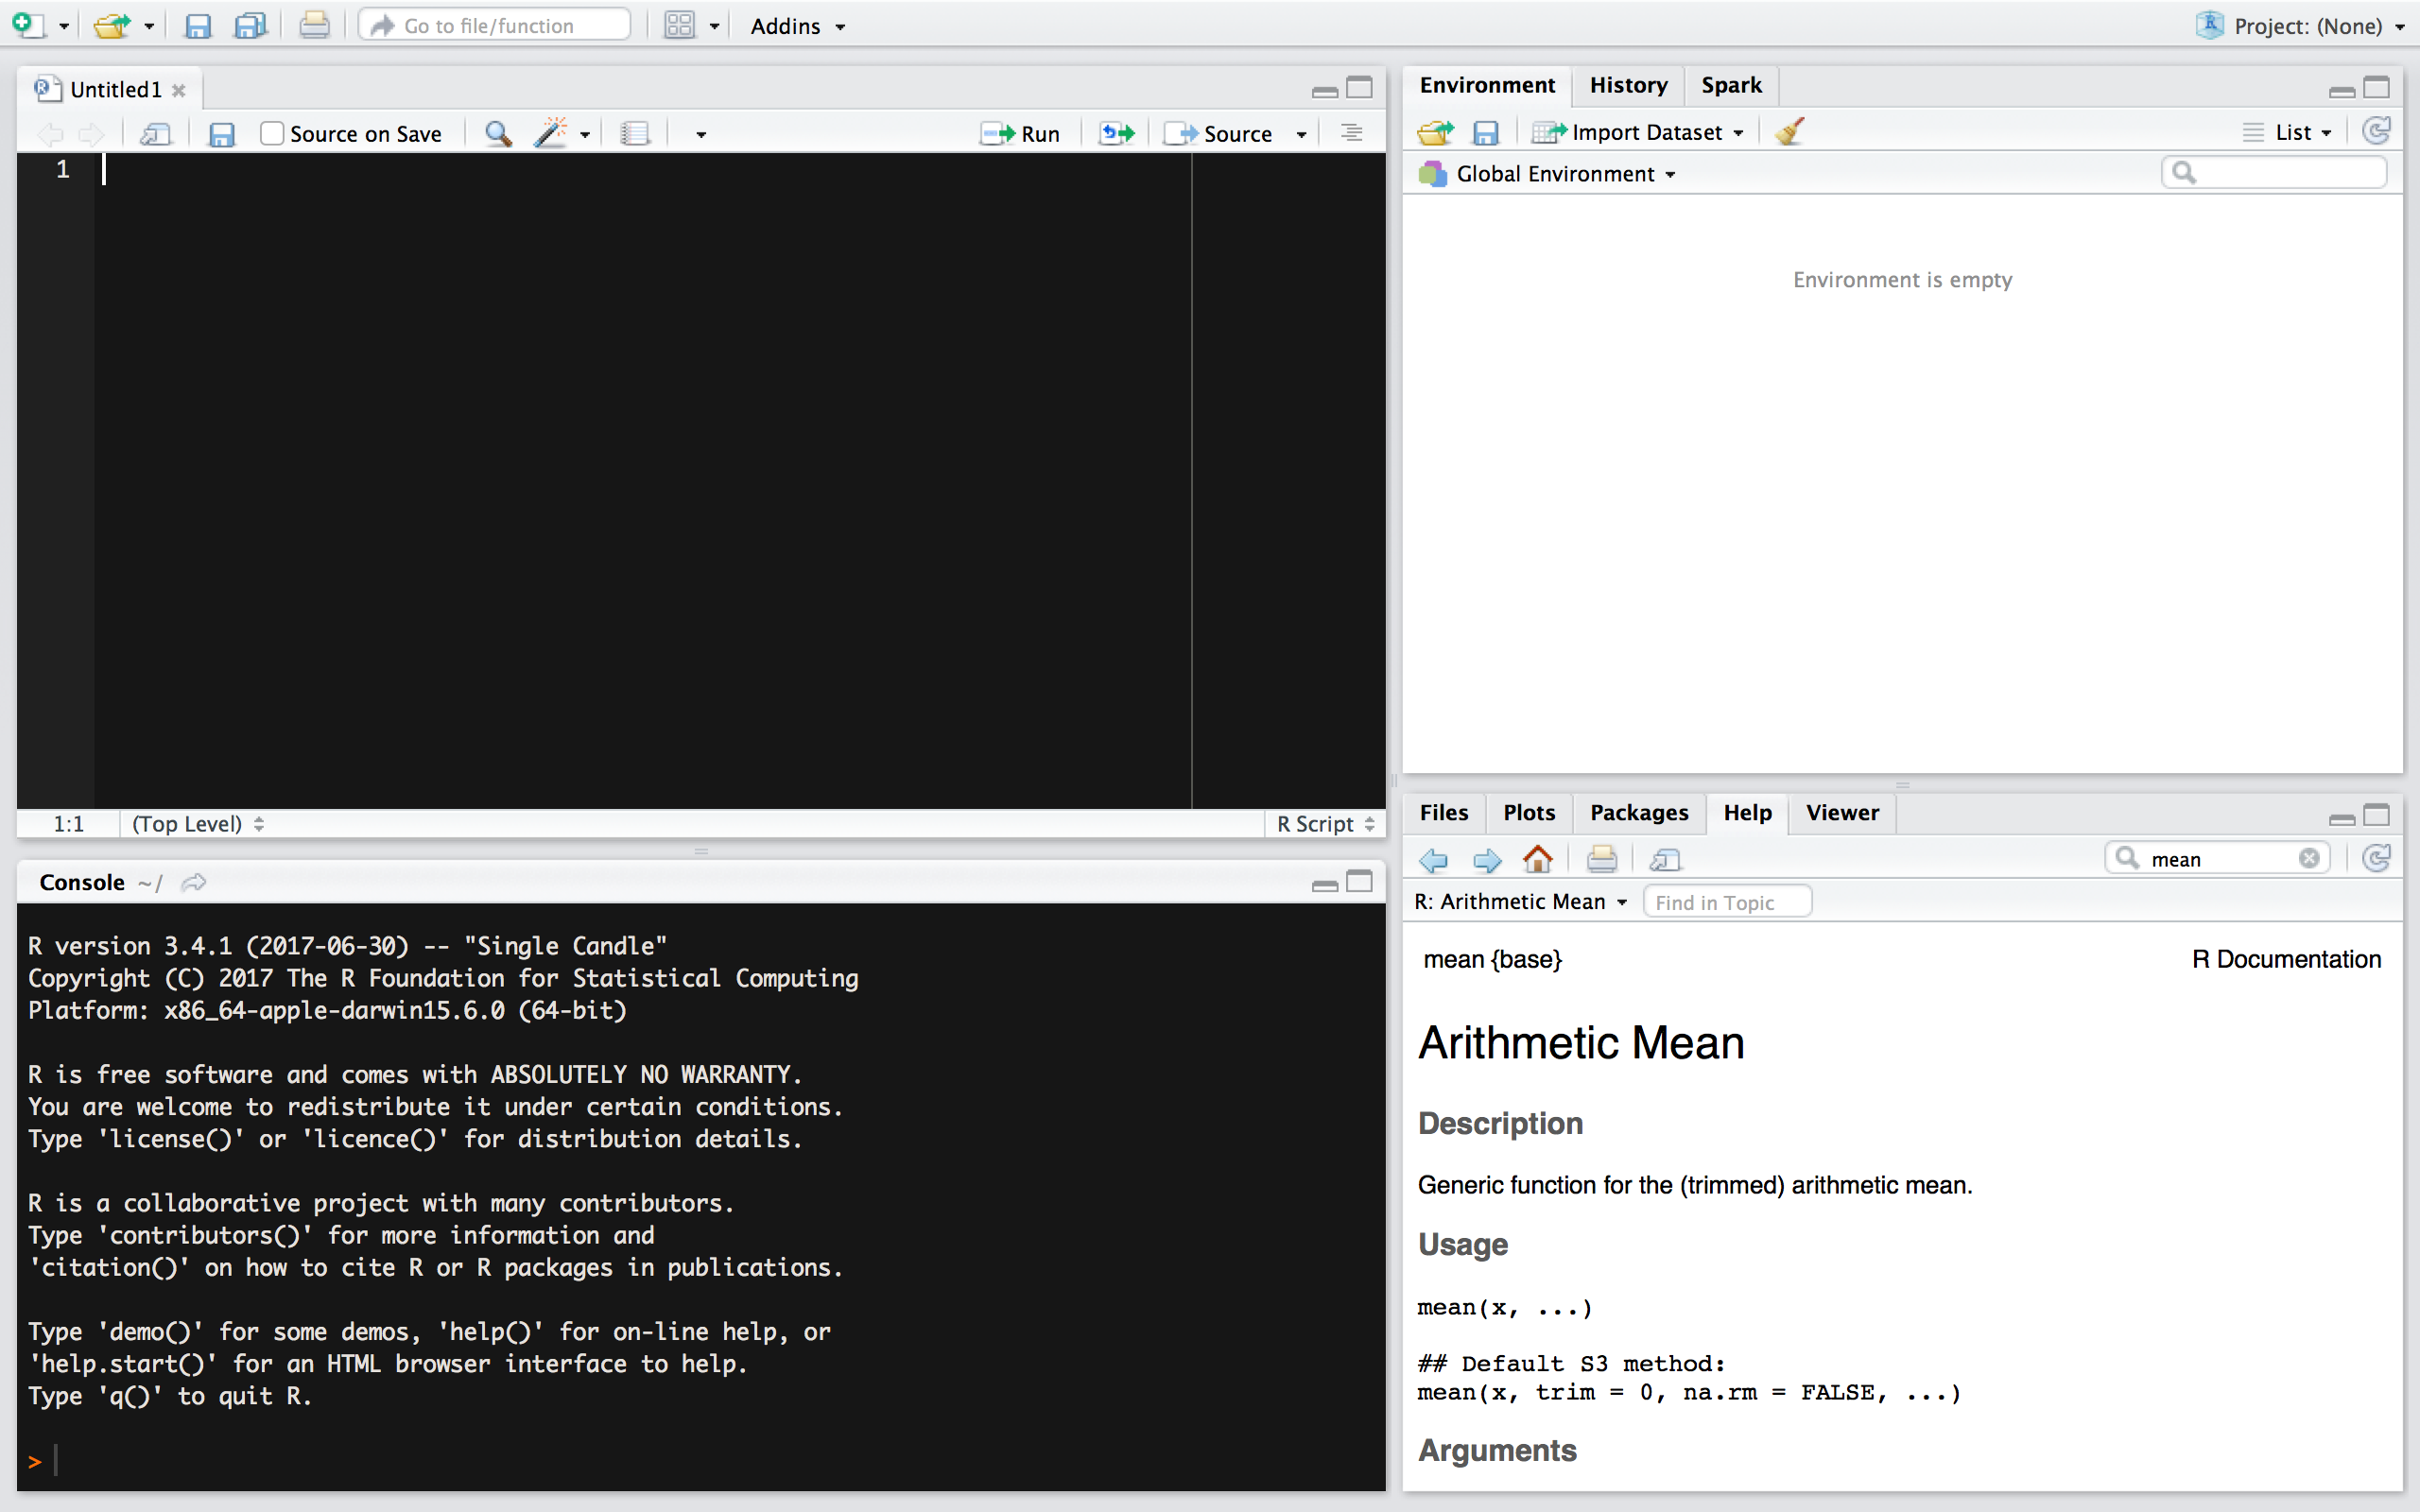
\includegraphics[width=35.56in]{assets/img/rstudio_screen_untitled} \caption{RStudio konsoolis on neli akent. Üleval vasakul on sinu poolt nimega varustatud koodi ja teksti editor kuhu kirjutad R skripti. Sinna kirjutad oma koodi ja kommentaarid sellele. All vasakul on konsool. Sinna sisestatakse käivitamisel sinu R kood ja sinna trükitakse väljund. Üleval paremal on Environment aken olulise sakiga <i class='fa fa-git' aria-hidden='true'></i>. Seal on näha R-i objektid, mis on sulle töökeskkonnas kättesaadavad ja millega sa saad töötada. <i class='fa fa-git' aria-hidden='true'></i> menüüs on võimalik muutusi vaadata ja 'commit'ida ja <i class='fa fa-github' aria-hidden='true'></i>-ga suhelda. All paremal on paneel mitme sakiga. Files tab töötab nagu failihaldur. Kui sa lood või avad R projekti, siis näidatakse seal vaikimisi sinu töökataloogi. Kui kasutad R projekti, siis ei ole vaja töökataloogi eraldi seadistada. Plots paneelile ilmuvad joonised, mille sa teed. Packages näitab sulle sinu arvutis olevaid R-i pakette ehk raamatukogusid. Help paneeli avanevad help failid (ka need, mida konsooli kaudu otsitakse).}\label{fig:rstudiowindow}
\end{figure}

Rohkem infot R projekti loomise kohta leiad RStudio infoleheküljelt:
\href{https://support.rstudio.com/hc/en-us/articles/200526207-Using-Projects}{Using
Projects}.

\section{\texorpdfstring{Git \emph{Merge}
konfliktid}{Git Merge konfliktid}}\label{git-merge-konfliktid}

Kollaboreerides üle GitHubi tekivad varem või hiljem konfliktid projekti
failide versioonide vahel nn. ``merge conflicts'', nende korrektselt
lahendama õppimine on väga oluline.

\begin{itemize}
\tightlist
\item
  Oma repo GitHubi veebilehel muuda/paranda README.md dokumenti ja
  ``Commit''-i seda lühisõnumiga mis sa muutsid/parandasid.
\item
  Seejärel, muuda oma arvutis olevat README.md faili RStudio-s viies
  sinna sisse mingi teistsuguse muudatuse. Tee ``Commit'' oma
  muudatustele.
\item
  Proovi ``push''-ida -- sa saad veateate!
\item
  Proovi ``pull''.
\item
  Lahenda ``merge'' konflikt ja seejärel ``commit'' + ``push''.
\end{itemize}

Githubi veateadete lugemine ja Google otsing aitavad sind.

\section{R projekti kataloogi soovitatav minimaalne
struktuur}\label{r-projekti-kataloogi-soovitatav-minimaalne-struktuur}

Iga R projekt peab olema täiesti iseseisev (\emph{selfcontained}) ja
sisaldama kogu infot, andmeid ja instruktsioone, et projektiga seotud
arvutused läbi viia ja raport genereerida. Kõik faili \emph{path}-id
peavad olema suhtelised.

R projekti kataloog peaks sisaldama projekti kirjeldavaid faile, mis
nimetatakse DESCRIPTION ja README.md. \textbf{DESCRIPTION} on tavaline
tekstifail ja sisaldab projekti metainfot ja infot projekti sõltuvuste
kohta, nagu väliste andmesettide asukoht, vajalik tarkvara jne.
\textbf{README.md} on markdown formaadis projekti info, sisaldab
juhendeid kasutajatele. Igale GitHubi repole on soovitav koostada
README.md, esialgu kasvõi projekti pealkiri ja üks kirjeldav lause.
README.md ja DESCRIPTION asuvad projekti juurkataloogis.

\begin{quote}
Projekti juurkataloogi jäävad ka kõik .Rmd laiendiga teksti ja analüüsi
tulemusi sisaldavad failid, millest genereeritakse lõplik
raport/dokument.
\end{quote}

Suuremad projektid, nagu näiteks teadusartikkel või raamat, võivad
sisaldada mitmeid Rmd faile ja võib tekkida kange kisatus need mõnda
alamkataloogi tõsta. Aga \texttt{knitr::knit()}, mis Rmarkdowni
markdowniks konverteerib, arvestab, et Rmd fail asub juurkataloogis ja
arvestab juurkataloogi suhtes ka failis olevaid \emph{path}-e teistele
failidele (näiteks ``data/my\_data.csv'').

\textbf{data/} kataloog sisaldab faile toorandmetega. Need failid peavad
olema R-i poolt loetavad ja soovitavalt tekstipõhised, laienditega TXT,
CSV, TSV jne. Neid faile ei muudeta, ainult loetakse. Kogu algandmete
töötlus toimub programmaatiliselt. Suured failid muudavad
versioonikontrolli aeglaseks, samuti on suheliselt mõttetu
versioonikontroll binaarsete failide korral (MS näiteks), sest diffid
pole lihtsalt inimkeeles. Github ütleb suurte failide kohta nii:
\emph{``GitHub will warn you when pushing files larger than 50 MB. You
will not be allowed to push files larger than 100 MB.''}

\textbf{src/} kataloog sisaldab analüüsi skripte, sealhulgas ka
andmetöötluse skripte.

\textbf{lib/} kataloogis on kasutaja poolt tehtud funktsioonide
definitsioone sisaldavad R skriptid.

\begin{verbatim}
project/
|- DESCRIPTION       # project metadata and dependencies
|- README.md         # description of contents and guide to users
|- my_analysis.Rmd   # markdown file containing analysis
|                    # writeup together with R code chunks
|
|- data/             # raw data, not changed once created 
|  +-my_data.csv     # data files in open formats, 
|                    # such as TXT, CSV, TSV etc.
|
|- src/              # any programmatic code
|  +-my_scripts.R    # R code used to analyse and 
|                    # visualise data
|
|- lib/              # user generated functions
|  +-my_functions.R  # R code defining functions
\end{verbatim}

On ka teisi konventsioone, näiteks R pakkide puhul paigutatakse kõik R
skriptid taaskasutatavate funktsioonidega kataloogi \textbf{R/}. Kui
selles kataloogis olevad skriptid on annoteeritud kasutades Roxygen-i
\citep{roxygen2}, siis genereeritakse automaatselt funktsioonide
dokumentatsioon kataloogi \textbf{man/}. Rohkem projekti pakkimise kohta
loe värskest preprindist ``Packaging data analytical work reproducibly
using R'' \citep{marwick2017}.

\chapter{Pakettide installeerimine}\label{pakettide-installeerimine}

R paketid sisaldavad ühte või enamat mingit kindlat operatsiooni läbi
viivat funktsiooni. Selleks, et installeerida pakett, sisesta järgnev
käsurida R konsooli:

\begin{Shaded}
\begin{Highlighting}[]
\NormalTok{## eg use "ggplot2" as packagename}
\KeywordTok{install.packages}\NormalTok{(}\StringTok{"packagename"}\NormalTok{)}
\end{Highlighting}
\end{Shaded}

RStudio võimaldab ka \emph{point-and-click} stiilis pakettide
installeerimist:

\begin{figure}
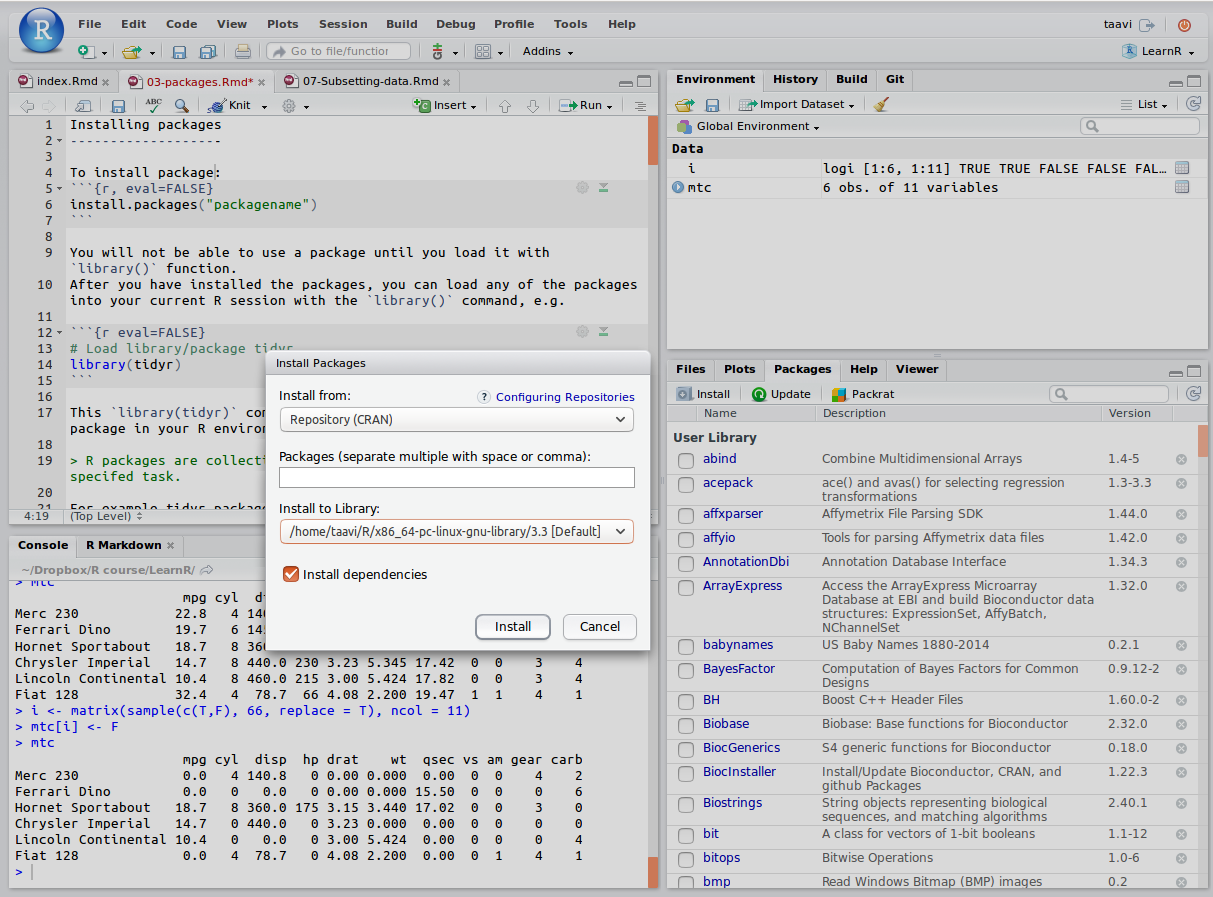
\includegraphics[width=16.85in]{assets/img/RStudio_package.install} \caption{RStudio 'Install Packages' dialoogiaken.}\label{fig:unnamed-chunk-2}
\end{figure}

\begin{quote}
Sa ei saa installeeritud pakette enne kasutada, kui laadid nad
töökeskkonda kasutades \texttt{library()} funktsiooni.
\end{quote}

Peale installeerimist lae pakett oma R sessiooni kasutades
\texttt{library()} käsku, näiteks:

\begin{Shaded}
\begin{Highlighting}[]
\NormalTok{## Load library/package tidyr}
\KeywordTok{library}\NormalTok{(tidyr)}
\end{Highlighting}
\end{Shaded}

\texttt{library(tidyr)} käsk teeb R sessioonis kasutatavaks kõik
``tidyr'' paketi funktsioonid.

Näiteks ``tidyr'' pakett sisaldab 41 funktsiooni:

\begin{Shaded}
\begin{Highlighting}[]
\KeywordTok{library}\NormalTok{(tidyr)}
\KeywordTok{ls}\NormalTok{(}\StringTok{"package:tidyr"}\NormalTok{)}
\end{Highlighting}
\end{Shaded}

\begin{verbatim}
##  [1] "%>%"             "complete"        "complete_"      
##  [4] "crossing"        "crossing_"       "drop_na"        
##  [7] "drop_na_"        "expand"          "expand_"        
## [10] "extract"         "extract_"        "extract_numeric"
## [13] "fill"            "fill_"           "full_seq"       
## [16] "gather"          "gather_"         "nest"           
## [19] "nest_"           "nesting"         "nesting_"       
## [22] "population"      "replace_na"      "separate"       
## [25] "separate_"       "separate_rows"   "separate_rows_" 
## [28] "smiths"          "spread"          "spread_"        
## [31] "table1"          "table2"          "table3"         
## [34] "table4a"         "table4b"         "table5"         
## [37] "unite"           "unite_"          "unnest"         
## [40] "unnest_"         "who"
\end{verbatim}

\section{R repositooriumid}\label{r-repositooriumid}

R pakid on saadaval kolmest põhilisest repositooriumist:

\begin{enumerate}
\def\labelenumi{\arabic{enumi}.}
\tightlist
\item
  \textbf{CRAN} \url{https://cran.r-project.org}
\end{enumerate}

\begin{Shaded}
\begin{Highlighting}[]
\KeywordTok{install.packages}\NormalTok{(}\StringTok{"ggplot2"}\NormalTok{)}
\end{Highlighting}
\end{Shaded}

\begin{enumerate}
\def\labelenumi{\arabic{enumi}.}
\setcounter{enumi}{1}
\tightlist
\item
  \textbf{Bioconductor} \url{https://www.bioconductor.org}
\end{enumerate}

\begin{Shaded}
\begin{Highlighting}[]
\CommentTok{# First run biocLite script fron bioconductor.org}
\KeywordTok{source}\NormalTok{(}\StringTok{"https://bioconductor.org/biocLite.R"}\NormalTok{)  }
\CommentTok{# use 'http' in url if 'https' is unavailable. }
\KeywordTok{biocLite}\NormalTok{(}\StringTok{"GenomicRanges"}\NormalTok{, }\DataTypeTok{suppressUpdates =} \OtherTok{TRUE}\NormalTok{)}
\end{Highlighting}
\end{Shaded}

\begin{enumerate}
\def\labelenumi{\arabic{enumi}.}
\setcounter{enumi}{2}
\tightlist
\item
  \textbf{GitHub} \url{https://github.com}
\end{enumerate}

\begin{Shaded}
\begin{Highlighting}[]
\NormalTok{## Näiteks järgnev käsk installeerib xaringan }
\NormalTok{## presentation ninja paketi}
\NormalTok{devtools}\OperatorTok{::}\KeywordTok{install_github}\NormalTok{(}\StringTok{"yihui/xaringan"}\NormalTok{)}
\end{Highlighting}
\end{Shaded}

\begin{quote}
NB! antud praktilise kursuse raames tutvume ja kasutame `tidyverse'
metapaketi funktsioone, laadides need iga sessiooni alguses:
\end{quote}

\begin{Shaded}
\begin{Highlighting}[]
\NormalTok{## install.packages("tidyverse")}
\KeywordTok{library}\NormalTok{(tidyverse)}
\end{Highlighting}
\end{Shaded}

\chapter{R on kalkulaator}\label{r-on-kalkulaator}

Selleks, et R aru saaks, et tegu on temale mõeldud käsu, aga mitte
tavatekstiga, Rmarkdown failis, tuleb see R koodirida spetsiaalsesse
\textbf{ümbrisesse või koodialasse} (i.k. \emph{chunk}) pakendada. Uue
koodiümbrise saad sisestada koodieditori servast ``Insert''
\textgreater{} ``R'' abil. Sisetatud R kood evalueeritakse siis, kui
vajutad tekinud hallis koodialas rohelisele nupule või alternatiivselt,
kui soovid jooksutada ainult osa koodi või üht koodirida, siis pane
kursor soovitud reale või võta osa koodi blokki ja vajuta klaviatuuril
cmd + enter.

Liidame \texttt{2\ +\ 2}.

\begin{Shaded}
\begin{Highlighting}[]
\DecValTok{2} \OperatorTok{+}\StringTok{ }\DecValTok{2}
\end{Highlighting}
\end{Shaded}

\begin{verbatim}
## [1] 4
\end{verbatim}

Nüüd trükiti see vastus konsooli kujul \texttt{{[}1{]}\ 4}. See
tähendab, et \texttt{2\ +\ 2\ =\ 4}.

Kontrollime seda:

\begin{Shaded}
\begin{Highlighting}[]
\NormalTok{answer <-}\StringTok{ }\DecValTok{2} \OperatorTok{+}\StringTok{ }\DecValTok{2} \OperatorTok{==}\StringTok{ }\DecValTok{4}
\NormalTok{## Trükime vastuse välja}
\NormalTok{answer}
\end{Highlighting}
\end{Shaded}

\begin{verbatim}
## [1] TRUE
\end{verbatim}

Vastus on TRUE, (logical).

Pane tähele, et aritmeetiline võrdusmärk on \texttt{==} (sest = tähendab
hoopis väärtuse määramist objektile/argumendile).

Veel mõned näidisarvutused:

\begin{Shaded}
\begin{Highlighting}[]
\CommentTok{# 3 astmes 2}
\DecValTok{3} \OperatorTok{**}\StringTok{ }\DecValTok{2}
\CommentTok{# Ruutjuur 3st}
\KeywordTok{sqrt}\NormalTok{(}\DecValTok{3}\NormalTok{)}
\CommentTok{# Naturaallogaritm sajast}
\KeywordTok{log}\NormalTok{(}\DecValTok{100}\NormalTok{)}
\end{Highlighting}
\end{Shaded}

Arvule \(\pi\) on määratud oma objekt \texttt{pi}. Seega on soovitav
enda poolt loodavatele objektidele mitte panna nimeks ``pi''.

\begin{Shaded}
\begin{Highlighting}[]
\CommentTok{# Ümarda pi neljale komakohale}
\KeywordTok{round}\NormalTok{(pi, }\DecValTok{4}\NormalTok{)}
\end{Highlighting}
\end{Shaded}

\begin{verbatim}
## [1] 3.1416
\end{verbatim}

Ümardamine on oluline tulemuste väljaprintimisel.

\section{R objektid}\label{r-objektid}

R-i töökeskkonnas ``workspace'' asuvad \textbf{objektid}, millega me
töötame. Tüüpilised objektid on:

\begin{itemize}
\tightlist
\item
  Andmekogud (vektorid, tabelid, maatriksid, listid jm).
\item
  Statistiliste analüüside väljundid.
\item
  Funktsioonid, mille oleme ise sisse lugenud.
\end{itemize}

Käsk \texttt{ls()} annab objektide nimed teie workspace-s:

\begin{Shaded}
\begin{Highlighting}[]
\KeywordTok{ls}\NormalTok{()}
\end{Highlighting}
\end{Shaded}

\begin{verbatim}
## [1] "answer"
\end{verbatim}

\texttt{rm(a)} removes object a from the workspace

Selleks, et salvestada töökeskkond faili kasuta ``Save'' nuppu
``Environment'' akna servast või menüüst ``Session'' -\textgreater{}
``Save Workspace As''.

\subsection{Objekt ja nimi}\label{objekt-ja-nimi}

kui teil sünnib laps, annate talle nime.

R-s on vastupidi: nimele antakse objekt

\begin{Shaded}
\begin{Highlighting}[]
\NormalTok{babe <-}\StringTok{ "beebi"}
\NormalTok{babe}
\end{Highlighting}
\end{Shaded}

\begin{verbatim}
## [1] "beebi"
\end{verbatim}

Siin on kõigepealt nimi (babe), siis assingmenti sümbol \textless{}- ja
lõpuks objekt, mis on nimele antud (string ``beebi'').

NB! stringid on jutumärkides, nimed mitte

nimi üksi evalueeritakse kui ``print object'', mis antud juhul on string
``beebi''

Nüüd muudame objekti nime taga

\begin{Shaded}
\begin{Highlighting}[]
\NormalTok{babe <-}\StringTok{ }\KeywordTok{c}\NormalTok{(}\StringTok{"saatan"}\NormalTok{, }\StringTok{"inglike"}\NormalTok{)}
\NormalTok{babe}
\end{Highlighting}
\end{Shaded}

\begin{verbatim}
## [1] "saatan"  "inglike"
\end{verbatim}

Tulemuseks on sama nimi, mis tähistab nüüd midagi muud (vektorit, mis
koosneb 2st stringist). Objekt ``beebi'' kaotas oma nime ja on nüüd
workspacest kadunud.

\begin{Shaded}
\begin{Highlighting}[]
\KeywordTok{class}\NormalTok{(babe)}
\end{Highlighting}
\end{Shaded}

\begin{verbatim}
## [1] "character"
\end{verbatim}

class() annab meile objekti tüübi. Antud juhul \emph{character vector}.

\begin{quote}
Ainult need objektid, mis on assigneeritud nimele, lähevad workspace ja
on sellistena kasutatvad edasises analüüsis.
\end{quote}

\begin{Shaded}
\begin{Highlighting}[]
\NormalTok{apples <-}\StringTok{ }\DecValTok{2}
\NormalTok{bananas <-}\StringTok{ }\DecValTok{3}
\NormalTok{apples }\OperatorTok{+}\StringTok{ }\NormalTok{bananas}
\end{Highlighting}
\end{Shaded}

\begin{verbatim}
## [1] 5
\end{verbatim}

objekt 5 ei ole nimetatud, seega ei ilmu see ka workspace

\begin{Shaded}
\begin{Highlighting}[]
\NormalTok{a <-}\StringTok{ }\DecValTok{2}
\NormalTok{b <-}\StringTok{ }\DecValTok{3}
\NormalTok{a <-}\StringTok{ }\NormalTok{a}\OperatorTok{+}\NormalTok{b}
\KeywordTok{str}\NormalTok{(a) }\CommentTok{#objekti nimega a struktuur}
\end{Highlighting}
\end{Shaded}

\begin{verbatim}
##  num 5
\end{verbatim}

Nüüd on nimega a seostatud uus objekt, mis koosneb numbrist 5 (olles ühe
elemendiga vektor). Ja nimega a eelnevalt seostatud objekt, mis koosnes
numbrist 2, on workspacest lahkunud.

\subsubsection{Nimede vorm}\label{nimede-vorm}

\begin{itemize}
\item
  Nimed algavad tähemärgiga, mitte numbriga ega
  \$\euro{}\%\&/?\textasciitilde{}ˇöõüä
\item
  Nimed ei sisalda tühikuid
\item
  Tühiku asemel kasuta alakriipsu: näiteks eriti\_pikk\_nimi
\item
  SUURED ja väiksed tähed on nimes erinevad
\item
  Nimed peaksid kirjeldama objekti, mis on sellele nimele assigneeritud
  ja nad võivad olla pikad sest TAB klahv annab meile auto-complete.
\item
  alt + - on otsetee \textless{}- jaoks
\end{itemize}

\subsubsection{Sama koodi saab kirjutada neljal
viisil}\label{sama-koodi-saab-kirjutada-neljal-viisil}

Hargnevate teede aed: kui me muudame olemasolevat objekti on meil alati
kaks valikut. Me kas jätame muudetud objektile vana objekti nime või me
anname talle uue nime. Esimesel juhul läheb vana muutmata objekt
workspacest kaduma aga nimesid ei tule juurde ja säilib teatud workflow
sujuvus. Teisel juhul jäävad analüüsi vaheobjektid meile alles ja nende
juurde saab alati tagasi tulla. Samas tekkib meile palju sarnaste
nimedega objekte.

Esimnene võimalus

\begin{Shaded}
\begin{Highlighting}[]
\NormalTok{a <-}\StringTok{ }\KeywordTok{c}\NormalTok{(}\DecValTok{2}\NormalTok{, }\DecValTok{3}\NormalTok{)}
\NormalTok{a <-}\StringTok{ }\KeywordTok{sum}\NormalTok{(a)}
\NormalTok{a <-}\StringTok{ }\KeywordTok{sqrt}\NormalTok{(a)}
\NormalTok{a <-}\StringTok{ }\KeywordTok{round}\NormalTok{(a, }\DecValTok{2}\NormalTok{)}
\NormalTok{a}
\end{Highlighting}
\end{Shaded}

\begin{verbatim}
## [1] 2.24
\end{verbatim}

Teine võimalus

\begin{Shaded}
\begin{Highlighting}[]
\NormalTok{a <-}\StringTok{ }\KeywordTok{c}\NormalTok{(}\DecValTok{2}\NormalTok{, }\DecValTok{3}\NormalTok{)}
\NormalTok{a1 <-}\StringTok{ }\KeywordTok{sum}\NormalTok{(a)}
\NormalTok{a2 <-}\StringTok{ }\KeywordTok{sqrt}\NormalTok{(a1)}
\NormalTok{a3 <-}\StringTok{ }\KeywordTok{round}\NormalTok{(a2, }\DecValTok{2}\NormalTok{)}
\NormalTok{a3}
\end{Highlighting}
\end{Shaded}

\begin{verbatim}
## [1] 2.24
\end{verbatim}

Kolmas võimalus on lühem variant esimesest. Me nimelt ühendame etapid
toru \texttt{\%\textgreater{}\%} kaudu. Siin me võtame objekti a (nö.
andmed), suuname selle funktsiooni \texttt{sum()}, võtame selle
funktsiooni väljundi ja suuname selle omakorda funktsiooni
\texttt{sqrt()}. Seejärel võtame selle funktsiooni outputi ja määrame
selle nimele ``result'' (aga võime selle ka mõne teise nimega siduda).
Kui mõni funktsioon võtab ainult ühe parameetri, mille me talle toru
kaudu sisse sõõdame, siis pole selle funktsiooni taga isegi sulge vaja.
NB! R hea stiili juhised soovitavad siiski ka sellisel juhul kasutada
funktsiooni koos sulgudega! See on hea lühike ja inimloetav viis koodi
kirjutada, mis on masina jaoks identne esimese koodiga.

\begin{Shaded}
\begin{Highlighting}[]
\NormalTok{## we need piping operator '%>%' from magrittr}
\KeywordTok{library}\NormalTok{(magrittr)}
\NormalTok{a <-}\StringTok{ }\KeywordTok{c}\NormalTok{(}\DecValTok{2}\NormalTok{, }\DecValTok{3}\NormalTok{)}
\NormalTok{result <-}\StringTok{ }\NormalTok{a }\OperatorTok\StringTok{ }\KeywordTok{sum}\NormalTok{() }\OperatorTok\StringTok{ }\KeywordTok{sqrt}\NormalTok{() }\OperatorTok\StringTok{ }\KeywordTok{round}\NormalTok{(}\DecValTok{2}\NormalTok{)}
\NormalTok{result}
\end{Highlighting}
\end{Shaded}

\begin{verbatim}
## [1] 2.24
\end{verbatim}

Neljas võimalus: Kõrgharitud programmeerija kirjutaks selle koodi aga
nii:

\begin{Shaded}
\begin{Highlighting}[]
\NormalTok{a <-}\StringTok{ }\KeywordTok{c}\NormalTok{(}\DecValTok{2}\NormalTok{, }\DecValTok{3}\NormalTok{)}
\NormalTok{a <-}\StringTok{ }\KeywordTok{round}\NormalTok{(}\KeywordTok{sqrt}\NormalTok{(}\KeywordTok{sum}\NormalTok{(a)), }\DecValTok{2}\NormalTok{)}
\NormalTok{a}
\end{Highlighting}
\end{Shaded}

\begin{verbatim}
## [1] 2.24
\end{verbatim}

Sellist koodi loetakse keskelt väljappoole ja kirjutattakse alates
viimasest operatsioonist, mida soovitakse, et kood teeks. Masina jaoks
pole vahet. Inimese jaoks on küll: 4. variant nõuab hästi pestud ajusid.

Koodi lühidus 4 --\textgreater{} 3 --\textgreater{} 1 --\textgreater{} 2
(pikem)

lollikindlus 1 --\textgreater{} 2 --\textgreater{} 3 --\textgreater{} 4
(vähem lollikindel)

Mida vähem on kohti, kus saab koodi töötamist kontrollida, seda halvem
teile. Sellepärast ärge kunagi pange üksteise otsa rohkem kui 4
torujuppi. See on teie otsustada, millist koodivormi te millal kasutate,
aga te peaksite oskama lugeda neid kõiki.

\section{Objektide tüübid}\label{objektide-tuubid}

\subsection{Vektor - andmerida}\label{vektor---andmerida}

Vektor on rida kindlas järjekorras arve, tähemärke või TRUE/FALSE
loogilisi väärtusi. Iga vektor sisaldab ainult ühte tüüpi andmeid.
Vektor on elementaarüksus, millega me teeme tehteid. Andmetabelis
ripuvad kõrvuti ühepikad vektorid (üks vektor = üks tulp) ja R-le
meeldib arvutada vektori kaupa vasakult paremale (mis tabelis on ülevalt
alla sest vektori algus on üleval tabeli headeri juures). Vektori
loomiseks kasuta funktsiooni c() --- combine

\begin{Shaded}
\begin{Highlighting}[]
\NormalTok{minu_vektor <-}\StringTok{ }\KeywordTok{c}\NormalTok{(}\DecValTok{1}\NormalTok{, }\DecValTok{3}\NormalTok{, }\DecValTok{4}\NormalTok{)}
\KeywordTok{str}\NormalTok{(minu_vektor)}
\end{Highlighting}
\end{Shaded}

\begin{verbatim}
##  num [1:3] 1 3 4
\end{verbatim}

\begin{Shaded}
\begin{Highlighting}[]
\NormalTok{minu_vektor <-}\StringTok{ }\KeywordTok{c}\NormalTok{(}\DecValTok{1}\NormalTok{, }\OtherTok{NA}\NormalTok{, }\DecValTok{4}\NormalTok{)}
\NormalTok{minu_vektor}
\end{Highlighting}
\end{Shaded}

\begin{verbatim}
## [1]  1 NA  4
\end{verbatim}

\begin{Shaded}
\begin{Highlighting}[]
\KeywordTok{class}\NormalTok{(minu_vektor)}
\end{Highlighting}
\end{Shaded}

\begin{verbatim}
## [1] "numeric"
\end{verbatim}

\begin{Shaded}
\begin{Highlighting}[]
\NormalTok{minu_vektor <-}\StringTok{ }\KeywordTok{c}\NormalTok{(}\DecValTok{1}\NormalTok{, }\StringTok{"A1"}\NormalTok{, }\StringTok{"4$"}\NormalTok{, }\StringTok{"joe"}\NormalTok{)}
\NormalTok{minu_vektor}
\end{Highlighting}
\end{Shaded}

\begin{verbatim}
## [1] "1"   "A1"  "4$"  "joe"
\end{verbatim}

\begin{Shaded}
\begin{Highlighting}[]
\KeywordTok{class}\NormalTok{(minu_vektor)}
\end{Highlighting}
\end{Shaded}

\begin{verbatim}
## [1] "character"
\end{verbatim}

Piisab ühest tõrvatilgast meepotis, et teie vektor ei sisaldaks enam
numbreid.

Järgneva trikiga saab mitte-numbrilisest vektorist numbrilise vektori.

\begin{Shaded}
\begin{Highlighting}[]
\KeywordTok{library}\NormalTok{(readr)}
\NormalTok{minu_vektor <-}\StringTok{ }\KeywordTok{as.vector}\NormalTok{(}\KeywordTok{parse_number}\NormalTok{(minu_vektor))}
\end{Highlighting}
\end{Shaded}

\begin{verbatim}
## Warning: 1 parsing failure.
## row # A tibble: 1 x 4 col     row   col expected actual expected   <int> <int>    <chr>  <chr> actual 1     4    NA a number    joe
\end{verbatim}

\begin{Shaded}
\begin{Highlighting}[]
\NormalTok{minu_vektor}
\end{Highlighting}
\end{Shaded}

\begin{verbatim}
## [1]  1  1  4 NA
\end{verbatim}

\begin{Shaded}
\begin{Highlighting}[]
\KeywordTok{str}\NormalTok{(minu_vektor)}
\end{Highlighting}
\end{Shaded}

\begin{verbatim}
##  num [1:4] 1 1 4 NA
\end{verbatim}

\begin{Shaded}
\begin{Highlighting}[]
\KeywordTok{sort}\NormalTok{(x, }\DataTypeTok{decreasing =} \OtherTok{FALSE}\NormalTok{, ...) }\CommentTok{#sorts vector in ascending order}
\KeywordTok{unique}\NormalTok{(x) }\CommentTok{#returns a vector or data frame, but with duplicate elements/rows removed.}
\end{Highlighting}
\end{Shaded}

\subsection{\texorpdfstring{Uus vektor: \texttt{seq()} ja
\texttt{rep()}}{Uus vektor: seq() ja rep()}}\label{uus-vektor-seq-ja-rep}

\begin{Shaded}
\begin{Highlighting}[]
\KeywordTok{seq}\NormalTok{(}\DecValTok{2}\NormalTok{, }\DecValTok{3}\NormalTok{, }\DataTypeTok{by =} \FloatTok{0.5}\NormalTok{)}
\end{Highlighting}
\end{Shaded}

\begin{verbatim}
## [1] 2.0 2.5 3.0
\end{verbatim}

\begin{Shaded}
\begin{Highlighting}[]
\KeywordTok{seq}\NormalTok{(}\DecValTok{2}\NormalTok{, }\DecValTok{3}\NormalTok{, }\DataTypeTok{length.out =} \DecValTok{5}\NormalTok{)}
\end{Highlighting}
\end{Shaded}

\begin{verbatim}
## [1] 2.00 2.25 2.50 2.75 3.00
\end{verbatim}

\begin{Shaded}
\begin{Highlighting}[]
\KeywordTok{rep}\NormalTok{(}\DecValTok{1}\OperatorTok{:}\DecValTok{2}\NormalTok{, }\DataTypeTok{times =} \DecValTok{3}\NormalTok{)}
\end{Highlighting}
\end{Shaded}

\begin{verbatim}
## [1] 1 2 1 2 1 2
\end{verbatim}

\begin{Shaded}
\begin{Highlighting}[]
\KeywordTok{rep}\NormalTok{(}\DecValTok{1}\OperatorTok{:}\DecValTok{2}\NormalTok{, }\DataTypeTok{each =} \DecValTok{3}\NormalTok{)}
\end{Highlighting}
\end{Shaded}

\begin{verbatim}
## [1] 1 1 1 2 2 2
\end{verbatim}

\begin{Shaded}
\begin{Highlighting}[]
\KeywordTok{rep}\NormalTok{(}\KeywordTok{c}\NormalTok{(}\StringTok{"a"}\NormalTok{, }\StringTok{"b"}\NormalTok{), }\DataTypeTok{each =} \DecValTok{3}\NormalTok{, }\DataTypeTok{times =} \DecValTok{2}\NormalTok{)}
\end{Highlighting}
\end{Shaded}

\begin{verbatim}
##  [1] "a" "a" "a" "b" "b" "b" "a" "a" "a" "b" "b" "b"
\end{verbatim}

\subsection{tehted arvuliste
vektoritega}\label{tehted-arvuliste-vektoritega}

Vektoreid saab liita, lahutada, korrutada ja jagada.

\begin{Shaded}
\begin{Highlighting}[]
\NormalTok{a <-}\StringTok{ }\KeywordTok{c}\NormalTok{(}\DecValTok{1}\NormalTok{,}\DecValTok{2}\NormalTok{,}\DecValTok{3}\NormalTok{)}
\NormalTok{b <-}\StringTok{ }\DecValTok{4} \CommentTok{#ühe elemendiga vektor ei vaja c() enda ümber}
\NormalTok{a }\OperatorTok{+}\StringTok{ }\NormalTok{b}
\end{Highlighting}
\end{Shaded}

\begin{verbatim}
## [1] 5 6 7
\end{verbatim}

Kõik vektor a liikmed liideti arvuga 3 (kuna vektor b koosnes ühest
liikmest, läks see kordusesse)

\begin{Shaded}
\begin{Highlighting}[]
\NormalTok{a <-}\StringTok{ }\KeywordTok{c}\NormalTok{(}\DecValTok{1}\NormalTok{, }\DecValTok{2}\NormalTok{, }\DecValTok{3}\NormalTok{)}
\NormalTok{b <-}\StringTok{ }\KeywordTok{c}\NormalTok{(}\DecValTok{4}\NormalTok{, }\DecValTok{5}\NormalTok{) }
\NormalTok{a }\OperatorTok{+}\StringTok{ }\NormalTok{b}
\end{Highlighting}
\end{Shaded}

\begin{verbatim}
## Warning in a + b: longer object length is not a multiple of shorter object
## length
\end{verbatim}

\begin{verbatim}
## [1] 5 7 7
\end{verbatim}

Aga see töötab veateatega, sest vektorite pikkused ei ole üksteise
kordajad 1 + 4; 2 + 5, 3 + 4

\begin{Shaded}
\begin{Highlighting}[]
\NormalTok{a <-}\StringTok{ }\KeywordTok{c}\NormalTok{(}\DecValTok{1}\NormalTok{, }\DecValTok{2}\NormalTok{, }\DecValTok{3}\NormalTok{, }\DecValTok{4}\NormalTok{)}
\NormalTok{b <-}\StringTok{ }\KeywordTok{c}\NormalTok{(}\DecValTok{5}\NormalTok{, }\DecValTok{6}\NormalTok{) }
\NormalTok{a }\OperatorTok{+}\StringTok{ }\NormalTok{b}
\end{Highlighting}
\end{Shaded}

\begin{verbatim}
## [1]  6  8  8 10
\end{verbatim}

see töötab: 1 + 5; 2 + 6; 3 + 5; 4 + 6

\begin{Shaded}
\begin{Highlighting}[]
\NormalTok{a <-}\StringTok{ }\KeywordTok{c}\NormalTok{(}\DecValTok{1}\NormalTok{, }\DecValTok{2}\NormalTok{, }\DecValTok{3}\NormalTok{, }\DecValTok{4}\NormalTok{)}
\NormalTok{b <-}\StringTok{ }\KeywordTok{c}\NormalTok{(}\DecValTok{5}\NormalTok{, }\DecValTok{6}\NormalTok{, }\DecValTok{7}\NormalTok{, }\DecValTok{8}\NormalTok{) }
\NormalTok{a }\OperatorTok{+}\StringTok{ }\NormalTok{b}
\end{Highlighting}
\end{Shaded}

\begin{verbatim}
## [1]  6  8 10 12
\end{verbatim}

Samuti see (ühepikkused vektorid --- igat liiget kasutatakse üks kord)

\begin{Shaded}
\begin{Highlighting}[]
\NormalTok{a <-}\StringTok{ }\KeywordTok{c}\NormalTok{(}\OtherTok{TRUE}\NormalTok{, }\OtherTok{FALSE}\NormalTok{, }\OtherTok{TRUE}\NormalTok{)}
\KeywordTok{sum}\NormalTok{(a)}
\end{Highlighting}
\end{Shaded}

\begin{verbatim}
## [1] 2
\end{verbatim}

\begin{Shaded}
\begin{Highlighting}[]
\KeywordTok{mean}\NormalTok{(a)}
\end{Highlighting}
\end{Shaded}

\begin{verbatim}
## [1] 0.6666667
\end{verbatim}

Mis siin juhtus? R kodeerib sisemiselt TRUE kui 1 ja FALSE kui 0-i.
summa 1 + 0 + 1 = 2. Seda loogiliste väärtuste omadust õpime varsti
praktikas kasutama.

\subsection{List -- andmekott}\label{list-andmekott}

List on objektitüüp, kuhu saab koondada kõiki teisi objekte, kaasa
arvatud listid. See on lihtsalt viis objektid koos hoida ühes suuremas
meta-objektis. List on nagu jõuluvana kingikott, kus kommid, sokipaarid
ja muud kingid kõik segamini loksuvad.

Näiteks siin list, kus loksuvad 1 vektor nimega a, 1 tibble nimega b ja
1 list nimega c, mis omakorda sisaldab vektorit nimega d ja tibblet
nimega e. Seega on meil tegu rekursiivse listiga.

\begin{Shaded}
\begin{Highlighting}[]
\CommentTok{# numeric vector a}
\NormalTok{a <-}\StringTok{ }\KeywordTok{runif}\NormalTok{(}\DecValTok{5}\NormalTok{)}
\CommentTok{# data.frame}
\NormalTok{ab <-}\StringTok{ }\KeywordTok{data.frame}\NormalTok{(a, }\DataTypeTok{b =} \KeywordTok{rnorm}\NormalTok{(}\DecValTok{5}\NormalTok{))}
\CommentTok{# linear model}
\NormalTok{model <-}\StringTok{ }\KeywordTok{lm}\NormalTok{(mpg }\OperatorTok{~}\StringTok{ }\NormalTok{hp, }\DataTypeTok{data =}\NormalTok{ mtcars)}
\CommentTok{# your grandma on bongos}
\NormalTok{grandma <-}\StringTok{ "your grandma on bongos"}
\CommentTok{# let's creat list}
\NormalTok{happy_list <-}\StringTok{ }\KeywordTok{list}\NormalTok{(a, ab, model, grandma)}
\NormalTok{happy_list}
\end{Highlighting}
\end{Shaded}

\begin{verbatim}
## [[1]]
## [1] 0.17657487 0.28478609 0.07219848 0.67306296 0.98082175
## 
## [[2]]
##            a          b
## 1 0.17657487  0.2104119
## 2 0.28478609  1.5843747
## 3 0.07219848 -1.8728558
## 4 0.67306296 -0.2245067
## 5 0.98082175 -0.3536892
## 
## [[3]]
## 
## Call:
## lm(formula = mpg ~ hp, data = mtcars)
## 
## Coefficients:
## (Intercept)           hp  
##    30.09886     -0.06823  
## 
## 
## [[4]]
## [1] "your grandma on bongos"
\end{verbatim}

võtame listist välja elemndi ``ab'':

\begin{Shaded}
\begin{Highlighting}[]
\NormalTok{happy_list}\OperatorTok{$}\NormalTok{ab}
\end{Highlighting}
\end{Shaded}

\begin{verbatim}
## NULL
\end{verbatim}

\section{Tibble ja data frame -
andmeraamid}\label{tibble-ja-data-frame---andmeraamid}

\begin{Shaded}
\begin{Highlighting}[]
\KeywordTok{library}\NormalTok{(tidyverse)}
\end{Highlighting}
\end{Shaded}

Andmeraam on eriline list, mis koosneb ühepikkustest vektoritest.
Andmeraam on ühtlasi teatud liiki tabel, kus igas veerus on ainult ühte
tüüpi andmed. Need vektorid ripuvad andmeraamis kõrvuti nagu tuulehaugid
suitsuahjus, kusjuures vektori algus vastab tuulehaugi peale, mis on
konksu otsas (konks vastab andmeraamis tulba nimele ja ühtlasi vektori
nimele). Iga vektori nimi muutub sellises tabelis tulba nimeks. Igas
tulbas saab olla ainult ühte tüüpi andmeid.

R-s on 2 andmeraami tüüpi: tibble ja data frame, mis on väga sarnased.
Tibble on uuem, veidi kaunima väljatrükiga, pisut mugavam kasutada, ja
me kasutame põhiliselt seda, välja arvatud hiljem Bayesi arvutustes, kus
me tehnilistel põhjustel kasutame data frame. Tidyverse töötab tibblega
veidi paremini kui data frame-ga, aga see vahe ei ole suur.

siin on meil 3 vektorit: shop, apples ja oranges, millest me paneme
kokku tibble nimega fruits

\begin{Shaded}
\begin{Highlighting}[]
\NormalTok{shop <-}\StringTok{ }\KeywordTok{c}\NormalTok{(}\StringTok{"maxima"}\NormalTok{, }\StringTok{"tesco"}\NormalTok{, }\StringTok{"lidl"}\NormalTok{)}
\NormalTok{apples <-}\StringTok{ }\KeywordTok{c}\NormalTok{(}\DecValTok{1}\NormalTok{, }\DecValTok{4}\NormalTok{, }\DecValTok{43}\NormalTok{)}
\NormalTok{oranges <-}\StringTok{ }\KeywordTok{c}\NormalTok{(}\DecValTok{2}\NormalTok{, }\DecValTok{32}\NormalTok{, }\OtherTok{NA}\NormalTok{)}
\NormalTok{fruits <-}\StringTok{ }\KeywordTok{tibble}\NormalTok{(shop, apples, oranges)}
\NormalTok{fruits}
\end{Highlighting}
\end{Shaded}

\begin{verbatim}
## # A tibble: 3 x 3
##     shop apples oranges
##    <chr>  <dbl>   <dbl>
## 1 maxima      1       2
## 2  tesco      4      32
## 3   lidl     43      NA
\end{verbatim}

Siin ta on, ilusti meie workspace-s.

\textbf{Mõned asjad, mida tibblega (ja data framega) saab teha:}

\begin{Shaded}
\begin{Highlighting}[]
\KeywordTok{count}\NormalTok{(fruits, apples)}
\end{Highlighting}
\end{Shaded}

\begin{verbatim}
## # A tibble: 3 x 2
##   apples     n
##    <dbl> <int>
## 1      1     1
## 2      4     1
## 3     43     1
\end{verbatim}

\begin{Shaded}
\begin{Highlighting}[]
\KeywordTok{count}\NormalTok{(fruits, shop)}
\end{Highlighting}
\end{Shaded}

\begin{verbatim}
## # A tibble: 3 x 2
##     shop     n
##    <chr> <int>
## 1   lidl     1
## 2 maxima     1
## 3  tesco     1
\end{verbatim}

\begin{Shaded}
\begin{Highlighting}[]
\KeywordTok{summary}\NormalTok{(fruits)}
\end{Highlighting}
\end{Shaded}

\begin{verbatim}
##      shop               apples        oranges    
##  Length:3           Min.   : 1.0   Min.   : 2.0  
##  Class :character   1st Qu.: 2.5   1st Qu.: 9.5  
##  Mode  :character   Median : 4.0   Median :17.0  
##                     Mean   :16.0   Mean   :17.0  
##                     3rd Qu.:23.5   3rd Qu.:24.5  
##                     Max.   :43.0   Max.   :32.0  
##                                    NA's   :1
\end{verbatim}

\begin{Shaded}
\begin{Highlighting}[]
\KeywordTok{names}\NormalTok{(fruits)}
\end{Highlighting}
\end{Shaded}

\begin{verbatim}
## [1] "shop"    "apples"  "oranges"
\end{verbatim}

\begin{Shaded}
\begin{Highlighting}[]
\KeywordTok{colnames}\NormalTok{(fruits)}
\end{Highlighting}
\end{Shaded}

\begin{verbatim}
## [1] "shop"    "apples"  "oranges"
\end{verbatim}

\begin{Shaded}
\begin{Highlighting}[]
\KeywordTok{nrow}\NormalTok{(fruits)}
\end{Highlighting}
\end{Shaded}

\begin{verbatim}
## [1] 3
\end{verbatim}

\begin{Shaded}
\begin{Highlighting}[]
\KeywordTok{ncol}\NormalTok{(fruits)}
\end{Highlighting}
\end{Shaded}

\begin{verbatim}
## [1] 3
\end{verbatim}

\begin{Shaded}
\begin{Highlighting}[]
\KeywordTok{arrange}\NormalTok{(fruits, }\KeywordTok{desc}\NormalTok{(apples)) }\CommentTok{#sorteerib tabeli veeru "apples" väärtuste järgi langevalt (default on tõusev sorteerimine). Võib argumendina anda mitu veergu.}
\end{Highlighting}
\end{Shaded}

\begin{verbatim}
## # A tibble: 3 x 3
##     shop apples oranges
##    <chr>  <dbl>   <dbl>
## 1   lidl     43      NA
## 2  tesco      4      32
## 3 maxima      1       2
\end{verbatim}

\begin{Shaded}
\begin{Highlighting}[]
\KeywordTok{top_n}\NormalTok{(fruits, }\DecValTok{2}\NormalTok{, apples) }\CommentTok{#saab 2 rida, milles on kõige rohkem õunu}
\end{Highlighting}
\end{Shaded}

\begin{verbatim}
## # A tibble: 2 x 3
##    shop apples oranges
##   <chr>  <dbl>   <dbl>
## 1 tesco      4      32
## 2  lidl     43      NA
\end{verbatim}

\begin{Shaded}
\begin{Highlighting}[]
\KeywordTok{top_n}\NormalTok{(fruits, }\OperatorTok{-}\DecValTok{2}\NormalTok{, apples) }\CommentTok{#saab 2 rida, milles on kõige vähem õunu}
\end{Highlighting}
\end{Shaded}

\begin{verbatim}
## # A tibble: 2 x 3
##     shop apples oranges
##    <chr>  <dbl>   <dbl>
## 1 maxima      1       2
## 2  tesco      4      32
\end{verbatim}

Tibblega saab teha maatriksarvutusi, kui kasutada ainult arvudega ridu.
\texttt{apply()} arvutab maatriksi rea (1) või veeru (2) kaupa,
vastavalt funktsioonile, mille sa ette annad.

\begin{Shaded}
\begin{Highlighting}[]
\KeywordTok{colSums}\NormalTok{(fruits[ , }\DecValTok{2}\OperatorTok{:}\DecValTok{3}\NormalTok{])}
\end{Highlighting}
\end{Shaded}

\begin{verbatim}
##  apples oranges 
##      48      NA
\end{verbatim}

\begin{Shaded}
\begin{Highlighting}[]
\KeywordTok{rowSums}\NormalTok{(fruits[ , }\DecValTok{2}\OperatorTok{:}\DecValTok{3}\NormalTok{])}
\end{Highlighting}
\end{Shaded}

\begin{verbatim}
## [1]  3 36 NA
\end{verbatim}

\begin{Shaded}
\begin{Highlighting}[]
\KeywordTok{rowMeans}\NormalTok{(fruits[ , }\DecValTok{2}\OperatorTok{:}\DecValTok{3}\NormalTok{])}
\end{Highlighting}
\end{Shaded}

\begin{verbatim}
## [1]  1.5 18.0   NA
\end{verbatim}

\begin{Shaded}
\begin{Highlighting}[]
\KeywordTok{colMeans}\NormalTok{(fruits[ , }\DecValTok{2}\OperatorTok{:}\DecValTok{3}\NormalTok{])}
\end{Highlighting}
\end{Shaded}

\begin{verbatim}
##  apples oranges 
##      16      NA
\end{verbatim}

\begin{Shaded}
\begin{Highlighting}[]
\NormalTok{fruits_subset <-}\StringTok{ }\NormalTok{fruits[ , }\DecValTok{2}\OperatorTok{:}\DecValTok{3}\NormalTok{]}
\CommentTok{# 1 tähendab, et arvuta sd rea kaupa}
\KeywordTok{apply}\NormalTok{(fruits_subset, }\DecValTok{1}\NormalTok{, sd)}
\end{Highlighting}
\end{Shaded}

\begin{verbatim}
## [1]  0.7071068 19.7989899         NA
\end{verbatim}

\begin{Shaded}
\begin{Highlighting}[]
\CommentTok{# 2 tähendab, et arvuta sd veeru kaupa}
\KeywordTok{apply}\NormalTok{(fruits_subset, }\DecValTok{2}\NormalTok{, sd) }
\end{Highlighting}
\end{Shaded}

\begin{verbatim}
##   apples  oranges 
## 23.43075       NA
\end{verbatim}

Lisame käsitsi meie tabelile 1 rea:

\begin{Shaded}
\begin{Highlighting}[]
\NormalTok{fruits <-}\StringTok{ }\KeywordTok{add_row}\NormalTok{(fruits, }
                  \DataTypeTok{shop =} \StringTok{"konsum"}\NormalTok{, }
                  \DataTypeTok{apples =} \DecValTok{132}\NormalTok{, }
                  \DataTypeTok{oranges =} \OperatorTok{-}\DecValTok{5}\NormalTok{, }
                  \DataTypeTok{.before =} \DecValTok{3}\NormalTok{)}
\NormalTok{fruits}
\end{Highlighting}
\end{Shaded}

\begin{verbatim}
## # A tibble: 4 x 3
##     shop apples oranges
##    <chr>  <dbl>   <dbl>
## 1 maxima      1       2
## 2  tesco      4      32
## 3 konsum    132      -5
## 4   lidl     43      NA
\end{verbatim}

proovi ise:

\begin{Shaded}
\begin{Highlighting}[]
\KeywordTok{add_column}\NormalTok{()}
\end{Highlighting}
\end{Shaded}

Eelnevaid verbe ei kasuta me vist enam kunagi sest tavaliselt loeme me
andmed sisse väljaspoolt R-i. Aga väga kasulikud on järgmised käsud:

\subsubsection{rekodeerime tibble
väärtusi}\label{rekodeerime-tibble-vaartusi}

\begin{Shaded}
\begin{Highlighting}[]
\NormalTok{fruits}\OperatorTok{$}\NormalTok{apples[fruits}\OperatorTok{$}\NormalTok{apples}\OperatorTok{==}\DecValTok{43}\NormalTok{] <-}\StringTok{ }\DecValTok{333}
\NormalTok{fruits}
\end{Highlighting}
\end{Shaded}

\begin{verbatim}
## # A tibble: 4 x 3
##     shop apples oranges
##    <chr>  <dbl>   <dbl>
## 1 maxima      1       2
## 2  tesco      4      32
## 3 konsum    132      -5
## 4   lidl    333      NA
\end{verbatim}

\begin{Shaded}
\begin{Highlighting}[]
\NormalTok{fruits}\OperatorTok{$}\NormalTok{shop[fruits}\OperatorTok{$}\NormalTok{shop}\OperatorTok{==}\StringTok{"tesco"}\NormalTok{] <-}\StringTok{ "TESCO"}
\NormalTok{fruits}
\end{Highlighting}
\end{Shaded}

\begin{verbatim}
## # A tibble: 4 x 3
##     shop apples oranges
##    <chr>  <dbl>   <dbl>
## 1 maxima      1       2
## 2  TESCO      4      32
## 3 konsum    132      -5
## 4   lidl    333      NA
\end{verbatim}

\begin{Shaded}
\begin{Highlighting}[]
\NormalTok{fruits}\OperatorTok{$}\NormalTok{apples[fruits}\OperatorTok{$}\NormalTok{apples}\OperatorTok{>}\DecValTok{100}\NormalTok{] <-}\StringTok{ }\OtherTok{NA}
\NormalTok{fruits}
\end{Highlighting}
\end{Shaded}

\begin{verbatim}
## # A tibble: 4 x 3
##     shop apples oranges
##    <chr>  <dbl>   <dbl>
## 1 maxima      1       2
## 2  TESCO      4      32
## 3 konsum     NA      -5
## 4   lidl     NA      NA
\end{verbatim}

Remove duplicate rows where specific column (col1) contains duplicated
values:

\begin{Shaded}
\begin{Highlighting}[]
\KeywordTok{distinct}\NormalTok{(dat, col1, }\DataTypeTok{.keep_all =} \OtherTok{TRUE}\NormalTok{)}
\CommentTok{# kõikide col vastu}
\KeywordTok{distinct}\NormalTok{(dat) }
\end{Highlighting}
\end{Shaded}

Rekodeerime Inf ja NA väärtused nulliks (väga halb mõte):

\begin{Shaded}
\begin{Highlighting}[]
\CommentTok{# inf to 0}
\NormalTok{x[}\KeywordTok{is.infinite}\NormalTok{(x)] <-}\StringTok{ }\DecValTok{0}
\CommentTok{# NA to 0}
\NormalTok{x[}\KeywordTok{is.na}\NormalTok{(x)] <-}\StringTok{ }\DecValTok{0}
\end{Highlighting}
\end{Shaded}

\subsection{Ühendame kaks tibblet rea
kaupa}\label{uhendame-kaks-tibblet-rea-kaupa}

Tabeli veergude arv ei muutu, ridade arv kasvab.

\begin{Shaded}
\begin{Highlighting}[]
\NormalTok{df1 <-}\StringTok{ }\KeywordTok{tibble}\NormalTok{(}\DataTypeTok{colA =} \KeywordTok{c}\NormalTok{(}\StringTok{"a"}\NormalTok{, }\StringTok{"b"}\NormalTok{, }\StringTok{"c"}\NormalTok{), }\DataTypeTok{colB =} \KeywordTok{c}\NormalTok{(}\DecValTok{1}\NormalTok{, }\DecValTok{2}\NormalTok{, }\DecValTok{3}\NormalTok{))}
\NormalTok{df1.}\DecValTok{1}\NormalTok{ <-}\StringTok{ }\KeywordTok{tibble}\NormalTok{(}\DataTypeTok{colA =} \StringTok{"d"}\NormalTok{, }\DataTypeTok{colB =}  \DecValTok{4}\NormalTok{)}
\CommentTok{#id teeb veel ühe veeru, mis näitab, kummast algtabelist iga uue tabeli rida pärit on }
\KeywordTok{bind_rows}\NormalTok{(df1, df1.}\DecValTok{1}\NormalTok{, }\DataTypeTok{.id =} \StringTok{"id"}\NormalTok{)}
\end{Highlighting}
\end{Shaded}

\begin{verbatim}
## # A tibble: 4 x 3
##      id  colA  colB
##   <chr> <chr> <dbl>
## 1     1     a     1
## 2     1     b     2
## 3     1     c     3
## 4     2     d     4
\end{verbatim}

Vaata Environmendist need tabelid üle ja mõtle järgi, mis juhtus.

Kui \texttt{bind\_rows()} miskipärast ei tööta, proovi \texttt{rbind()}
funktsiooni, mis on väga sarnane (?rbind). NB! Alati kontrollige, et
ühendatud tabel oleks selline, nagu te tahtsite!

Näiteks, võib-olla te tahtsite järgnevat tabelit saada, aga võib-olla ka
mitte:

\begin{Shaded}
\begin{Highlighting}[]
\NormalTok{df2 <-}\StringTok{ }\KeywordTok{tibble}\NormalTok{(}\DataTypeTok{ColC=}\StringTok{"d"}\NormalTok{, }\DataTypeTok{ColD=}\DecValTok{4}\NormalTok{)}
\KeywordTok{bind_rows}\NormalTok{(df1, df2) }\CommentTok{#works by guessing your true intention}
\end{Highlighting}
\end{Shaded}

\begin{verbatim}
## # A tibble: 4 x 4
##    colA  colB  ColC  ColD
##   <chr> <dbl> <chr> <dbl>
## 1     a     1  <NA>    NA
## 2     b     2  <NA>    NA
## 3     c     3  <NA>    NA
## 4  <NA>    NA     d     4
\end{verbatim}

\subsubsection{ühendame kaks tibblet veeru
kaupa}\label{uhendame-kaks-tibblet-veeru-kaupa}

Meil on 2 verbi: bind\_cols ja cbind, millest esimene on
konservatiivsem. Proovige eelkõige bind\_col-ga läbi saada, aga kui
muidu ei saa, siis cbind ühendab vahest asju, mida bind\_cols keeldub
puutumast. NB! Alati kontrollige, et ühendatud tabel oleks selline, nagu
te tahtsite!

\begin{Shaded}
\begin{Highlighting}[]
\NormalTok{dfx <-}\StringTok{ }\KeywordTok{tibble}\NormalTok{(}\DataTypeTok{colC=}\KeywordTok{c}\NormalTok{(}\DecValTok{4}\NormalTok{,}\DecValTok{5}\NormalTok{,}\DecValTok{6}\NormalTok{))}
\KeywordTok{cbind}\NormalTok{(df1, dfx)}
\end{Highlighting}
\end{Shaded}

\begin{verbatim}
##   colA colB colC
## 1    a    1    4
## 2    b    2    5
## 3    c    3    6
\end{verbatim}

\subsubsection{Nii saab tibblest kätte vektori, millega saab tehteid
teha.}\label{nii-saab-tibblest-katte-vektori-millega-saab-tehteid-teha.}

Tibble jääb muidugi endisel kujul alles.

\begin{Shaded}
\begin{Highlighting}[]
\NormalTok{ubinad <-}\StringTok{ }\NormalTok{fruits}\OperatorTok{$}\NormalTok{apples}
\NormalTok{ubinad <-}\StringTok{ }\NormalTok{ubinad }\OperatorTok{+}\StringTok{ }\DecValTok{2}
\NormalTok{ubinad}
\end{Highlighting}
\end{Shaded}

\begin{verbatim}
## [1]  3  6 NA NA
\end{verbatim}

\begin{Shaded}
\begin{Highlighting}[]
\KeywordTok{str}\NormalTok{(ubinad) }\CommentTok{#see on jälle vektor}
\end{Highlighting}
\end{Shaded}

\begin{verbatim}
##  num [1:4] 3 6 NA NA
\end{verbatim}

\subsection{Andmeraamide salvestamine
(eksport-import)}\label{andmeraamide-salvestamine-eksport-import}

Andmeraami saame salvestada näiteks csv-na (comma separated file) oma
kõvakettale

\begin{Shaded}
\begin{Highlighting}[]
\KeywordTok{write.csv}\NormalTok{(fruits, }\StringTok{"data/fruits.csv"}\NormalTok{)}
\end{Highlighting}
\end{Shaded}

Kuhu see fail läks? See läks meie projekti juurkataloogi kausta
``data'', mille leiame käsuga:

\begin{Shaded}
\begin{Highlighting}[]
\KeywordTok{getwd}\NormalTok{()}
\end{Highlighting}
\end{Shaded}

\begin{verbatim}
## [1] "/Users/taavi/Dropbox/2017-R-course/lectures"
\end{verbatim}

Andmete sisselugemine töökataloogist:

\begin{Shaded}
\begin{Highlighting}[]
\NormalTok{fruits <-}\StringTok{  }\KeywordTok{read_csv}\NormalTok{(}\StringTok{"data/fruits.csv"}\NormalTok{)}
\end{Highlighting}
\end{Shaded}

Excelist csv-na eksporditud failid tuleks sisse lugeda käsuga
\texttt{read\_csv2} või \texttt{read.csv2} (need on erinevad
funktsioonid; read.csv2 loeb selle sisse data framena ja read\_csv2
tibble-na).

R-i saab sisse lugeda palju erinevaid andmeformaate, kaasa arvatud
Exceli oma. installi: Gotta read em all R. See läheb ülesse tab-i
Addins. Sealt saab selle avada ja selle abil tabeleid oma workspace üles
laadida.

\begin{Shaded}
\begin{Highlighting}[]
\CommentTok{#install gotta read em all as R studio addin}
\KeywordTok{install.packages}\NormalTok{(}\StringTok{"devtools"}\NormalTok{)}
\NormalTok{devtools}\OperatorTok{::}\KeywordTok{install_github}\NormalTok{(}\StringTok{"Stan125/GREA"}\NormalTok{)}
\end{Highlighting}
\end{Shaded}

Alternatiiv: mine alla paremake Files tab-le, navigeeri sinna kuhu vaja
ja kliki faili nimele, mida tahad R-i importida.

Mõlemal juhul ilmub alla konsooli (all vasakul) koodijupp, mille
jooksutamine peaks asja ära tegema. Te võite tahta selle koodi kopeerida
üles vasakusse aknasse kus teie ülejäänud kood tulevastele põlvedele
säilub.

\begin{quote}
Tüüpiliselt töötate R-s oma algse andmestikuga. Reprodutseeruvaks
projektiks on vaja 2 asja: algandmeid ja koodi, millega neid
manipuleerida.
\end{quote}

NB! R ei muuda algandmeid, mille te näiteks csv-na sisse loete - need
jäävad alati neitsilikeks.

Seega ei ole andmetabelite salvestamine töö vaheproduktidena sageli
vajalik sest te jooksutate iga kord, kui te oma projekti juurde naasete,
kogu analüüsi uuesti kuni kohani, kuhu te pooleli jäite. See tagab kõige
paremini, et teie kood töötab tervikuna. Erandiks on tabelid, mille
arvutamine palju aega võtab.

Tibble konverteerimine data frame-ks ja tagasi tibbleks:

\begin{Shaded}
\begin{Highlighting}[]
\KeywordTok{class}\NormalTok{(fruits)}
\end{Highlighting}
\end{Shaded}

\begin{verbatim}
## [1] "tbl_df"     "tbl"        "data.frame"
\end{verbatim}

\begin{Shaded}
\begin{Highlighting}[]
\NormalTok{fruits <-}\StringTok{ }\KeywordTok{as.data.frame}\NormalTok{(fruits)}
\KeywordTok{class}\NormalTok{(fruits)}
\end{Highlighting}
\end{Shaded}

\begin{verbatim}
## [1] "data.frame"
\end{verbatim}

\begin{Shaded}
\begin{Highlighting}[]
\NormalTok{fruits <-}\StringTok{ }\KeywordTok{as_tibble}\NormalTok{(fruits)}
\KeywordTok{class}\NormalTok{(fruits)}
\end{Highlighting}
\end{Shaded}

\begin{verbatim}
## [1] "tbl_df"     "tbl"        "data.frame"
\end{verbatim}

\section{tabelit sisse lugedes vaata üle
NA-d}\label{tabelit-sisse-lugedes-vaata-ule-na-d}

\begin{Shaded}
\begin{Highlighting}[]
\KeywordTok{library}\NormalTok{(VIM) }
\NormalTok{diabetes <-}\StringTok{ }\KeywordTok{read.table}\NormalTok{(}\DataTypeTok{file =} \StringTok{"data/diabetes.csv"}\NormalTok{, }\DataTypeTok{sep =} \StringTok{";"}\NormalTok{, }\DataTypeTok{dec =} \StringTok{","}\NormalTok{, }\DataTypeTok{header =} \OtherTok{TRUE}\NormalTok{)}
\KeywordTok{str}\NormalTok{(diabetes)}
\end{Highlighting}
\end{Shaded}

\begin{verbatim}
## 'data.frame':    403 obs. of  19 variables:
##  $ id      : int  1000 1001 1002 1003 1005 1008 1011 1015 1016 1022 ...
##  $ chol    : int  203 165 228 78 249 248 195 227 177 263 ...
##  $ stab.glu: int  82 97 92 93 90 94 92 75 87 89 ...
##  $ hdl     : int  56 24 37 12 28 69 41 44 49 40 ...
##  $ ratio   : num  3.6 6.9 6.2 6.5 8.9 ...
##  $ glyhb   : num  4.31 4.44 4.64 4.63 7.72 ...
##  $ location: Factor w/ 2 levels "Buckingham","Louisa": 1 1 1 1 1 1 1 1 1 1 ...
##  $ age     : int  46 29 58 67 64 34 30 37 45 55 ...
##  $ gender  : Factor w/ 2 levels "female","male": 1 1 1 2 2 2 2 2 2 1 ...
##  $ height  : int  62 64 61 67 68 71 69 59 69 63 ...
##  $ weight  : int  121 218 256 119 183 190 191 170 166 202 ...
##  $ frame   : Factor w/ 4 levels "","large","medium",..: 3 2 2 2 3 2 3 3 2 4 ...
##  $ bp.1s   : int  118 112 190 110 138 132 161 NA 160 108 ...
##  $ bp.1d   : int  59 68 92 50 80 86 112 NA 80 72 ...
##  $ bp.2s   : int  NA NA 185 NA NA NA 161 NA 128 NA ...
##  $ bp.2d   : int  NA NA 92 NA NA NA 112 NA 86 NA ...
##  $ waist   : int  29 46 49 33 44 36 46 34 34 45 ...
##  $ hip     : int  38 48 57 38 41 42 49 39 40 50 ...
##  $ time.ppn: int  720 360 180 480 300 195 720 1020 300 240 ...
\end{verbatim}

\begin{Shaded}
\begin{Highlighting}[]
\KeywordTok{aggr}\NormalTok{(diabetes, }\DataTypeTok{prop=}\OtherTok{FALSE}\NormalTok{, }\DataTypeTok{numbers=}\NormalTok{T)}
\end{Highlighting}
\end{Shaded}

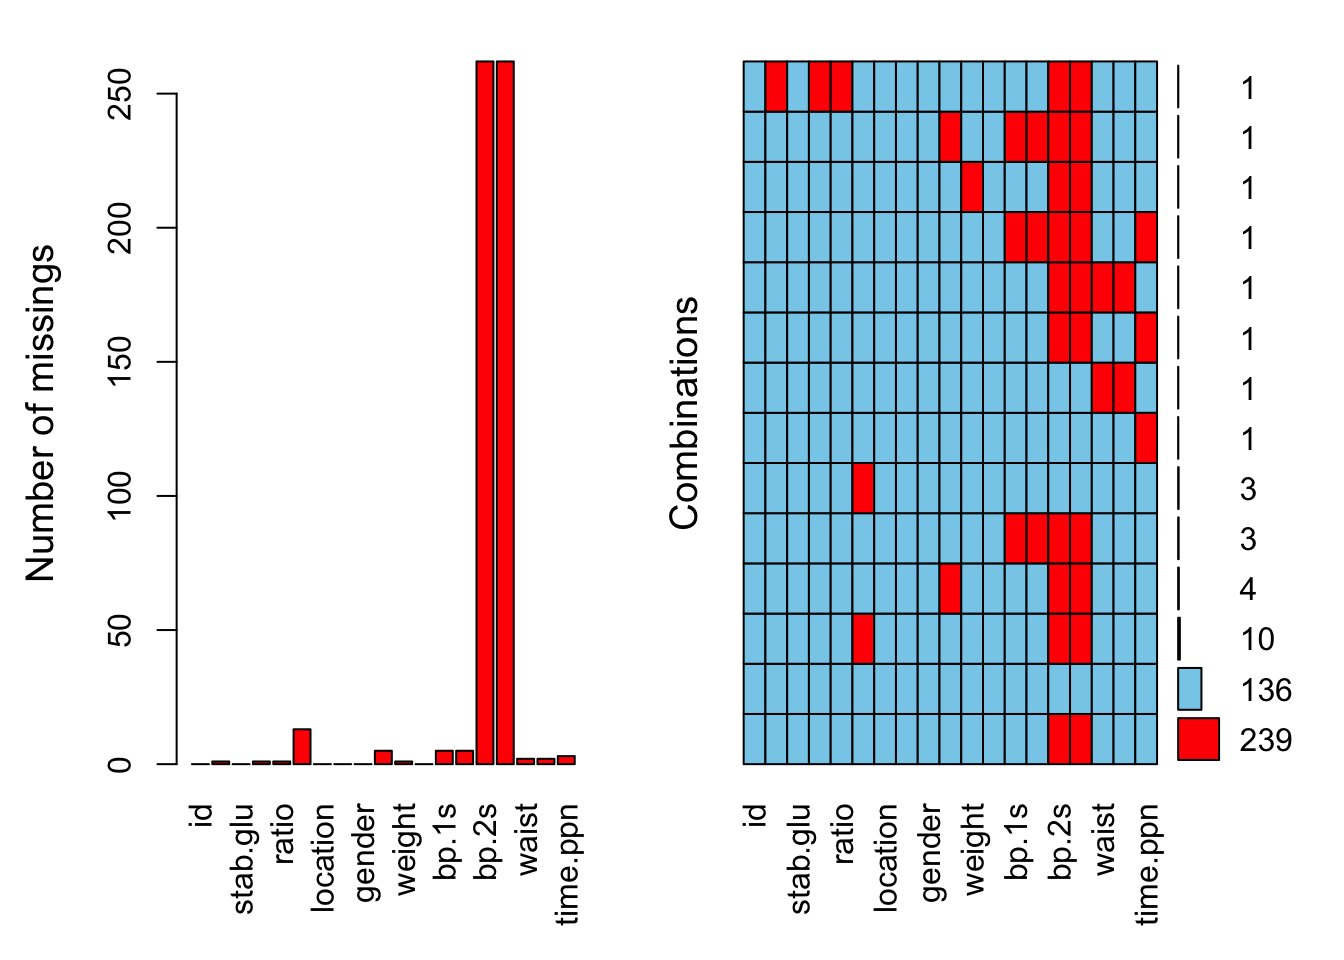
\includegraphics{main_files/figure-latex/unnamed-chunk-54-1.pdf} Siit on
näha, et kui me viskame välja 2 tulpa ja seejärel kõik read, mis
sisaldavad NA-sid, kaotame me u 20 rida 380-st, mis ei ole suur kaotus.

Kui palju ridu, milles on 0 NA-d? Mitu \% kõikidest ridadest?

\begin{Shaded}
\begin{Highlighting}[]
\NormalTok{nrows <-}\StringTok{ }\KeywordTok{nrow}\NormalTok{(diabetes)}
\NormalTok{  ncomplete <-}\StringTok{ }\KeywordTok{sum}\NormalTok{(}\KeywordTok{complete.cases}\NormalTok{(diabetes))}
\NormalTok{  ncomplete }\CommentTok{#136}
\end{Highlighting}
\end{Shaded}

\begin{verbatim}
## [1] 136
\end{verbatim}

\begin{Shaded}
\begin{Highlighting}[]
\NormalTok{  ncomplete}\OperatorTok{/}\NormalTok{nrows }\CommentTok{#34%}
\end{Highlighting}
\end{Shaded}

\begin{verbatim}
## [1] 0.337469
\end{verbatim}

Mitu NA-d igas tulbas?

\begin{Shaded}
\begin{Highlighting}[]
 \KeywordTok{sapply}\NormalTok{(diabetes, }\ControlFlowTok{function}\NormalTok{(x) }\KeywordTok{sum}\NormalTok{(}\KeywordTok{is.na}\NormalTok{(x))) }
\end{Highlighting}
\end{Shaded}

\begin{verbatim}
##       id     chol stab.glu      hdl    ratio    glyhb location      age 
##        0        1        0        1        1       13        0        0 
##   gender   height   weight    frame    bp.1s    bp.1d    bp.2s    bp.2d 
##        0        5        1        0        5        5      262      262 
##    waist      hip time.ppn 
##        2        2        3
\end{verbatim}

ploti NAd punasega igale tabeli reale ja tulbale mida tumedam halli toon
seda suurem number selle tulba kontekstis

\begin{Shaded}
\begin{Highlighting}[]
\NormalTok{VIM}\OperatorTok{::}\KeywordTok{matrixplot}\NormalTok{(diabetes) }
\end{Highlighting}
\end{Shaded}

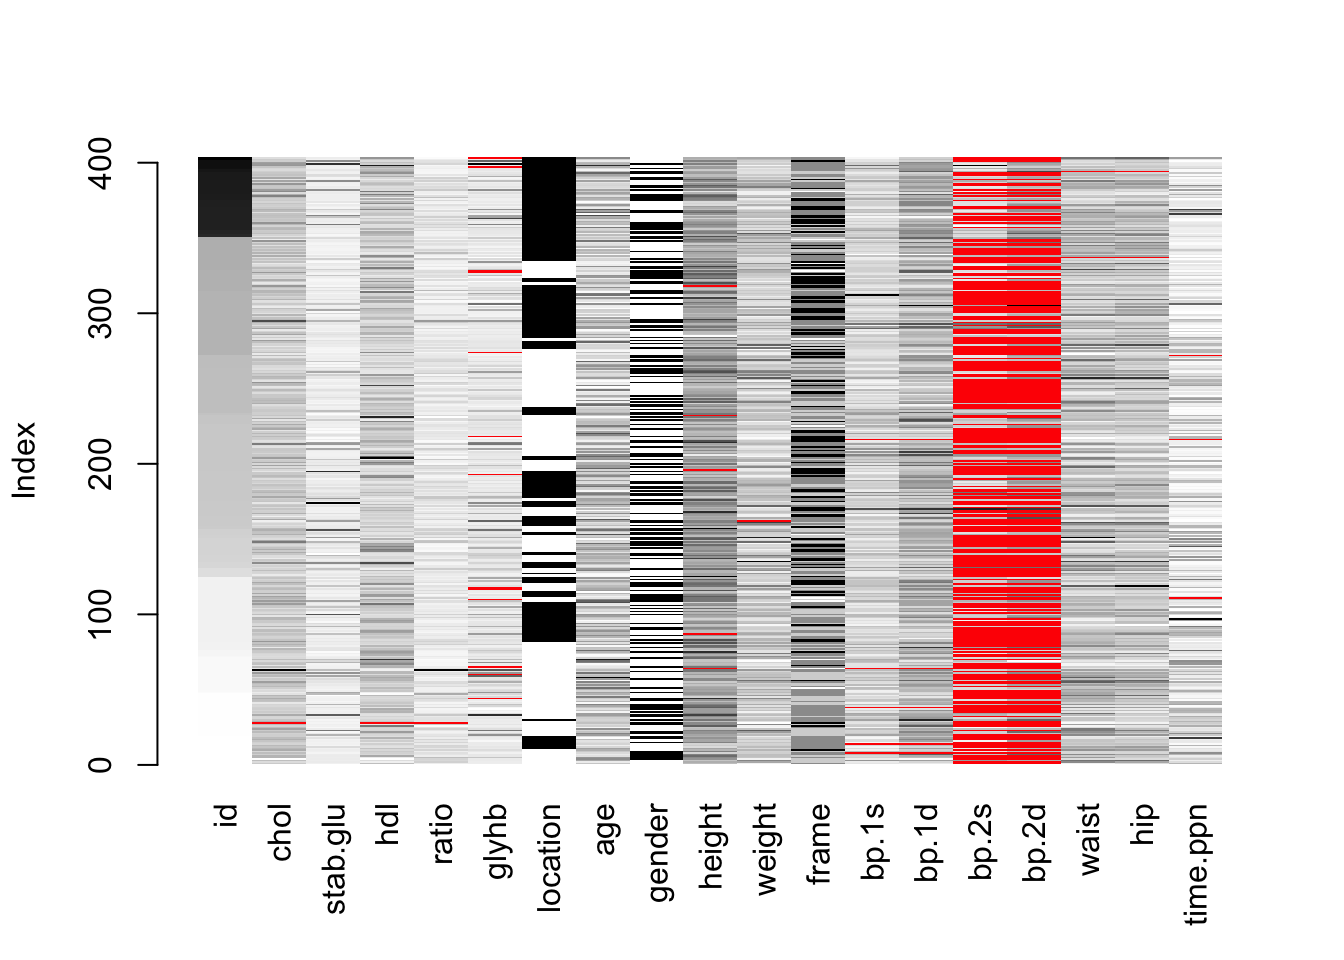
\includegraphics{main_files/figure-latex/unnamed-chunk-57-1.pdf}

kuidas rekodeerida NA-d näiteks 0-ks

\begin{Shaded}
\begin{Highlighting}[]
\NormalTok{df[}\KeywordTok{is.na}\NormalTok{(df)] <-}\StringTok{ }\DecValTok{0}
\NormalTok{df[}\KeywordTok{is.na}\NormalTok{(df)] <-}\StringTok{ "other"}
\NormalTok{df[df }\OperatorTok{==}\StringTok{ }\DecValTok{0}\NormalTok{] <-}\StringTok{ }\OtherTok{NA} \CommentTok{#teeb vastupidi 0-d NA-deks}
\end{Highlighting}
\end{Shaded}

Pane tähele, et NA tähistamine ei käi character vectorina vaid
dedikeeritud is.na() funktsiooniga.

\subsection{4. Matrix - numbriraam}\label{matrix---numbriraam}

Maatriks koosneb ühepikkustest vektoritest, mis sisaldavad ainult
numbreid. Enamasti me ei kasuta maatrikseid, vaid andmeraame. Tip: me
saame sageli andmeraami maatriksina kasutada kui me viskame sealt välja
mitte-numbrilised tulbad.

Aga saame ka andmeraame konverteerida otse maatriksiks (ja tagasi).
Vahest läheb seda vaja, eriti bioconductori funktsioonidega.

\begin{Shaded}
\begin{Highlighting}[]
\NormalTok{fruits <-}\StringTok{ }\KeywordTok{as.matrix}\NormalTok{(fruits)}
\KeywordTok{class}\NormalTok{(fruits)}
\end{Highlighting}
\end{Shaded}

\section{Andmete tüübid}\label{andmete-tuubid}

\begin{itemize}
\tightlist
\item
  numeric / integer
\item
  logical -2 väärtust TRUE/FALSE
\item
  character
\item
  factor (ordered and unordered) - 2+ diskreetset väärtust, mis võivad
  olla järjestatud suuremast väiksemani (aga ei asu üksteisest võrdsel
  kaugusel). Faktoreid käsitleme põhjalikumalt hiljem.
\end{itemize}

Andmete tüüpe saab üksteiseks konverteerida as.factor(), as.numeric(),
as.character(), as.integer(), as.logical()

\section{Indekseerimine}\label{indekseerimine}

Igale vektori, listi, andmeraami ja maatriksi elemendile vastab
unikaalne postiindeks, mille abil saame just selle elemendi unikaalselt
indentifitseerida, välja võtta ja töödelda.

Seega on indeksi mõte väga lühikese käsuga välja võtta R-i objektide
üksikuid elemente.

R-s algab indeksi numeratsioon 1-st (mitte 0-st, nagu Pythonis).

\subsection{Vektorid ja nende indeksid on
ühe-dimensionaalsed}\label{vektorid-ja-nende-indeksid-on-uhe-dimensionaalsed}

\begin{Shaded}
\begin{Highlighting}[]
\NormalTok{my_vector <-}\StringTok{ }\DecValTok{2}\OperatorTok{:}\DecValTok{5} 
\NormalTok{my_vector}
\end{Highlighting}
\end{Shaded}

\begin{verbatim}
## [1] 2 3 4 5
\end{verbatim}

\begin{Shaded}
\begin{Highlighting}[]
\NormalTok{my_vector[}\DecValTok{1}\NormalTok{] }\CommentTok{#1. element ehk number 2}
\end{Highlighting}
\end{Shaded}

\begin{verbatim}
## [1] 2
\end{verbatim}

\begin{Shaded}
\begin{Highlighting}[]
\NormalTok{my_vector[}\KeywordTok{c}\NormalTok{(}\DecValTok{1}\NormalTok{,}\DecValTok{3}\NormalTok{)] }\CommentTok{#1. ja 3. element }
\end{Highlighting}
\end{Shaded}

\begin{verbatim}
## [1] 2 4
\end{verbatim}

\begin{Shaded}
\begin{Highlighting}[]
\NormalTok{my_vector[}\OperatorTok{-}\DecValTok{1}\NormalTok{] }\CommentTok{#kõik elemendid, v.a. element number 1}
\end{Highlighting}
\end{Shaded}

\begin{verbatim}
## [1] 3 4 5
\end{verbatim}

\begin{Shaded}
\begin{Highlighting}[]
\NormalTok{my_vector[}\KeywordTok{c}\NormalTok{(}\OperatorTok{-}\DecValTok{1}\NormalTok{, }\OperatorTok{-}\DecValTok{3}\NormalTok{)] }\CommentTok{#kõik elemendid, v.a. element number 1 ja 3}
\end{Highlighting}
\end{Shaded}

\begin{verbatim}
## [1] 3 5
\end{verbatim}

\begin{Shaded}
\begin{Highlighting}[]
\NormalTok{my_vector[}\DecValTok{3}\OperatorTok{:}\DecValTok{5}\NormalTok{] }\CommentTok{#elemendid 3, 4 ja 5 (element 5 on määramata, seega NA)}
\end{Highlighting}
\end{Shaded}

\begin{verbatim}
## [1]  4  5 NA
\end{verbatim}

\begin{Shaded}
\begin{Highlighting}[]
\NormalTok{my_vector[}\OperatorTok{-}\NormalTok{(}\DecValTok{3}\OperatorTok{:}\KeywordTok{length}\NormalTok{(my_vector))] }\CommentTok{#1. ja 2. element}
\end{Highlighting}
\end{Shaded}

\begin{verbatim}
## [1] 2 3
\end{verbatim}

\subsection{andmeraamid ja maatriksid on kahe-dimensionaalsed, nagu ka
nende
indeksid}\label{andmeraamid-ja-maatriksid-on-kahe-dimensionaalsed-nagu-ka-nende-indeksid}

\textbf{2D indeksi kuju on {[}rea\_indeks, veeru\_indeks{]}}.

\begin{Shaded}
\begin{Highlighting}[]
\NormalTok{dat <-}\StringTok{ }\KeywordTok{tibble}\NormalTok{(}\DataTypeTok{colA =} \KeywordTok{c}\NormalTok{(}\StringTok{"a"}\NormalTok{, }\StringTok{"b"}\NormalTok{, }\StringTok{"c"}\NormalTok{), }\DataTypeTok{colB =} \KeywordTok{c}\NormalTok{(}\DecValTok{1}\NormalTok{, }\DecValTok{2}\NormalTok{, }\DecValTok{3}\NormalTok{))}
\NormalTok{dat}
\CommentTok{# üks andmepunkt: 1 rida, 2. veerg}
\NormalTok{dat[}\DecValTok{1}\NormalTok{, }\DecValTok{2}\NormalTok{]}
\CommentTok{# 1. rida, kõik veerud}
\NormalTok{dat[}\DecValTok{1}\NormalTok{, ]}
\CommentTok{# 2. veerg, kõik read}
\NormalTok{dat[, }\DecValTok{2}\NormalTok{]}
\CommentTok{# kõik read peale 1.}
\NormalTok{dat[}\OperatorTok{-}\DecValTok{1}\NormalTok{, ]}
\CommentTok{# viskab välja 2. veeru}
\NormalTok{dat[, }\OperatorTok{-}\DecValTok{2}\NormalTok{]}
\CommentTok{# 2 andmepunkti: 2. rida, 1. ja 2. veerg}
\NormalTok{dat[}\DecValTok{2}\NormalTok{, }\DecValTok{1}\OperatorTok{:}\DecValTok{2}\NormalTok{]}
\CommentTok{# 2 andmepunkti: 2. rida, 3. ja 4. veerg}
\NormalTok{dat[}\DecValTok{2}\NormalTok{, }\KeywordTok{c}\NormalTok{(}\DecValTok{1}\NormalTok{, }\DecValTok{2}\NormalTok{)]}
\CommentTok{#viskab välja 1. ja 2. rea}
\NormalTok{dat[}\OperatorTok{-}\KeywordTok{c}\NormalTok{(}\DecValTok{1}\NormalTok{, }\DecValTok{2}\NormalTok{), ]}
\CommentTok{#veerg nimega colB, output on erandina vektor!}
\NormalTok{dat}\OperatorTok{$}\NormalTok{colB}
\end{Highlighting}
\end{Shaded}

Kui me indekseerimisega tibblest veeru ehk vektori välja võtame, on
output class: tibble. Kui me teeme sama data frame-st, siis on output
class: vector.

Nüüd veidi keerulisemad konstruktsioonid, mis võimaldavad tabeli ühe
kindla veeru väärtusi välja tõmmata teise veeru väärtuste järgi
filteerides. Püüdke sellest koodist aru saada, et te hiljem ära
tunneksite, kui midagi sellist vastu tuleb. Õnneks ei ole teil endil
vaja sellist koodi kirjutada, me õpetame teile varsti lihtsama filtri
meetodi.

\begin{Shaded}
\begin{Highlighting}[]
\NormalTok{dat <-}\StringTok{ }\KeywordTok{tibble}\NormalTok{(}\DataTypeTok{colA =} \KeywordTok{c}\NormalTok{(}\StringTok{"a"}\NormalTok{, }\StringTok{"b"}\NormalTok{, }\StringTok{"c"}\NormalTok{), }\DataTypeTok{colB =} \KeywordTok{c}\NormalTok{(}\DecValTok{1}\NormalTok{, }\DecValTok{2}\NormalTok{, }\DecValTok{3}\NormalTok{))}
\NormalTok{dat}\OperatorTok{$}\NormalTok{colB[dat}\OperatorTok{$}\NormalTok{colA }\OperatorTok{!=}\StringTok{ "a"}\NormalTok{ ] }\CommentTok{#jätab sisse kõik vektori colB väärtused, kus samas tabeli reas olev colA väärtus ei ole "a". output on vektor! }
\end{Highlighting}
\end{Shaded}

\begin{verbatim}
## [1] 2 3
\end{verbatim}

\begin{Shaded}
\begin{Highlighting}[]
\NormalTok{dat}\OperatorTok{$}\NormalTok{colA[dat}\OperatorTok{$}\NormalTok{colB }\OperatorTok{>}\StringTok{ }\DecValTok{1}\NormalTok{] }\CommentTok{#jätab sisse kõik vektori colA väärtused, kus samas tabeli reas olev colB väärtus >1. output on vektor. }
\end{Highlighting}
\end{Shaded}

\begin{verbatim}
## [1] "b" "c"
\end{verbatim}

\subsection{litside indeksid on
kolme-dimensionaalsed}\label{litside-indeksid-on-kolme-dimensionaalsed}

\textbf{Listi indekseerimisel kasutame kahte sorti nurksulge, {[} {]} ja
{[}{[} {]}{]}, mis töötavad erinevalt}.

Kui listi vaadata nagu objektide vanglat, siis kaksiksulgude {[}{[}
{]}{]} abil on võimalik üksikuid objekte vanglast välja päästa nii, et
taastub nende algne kuju ehk class. (Vorm list\_name\$object\_name
töötab samamoodi kui kaksiksulud.) Seevastu üksiksulud {[} {]} tekitavad
uue listi, kus on säilinud osad algse listi elemendid, ehk uue vangla
vähemate vangidega.

\begin{quote}
Kaksiksulud {[}{[} {]}{]} päästavad listist välja ühe elemendi ja
taastavad selle algse class-i (data.frame, vektor, list jms); Üksiksulud
{[} {]} võtavad algsest listist välja teie poolt valitud elemendid aga
jätavad uue objekti ikka listi kujule.
\end{quote}

\begin{Shaded}
\begin{Highlighting}[]
\NormalTok{my_list <-}\StringTok{ }\KeywordTok{list}\NormalTok{(}\DataTypeTok{a=}\KeywordTok{tibble}\NormalTok{(}\DataTypeTok{colA=}\KeywordTok{c}\NormalTok{(}\StringTok{"A"}\NormalTok{, }\StringTok{"B"}\NormalTok{), }\DataTypeTok{colB=}\KeywordTok{c}\NormalTok{(}\DecValTok{1}\NormalTok{,}\DecValTok{2}\NormalTok{)), }\DataTypeTok{b=}\KeywordTok{c}\NormalTok{(}\DecValTok{1}\NormalTok{, }\OtherTok{NA}\NormalTok{, }\StringTok{"s"}\NormalTok{))}
\CommentTok{#this list has two elements, a df called "a" and a character vector called "b".}
\KeywordTok{str}\NormalTok{(my_list)}
\end{Highlighting}
\end{Shaded}

\begin{verbatim}
## List of 2
##  $ a:Classes 'tbl_df', 'tbl' and 'data.frame':   2 obs. of  2 variables:
##   ..$ colA: chr [1:2] "A" "B"
##   ..$ colB: num [1:2] 1 2
##  $ b: chr [1:3] "1" NA "s"
\end{verbatim}

Tõmbame listist välja tibble

\begin{Shaded}
\begin{Highlighting}[]
\NormalTok{my_tibble <-}\StringTok{ }\NormalTok{my_list[[}\DecValTok{1}\NormalTok{]] }\CommentTok{#class is df  --- we extracted a df from the list}
\NormalTok{my_tibble}
\end{Highlighting}
\end{Shaded}

\begin{verbatim}
## # A tibble: 2 x 2
##    colA  colB
##   <chr> <dbl>
## 1     A     1
## 2     B     2
\end{verbatim}

\begin{Shaded}
\begin{Highlighting}[]
\CommentTok{#my_list$a #sama asi: $ does the same thing as [[ ]]}
\end{Highlighting}
\end{Shaded}

See ei ole enam list

Nüüd võtame üksiksuluga listist välja 1. elemendi, mis on tibble, aga
output ei ole mitte tibble, vaid ikka list. Seekord ühe elemendiga, mis
on tibble.

\begin{Shaded}
\begin{Highlighting}[]
\NormalTok{aa <-}\StringTok{ }\NormalTok{my_list[}\DecValTok{1}\NormalTok{]}
\KeywordTok{str}\NormalTok{(aa)}
\end{Highlighting}
\end{Shaded}

\begin{verbatim}
## List of 1
##  $ a:Classes 'tbl_df', 'tbl' and 'data.frame':   2 obs. of  2 variables:
##   ..$ colA: chr [1:2] "A" "B"
##   ..$ colB: num [1:2] 1 2
\end{verbatim}

\begin{Shaded}
\begin{Highlighting}[]
\NormalTok{aa1 <-}\StringTok{ }\NormalTok{my_list}\OperatorTok{$}\NormalTok{a[}\DecValTok{2}\NormalTok{,] }\CommentTok{#class is df}
\NormalTok{aa1}
\end{Highlighting}
\end{Shaded}

\begin{verbatim}
## # A tibble: 1 x 2
##    colA  colB
##   <chr> <dbl>
## 1     B     2
\end{verbatim}

\begin{Shaded}
\begin{Highlighting}[]
\NormalTok{aa3 <-}\StringTok{ }\NormalTok{my_list[[}\DecValTok{1}\NormalTok{]][}\DecValTok{1}\NormalTok{,]}
\NormalTok{aa3}
\end{Highlighting}
\end{Shaded}

\begin{verbatim}
## # A tibble: 1 x 2
##    colA  colB
##   <chr> <dbl>
## 1     A     1
\end{verbatim}

Kõigepealt läksime kaksiksulgudega listi taseme võrra sisse ja võtsime
välja objekti my\_list 1. elemendi, tema algses tibble formaadis,
(indeksi 1. dimensioon). Seejärel korjame sealt välja 1. rea, tibble
formaati muutmata ja seega üksiksulgudes (indeksi 2. ja 3. dimensioon).

Pane tähele, et {[}{[} {]}{]} lubab ainult ühe elemendi korraga listist
välja päästa.

\section{Regular expression ja find \&
replace}\label{regular-expression-ja-find-replace}

Regular expression annab võimaluse lühidalt kirjeldada mitte-üheseid
otsinguparameetreid.

\begin{quote}
regular expression on string, mis kirjeldab mitut stringi
\end{quote}

A
\href{https://stat.ethz.ch/R-manual/R-devel/library/base/html/regex.html}{regular
expression}
\href{https://stat.ethz.ch/R-manual/R-devel/library/base/html/regex.html}{Regular
Expressions as used in R}

\begin{itemize}
\tightlist
\item
  Most characters, including all letters and digits, are regular
  expressions that match themselves.
\item
  \texttt{.} matches any single character.
\item
  You can refer also to a character class, which is a list of characters
  enclosed between \texttt{{[}} and \texttt{{]}}, e.g.
  \texttt{{[}{[}:alnum:{]}{]}} is same as \texttt{{[}A-z0-9{]}}.
\item
  Most common character classes:

  \begin{itemize}
  \tightlist
  \item
    \texttt{{[}:alnum:{]}} includes alphanumerics
    (\texttt{{[}:alpha:{]}} and \texttt{{[}:digit:{]}});
  \item
    \texttt{{[}:alpha:{]}}, includes alphabetic characters
    (\texttt{{[}:upper:{]}} and \texttt{{[}:lower:{]}} case);
  \item
    \texttt{{[}:punct:{]}} includes punctuation characters ! " \# \$ \%
    \& ' ( ) * + , - . / : ; \textless{} = \textgreater{} ? @ {[} ~{]}
    \^{} \_ ` ` \{ \textbar{} \} \textasciitilde{}.;
  \item
    \texttt{{[}:blank:{]}} includes space and tab; etc.
  \end{itemize}
\item
  The metacharacters in regular expressions are
  \texttt{.\ \textbackslash{}\ \textbar{}\ (\ )\ {[}\ \{\ \^{}\ \$\ *\ +\ ?},
  whether these have a special meaning depends on the context. When
  matching a metacharacter as a regular character, precede it with a
  double backslash \texttt{\textbackslash{}\textbackslash{}}.
\item
  Repetition quantifiers put after regex specify how many times regex is
  matched: \texttt{?}, optional, at most once; \texttt{*}, zero or more
  times; \texttt{+}, one or more times; \texttt{\{n\}}, n times;
  \texttt{\{n,\}}, n or more times; \texttt{\{n,m\}}, n to m times.
\item
  \^{} anchors the regular expression to the start of the string.
\item
  \$ anchors the the regular expression to end of the string.
\end{itemize}

\subsubsection{Common operations with regular
expressions}\label{common-operations-with-regular-expressions}

\begin{itemize}
\tightlist
\item
  Locate a pattern match (positions)
\item
  Extract a matched pattern
\item
  Identify a match to a pattern
\item
  Replace a matched pattern
\end{itemize}

\subsubsection{Find and replace}\label{find-and-replace}

\begin{Shaded}
\begin{Highlighting}[]
\KeywordTok{library}\NormalTok{(stringr)}
\NormalTok{x<-}\StringTok{ }\KeywordTok{c}\NormalTok{(}\StringTok{"apple"}\NormalTok{, }\StringTok{"ananas"}\NormalTok{, }\StringTok{"banana"}\NormalTok{)}

\CommentTok{#replaces all a-s at the beginning of strings with e-s}
\KeywordTok{str_replace}\NormalTok{(x, }\StringTok{"^a"}\NormalTok{, }\StringTok{"e"}\NormalTok{) }
\end{Highlighting}
\end{Shaded}

\begin{verbatim}
## [1] "epple"  "enanas" "banana"
\end{verbatim}

\begin{Shaded}
\begin{Highlighting}[]
\CommentTok{# str_replace only replaces at the first occurence at each string}
\KeywordTok{str_replace}\NormalTok{(x, }\StringTok{"a"}\NormalTok{, }\StringTok{"e"}\NormalTok{) }
\end{Highlighting}
\end{Shaded}

\begin{verbatim}
## [1] "epple"  "enanas" "benana"
\end{verbatim}

\begin{Shaded}
\begin{Highlighting}[]
\CommentTok{#str_replace_all replaces all a-s anywhere in the strings}
\KeywordTok{str_replace_all}\NormalTok{(x, }\StringTok{"a"}\NormalTok{, }\StringTok{"e"}\NormalTok{) }
\end{Highlighting}
\end{Shaded}

\begin{verbatim}
## [1] "epple"  "enenes" "benene"
\end{verbatim}

\begin{Shaded}
\begin{Highlighting}[]
\CommentTok{#replaces a and the following character at the end of string with nothing (i.e. deletes 2 chars)}
\KeywordTok{str_replace}\NormalTok{(x, }\StringTok{"a.$"}\NormalTok{, }\StringTok{""}\NormalTok{)}
\end{Highlighting}
\end{Shaded}

\begin{verbatim}
## [1] "apple"  "anan"   "banana"
\end{verbatim}

\begin{Shaded}
\begin{Highlighting}[]
\CommentTok{#replaces a-s or s-s at the end of string with e-s}
\KeywordTok{str_replace}\NormalTok{(x, }\StringTok{"(a|s)$"}\NormalTok{, }\StringTok{"e"}\NormalTok{)}
\end{Highlighting}
\end{Shaded}

\begin{verbatim}
## [1] "apple"  "ananae" "banane"
\end{verbatim}

\begin{Shaded}
\begin{Highlighting}[]
\CommentTok{#replaces a-s or s-s anywhere in the string with e-s}
\KeywordTok{str_replace_all}\NormalTok{(x, }\StringTok{"a|s"}\NormalTok{, }\StringTok{"e"}\NormalTok{)}
\end{Highlighting}
\end{Shaded}

\begin{verbatim}
## [1] "epple"  "enenee" "benene"
\end{verbatim}

\begin{Shaded}
\begin{Highlighting}[]
\CommentTok{#remove all numbers. }
\NormalTok{y<-}\KeywordTok{c}\NormalTok{(}\StringTok{"as1"}\NormalTok{, }\StringTok{"2we3w"}\NormalTok{, }\StringTok{"3e"}\NormalTok{)}
\KeywordTok{str_replace_all}\NormalTok{(y, }\StringTok{"}\CharTok{\textbackslash{}\textbackslash{}}\StringTok{d"}\NormalTok{, }\StringTok{""}\NormalTok{) }
\end{Highlighting}
\end{Shaded}

\begin{verbatim}
## [1] "as"  "wew" "e"
\end{verbatim}

\begin{Shaded}
\begin{Highlighting}[]
\CommentTok{#remove everything, except numbers. }
\KeywordTok{str_replace_all}\NormalTok{(y, }\StringTok{"[A-Za-z_]"}\NormalTok{, }\StringTok{""}\NormalTok{) }
\end{Highlighting}
\end{Shaded}

\begin{verbatim}
## [1] "1"  "23" "3"
\end{verbatim}

\begin{Shaded}
\begin{Highlighting}[]
\NormalTok{x<-}\StringTok{ }\KeywordTok{c}\NormalTok{(}\StringTok{"apple"}\NormalTok{, }\StringTok{"apple pie"}\NormalTok{)}
\KeywordTok{str_replace_all}\NormalTok{(x, }\StringTok{"^apple$"}\NormalTok{,}\StringTok{"m"}\NormalTok{) }\CommentTok{#To force to only match a complete string:}
\end{Highlighting}
\end{Shaded}

\begin{verbatim}
## [1] "m"         "apple pie"
\end{verbatim}

\begin{Shaded}
\begin{Highlighting}[]
\KeywordTok{str_replace_all}\NormalTok{(x, }\StringTok{"}\CharTok{\textbackslash{}\textbackslash{}}\StringTok{s"}\NormalTok{,}\StringTok{"_"}\NormalTok{) }\CommentTok{#space to _}
\end{Highlighting}
\end{Shaded}

\begin{verbatim}
## [1] "apple"     "apple_pie"
\end{verbatim}

\begin{Shaded}
\begin{Highlighting}[]
\KeywordTok{str_replace_all}\NormalTok{(x, }\StringTok{"[apl]"}\NormalTok{,}\StringTok{"_"}\NormalTok{) }\CommentTok{#a or p or l to _}
\end{Highlighting}
\end{Shaded}

\begin{verbatim}
## [1] "____e"     "____e _ie"
\end{verbatim}

\begin{Shaded}
\begin{Highlighting}[]
\KeywordTok{str_replace_all}\NormalTok{(x, }\StringTok{"[ap|p.e]"}\NormalTok{,}\StringTok{"_"}\NormalTok{) }\CommentTok{# ap or p.e to _}
\end{Highlighting}
\end{Shaded}

\begin{verbatim}
## [1] "___l_"     "___l_ _i_"
\end{verbatim}

\textbf{patterns that match more than one character:}

\begin{Shaded}
\begin{Highlighting}[]
\NormalTok{. (dot)}\OperatorTok{:}\StringTok{ }\NormalTok{any character apart from a newline.}

\NormalTok{\textbackslash{}\textbackslash{}d}\OperatorTok{:}\StringTok{ }\NormalTok{any digit.}

\NormalTok{\textbackslash{}\textbackslash{}s}\OperatorTok{:}\StringTok{ }\NormalTok{any }\KeywordTok{whitespace}\NormalTok{ (space, tab, newline).}

\NormalTok{\textbackslash{}[abc]}\OperatorTok{:}\StringTok{ }\NormalTok{match a, b, or c.}

\NormalTok{\textbackslash{}[}\OperatorTok{!}\NormalTok{abc]}\OperatorTok{:}\StringTok{ }\NormalTok{match anything except a, b, or c.}

\NormalTok{To create a regular expression containing \textbackslash{}d or \textbackslash{}s, you???ll need to escape the \textbackslash{} }\ControlFlowTok{for}\NormalTok{ the string, so you will type }\StringTok{"}\CharTok{\textbackslash{}\textbackslash{}\textbackslash{}\textbackslash{}}\StringTok{d"}\NormalTok{ or }\StringTok{"}\CharTok{\textbackslash{}\textbackslash{}\textbackslash{}\textbackslash{}}\StringTok{s"}\NormalTok{.}

\NormalTok{abc}\OperatorTok{|}\NormalTok{d..f will match either }\StringTok{"abc"}\NormalTok{, or }\StringTok{"deaf"}\NormalTok{. }
\end{Highlighting}
\end{Shaded}

\section{Tidyverse}\label{tidyverse}

Tidyverse on väike osa R-i ökosüsteemist, kus kehtivad omad reeglid.
Tidyverse raamatukogud lähtuvad ühtsest filosoofiast ja töötavad hästi
koos. Tidyverse algab andmetabeli struktuurist ja selle funktsioonid
võtavad reeglina sisse õige struktuuriga tibble ja väljastavad samuti
tibble, mis sobib hästi järgmise tidyverse funktsiooni sisendiks. Seega
on tidyverse hästi sobiv läbi torude \%\textgreater{}\% laskmiseks.
Tidyversiga sobib hästi kokku ka ggplot2 graafikasüsteem.

\subsection{Tidy tabeli struktuur}\label{tidy-tabeli-struktuur}

\begin{itemize}
\tightlist
\item
  \textbf{väärtus} (\emph{value}) --- ühe mõõtmise tulemus (183 cm)
\item
  \textbf{muutuja} (\emph{variable}) --- see, mida sa mõõdad (pikkus)
  või faktor (sex)
\item
  \textbf{andmepunkt} (\emph{observation}) --- väärtused, mis mõõdeti
  samal katsetingimusel (1. subjekti pikkus ja kaal 3h ajapunktis)
\item
  \textbf{vaatlusühik} (\emph{unit of measurement}) --- keda mõõdeti
  (subjekt nr 1)
\item
  \textbf{vaatlusühiku tüüp} --- inimene, hiir, jt
\end{itemize}

\begin{quote}
vaatlusühiku tüüp = tabel
\end{quote}

\begin{quote}
muutuja = veerg
\end{quote}

\begin{quote}
andmepunkt = rida
\end{quote}

\begin{quote}
vaatlusühikute koodid on kõik koos ühes veerus
\end{quote}

Veergude järjekord tabelis on 1. vaatlusühik, 2. faktor, mis annab
katse-kontrolli erisuse, 3. kõik see, mida otse ei mõõdetud (sex, batch
nr, etc.), 4. numbritega veerud (iga muutuja kohta üks veerg)

\begin{verbatim}
## # A tibble: 2 x 6
##   subject    drug   sex  time length weigth
##     <chr>   <chr> <chr> <dbl>  <dbl>  <dbl>
## 1       1     exp     F     3    168     88
## 2       2 placebo     M     3    176     91
\end{verbatim}

Nii näeb välja tidy tibble. Kõik analüüsil vajalikud parameetrid tuleks
siia tabelisse veeru kaupa sisse tuua. Näiteks, kui mõõtmised on
sooritatud erinevates keskustes erinevate inimeste poolt kasutades sama
ravimi erinevaid preparaate, oleks hea siia veel 3 veergu lisada
(center, experimenter, batch).

\subsection{Tabeli dimensioonide muutmine (pikk ja lai
formaat)}\label{tabeli-dimensioonide-muutmine-pikk-ja-lai-formaat}

Väga oluline osa tidyverses töötamisest on tabelite pika ja laia
formaadi vahel viimine.

See on laias formaadis tabel df, mis ei ole tidy

\begin{verbatim}
## # A tibble: 3 x 5
##   subject   sex control experiment_1 experiment_2
##     <chr> <chr>   <dbl>        <dbl>        <dbl>
## 1     Tim     M      23           34           40
## 2     Ann     F      31           38           42
## 3    Jill     F      30           36           44
\end{verbatim}

Kõigepealt pikka formaati. key ja value argumendid on ainult uute
veergude nimetamiseks, oluline on 3:ncol(dat) argument, mis ütleb, et
``kogu kokku veerud alates 3. veerust''. Alternatiivne viis seda öelda:
c(-subject, -sex).

\begin{Shaded}
\begin{Highlighting}[]
\NormalTok{dat_lng <-}\StringTok{ }\KeywordTok{gather}\NormalTok{(dat, }\DataTypeTok{key =}\NormalTok{ experiment, }\DataTypeTok{value =}\NormalTok{ value, }\DecValTok{3}\OperatorTok{:}\KeywordTok{ncol}\NormalTok{(dat))}
\CommentTok{# df_l3<-df %>% gather(experiment, value, 3:ncol(df)) works as well.}
\CommentTok{#df_l4<-df %>% gather(experiment, value, c(-subject, -sex)) works as well}
\NormalTok{dat_lng}
\end{Highlighting}
\end{Shaded}

\begin{verbatim}
## # A tibble: 9 x 4
##   subject   sex   experiment value
##     <chr> <chr>        <chr> <dbl>
## 1     Tim     M      control    23
## 2     Ann     F      control    31
## 3    Jill     F      control    30
## 4     Tim     M experiment_1    34
## 5     Ann     F experiment_1    38
## 6    Jill     F experiment_1    36
## 7     Tim     M experiment_2    40
## 8     Ann     F experiment_2    42
## 9    Jill     F experiment_2    44
\end{verbatim}

Paneme selle tagasi algsesse laia formaati: ?spread

\begin{Shaded}
\begin{Highlighting}[]
\KeywordTok{spread}\NormalTok{(dat_lng, }\DataTypeTok{key =}\NormalTok{ experiment, }\DataTypeTok{value =}\NormalTok{ value)}
\end{Highlighting}
\end{Shaded}

\begin{verbatim}
## # A tibble: 3 x 5
##   subject   sex control experiment_1 experiment_2
## *   <chr> <chr>   <dbl>        <dbl>        <dbl>
## 1     Ann     F      31           38           42
## 2    Jill     F      30           36           44
## 3     Tim     M      23           34           40
\end{verbatim}

key viitab pika tabeli veerule, mille väärtustest tulevad laias tabelis
uute veergude nimed. value viitab pika tabeli veerule, kust võetakse
arvud, mis uues laias tabelis uute veergude vahel laiali jagatakse.

\subsubsection{Tibble transpose --- read veergudeks ja
vastupidi}\label{tibble-transpose-read-veergudeks-ja-vastupidi}

\begin{Shaded}
\begin{Highlighting}[]
\NormalTok{dat <-}\StringTok{ }\KeywordTok{tibble}\NormalTok{(}\DataTypeTok{a =} \KeywordTok{c}\NormalTok{(}\StringTok{"tim"}\NormalTok{, }\StringTok{"tom"}\NormalTok{, }\StringTok{"jill"}\NormalTok{), }\DataTypeTok{b1 =} \KeywordTok{c}\NormalTok{(}\DecValTok{1}\NormalTok{, }\DecValTok{2}\NormalTok{, }\DecValTok{3}\NormalTok{), }\DataTypeTok{b2 =} \KeywordTok{c}\NormalTok{(}\DecValTok{4}\NormalTok{, }\DecValTok{5}\NormalTok{, }\DecValTok{6}\NormalTok{))}
\NormalTok{dat}
\end{Highlighting}
\end{Shaded}

\begin{verbatim}
## # A tibble: 3 x 3
##       a    b1    b2
##   <chr> <dbl> <dbl>
## 1   tim     1     4
## 2   tom     2     5
## 3  jill     3     6
\end{verbatim}

Me kasutame selleks maatriksarvutuse funktsiooni t() --- transpose. See
võtab sisse ainult numbrilisi veerge, seega anname talle ette df miinus
1. veerg, mille sisu me konverteerime uue tablei veerunimedeks.

\begin{Shaded}
\begin{Highlighting}[]
\NormalTok{dat1 <-}\StringTok{ }\KeywordTok{t}\NormalTok{(dat[,}\OperatorTok{-}\DecValTok{1}\NormalTok{])}
\KeywordTok{colnames}\NormalTok{(dat1) <-}\StringTok{ }\NormalTok{dat}\OperatorTok{$}\NormalTok{a}
\NormalTok{dat1}
\end{Highlighting}
\end{Shaded}

\begin{verbatim}
##    tim tom jill
## b1   1   2    3
## b2   4   5    6
\end{verbatim}

\section{dplyr-i 5 verbi}\label{dplyr-i-5-verbi}

Need tuleb teil omale pähe ajada sest nende 5 verbiga (pluss gather ja
spread) saab lihtsalt teha 90\% andmeväänamisest, mida teil elus vaja
läheb. NB! Check the data wrangling cheatsheet and dplyr help for
further details. dplyr laetakse koos tidyverse-ga automaatselt teie
workspace.

\subsection{\texorpdfstring{\texttt{select()}
columns}{select() columns}}\label{select-columns}

\texttt{select()} selects, renames, and re-orders columns.

Select columns from sex to value:

\begin{Shaded}
\begin{Highlighting}[]
\NormalTok{iris}
\KeywordTok{select}\NormalTok{(iris, Petal.Length}\OperatorTok{:}\NormalTok{Species)}
\KeywordTok{select}\NormalTok{(iris, }\OperatorTok{-}\NormalTok{(Petal.Length}\OperatorTok{:}\NormalTok{Species)) }\CommentTok{#selects everything, except those cols}
\end{Highlighting}
\end{Shaded}

To select 3 columns and rename \emph{subject} to \emph{SUBJ} and put
liik as the 1st col:

\begin{Shaded}
\begin{Highlighting}[]
\KeywordTok{select}\NormalTok{(iris, }\DataTypeTok{liik =}\NormalTok{ Species, Sepal.Length, Sepal.Width )}
\end{Highlighting}
\end{Shaded}

\begin{verbatim}
##           liik Sepal.Length Sepal.Width
## 1       setosa          5.1         3.5
## 2       setosa          4.9         3.0
## 3       setosa          4.7         3.2
## 4       setosa          4.6         3.1
## 5       setosa          5.0         3.6
## 6       setosa          5.4         3.9
## 7       setosa          4.6         3.4
## 8       setosa          5.0         3.4
## 9       setosa          4.4         2.9
## 10      setosa          4.9         3.1
## 11      setosa          5.4         3.7
## 12      setosa          4.8         3.4
## 13      setosa          4.8         3.0
## 14      setosa          4.3         3.0
## 15      setosa          5.8         4.0
## 16      setosa          5.7         4.4
## 17      setosa          5.4         3.9
## 18      setosa          5.1         3.5
## 19      setosa          5.7         3.8
## 20      setosa          5.1         3.8
## 21      setosa          5.4         3.4
## 22      setosa          5.1         3.7
## 23      setosa          4.6         3.6
## 24      setosa          5.1         3.3
## 25      setosa          4.8         3.4
## 26      setosa          5.0         3.0
## 27      setosa          5.0         3.4
## 28      setosa          5.2         3.5
## 29      setosa          5.2         3.4
## 30      setosa          4.7         3.2
## 31      setosa          4.8         3.1
## 32      setosa          5.4         3.4
## 33      setosa          5.2         4.1
## 34      setosa          5.5         4.2
## 35      setosa          4.9         3.1
## 36      setosa          5.0         3.2
## 37      setosa          5.5         3.5
## 38      setosa          4.9         3.6
## 39      setosa          4.4         3.0
## 40      setosa          5.1         3.4
## 41      setosa          5.0         3.5
## 42      setosa          4.5         2.3
## 43      setosa          4.4         3.2
## 44      setosa          5.0         3.5
## 45      setosa          5.1         3.8
## 46      setosa          4.8         3.0
## 47      setosa          5.1         3.8
## 48      setosa          4.6         3.2
## 49      setosa          5.3         3.7
## 50      setosa          5.0         3.3
## 51  versicolor          7.0         3.2
## 52  versicolor          6.4         3.2
## 53  versicolor          6.9         3.1
## 54  versicolor          5.5         2.3
## 55  versicolor          6.5         2.8
## 56  versicolor          5.7         2.8
## 57  versicolor          6.3         3.3
## 58  versicolor          4.9         2.4
## 59  versicolor          6.6         2.9
## 60  versicolor          5.2         2.7
## 61  versicolor          5.0         2.0
## 62  versicolor          5.9         3.0
## 63  versicolor          6.0         2.2
## 64  versicolor          6.1         2.9
## 65  versicolor          5.6         2.9
## 66  versicolor          6.7         3.1
## 67  versicolor          5.6         3.0
## 68  versicolor          5.8         2.7
## 69  versicolor          6.2         2.2
## 70  versicolor          5.6         2.5
## 71  versicolor          5.9         3.2
## 72  versicolor          6.1         2.8
## 73  versicolor          6.3         2.5
## 74  versicolor          6.1         2.8
## 75  versicolor          6.4         2.9
## 76  versicolor          6.6         3.0
## 77  versicolor          6.8         2.8
## 78  versicolor          6.7         3.0
## 79  versicolor          6.0         2.9
## 80  versicolor          5.7         2.6
## 81  versicolor          5.5         2.4
## 82  versicolor          5.5         2.4
## 83  versicolor          5.8         2.7
## 84  versicolor          6.0         2.7
## 85  versicolor          5.4         3.0
## 86  versicolor          6.0         3.4
## 87  versicolor          6.7         3.1
## 88  versicolor          6.3         2.3
## 89  versicolor          5.6         3.0
## 90  versicolor          5.5         2.5
## 91  versicolor          5.5         2.6
## 92  versicolor          6.1         3.0
## 93  versicolor          5.8         2.6
## 94  versicolor          5.0         2.3
## 95  versicolor          5.6         2.7
## 96  versicolor          5.7         3.0
## 97  versicolor          5.7         2.9
## 98  versicolor          6.2         2.9
## 99  versicolor          5.1         2.5
## 100 versicolor          5.7         2.8
## 101  virginica          6.3         3.3
## 102  virginica          5.8         2.7
## 103  virginica          7.1         3.0
## 104  virginica          6.3         2.9
## 105  virginica          6.5         3.0
## 106  virginica          7.6         3.0
## 107  virginica          4.9         2.5
## 108  virginica          7.3         2.9
## 109  virginica          6.7         2.5
## 110  virginica          7.2         3.6
## 111  virginica          6.5         3.2
## 112  virginica          6.4         2.7
## 113  virginica          6.8         3.0
## 114  virginica          5.7         2.5
## 115  virginica          5.8         2.8
## 116  virginica          6.4         3.2
## 117  virginica          6.5         3.0
## 118  virginica          7.7         3.8
## 119  virginica          7.7         2.6
## 120  virginica          6.0         2.2
## 121  virginica          6.9         3.2
## 122  virginica          5.6         2.8
## 123  virginica          7.7         2.8
## 124  virginica          6.3         2.7
## 125  virginica          6.7         3.3
## 126  virginica          7.2         3.2
## 127  virginica          6.2         2.8
## 128  virginica          6.1         3.0
## 129  virginica          6.4         2.8
## 130  virginica          7.2         3.0
## 131  virginica          7.4         2.8
## 132  virginica          7.9         3.8
## 133  virginica          6.4         2.8
## 134  virginica          6.3         2.8
## 135  virginica          6.1         2.6
## 136  virginica          7.7         3.0
## 137  virginica          6.3         3.4
## 138  virginica          6.4         3.1
## 139  virginica          6.0         3.0
## 140  virginica          6.9         3.1
## 141  virginica          6.7         3.1
## 142  virginica          6.9         3.1
## 143  virginica          5.8         2.7
## 144  virginica          6.8         3.2
## 145  virginica          6.7         3.3
## 146  virginica          6.7         3.0
## 147  virginica          6.3         2.5
## 148  virginica          6.5         3.0
## 149  virginica          6.2         3.4
## 150  virginica          5.9         3.0
\end{verbatim}

To select all cols, except sex and value, and rename the \emph{subject}
col:

\begin{Shaded}
\begin{Highlighting}[]
\KeywordTok{select}\NormalTok{(iris, }\OperatorTok{-}\NormalTok{Sepal.Length, }\OperatorTok{-}\NormalTok{Sepal.Width, }\DataTypeTok{liik =}\NormalTok{ Species)}
\end{Highlighting}
\end{Shaded}

\textbf{helper functions you can use within select():}

starts\_with(``abc''): matches names that begin with ``abc.''

ends\_with(``xyz''): matches names that end with ``xyz.''

contains(``ijk''): matches names that contain ``ijk.''

matches(``(.)\textbackslash{}1''): selects variables that match a
regular expression. This one matches any variables that contain repeated
characters.

num\_range(``x'', 1:3) matches x1, x2 and x3.

\begin{Shaded}
\begin{Highlighting}[]
\NormalTok{iris <-}\StringTok{ }\KeywordTok{as_tibble}\NormalTok{(iris)}
\KeywordTok{select}\NormalTok{(iris, }\KeywordTok{starts_with}\NormalTok{(}\StringTok{"Petal"}\NormalTok{))}
\end{Highlighting}
\end{Shaded}

\begin{verbatim}
## # A tibble: 150 x 2
##    Petal.Length Petal.Width
##           <dbl>       <dbl>
##  1          1.4         0.2
##  2          1.4         0.2
##  3          1.3         0.2
##  4          1.5         0.2
##  5          1.4         0.2
##  6          1.7         0.4
##  7          1.4         0.3
##  8          1.5         0.2
##  9          1.4         0.2
## 10          1.5         0.1
## # ... with 140 more rows
\end{verbatim}

\begin{Shaded}
\begin{Highlighting}[]
\KeywordTok{select}\NormalTok{(iris, }\KeywordTok{ends_with}\NormalTok{(}\StringTok{"Width"}\NormalTok{))}
\end{Highlighting}
\end{Shaded}

\begin{verbatim}
## # A tibble: 150 x 2
##    Sepal.Width Petal.Width
##          <dbl>       <dbl>
##  1         3.5         0.2
##  2         3.0         0.2
##  3         3.2         0.2
##  4         3.1         0.2
##  5         3.6         0.2
##  6         3.9         0.4
##  7         3.4         0.3
##  8         3.4         0.2
##  9         2.9         0.2
## 10         3.1         0.1
## # ... with 140 more rows
\end{verbatim}

\begin{Shaded}
\begin{Highlighting}[]
\CommentTok{# Move Species variable to the front}
\KeywordTok{select}\NormalTok{(iris, Species, }\KeywordTok{everything}\NormalTok{())}
\end{Highlighting}
\end{Shaded}

\begin{verbatim}
## # A tibble: 150 x 5
##    Species Sepal.Length Sepal.Width Petal.Length Petal.Width
##     <fctr>        <dbl>       <dbl>        <dbl>       <dbl>
##  1  setosa          5.1         3.5          1.4         0.2
##  2  setosa          4.9         3.0          1.4         0.2
##  3  setosa          4.7         3.2          1.3         0.2
##  4  setosa          4.6         3.1          1.5         0.2
##  5  setosa          5.0         3.6          1.4         0.2
##  6  setosa          5.4         3.9          1.7         0.4
##  7  setosa          4.6         3.4          1.4         0.3
##  8  setosa          5.0         3.4          1.5         0.2
##  9  setosa          4.4         2.9          1.4         0.2
## 10  setosa          4.9         3.1          1.5         0.1
## # ... with 140 more rows
\end{verbatim}

\begin{Shaded}
\begin{Highlighting}[]
\NormalTok{dat <-}\StringTok{ }\KeywordTok{as.data.frame}\NormalTok{(}\KeywordTok{matrix}\NormalTok{(}\KeywordTok{runif}\NormalTok{(}\DecValTok{100}\NormalTok{), }\DataTypeTok{nrow =} \DecValTok{10}\NormalTok{))}
\NormalTok{dat <-}\StringTok{ }\KeywordTok{tbl_df}\NormalTok{(dat[}\KeywordTok{c}\NormalTok{(}\DecValTok{3}\NormalTok{, }\DecValTok{4}\NormalTok{, }\DecValTok{7}\NormalTok{, }\DecValTok{1}\NormalTok{, }\DecValTok{9}\NormalTok{, }\DecValTok{8}\NormalTok{, }\DecValTok{5}\NormalTok{, }\DecValTok{2}\NormalTok{, }\DecValTok{6}\NormalTok{, }\DecValTok{10}\NormalTok{)])}
\KeywordTok{select}\NormalTok{(dat, V9}\OperatorTok{:}\NormalTok{V6)}
\end{Highlighting}
\end{Shaded}

\begin{verbatim}
## # A tibble: 10 x 5
##             V9         V8        V5        V2         V6
##          <dbl>      <dbl>     <dbl>     <dbl>      <dbl>
##  1 0.674821453 0.45199261 0.9650919 0.0777362 0.95251413
##  2 0.088036268 0.08661763 0.5294282 0.4636746 0.31293832
##  3 0.987478895 0.19241447 0.2949625 0.6899234 0.38318698
##  4 0.958941816 0.17892002 0.3662149 0.5721688 0.04104426
##  5 0.004289472 0.55541656 0.3095148 0.5544049 0.88296201
##  6 0.001451434 0.89883547 0.1283954 0.4671343 0.40237466
##  7 0.173277477 0.44300419 0.2945075 0.8626319 0.63011042
##  8 0.180363020 0.86323733 0.2672147 0.9557293 0.67398894
##  9 0.437728923 0.70237106 0.8258246 0.4797665 0.04677373
## 10 0.727065481 0.96235164 0.4907869 0.1739951 0.14416891
\end{verbatim}

\begin{Shaded}
\begin{Highlighting}[]
\KeywordTok{select}\NormalTok{(dat, }\KeywordTok{num_range}\NormalTok{(}\StringTok{"V"}\NormalTok{, }\DecValTok{9}\OperatorTok{:}\DecValTok{6}\NormalTok{))}
\end{Highlighting}
\end{Shaded}

\begin{verbatim}
## # A tibble: 10 x 4
##             V9         V8         V7         V6
##          <dbl>      <dbl>      <dbl>      <dbl>
##  1 0.674821453 0.45199261 0.22293896 0.95251413
##  2 0.088036268 0.08661763 0.99141345 0.31293832
##  3 0.987478895 0.19241447 0.40687293 0.38318698
##  4 0.958941816 0.17892002 0.57026418 0.04104426
##  5 0.004289472 0.55541656 0.43283991 0.88296201
##  6 0.001451434 0.89883547 0.08970085 0.40237466
##  7 0.173277477 0.44300419 0.65837326 0.63011042
##  8 0.180363020 0.86323733 0.91581596 0.67398894
##  9 0.437728923 0.70237106 0.72657197 0.04677373
## 10 0.727065481 0.96235164 0.06967266 0.14416891
\end{verbatim}

\begin{Shaded}
\begin{Highlighting}[]
\CommentTok{# Drop variables with -}
\KeywordTok{select}\NormalTok{(iris, }\OperatorTok{-}\KeywordTok{starts_with}\NormalTok{(}\StringTok{"Petal"}\NormalTok{))}
\end{Highlighting}
\end{Shaded}

\begin{verbatim}
## # A tibble: 150 x 3
##    Sepal.Length Sepal.Width Species
##           <dbl>       <dbl>  <fctr>
##  1          5.1         3.5  setosa
##  2          4.9         3.0  setosa
##  3          4.7         3.2  setosa
##  4          4.6         3.1  setosa
##  5          5.0         3.6  setosa
##  6          5.4         3.9  setosa
##  7          4.6         3.4  setosa
##  8          5.0         3.4  setosa
##  9          4.4         2.9  setosa
## 10          4.9         3.1  setosa
## # ... with 140 more rows
\end{verbatim}

\begin{Shaded}
\begin{Highlighting}[]
\CommentTok{# Renaming -----------------------------------------}
\CommentTok{# select() keeps only the variables you specify}
\CommentTok{# rename() keeps all variables}
\KeywordTok{rename}\NormalTok{(iris, }\DataTypeTok{petal_length =}\NormalTok{ Petal.Length)}
\end{Highlighting}
\end{Shaded}

\begin{verbatim}
## # A tibble: 150 x 5
##    Sepal.Length Sepal.Width petal_length Petal.Width Species
##           <dbl>       <dbl>        <dbl>       <dbl>  <fctr>
##  1          5.1         3.5          1.4         0.2  setosa
##  2          4.9         3.0          1.4         0.2  setosa
##  3          4.7         3.2          1.3         0.2  setosa
##  4          4.6         3.1          1.5         0.2  setosa
##  5          5.0         3.6          1.4         0.2  setosa
##  6          5.4         3.9          1.7         0.4  setosa
##  7          4.6         3.4          1.4         0.3  setosa
##  8          5.0         3.4          1.5         0.2  setosa
##  9          4.4         2.9          1.4         0.2  setosa
## 10          4.9         3.1          1.5         0.1  setosa
## # ... with 140 more rows
\end{verbatim}

See ?select for more details.

\subsection{\texorpdfstring{\texttt{filter()}
rows}{filter() rows}}\label{filter-rows}

Keep rows in Iris that have Species level ``setosa'' \textbf{and}
Sepal.Length value \textless{}4.5.

\begin{Shaded}
\begin{Highlighting}[]
\KeywordTok{filter}\NormalTok{(iris, Species}\OperatorTok{==}\StringTok{"setosa"} \OperatorTok{&}\StringTok{ }\NormalTok{Sepal.Length }\OperatorTok{<}\StringTok{ }\FloatTok{4.5}\NormalTok{)}
\end{Highlighting}
\end{Shaded}

\begin{verbatim}
## # A tibble: 4 x 5
##   Sepal.Length Sepal.Width Petal.Length Petal.Width Species
##          <dbl>       <dbl>        <dbl>       <dbl>  <fctr>
## 1          4.4         2.9          1.4         0.2  setosa
## 2          4.3         3.0          1.1         0.1  setosa
## 3          4.4         3.0          1.3         0.2  setosa
## 4          4.4         3.2          1.3         0.2  setosa
\end{verbatim}

Keep rows in Iris that have Species level ``setosa'' \textbf{or}
Sepal.Length value \textless{}4.5.

\begin{Shaded}
\begin{Highlighting}[]
\KeywordTok{filter}\NormalTok{(iris, Species}\OperatorTok{==}\StringTok{"setosa"} \OperatorTok{|}\StringTok{ }\NormalTok{Sepal.Length }\OperatorTok{<}\StringTok{ }\FloatTok{4.5}\NormalTok{)}
\end{Highlighting}
\end{Shaded}

\begin{verbatim}
## # A tibble: 50 x 5
##    Sepal.Length Sepal.Width Petal.Length Petal.Width Species
##           <dbl>       <dbl>        <dbl>       <dbl>  <fctr>
##  1          5.1         3.5          1.4         0.2  setosa
##  2          4.9         3.0          1.4         0.2  setosa
##  3          4.7         3.2          1.3         0.2  setosa
##  4          4.6         3.1          1.5         0.2  setosa
##  5          5.0         3.6          1.4         0.2  setosa
##  6          5.4         3.9          1.7         0.4  setosa
##  7          4.6         3.4          1.4         0.3  setosa
##  8          5.0         3.4          1.5         0.2  setosa
##  9          4.4         2.9          1.4         0.2  setosa
## 10          4.9         3.1          1.5         0.1  setosa
## # ... with 40 more rows
\end{verbatim}

Keep rows in Iris that have Species level ``not setosa'' \textbf{or}
Sepal.Length value \textless{}4.5.

\begin{Shaded}
\begin{Highlighting}[]
\KeywordTok{filter}\NormalTok{(iris, Species }\OperatorTok{!=}\StringTok{"setosa"} \OperatorTok{|}\StringTok{ }\NormalTok{Sepal.Length }\OperatorTok{<}\StringTok{ }\FloatTok{4.5}\NormalTok{)}
\end{Highlighting}
\end{Shaded}

\begin{verbatim}
## # A tibble: 104 x 5
##    Sepal.Length Sepal.Width Petal.Length Petal.Width    Species
##           <dbl>       <dbl>        <dbl>       <dbl>     <fctr>
##  1          4.4         2.9          1.4         0.2     setosa
##  2          4.3         3.0          1.1         0.1     setosa
##  3          4.4         3.0          1.3         0.2     setosa
##  4          4.4         3.2          1.3         0.2     setosa
##  5          7.0         3.2          4.7         1.4 versicolor
##  6          6.4         3.2          4.5         1.5 versicolor
##  7          6.9         3.1          4.9         1.5 versicolor
##  8          5.5         2.3          4.0         1.3 versicolor
##  9          6.5         2.8          4.6         1.5 versicolor
## 10          5.7         2.8          4.5         1.3 versicolor
## # ... with 94 more rows
\end{verbatim}

Kui tahame samast veerust filtreerida ``või'' ehk ``\textbar{}'' abil
mitu väärtust, on meil valida kahe samaväärse variandi vahel (tegelikult
töötab 2. variant ka ühe väärtuse korral)

\begin{Shaded}
\begin{Highlighting}[]
\KeywordTok{filter}\NormalTok{(iris, Species }\OperatorTok{==}\StringTok{"setosa"} \OperatorTok{|}\StringTok{ }\NormalTok{Species }\OperatorTok{==}\StringTok{"versicolor"}\NormalTok{)}
\KeywordTok{filter}\NormalTok{(iris, Species }\OperatorTok\StringTok{ }\KeywordTok{c}\NormalTok{(}\StringTok{"setosa"}\NormalTok{, }\StringTok{"versicolor"}\NormalTok{) )}
\end{Highlighting}
\end{Shaded}

Nagu näha, 2. variant on oluliselt lühem.

Filtering with regular expression: we keep the rows where \emph{subject}
starts with the letter ``T''

\begin{Shaded}
\begin{Highlighting}[]
\KeywordTok{library}\NormalTok{(stringr)}
\KeywordTok{filter}\NormalTok{(iris, }\KeywordTok{str_detect}\NormalTok{(Species, }\StringTok{"^v"}\NormalTok{)) }
\end{Highlighting}
\end{Shaded}

\begin{verbatim}
## # A tibble: 100 x 5
##    Sepal.Length Sepal.Width Petal.Length Petal.Width    Species
##           <dbl>       <dbl>        <dbl>       <dbl>     <fctr>
##  1          7.0         3.2          4.7         1.4 versicolor
##  2          6.4         3.2          4.5         1.5 versicolor
##  3          6.9         3.1          4.9         1.5 versicolor
##  4          5.5         2.3          4.0         1.3 versicolor
##  5          6.5         2.8          4.6         1.5 versicolor
##  6          5.7         2.8          4.5         1.3 versicolor
##  7          6.3         3.3          4.7         1.6 versicolor
##  8          4.9         2.4          3.3         1.0 versicolor
##  9          6.6         2.9          4.6         1.3 versicolor
## 10          5.2         2.7          3.9         1.4 versicolor
## # ... with 90 more rows
\end{verbatim}

As you can see there are endless vistas here, open for a regular
expression fanatic. I wish I was one!

remove NAs with \texttt{filter()}

\begin{Shaded}
\begin{Highlighting}[]
\KeywordTok{filter}\NormalTok{(flights, }\OperatorTok{!}\KeywordTok{is.na}\NormalTok{(dep_delay), }\OperatorTok{!}\KeywordTok{is.na}\NormalTok{(arr_delay))}
\end{Highlighting}
\end{Shaded}

\subsection{\texorpdfstring{\texttt{summarise()}}{summarise()}}\label{summarise}

Many rows summarised to a single value

\begin{Shaded}
\begin{Highlighting}[]
\KeywordTok{summarise}\NormalTok{(iris, }
          \DataTypeTok{MEAN =} \KeywordTok{mean}\NormalTok{(Sepal.Length), }
          \DataTypeTok{SD =} \KeywordTok{sd}\NormalTok{(Sepal.Length), }
          \DataTypeTok{N =} \KeywordTok{n}\NormalTok{(), }
          \DataTypeTok{n_species =} \KeywordTok{n_distinct}\NormalTok{(Species))}
\end{Highlighting}
\end{Shaded}

\begin{verbatim}
## # A tibble: 1 x 4
##       MEAN        SD     N n_species
##      <dbl>     <dbl> <int>     <int>
## 1 5.843333 0.8280661   150         3
\end{verbatim}

\texttt{n()} loeb üles, mitu väärtust läks selle summary statistic-u
arvutusse,

\texttt{n\_distinct()} loeb üles, mitu unikaalset väärtust läks samasse
arvutusse.

summarise on kasulikum, kui teda kasutada koos järgmise verbi,
group\_by-ga.

\subsection{\texorpdfstring{\texttt{group\_by()}}{group\_by()}}\label{group_by}

\texttt{group\_by()} groups values for summarising or mutating-

When we summarise by \emph{sex} we will get two values for each summary
statistic: for males and females. Aint that sexy?!

\begin{Shaded}
\begin{Highlighting}[]
\NormalTok{iris_grouped <-}\StringTok{ }\KeywordTok{group_by}\NormalTok{(iris, Species) }
\KeywordTok{summarise}\NormalTok{(iris_grouped, }
          \DataTypeTok{MEAN =} \KeywordTok{mean}\NormalTok{(Sepal.Length), }
          \DataTypeTok{SD =} \KeywordTok{sd}\NormalTok{(Sepal.Length), }
          \DataTypeTok{N =} \KeywordTok{n}\NormalTok{(), }
          \DataTypeTok{n_species =} \KeywordTok{n_distinct}\NormalTok{(Species))}
\end{Highlighting}
\end{Shaded}

\begin{verbatim}
## # A tibble: 3 x 5
##      Species  MEAN        SD     N n_species
##       <fctr> <dbl>     <dbl> <int>     <int>
## 1     setosa 5.006 0.3524897    50         1
## 2 versicolor 5.936 0.5161711    50         1
## 3  virginica 6.588 0.6358796    50         1
\end{verbatim}

\texttt{summarise()} argumendid on indentsed eelmise näitega aga tulemus
ei ole. Siin me rakendame summarise verbi mitte kogu tabelile, vaid 3-le
virtuaalsele tabelile, mis on saadud algsest tabelist.

\texttt{group\_by()}-le saab anda järjest mitu grupeerivat muutujat.
Siis ta grupeerib kõigepealt neist esimese järgi, seejärel lõõb saadud
grupid omakorda lahku teise argumendi järgi ja nii edasi kuni teie poolt
antud argumendid otsa saavad.

Now we group previously generated dat\_lng data frame first by
\emph{sex} and then inside each group again by \emph{experiment}. This
is getting complicated \ldots{}

\begin{Shaded}
\begin{Highlighting}[]
\NormalTok{dat_lng}
\end{Highlighting}
\end{Shaded}

\begin{verbatim}
## # A tibble: 9 x 4
##   subject   sex   experiment value
##     <chr> <chr>        <chr> <dbl>
## 1     Tim     M      control    23
## 2     Ann     F      control    31
## 3    Jill     F      control    30
## 4     Tim     M experiment_1    34
## 5     Ann     F experiment_1    38
## 6    Jill     F experiment_1    36
## 7     Tim     M experiment_2    40
## 8     Ann     F experiment_2    42
## 9    Jill     F experiment_2    44
\end{verbatim}

\begin{Shaded}
\begin{Highlighting}[]
\KeywordTok{group_by}\NormalTok{(dat_lng, sex, experiment) }\OperatorTok\StringTok{ }
\StringTok{  }\KeywordTok{summarise}\NormalTok{(}\DataTypeTok{MEAN =} \KeywordTok{mean}\NormalTok{(value), }
            \DataTypeTok{SD =} \KeywordTok{sd}\NormalTok{(value),}
            \DataTypeTok{N =} \KeywordTok{n}\NormalTok{(), }
            \DataTypeTok{n_sex =} \KeywordTok{n_distinct}\NormalTok{(sex))}
\end{Highlighting}
\end{Shaded}

\begin{verbatim}
## # A tibble: 6 x 6
## # Groups:   sex [?]
##     sex   experiment  MEAN        SD     N n_sex
##   <chr>        <chr> <dbl>     <dbl> <int> <int>
## 1     F      control  30.5 0.7071068     2     1
## 2     F experiment_1  37.0 1.4142136     2     1
## 3     F experiment_2  43.0 1.4142136     2     1
## 4     M      control  23.0        NA     1     1
## 5     M experiment_1  34.0        NA     1     1
## 6     M experiment_2  40.0        NA     1     1
\end{verbatim}

Now we group first by sex and then by variable. Spot the difference!

\begin{Shaded}
\begin{Highlighting}[]
\KeywordTok{group_by}\NormalTok{(dat_lng, experiment, sex) }\OperatorTok\StringTok{ }
\StringTok{  }\KeywordTok{summarise}\NormalTok{(}\DataTypeTok{MEAN =} \KeywordTok{mean}\NormalTok{(value), }
            \DataTypeTok{SD =} \KeywordTok{sd}\NormalTok{(value),}
            \DataTypeTok{N =} \KeywordTok{n}\NormalTok{(), }
            \DataTypeTok{n_sex =} \KeywordTok{n_distinct}\NormalTok{(sex))}
\end{Highlighting}
\end{Shaded}

\begin{verbatim}
## # A tibble: 6 x 6
## # Groups:   experiment [?]
##     experiment   sex  MEAN        SD     N n_sex
##          <chr> <chr> <dbl>     <dbl> <int> <int>
## 1      control     F  30.5 0.7071068     2     1
## 2      control     M  23.0        NA     1     1
## 3 experiment_1     F  37.0 1.4142136     2     1
## 4 experiment_1     M  34.0        NA     1     1
## 5 experiment_2     F  43.0 1.4142136     2     1
## 6 experiment_2     M  40.0        NA     1     1
\end{verbatim}

\emph{pro tip} if you want to summarise and then display the summary
values as new column(s), which are added to the original non-shrunk df,
use \texttt{mutate()} instead of \texttt{summarise()}.

\begin{Shaded}
\begin{Highlighting}[]
\KeywordTok{mutate}\NormalTok{(iris_grouped,}
       \DataTypeTok{MEAN =} \KeywordTok{mean}\NormalTok{(Sepal.Length), }
       \DataTypeTok{SD =} \KeywordTok{sd}\NormalTok{(Sepal.Length))}
\end{Highlighting}
\end{Shaded}

\begin{verbatim}
## # A tibble: 150 x 7
## # Groups:   Species [3]
##    Sepal.Length Sepal.Width Petal.Length Petal.Width Species  MEAN
##           <dbl>       <dbl>        <dbl>       <dbl>  <fctr> <dbl>
##  1          5.1         3.5          1.4         0.2  setosa 5.006
##  2          4.9         3.0          1.4         0.2  setosa 5.006
##  3          4.7         3.2          1.3         0.2  setosa 5.006
##  4          4.6         3.1          1.5         0.2  setosa 5.006
##  5          5.0         3.6          1.4         0.2  setosa 5.006
##  6          5.4         3.9          1.7         0.4  setosa 5.006
##  7          4.6         3.4          1.4         0.3  setosa 5.006
##  8          5.0         3.4          1.5         0.2  setosa 5.006
##  9          4.4         2.9          1.4         0.2  setosa 5.006
## 10          4.9         3.1          1.5         0.1  setosa 5.006
## # ... with 140 more rows, and 1 more variables: SD <dbl>
\end{verbatim}

Anna igast grupist 3 kõrgeimat väärtust ja 2 madalaimat väärtust. Samad
numbrid erinevates ridades antakse kõik - selle pärast on meil tabelis
rohkem ridu.

\begin{Shaded}
\begin{Highlighting}[]
\KeywordTok{top_n}\NormalTok{(iris_grouped, }\DecValTok{3}\NormalTok{, Sepal.Length)}
\KeywordTok{top_n}\NormalTok{(iris_grouped, }\OperatorTok{-}\DecValTok{2}\NormalTok{, Sepal.Length)}
\end{Highlighting}
\end{Shaded}

\subsection{5. mutate}\label{mutate}

Mutate põhikasutus on siiski uute veergude tekitamine, mis võtavad
endale inputi rea kaupa. Seega tabeli ridade arv ei muutu.

if in your tibble called `df' you have a column called `value', you can
create a new log2 transformed value value column called log\_value by
\texttt{df\ \%\textgreater{}\%\ mutate(log\_value\ =\ log2(value))}. Or
you can create a new column where a constant is substracted from the
value column:
\texttt{df\ \%\textgreater{}\%\ mutate(centered\_value\ =\ value\ -\ mean(value)\ )}.
Here the mean value is substracted from each individual value.

\textbf{Mutate adds new columns (and \texttt{transmute()} creates new
columns while losing the previous columns)}

Here we firstly create a new column, which contains log-transformed
values from the \emph{value} column, and name it \emph{log\_value}.

\begin{Shaded}
\begin{Highlighting}[]
\KeywordTok{mutate}\NormalTok{(dat_lng, }\DataTypeTok{log_value =} \KeywordTok{log}\NormalTok{(value))}
\end{Highlighting}
\end{Shaded}

\begin{verbatim}
## # A tibble: 9 x 5
##   subject   sex   experiment value log_value
##     <chr> <chr>        <chr> <dbl>     <dbl>
## 1     Tim     M      control    23  3.135494
## 2     Ann     F      control    31  3.433987
## 3    Jill     F      control    30  3.401197
## 4     Tim     M experiment_1    34  3.526361
## 5     Ann     F experiment_1    38  3.637586
## 6    Jill     F experiment_1    36  3.583519
## 7     Tim     M experiment_2    40  3.688879
## 8     Ann     F experiment_2    42  3.737670
## 9    Jill     F experiment_2    44  3.784190
\end{verbatim}

The same with transmute: note the dropping of some of the original cols,
keeping the original \emph{subject} col and renaming the \emph{sex} col.

\begin{Shaded}
\begin{Highlighting}[]
\KeywordTok{transmute}\NormalTok{(dat_lng, subject, }\DataTypeTok{gender =}\NormalTok{ sex, }\DataTypeTok{log_value =} \KeywordTok{log}\NormalTok{(value))}
\end{Highlighting}
\end{Shaded}

\begin{verbatim}
## # A tibble: 9 x 3
##   subject gender log_value
##     <chr>  <chr>     <dbl>
## 1     Tim      M  3.135494
## 2     Ann      F  3.433987
## 3    Jill      F  3.401197
## 4     Tim      M  3.526361
## 5     Ann      F  3.637586
## 6    Jill      F  3.583519
## 7     Tim      M  3.688879
## 8     Ann      F  3.737670
## 9    Jill      F  3.784190
\end{verbatim}

\begin{Shaded}
\begin{Highlighting}[]
\NormalTok{flights_sml <-}\StringTok{ }\KeywordTok{select}\NormalTok{(flights, }
\NormalTok{                      year}\OperatorTok{:}\NormalTok{day, }
                      \KeywordTok{ends_with}\NormalTok{(}\StringTok{"delay"}\NormalTok{), }
\NormalTok{                      distance, }
\NormalTok{                      air_time) }\OperatorTok\StringTok{ }
\StringTok{  }\KeywordTok{mutate}\NormalTok{(}\DataTypeTok{gain =}\NormalTok{ arr_delay }\OperatorTok{-}\StringTok{ }\NormalTok{dep_delay,}
    \DataTypeTok{hours =}\NormalTok{ air_time }\OperatorTok{/}\StringTok{ }\DecValTok{60}\NormalTok{,}
    \DataTypeTok{gain_per_hour =}\NormalTok{ gain }\OperatorTok{/}\StringTok{ }\NormalTok{hours)}
\end{Highlighting}
\end{Shaded}

\emph{\texttt{mutate\_all()}, \texttt{mutate\_if()} and
\texttt{mutate\_at()} and the three variants of \texttt{transmute()}
(\texttt{transmute\_all()}, \texttt{transmute\_if()},
\texttt{transmute\_at()}) make it easy to apply a transformation to a
selection of variables. See help.}

Here we first group and then mutate. Note that now, instead of a single
constant, we divide by as many different constant as there are discrete
factor levels in the sex variable (two, in our case):

\begin{Shaded}
\begin{Highlighting}[]
\KeywordTok{group_by}\NormalTok{(dat_lng, sex) }\OperatorTok\StringTok{ }
\StringTok{  }\KeywordTok{mutate}\NormalTok{(}\DataTypeTok{norm_value =}\NormalTok{ value }\OperatorTok{/}\StringTok{ }\KeywordTok{mean}\NormalTok{(value), }
         \DataTypeTok{n2_val =}\NormalTok{ value }\OperatorTok{/}\StringTok{ }\KeywordTok{sd}\NormalTok{(value))}
\end{Highlighting}
\end{Shaded}

\begin{verbatim}
## # A tibble: 9 x 6
## # Groups:   sex [2]
##   subject   sex   experiment value norm_value   n2_val
##     <chr> <chr>        <chr> <dbl>      <dbl>    <dbl>
## 1     Tim     M      control    23  0.7113402 2.667694
## 2     Ann     F      control    31  0.8416290 5.465862
## 3    Jill     F      control    30  0.8144796 5.289544
## 4     Tim     M experiment_1    34  1.0515464 3.943548
## 5     Ann     F experiment_1    38  1.0316742 6.700089
## 6    Jill     F experiment_1    36  0.9773756 6.347453
## 7     Tim     M experiment_2    40  1.2371134 4.639468
## 8     Ann     F experiment_2    42  1.1402715 7.405361
## 9    Jill     F experiment_2    44  1.1945701 7.757998
\end{verbatim}

Compare with a ``straight'' mutate to see the difference in values.

\begin{Shaded}
\begin{Highlighting}[]
\KeywordTok{mutate}\NormalTok{(dat_lng, }
       \DataTypeTok{norm_value =}\NormalTok{ value }\OperatorTok{/}\StringTok{ }\KeywordTok{mean}\NormalTok{(value), }
       \DataTypeTok{n2_val =}\NormalTok{ value }\OperatorTok{/}\StringTok{ }\KeywordTok{sd}\NormalTok{(value))}
\end{Highlighting}
\end{Shaded}

\begin{verbatim}
## # A tibble: 9 x 6
##   subject   sex   experiment value norm_value   n2_val
##     <chr> <chr>        <chr> <dbl>      <dbl>    <dbl>
## 1     Tim     M      control    23  0.6509434 3.477273
## 2     Ann     F      control    31  0.8773585 4.686759
## 3    Jill     F      control    30  0.8490566 4.535574
## 4     Tim     M experiment_1    34  0.9622642 5.140317
## 5     Ann     F experiment_1    38  1.0754717 5.745060
## 6    Jill     F experiment_1    36  1.0188679 5.442688
## 7     Tim     M experiment_2    40  1.1320755 6.047432
## 8     Ann     F experiment_2    42  1.1886792 6.349803
## 9    Jill     F experiment_2    44  1.2452830 6.652175
\end{verbatim}

\subsection{Grouped filters}\label{grouped-filters}

Keep all groups bigger than a threshold:

\begin{Shaded}
\begin{Highlighting}[]
\NormalTok{popular_dests <-}\StringTok{ }\NormalTok{flights }\OperatorTok\StringTok{ }
\StringTok{  }\KeywordTok{group_by}\NormalTok{(dest) }\OperatorTok\StringTok{ }
\StringTok{  }\KeywordTok{filter}\NormalTok{(}\KeywordTok{n}\NormalTok{() }\OperatorTok{>}\StringTok{ }\DecValTok{365}\NormalTok{)}
\end{Highlighting}
\end{Shaded}

If you need to remove grouping, and return to operations on ungrouped
data, use \texttt{ungroup()}.

\begin{Shaded}
\begin{Highlighting}[]
\KeywordTok{ungroup}\NormalTok{(dat) }
\end{Highlighting}
\end{Shaded}

\texttt{str\_replace\_all()} helps to deal with unruly labelling inside
columns containing strings

The idea is to find a pattern in a collection of strings and replace it
with something else. String == character vector.

To find and replace we use \texttt{str\_replace\_all()}, whose base R
analogue is \texttt{gsub()}.

\begin{Shaded}
\begin{Highlighting}[]
\KeywordTok{library}\NormalTok{(stringr)}
\NormalTok{(bad.df <-}\StringTok{ }\KeywordTok{tibble}\NormalTok{(}\DataTypeTok{time =} \KeywordTok{c}\NormalTok{(}\StringTok{"t0"}\NormalTok{, }\StringTok{"t1"}\NormalTok{, }\StringTok{"t12"}\NormalTok{), }\DataTypeTok{value =} \KeywordTok{c}\NormalTok{(}\DecValTok{2}\NormalTok{, }\DecValTok{4}\NormalTok{, }\DecValTok{9}\NormalTok{)))}
\end{Highlighting}
\end{Shaded}

\begin{verbatim}
## # A tibble: 3 x 2
##    time value
##   <chr> <dbl>
## 1    t0     2
## 2    t1     4
## 3   t12     9
\end{verbatim}

\begin{Shaded}
\begin{Highlighting}[]
\NormalTok{get_numeric <-}\StringTok{ }\ControlFlowTok{function}\NormalTok{(x, ...) }\KeywordTok{as.numeric}\NormalTok{(}\KeywordTok{str_replace_all}\NormalTok{(x, ...))}
\NormalTok{(bad.df <-}\StringTok{ }\KeywordTok{mutate_at}\NormalTok{(bad.df, }\StringTok{"time"}\NormalTok{, get_numeric, }\DataTypeTok{pattern =} \StringTok{"t"}\NormalTok{, }\DataTypeTok{replacement =} \StringTok{""}\NormalTok{))}
\end{Highlighting}
\end{Shaded}

\begin{verbatim}
## # A tibble: 3 x 2
##    time value
##   <dbl> <dbl>
## 1     0     2
## 2     1     4
## 3    12     9
\end{verbatim}

now we have a numeric time column, which can be used in plotting.

or

\begin{Shaded}
\begin{Highlighting}[]
\KeywordTok{library}\NormalTok{(readr)}
\NormalTok{(bad.df <-}\StringTok{ }\KeywordTok{tibble}\NormalTok{(}\DataTypeTok{time =} \KeywordTok{c}\NormalTok{(}\StringTok{"t0"}\NormalTok{, }\StringTok{"t1"}\NormalTok{, }\StringTok{"t12"}\NormalTok{), }\DataTypeTok{value =} \KeywordTok{c}\NormalTok{(}\DecValTok{2}\NormalTok{, }\DecValTok{4}\NormalTok{, }\DecValTok{9}\NormalTok{)))}
\end{Highlighting}
\end{Shaded}

\begin{verbatim}
## # A tibble: 3 x 2
##    time value
##   <chr> <dbl>
## 1    t0     2
## 2    t1     4
## 3   t12     9
\end{verbatim}

\begin{Shaded}
\begin{Highlighting}[]
\KeywordTok{mutate_at}\NormalTok{(bad.df, }\StringTok{"time"}\NormalTok{, parse_number)}
\end{Highlighting}
\end{Shaded}

\begin{verbatim}
## # A tibble: 3 x 2
##    time value
##   <dbl> <dbl>
## 1     0     2
## 2     1     4
## 3    12     9
\end{verbatim}

Here we did the same thing more elegantly by directly parsing numbers
from a character string.

\subsection{\texorpdfstring{\texttt{separate()} one column into
several}{separate() one column into several}}\label{separate-one-column-into-several}

Siin on veel üks verb, mida aeg-ajalt kõigil vaja läheb.
\texttt{separate()} võtab ühe veeru sisu (mis peab olema character
string) ning jagab selle laiali mitme uue veeru vahel. Kui teda kasutada
vormis
\texttt{separate(df,\ old\_Column,\ into=c("new\_col1",\ "new\_col2",\ "ja\_nii\_edasi"))}
siis püüab programm ise ära arvata, kustkohalt veeru sisu hakkida
(tühikud, komad, semikoolonid, koolonid jne). Aga te võite
eksplitsiitselt ette anda separaatori sep = ``''. sep = 2 tähendab
``peale 2. tähemärki''. sep = -6 tähendab ``enne tagantpoolt 6.
tähemärki''

\begin{Shaded}
\begin{Highlighting}[]
\NormalTok{(dat <-}\StringTok{ }\KeywordTok{tibble}\NormalTok{(}\DataTypeTok{country =} \KeywordTok{c}\NormalTok{(}\StringTok{"Albania"}\NormalTok{), }\DataTypeTok{disease.cases =} \KeywordTok{c}\NormalTok{(}\StringTok{"80/1000"}\NormalTok{)))}
\end{Highlighting}
\end{Shaded}

\begin{verbatim}
## # A tibble: 1 x 2
##   country disease.cases
##     <chr>         <chr>
## 1 Albania       80/1000
\end{verbatim}

\begin{Shaded}
\begin{Highlighting}[]
\NormalTok{(df.sep <-}\StringTok{ }\NormalTok{dat }\OperatorTok\StringTok{ }\KeywordTok{separate}\NormalTok{(disease.cases, }\DataTypeTok{into=}\KeywordTok{c}\NormalTok{(}\StringTok{"cases"}\NormalTok{, }\StringTok{"thousand"}\NormalTok{)))}
\end{Highlighting}
\end{Shaded}

\begin{verbatim}
## # A tibble: 1 x 3
##   country cases thousand
## *   <chr> <chr>    <chr>
## 1 Albania    80     1000
\end{verbatim}

\begin{Shaded}
\begin{Highlighting}[]
\NormalTok{(df.sep <-}\StringTok{ }\NormalTok{dat }\OperatorTok\StringTok{ }\KeywordTok{separate}\NormalTok{(disease.cases, }\DataTypeTok{into=}\KeywordTok{c}\NormalTok{(}\StringTok{"cases"}\NormalTok{, }\StringTok{"thousand"}\NormalTok{), }\DataTypeTok{sep =} \StringTok{"/"}\NormalTok{))}
\end{Highlighting}
\end{Shaded}

\begin{verbatim}
## # A tibble: 1 x 3
##   country cases thousand
## *   <chr> <chr>    <chr>
## 1 Albania    80     1000
\end{verbatim}

\begin{Shaded}
\begin{Highlighting}[]
\NormalTok{(df.sep <-}\StringTok{ }\NormalTok{dat }\OperatorTok\StringTok{ }\KeywordTok{separate}\NormalTok{(disease.cases, }\DataTypeTok{into=}\KeywordTok{c}\NormalTok{(}\StringTok{"cases"}\NormalTok{, }\StringTok{"thousand"}\NormalTok{), }\DataTypeTok{sep =} \DecValTok{2}\NormalTok{))}
\end{Highlighting}
\end{Shaded}

\begin{verbatim}
## # A tibble: 1 x 3
##   country cases thousand
## *   <chr> <chr>    <chr>
## 1 Albania    80    /1000
\end{verbatim}

\begin{Shaded}
\begin{Highlighting}[]
\NormalTok{(df.sep <-}\StringTok{ }\NormalTok{dat }\OperatorTok\StringTok{ }\KeywordTok{separate}\NormalTok{(disease.cases, }\DataTypeTok{into=}\KeywordTok{c}\NormalTok{(}\StringTok{"cases"}\NormalTok{, }\StringTok{"thousand"}\NormalTok{), }\DataTypeTok{sep =} \OperatorTok{-}\DecValTok{6}\NormalTok{))}
\end{Highlighting}
\end{Shaded}

\begin{verbatim}
## # A tibble: 1 x 3
##   country cases thousand
## *   <chr> <chr>    <chr>
## 1 Albania    80    /1000
\end{verbatim}

\begin{Shaded}
\begin{Highlighting}[]
\NormalTok{(dat <-}\StringTok{ }\KeywordTok{tibble}\NormalTok{(}\DataTypeTok{index =} \KeywordTok{c}\NormalTok{(}\DecValTok{1}\NormalTok{, }\DecValTok{2}\NormalTok{), }
               \DataTypeTok{taxon =} \KeywordTok{c}\NormalTok{(}\StringTok{"Procaryota; Bacteria; Alpha-Proteobacteria; Escharichia"}\NormalTok{, }\StringTok{"Eukaryota; Chordata"}\NormalTok{)))}
\end{Highlighting}
\end{Shaded}

\begin{verbatim}
## # A tibble: 2 x 2
##   index                                                   taxon
##   <dbl>                                                   <chr>
## 1     1 Procaryota; Bacteria; Alpha-Proteobacteria; Escharichia
## 2     2                                     Eukaryota; Chordata
\end{verbatim}

\begin{Shaded}
\begin{Highlighting}[]
\NormalTok{(d1 <-}\StringTok{ }\NormalTok{dat }\OperatorTok\StringTok{ }\KeywordTok{separate}\NormalTok{(taxon, }\KeywordTok{c}\NormalTok{(}\StringTok{'riik'}\NormalTok{, }\StringTok{'hmk'}\NormalTok{, }\StringTok{"klass"}\NormalTok{, }\StringTok{"perekond"}\NormalTok{), }\DataTypeTok{sep =} \StringTok{'; '}\NormalTok{, }\DataTypeTok{extra =} \StringTok{"merge"}\NormalTok{, }\DataTypeTok{fill =} \StringTok{"right"}\NormalTok{)) }
\end{Highlighting}
\end{Shaded}

\begin{verbatim}
## # A tibble: 2 x 5
##   index       riik      hmk                klass    perekond
## * <dbl>      <chr>    <chr>                <chr>       <chr>
## 1     1 Procaryota Bacteria Alpha-Proteobacteria Escharichia
## 2     2  Eukaryota Chordata                 <NA>        <NA>
\end{verbatim}

\begin{Shaded}
\begin{Highlighting}[]
\CommentTok{# some special cases:}
\NormalTok{(dat <-}\StringTok{ }\KeywordTok{tibble}\NormalTok{(}\DataTypeTok{index =} \KeywordTok{c}\NormalTok{(}\DecValTok{1}\NormalTok{, }\DecValTok{2}\NormalTok{), }
               \DataTypeTok{taxon =} \KeywordTok{c}\NormalTok{(}\StringTok{"Prokaryota || Bacteria || Alpha-Proteobacteria || Escharichia"}\NormalTok{, }\StringTok{"Eukaryota || Chordata"}\NormalTok{)))}
\end{Highlighting}
\end{Shaded}

\begin{verbatim}
## # A tibble: 2 x 2
##   index                                                         taxon
##   <dbl>                                                         <chr>
## 1     1 Prokaryota || Bacteria || Alpha-Proteobacteria || Escharichia
## 2     2                                         Eukaryota || Chordata
\end{verbatim}

\begin{Shaded}
\begin{Highlighting}[]
\NormalTok{(d1 <-}\StringTok{ }\NormalTok{dat }\OperatorTok\StringTok{ }\KeywordTok{separate}\NormalTok{(taxon, }\KeywordTok{c}\NormalTok{(}\StringTok{"riik"}\NormalTok{, }\StringTok{"hmk"}\NormalTok{, }\StringTok{"klass"}\NormalTok{, }\StringTok{"perekond"}\NormalTok{), }\DataTypeTok{sep =} \StringTok{"}\CharTok{\textbackslash{}\textbackslash{}}\StringTok{|}\CharTok{\textbackslash{}\textbackslash{}}\StringTok{|"}\NormalTok{, }\DataTypeTok{extra =} \StringTok{"merge"}\NormalTok{, }\DataTypeTok{fill =} \StringTok{"right"}\NormalTok{)) }
\end{Highlighting}
\end{Shaded}

\begin{verbatim}
## # A tibble: 2 x 5
##   index        riik        hmk                  klass     perekond
## * <dbl>       <chr>      <chr>                  <chr>        <chr>
## 1     1 Prokaryota   Bacteria   Alpha-Proteobacteria   Escharichia
## 2     2  Eukaryota    Chordata                   <NA>         <NA>
\end{verbatim}

\begin{Shaded}
\begin{Highlighting}[]
\NormalTok{dat <-}\StringTok{ }\KeywordTok{tibble}\NormalTok{(}\DataTypeTok{index =} \KeywordTok{c}\NormalTok{(}\DecValTok{1}\NormalTok{, }\DecValTok{2}\NormalTok{), }
              \DataTypeTok{taxon =} \KeywordTok{c}\NormalTok{(}\StringTok{"Prokaryota.Bacteria.Alpha-Proteobacteria.Escharichia"}\NormalTok{, }\StringTok{"Eukaryota.Chordata"}\NormalTok{))}
\NormalTok{(d1 <-}\StringTok{ }\NormalTok{dat }\OperatorTok\StringTok{ }\KeywordTok{separate}\NormalTok{(taxon, }\KeywordTok{c}\NormalTok{(}\StringTok{'riik'}\NormalTok{, }\StringTok{'hmk'}\NormalTok{, }\StringTok{"klass"}\NormalTok{, }\StringTok{"perekond"}\NormalTok{), }\DataTypeTok{sep =} \StringTok{'[.]'}\NormalTok{, }\DataTypeTok{extra =} \StringTok{"merge"}\NormalTok{, }\DataTypeTok{fill =} \StringTok{"right"}\NormalTok{)) }
\end{Highlighting}
\end{Shaded}

\begin{verbatim}
## # A tibble: 2 x 5
##   index       riik      hmk                klass    perekond
## * <dbl>      <chr>    <chr>                <chr>       <chr>
## 1     1 Prokaryota Bacteria Alpha-Proteobacteria Escharichia
## 2     2  Eukaryota Chordata                 <NA>        <NA>
\end{verbatim}

\begin{Shaded}
\begin{Highlighting}[]
\NormalTok{(dat <-}\StringTok{ }\KeywordTok{tibble}\NormalTok{(}\DataTypeTok{index =} \KeywordTok{c}\NormalTok{(}\DecValTok{1}\NormalTok{,}\DecValTok{2}\NormalTok{), }
               \DataTypeTok{taxon =} \KeywordTok{c}\NormalTok{(}\StringTok{"Prokaryota.Bacteria,Alpha-Proteobacteria.Escharichia"}\NormalTok{, }\StringTok{"Eukaryota.Chordata"}\NormalTok{)))}
\end{Highlighting}
\end{Shaded}

\begin{verbatim}
## # A tibble: 2 x 2
##   index                                                taxon
##   <dbl>                                                <chr>
## 1     1 Prokaryota.Bacteria,Alpha-Proteobacteria.Escharichia
## 2     2                                   Eukaryota.Chordata
\end{verbatim}

\begin{Shaded}
\begin{Highlighting}[]
\NormalTok{(d1 <-}\StringTok{ }\NormalTok{dat }\OperatorTok\StringTok{ }\KeywordTok{separate}\NormalTok{(taxon, }\KeywordTok{c}\NormalTok{(}\StringTok{'riik'}\NormalTok{, }\StringTok{'hmk'}\NormalTok{, }\StringTok{"klass"}\NormalTok{, }\StringTok{"perekond"}\NormalTok{), }\DataTypeTok{sep =} \StringTok{'[,}\CharTok{\textbackslash{}\textbackslash{}}\StringTok{.]'}\NormalTok{, }\DataTypeTok{extra =} \StringTok{"merge"}\NormalTok{, }\DataTypeTok{fill =} \StringTok{"right"}\NormalTok{))}
\end{Highlighting}
\end{Shaded}

\begin{verbatim}
## # A tibble: 2 x 5
##   index       riik      hmk                klass    perekond
## * <dbl>      <chr>    <chr>                <chr>       <chr>
## 1     1 Prokaryota Bacteria Alpha-Proteobacteria Escharichia
## 2     2  Eukaryota Chordata                 <NA>        <NA>
\end{verbatim}

The companion FUN to separate is \texttt{unite()} - see help.

\section{Faktorid}\label{faktorid}

Faktor on andmetüüp, mis oli ajalooliselt tähtsam kui ta praegu on.
Sageli saame oma asja ära ajada character vectori andmetüübiga ja ei
vaja faktorit. Aga siiski läheb faktoreid aeg-ajalt kõigil vaja.

\begin{quote}
Faktorite abil töötame kategooriliste muutujatega, millel on fikseeritud
hulk võimalikke väärtusi, mida me kõiki teame.
\end{quote}

Faktori väärtusi kutsutakse ``tasemeteks'' (levels). Näiteks: muutuja
sex on 2 tasemega faktor (M, F)

\textbf{NB! Faktoriks muutes saame character vectori liikmete järjekorra
muuta mitte-tähestikuliseks}

Me kasutame faktoritega töötamisel forcats paketti. Kõigepealt loome
character vectori x1 nelja kuu nime ingliskeelse lühendiga.

\begin{Shaded}
\begin{Highlighting}[]
\KeywordTok{library}\NormalTok{(forcats)}
\NormalTok{x1 <-}\StringTok{ }\KeywordTok{c}\NormalTok{(}\StringTok{"Dec"}\NormalTok{, }\StringTok{"Apr"}\NormalTok{, }\StringTok{"Jan"}\NormalTok{, }\StringTok{"Mar"}\NormalTok{)}
\end{Highlighting}
\end{Shaded}

Nüüd kujutlege, et vektor x1 sisaldab 10 000 elementi. Seda vektorit on
raske sorteerida, ja trükivead on ka raskesti leitavad. Mõlema probleemi
vastu aitab, kui me konverteerime x1-e faktoriks. Selleks, et luua uus
faktor, peaks kõigepealt üles lugema selle faktori kõik võimalikud
tasemed:

Nüüd loome uue faktori ehk muudame x1 character vektori y1 factor
vektoriks. Erinevalt x1-st seostub iga y1 väärtusega faktori tase. Kui
algses vektoris on mõni element, millele ei vasta näiteks trükivea tõttu
ühtegi faktori taset, siis see element muudetakse NA-ks. Proovige see
ise järele, viies trükivea sisse x1-e.

\begin{Shaded}
\begin{Highlighting}[]
\NormalTok{y1 <-}\StringTok{ }\KeywordTok{factor}\NormalTok{(x1, }\DataTypeTok{levels =}\NormalTok{ month.abb)}
\NormalTok{y1}
\end{Highlighting}
\end{Shaded}

\begin{verbatim}
## [1] Dec Apr Jan Mar
## Levels: Jan Feb Mar Apr May Jun Jul Aug Sep Oct Nov Dec
\end{verbatim}

\textbf{Kui sa faktorile tasemeid ette ei anna, siis need tekivad
andmetest automaatselt ja tähestikulises järjekorras.}

Kui sa tahad, et faktori tasemed oleks samas järjekorras kui selle
taseme esmakordne ilmumine teie andmetes siis:

\begin{Shaded}
\begin{Highlighting}[]
\NormalTok{f2 <-}\StringTok{ }\NormalTok{x1 }\OperatorTok\StringTok{ }\KeywordTok{factor}\NormalTok{() }\OperatorTok\StringTok{ }\KeywordTok{fct_inorder}\NormalTok{()}
\NormalTok{f2}
\end{Highlighting}
\end{Shaded}

\begin{verbatim}
## [1] Dec Apr Jan Mar
## Levels: Dec Apr Jan Mar
\end{verbatim}

\texttt{levels()} annab faktori tasemed ja nende järjekorra

\begin{Shaded}
\begin{Highlighting}[]
\KeywordTok{levels}\NormalTok{(f2)}
\end{Highlighting}
\end{Shaded}

\begin{verbatim}
## [1] "Dec" "Apr" "Jan" "Mar"
\end{verbatim}

Kui faktorid on tibbles oma veeruna, siis saab nende tasemed
\texttt{count()} kasutades

\begin{Shaded}
\begin{Highlighting}[]
\NormalTok{gss_cat }\CommentTok{#tibble, mille veerg "race" on faktor.}
\end{Highlighting}
\end{Shaded}

\begin{verbatim}
## # A tibble: 21,483 x 9
##     year       marital   age   race        rincome            partyid
##    <int>        <fctr> <int> <fctr>         <fctr>             <fctr>
##  1  2000 Never married    26  White  $8000 to 9999       Ind,near rep
##  2  2000      Divorced    48  White  $8000 to 9999 Not str republican
##  3  2000       Widowed    67  White Not applicable        Independent
##  4  2000 Never married    39  White Not applicable       Ind,near rep
##  5  2000      Divorced    25  White Not applicable   Not str democrat
##  6  2000       Married    25  White $20000 - 24999    Strong democrat
##  7  2000 Never married    36  White $25000 or more Not str republican
##  8  2000      Divorced    44  White  $7000 to 7999       Ind,near dem
##  9  2000       Married    44  White $25000 or more   Not str democrat
## 10  2000       Married    47  White $25000 or more  Strong republican
## # ... with 21,473 more rows, and 3 more variables: relig <fctr>,
## #   denom <fctr>, tvhours <int>
\end{verbatim}

\begin{Shaded}
\begin{Highlighting}[]
\NormalTok{gss_cat }\OperatorTok\StringTok{ }\KeywordTok{count}\NormalTok{(race)}
\end{Highlighting}
\end{Shaded}

\begin{verbatim}
## # A tibble: 3 x 2
##     race     n
##   <fctr> <int>
## 1  Other  1959
## 2  Black  3129
## 3  White 16395
\end{verbatim}

Nii saame ka teada, mitu korda iga faktori tase selles tabelis esineb.

\subsection{\texorpdfstring{\texttt{fct\_recode()} rekodeerib faktori
tasemed}{fct\_recode() rekodeerib faktori tasemed}}\label{fct_recode-rekodeerib-faktori-tasemed}

\begin{Shaded}
\begin{Highlighting}[]
\NormalTok{gss_cat }\OperatorTok\StringTok{ }\KeywordTok{count}\NormalTok{(partyid)}
\end{Highlighting}
\end{Shaded}

\begin{verbatim}
## # A tibble: 10 x 2
##               partyid     n
##                <fctr> <int>
##  1          No answer   154
##  2         Don't know     1
##  3        Other party   393
##  4  Strong republican  2314
##  5 Not str republican  3032
##  6       Ind,near rep  1791
##  7        Independent  4119
##  8       Ind,near dem  2499
##  9   Not str democrat  3690
## 10    Strong democrat  3490
\end{verbatim}

\begin{Shaded}
\begin{Highlighting}[]
\NormalTok{gss_cat }\OperatorTok
\StringTok{  }\KeywordTok{mutate}\NormalTok{(}\DataTypeTok{partyid =} \KeywordTok{fct_recode}\NormalTok{(partyid,}
                              \StringTok{"Republican, strong"}\NormalTok{    =}\StringTok{ "Strong republican"}\NormalTok{,}
                              \StringTok{"Republican, weak"}\NormalTok{      =}\StringTok{ "Not str republican"}\NormalTok{,}
                              \StringTok{"Independent, near rep"}\NormalTok{ =}\StringTok{ "Ind,near rep"}\NormalTok{,}
                              \StringTok{"Independent, near dem"}\NormalTok{ =}\StringTok{ "Ind,near dem"}\NormalTok{,}
                              \StringTok{"Democrat, weak"}\NormalTok{        =}\StringTok{ "Not str democrat"}\NormalTok{,}
                              \StringTok{"Democrat, strong"}\NormalTok{      =}\StringTok{ "Strong democrat"}\NormalTok{,}
                              \StringTok{"Other"}\NormalTok{                 =}\StringTok{ "No answer"}\NormalTok{,}
                              \StringTok{"Other"}\NormalTok{                 =}\StringTok{ "Don't know"}\NormalTok{,}
                              \StringTok{"Other"}\NormalTok{                 =}\StringTok{ "Other party"}
\NormalTok{  )) }\OperatorTok
\StringTok{  }\KeywordTok{count}\NormalTok{(partyid)}
\end{Highlighting}
\end{Shaded}

\begin{verbatim}
## # A tibble: 8 x 2
##                 partyid     n
##                  <fctr> <int>
## 1                 Other   548
## 2    Republican, strong  2314
## 3      Republican, weak  3032
## 4 Independent, near rep  1791
## 5           Independent  4119
## 6 Independent, near dem  2499
## 7        Democrat, weak  3690
## 8      Democrat, strong  3490
\end{verbatim}

\texttt{fct\_recode()} ei puuduta neid tasemeid, mida selle argumendis
ei mainita. Lisaks saab mitu vana taset muuta üheks uueks tasemeks.

\subsection{\texorpdfstring{\texttt{fct\_collapse()} annab argumenti
sisse vanade tasemete vektori, et teha vähem uusi
tasemeid.}{fct\_collapse() annab argumenti sisse vanade tasemete vektori, et teha vähem uusi tasemeid.}}\label{fct_collapse-annab-argumenti-sisse-vanade-tasemete-vektori-et-teha-vahem-uusi-tasemeid.}

\begin{Shaded}
\begin{Highlighting}[]
\NormalTok{gss_cat }\OperatorTok
\StringTok{  }\KeywordTok{mutate}\NormalTok{(}\DataTypeTok{partyid =} \KeywordTok{fct_collapse}\NormalTok{(partyid,}
                                \DataTypeTok{other =} \KeywordTok{c}\NormalTok{(}\StringTok{"No answer"}\NormalTok{, }\StringTok{"Don't know"}\NormalTok{, }\StringTok{"Other party"}\NormalTok{),}
                                \DataTypeTok{rep =} \KeywordTok{c}\NormalTok{(}\StringTok{"Strong republican"}\NormalTok{, }\StringTok{"Not str republican"}\NormalTok{),}
                                \DataTypeTok{ind =} \KeywordTok{c}\NormalTok{(}\StringTok{"Ind,near rep"}\NormalTok{, }\StringTok{"Independent"}\NormalTok{, }\StringTok{"Ind,near dem"}\NormalTok{),}
                                \DataTypeTok{dem =} \KeywordTok{c}\NormalTok{(}\StringTok{"Not str democrat"}\NormalTok{, }\StringTok{"Strong democrat"}\NormalTok{)}
\NormalTok{  )) }\OperatorTok
\StringTok{  }\KeywordTok{count}\NormalTok{(partyid)}
\end{Highlighting}
\end{Shaded}

\subsection{\texorpdfstring{\texttt{fct\_lump()} lööb kokku kõik vähem
arv kordi esinevad
tasemed.}{fct\_lump() lööb kokku kõik vähem arv kordi esinevad tasemed.}}\label{fct_lump-loob-kokku-koik-vahem-arv-kordi-esinevad-tasemed.}

n parameeter ütleb, mitu algset taset tuleb alles jätta:

\begin{Shaded}
\begin{Highlighting}[]
\NormalTok{gss_cat }\OperatorTok
\StringTok{  }\KeywordTok{mutate}\NormalTok{(}\DataTypeTok{relig =} \KeywordTok{fct_lump}\NormalTok{(relig, }\DataTypeTok{n =} \DecValTok{5}\NormalTok{)) }\OperatorTok
\StringTok{  }\KeywordTok{count}\NormalTok{(relig, }\DataTypeTok{sort =} \OtherTok{TRUE}\NormalTok{) }\OperatorTok
\StringTok{  }\KeywordTok{print}\NormalTok{()}
\end{Highlighting}
\end{Shaded}

\begin{verbatim}
## # A tibble: 6 x 2
##        relig     n
##       <fctr> <int>
## 1 Protestant 10846
## 2   Catholic  5124
## 3       None  3523
## 4      Other   913
## 5  Christian   689
## 6     Jewish   388
\end{verbatim}

\subsection{Rekodeerime pideva muutuja
faktoriks}\label{rekodeerime-pideva-muutuja-faktoriks}

\texttt{cut()} jagab meie muutuja väärtused intervallidesse ja annab
igale intervallile faktori taseme.

\texttt{cut(x,\ breaks,\ labels\ =\ NULL,\ ordered\_result\ =\ FALSE,\ ...)}

breaks - either a numeric vector of two or more unique cut points or a
single number \textgreater{}1, giving the number of intervals into which
x is to be cut. labels - labels for the levels of the resulting
category. ordered\_result - logical: should the result be an ordered
factor?

\begin{Shaded}
\begin{Highlighting}[]
\NormalTok{z <-}\StringTok{ }\DecValTok{1}\OperatorTok{:}\DecValTok{10}
\NormalTok{z1 <-}\StringTok{ }\KeywordTok{cut}\NormalTok{(z, }\DataTypeTok{breaks =} \KeywordTok{c}\NormalTok{(}\DecValTok{0}\NormalTok{, }\DecValTok{3}\NormalTok{, }\DecValTok{6}\NormalTok{, }\DecValTok{10}\NormalTok{), }\DataTypeTok{labels =} \KeywordTok{c}\NormalTok{(}\StringTok{"A"}\NormalTok{, }\StringTok{"B"}\NormalTok{, }\StringTok{"C"}\NormalTok{))}
\NormalTok{z1}
\end{Highlighting}
\end{Shaded}

\begin{verbatim}
##  [1] A A A B B B C C C C
## Levels: A B C
\end{verbatim}

\begin{Shaded}
\begin{Highlighting}[]
\CommentTok{#Note that to include 1 in level “A” you need to start the first cut <1, while at the right side 3 is included in the 1st cut (in factor level “A”)}
\NormalTok{z2 <-}\StringTok{ }\KeywordTok{cut}\NormalTok{(z, }\DataTypeTok{breaks =} \DecValTok{3}\NormalTok{, }\DataTypeTok{labels =} \KeywordTok{c}\NormalTok{(}\StringTok{"A"}\NormalTok{, }\StringTok{"B"}\NormalTok{, }\StringTok{"C"}\NormalTok{))}
\NormalTok{z2}
\end{Highlighting}
\end{Shaded}

\begin{verbatim}
##  [1] A A A A B B B C C C
## Levels: A B C
\end{verbatim}

\texttt{car::recode} aitab rekodeerida

\begin{Shaded}
\begin{Highlighting}[]
\KeywordTok{library}\NormalTok{(car) }\CommentTok{#car:recode()}
\NormalTok{x <-}\StringTok{ }\KeywordTok{rep}\NormalTok{(}\DecValTok{1}\OperatorTok{:}\DecValTok{3}\NormalTok{, }\DecValTok{3}\NormalTok{)}
\NormalTok{x}
\end{Highlighting}
\end{Shaded}

\begin{verbatim}
## [1] 1 2 3 1 2 3 1 2 3
\end{verbatim}

\begin{Shaded}
\begin{Highlighting}[]
\KeywordTok{recode}\NormalTok{(x, }\StringTok{"c(1,2)='A'; else='B'"}\NormalTok{)}
\end{Highlighting}
\end{Shaded}

\begin{verbatim}
## [1] "A" "A" "B" "A" "A" "B" "A" "A" "B"
\end{verbatim}

\begin{Shaded}
\begin{Highlighting}[]
\KeywordTok{recode}\NormalTok{(x, }\StringTok{"c(1,2)=NA"}\NormalTok{)}
\end{Highlighting}
\end{Shaded}

\begin{verbatim}
## [1] NA NA  3 NA NA  3 NA NA  3
\end{verbatim}

\begin{Shaded}
\begin{Highlighting}[]
\KeywordTok{recode}\NormalTok{(x, }\StringTok{"1:2='A'; 3='B'"}\NormalTok{)}
\end{Highlighting}
\end{Shaded}

\begin{verbatim}
## [1] "A" "A" "B" "A" "A" "B" "A" "A" "B"
\end{verbatim}

\subsection{Muudame faktori tasemete järjekorda
joonisel}\label{muudame-faktori-tasemete-jarjekorda-joonisel}

\begin{Shaded}
\begin{Highlighting}[]
\NormalTok{## summeerime andmed}
\NormalTok{gsscat_sum  <-}\StringTok{ }\KeywordTok{group_by}\NormalTok{(gss_cat, relig) }\OperatorTok
\StringTok{  }\KeywordTok{summarise}\NormalTok{(}\DataTypeTok{age =} \KeywordTok{mean}\NormalTok{(age, }\DataTypeTok{na.rm =} \OtherTok{TRUE}\NormalTok{),}
            \DataTypeTok{tvhours =} \KeywordTok{mean}\NormalTok{(tvhours, }\DataTypeTok{na.rm =} \OtherTok{TRUE}\NormalTok{),}
            \DataTypeTok{n =} \KeywordTok{n}\NormalTok{())}
\NormalTok{## joonistame graafiku}
\NormalTok{p <-}\StringTok{ }\KeywordTok{ggplot}\NormalTok{(gsscat_sum, }\KeywordTok{aes}\NormalTok{(tvhours, }\KeywordTok{fct_reorder}\NormalTok{(relig, tvhours))) }\OperatorTok{+}
\StringTok{  }\KeywordTok{geom_point}\NormalTok{()}
\NormalTok{p}
\end{Highlighting}
\end{Shaded}

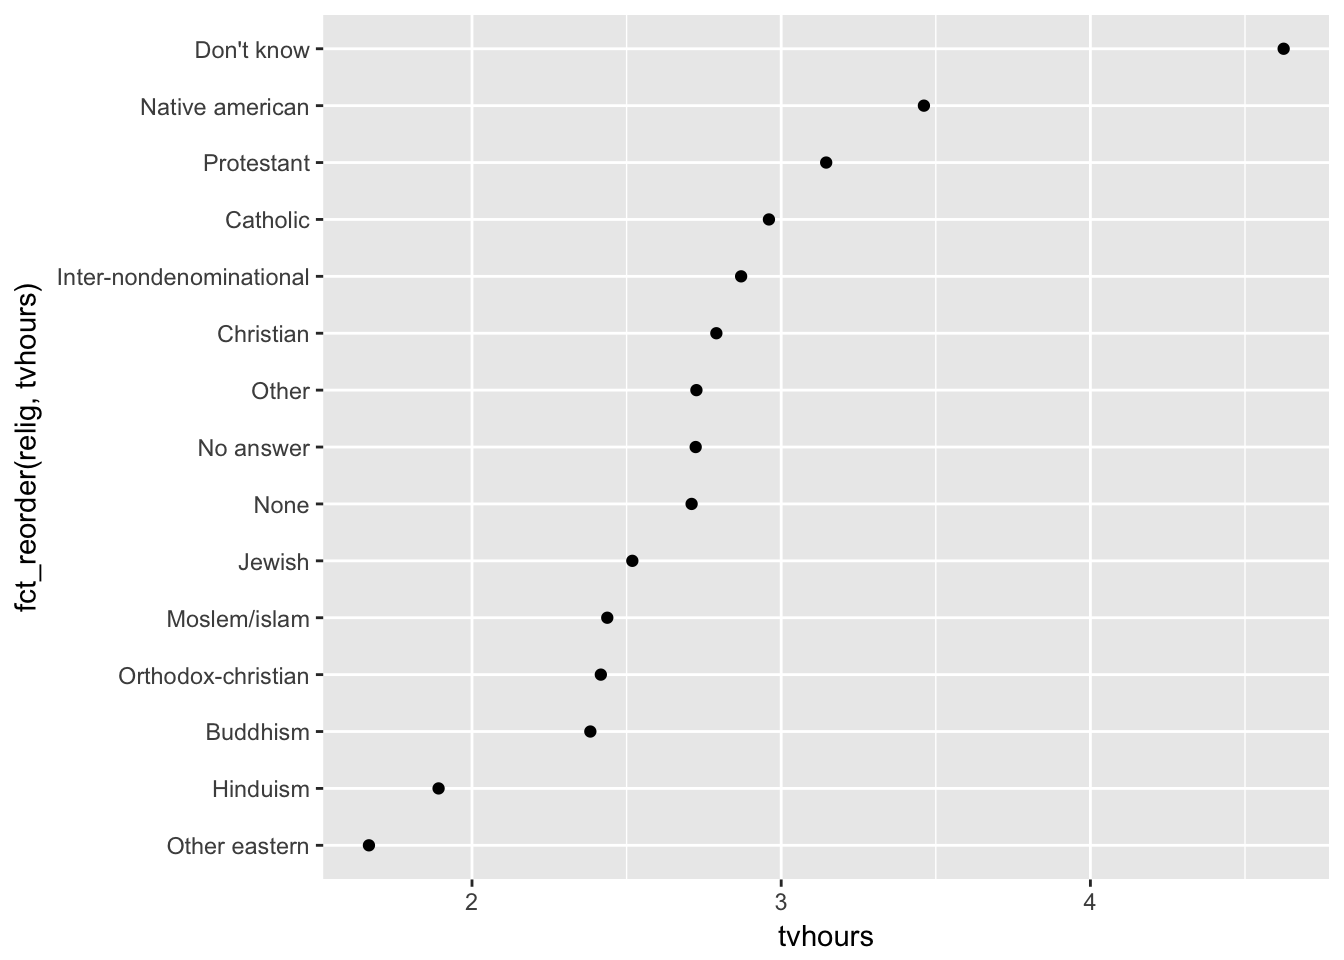
\includegraphics{main_files/figure-latex/unnamed-chunk-117-1.pdf}

\subsection{\texorpdfstring{\texttt{fct\_relevel()} tõstab joonisel osad
tasemed teistest
ettepoole}{fct\_relevel() tõstab joonisel osad tasemed teistest ettepoole}}\label{fct_relevel-tostab-joonisel-osad-tasemed-teistest-ettepoole}

Argumendid on faktor f ja need tasemed (jutumärkides), mida sa tahad
tõsta.

\begin{Shaded}
\begin{Highlighting}[]
\NormalTok{## täiendame eelmist graafikut ümberkorraldatud andmetega}
\NormalTok{p }\OperatorTok{+}\StringTok{ }\KeywordTok{aes}\NormalTok{(tvhours, }\KeywordTok{fct_relevel}\NormalTok{(relig, }\StringTok{"None"}\NormalTok{, }\StringTok{"Don't know"}\NormalTok{))}
\end{Highlighting}
\end{Shaded}

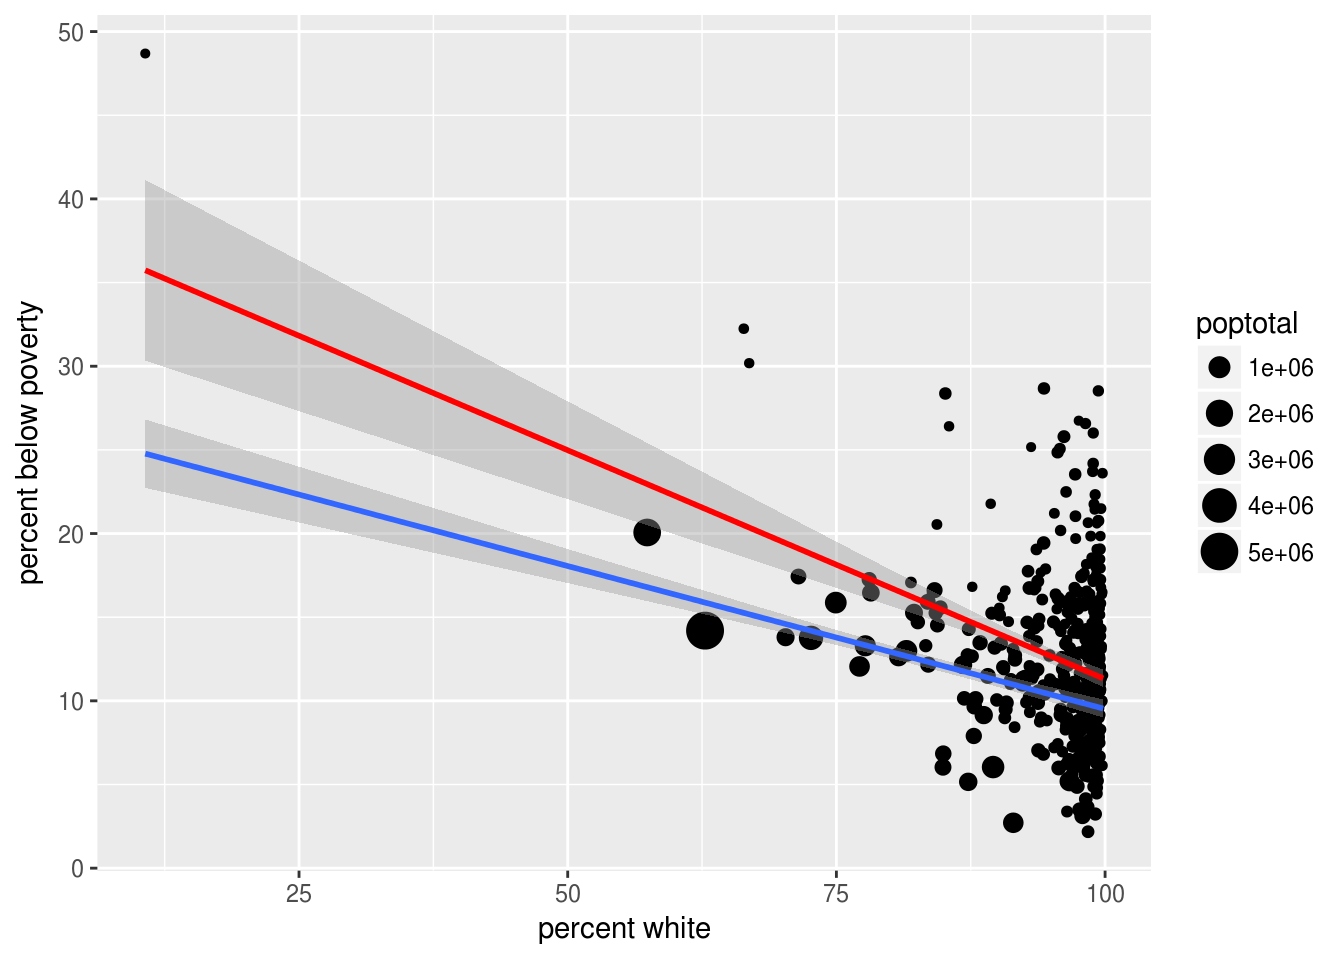
\includegraphics{main_files/figure-latex/unnamed-chunk-118-1.pdf}

\subsection{\texorpdfstring{Joontega plotil saab
\texttt{fct\_reorder2()} abil assotseerida y väärtused suurimate x
väärtustega}{Joontega plotil saab fct\_reorder2() abil assotseerida y väärtused suurimate x väärtustega}}\label{joontega-plotil-saab-fct_reorder2-abil-assotseerida-y-vaartused-suurimate-x-vaartustega}

See muudab ploti paremini jälgitavaks:

\begin{Shaded}
\begin{Highlighting}[]
\NormalTok{## summeerime andmed}
\NormalTok{gsscat_sum <-}\StringTok{ }\KeywordTok{filter}\NormalTok{(gss_cat, }\OperatorTok{!}\KeywordTok{is.na}\NormalTok{(age)) }\OperatorTok
\StringTok{  }\KeywordTok{group_by}\NormalTok{(age, marital) }\OperatorTok
\StringTok{  }\KeywordTok{mutate}\NormalTok{(}\DataTypeTok{N=}\KeywordTok{n}\NormalTok{())}
\NormalTok{## paneme andmed graafikule}
\KeywordTok{ggplot}\NormalTok{(gsscat_sum, }\KeywordTok{aes}\NormalTok{(age, N, }\DataTypeTok{colour =} \KeywordTok{fct_reorder2}\NormalTok{(marital, age, N))) }\OperatorTok{+}
\StringTok{  }\KeywordTok{geom_line}\NormalTok{() }\OperatorTok{+}
\StringTok{  }\KeywordTok{labs}\NormalTok{(}\DataTypeTok{colour =} \StringTok{"marital"}\NormalTok{)}
\end{Highlighting}
\end{Shaded}

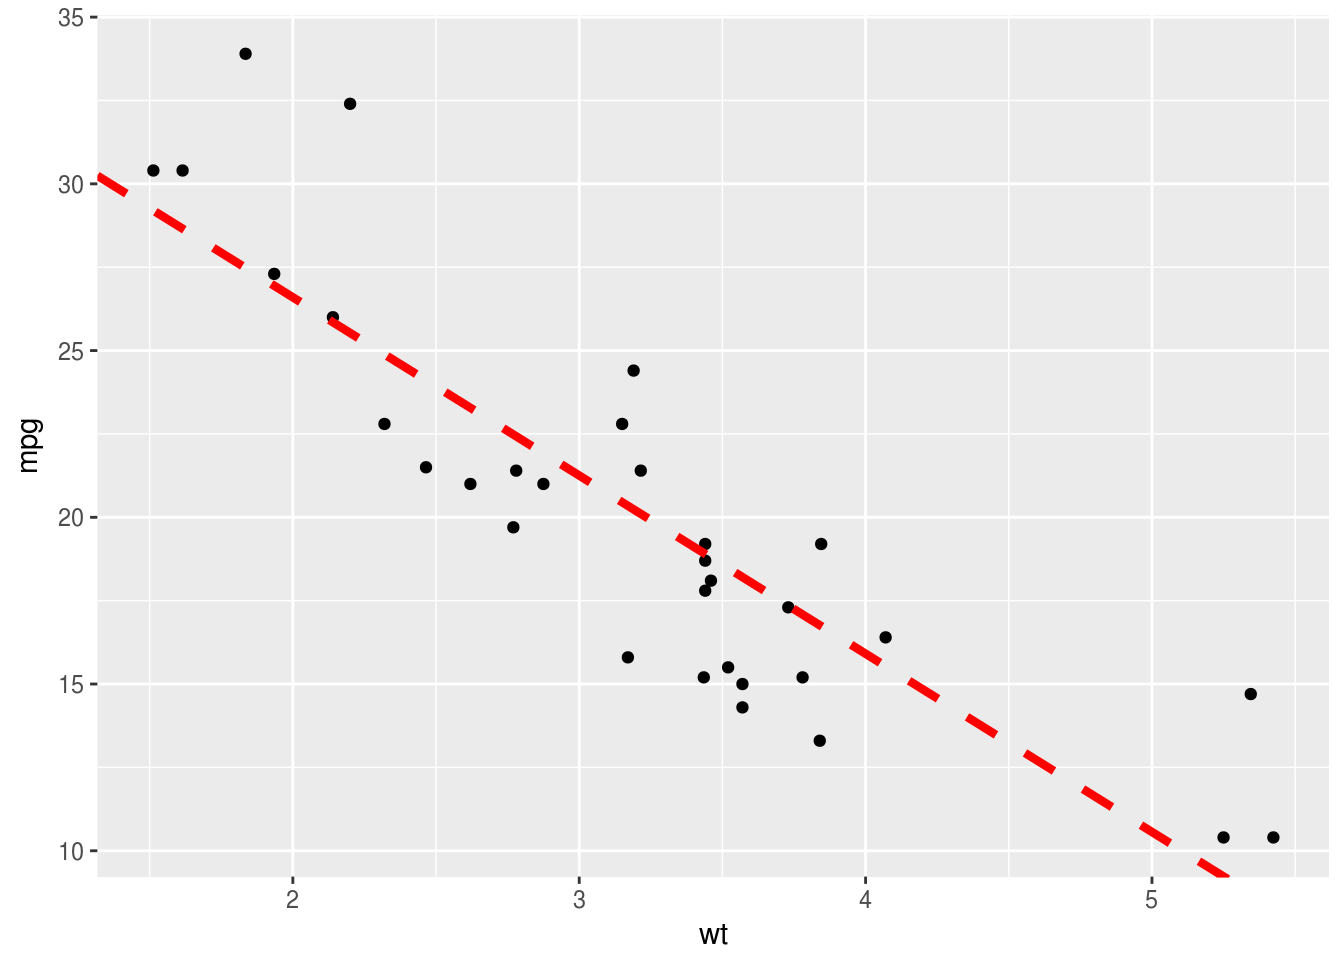
\includegraphics{main_files/figure-latex/unnamed-chunk-119-1.pdf}

\subsection{\texorpdfstring{Tulpdiagrammide korral kasuta
\texttt{fct\_infreq()}}{Tulpdiagrammide korral kasuta fct\_infreq()}}\label{tulpdiagrammide-korral-kasuta-fct_infreq}

Loeme kokku erineva perekondliku staatusega isikud ja paneme need andmed
tulpdiagrammi grupi suurusele vastupidises järjekorras st. väiksemad
grupid tulevad enne.

\begin{Shaded}
\begin{Highlighting}[]
\KeywordTok{mutate}\NormalTok{(gss_cat, }\DataTypeTok{marital =} \KeywordTok{fct_infreq}\NormalTok{(marital) }\OperatorTok\StringTok{ }\KeywordTok{fct_rev}\NormalTok{()) }\OperatorTok
\StringTok{  }\KeywordTok{ggplot}\NormalTok{(}\KeywordTok{aes}\NormalTok{(marital)) }\OperatorTok{+}\StringTok{ }\KeywordTok{geom_bar}\NormalTok{()}
\end{Highlighting}
\end{Shaded}

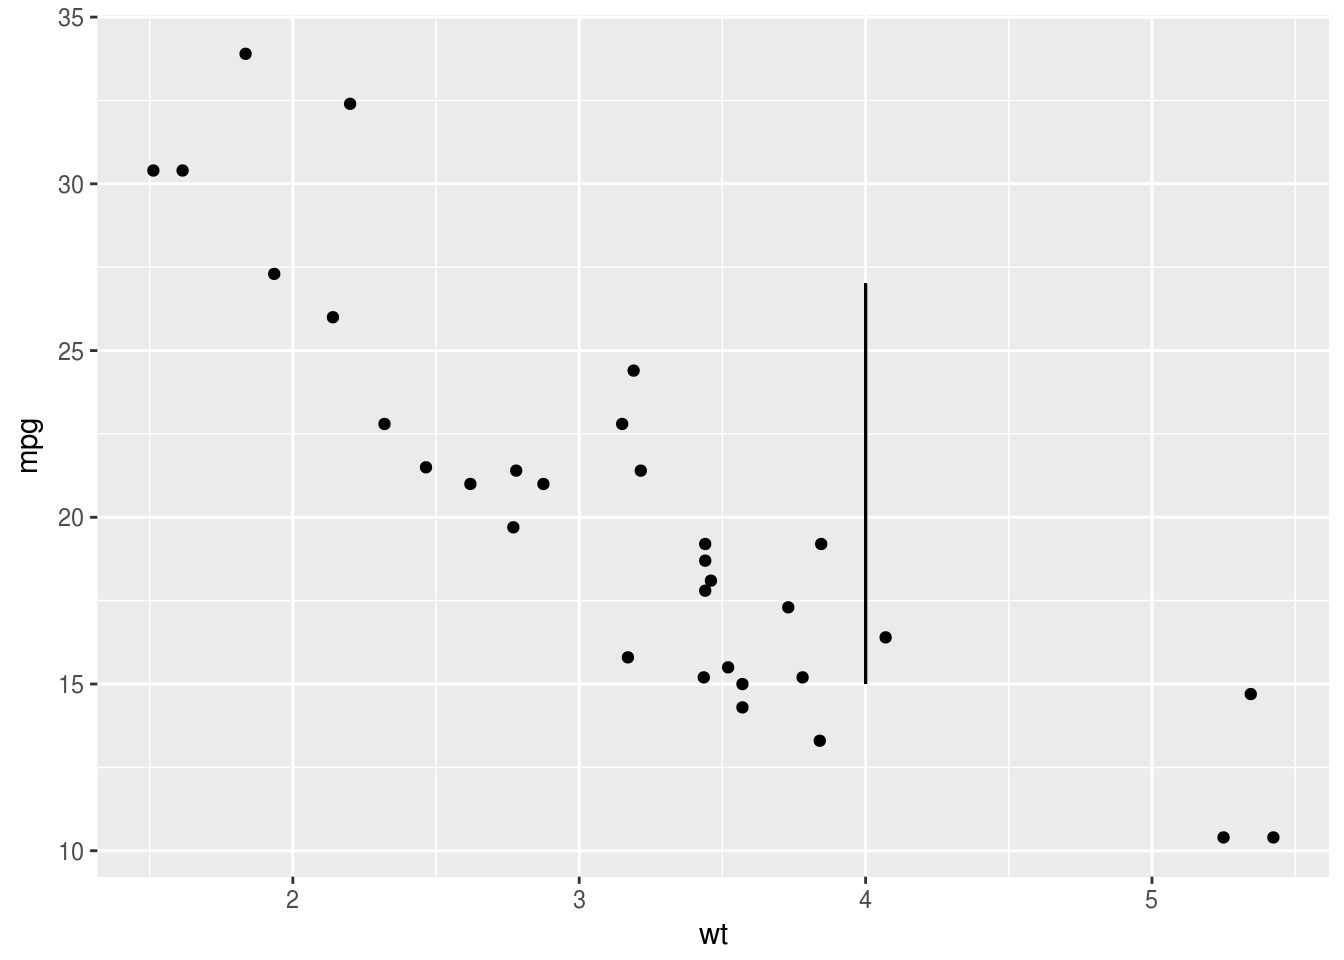
\includegraphics{main_files/figure-latex/unnamed-chunk-120-1.pdf}

\chapter{R on andmeanalüüsi keel, mille verbid on
funktsioonid}\label{funs}

Kasutaja ütleb nii täpselt kui oskab, mida ta tahab ja R-s elab kratt,
kes püüab ära arvata, mida on vaja teha. Vahest teeb kah. Vahest isegi
seda, mida kasutaja tahtis. Mõni arvab, et R-i puudus on veateadete
puudumine või krüptilised veateated. Sama kehtib ka R-i helpi kohta.
Seega tasub alati kontrollida, kas R ikka tegi seda, mida sina talle
enda arust ette kirjutasid.

Paljudel juhtudel ütleb (hea) funktsiooni nimi mida see teeb:

\begin{Shaded}
\begin{Highlighting}[]
\CommentTok{# create two test vectors}
\NormalTok{x <-}\StringTok{ }\KeywordTok{c}\NormalTok{(}\DecValTok{6}\NormalTok{, }\DecValTok{3}\NormalTok{, }\DecValTok{3}\NormalTok{, }\DecValTok{4}\NormalTok{, }\DecValTok{5}\NormalTok{)}
\NormalTok{y <-}\StringTok{ }\KeywordTok{c}\NormalTok{(}\DecValTok{1}\NormalTok{, }\DecValTok{3}\NormalTok{, }\DecValTok{4}\NormalTok{, }\DecValTok{2}\NormalTok{, }\DecValTok{7}\NormalTok{)}
\end{Highlighting}
\end{Shaded}

\begin{Shaded}
\begin{Highlighting}[]
\CommentTok{# calculate correlation}
\KeywordTok{cor}\NormalTok{(x, y)}
\end{Highlighting}
\end{Shaded}

\begin{verbatim}
## [1] -0.1166019
\end{verbatim}

\begin{Shaded}
\begin{Highlighting}[]
\CommentTok{# calculate sum}
\KeywordTok{sum}\NormalTok{(x)}
\end{Highlighting}
\end{Shaded}

\begin{verbatim}
## [1] 21
\end{verbatim}

\begin{Shaded}
\begin{Highlighting}[]
\CommentTok{# calculate sum of two vectors}
\KeywordTok{sum}\NormalTok{(x, y)}
\end{Highlighting}
\end{Shaded}

\begin{verbatim}
## [1] 38
\end{verbatim}

\begin{Shaded}
\begin{Highlighting}[]
\CommentTok{# calculate average}
\KeywordTok{mean}\NormalTok{(x)}
\end{Highlighting}
\end{Shaded}

\begin{verbatim}
## [1] 4.2
\end{verbatim}

\begin{Shaded}
\begin{Highlighting}[]
\CommentTok{# calculate median}
\KeywordTok{median}\NormalTok{(x)}
\end{Highlighting}
\end{Shaded}

\begin{verbatim}
## [1] 4
\end{verbatim}

\begin{Shaded}
\begin{Highlighting}[]
\CommentTok{# calculate standard deviation}
\KeywordTok{sd}\NormalTok{(x)}
\end{Highlighting}
\end{Shaded}

\begin{verbatim}
## [1] 1.30384
\end{verbatim}

\begin{Shaded}
\begin{Highlighting}[]
\CommentTok{# return quantiles}
\KeywordTok{quantile}\NormalTok{(x)}
\end{Highlighting}
\end{Shaded}

\begin{verbatim}
##   0%  25%  50%  75% 100% 
##    3    3    4    5    6
\end{verbatim}

\begin{Shaded}
\begin{Highlighting}[]
\CommentTok{# return maximum value}
\KeywordTok{max}\NormalTok{(x)}
\end{Highlighting}
\end{Shaded}

\begin{verbatim}
## [1] 6
\end{verbatim}

\begin{Shaded}
\begin{Highlighting}[]
\CommentTok{# return minimum value}
\KeywordTok{min}\NormalTok{(x)}
\end{Highlighting}
\end{Shaded}

\begin{verbatim}
## [1] 3
\end{verbatim}

R-is teevad asju programmikesed, mida kutsutakse
\textbf{funktsioonideks}. Te võite mõelda funktsioonist nagu verbist.
Näiteks funktsiooni \texttt{sum()} korral loe: ``võta summa''. Iga
funktsiooni nime järel on sulud. Nende sulgude sees asuvad selle
funktsiooni \textbf{argumendid}. Argumendid määravad ära funktsiooni
käitumise. Et näha, millised argumendid on funktsiooni käivitamiseks
vajalikud ja milliseid on üldse võimalik seadistada, kasuta `help'
käsku.

\begin{Shaded}
\begin{Highlighting}[]
\NormalTok{?sum}
\end{Highlighting}
\end{Shaded}

\begin{verbatim}
## Help on topic 'sum' was found in the following packages:
## 
##   Package               Library
##   mosaic                /Library/Frameworks/R.framework/Versions/3.4/Resources/library
##   base                  /Library/Frameworks/R.framework/Resources/library
##   Brobdingnag           /Library/Frameworks/R.framework/Versions/3.4/Resources/library
## 
## 
## Using the first match ...
\end{verbatim}

Help paneelis paremal all ilmub nüüd selle funktsiooni R
dokumentatsioon. Vaata seal peatükki Usage:
\texttt{sum(...,\ na.rm\ =\ FALSE)} ja edasi peatükki Arguments, mis
ütleb, et \texttt{...} (ellipsis) tähistab vektoreid.

\begin{verbatim}
sum {base}  R Documentation 
Sum of Vector Elements

Description:

sum returns the sum of all the values present in its arguments.

Usage

sum(..., na.rm = FALSE)

Arguments

... - numeric or complex or logical vectors.

na.rm   - logical. Should missing values (including NaN) be removed?
\end{verbatim}

Seega võtab funktsioon \texttt{sum()} kaks argumenti: vektori arvudest
(või loogilise vektori, mis koosneb TRUE ja FALSE määrangutest), ning
``na.rm'' argumendi, millele saab anda väärtuseks kas, TRUE või FALSE.
Usage ütleb ka, et vaikimisi on \texttt{na.rm\ =\ FALSE}, mis tähendab,
et sellele argumendile on antud vaikeväärtus -- kui me seda ise ei
muuda, siis jäävad NA-d arvutusse sisse. Kuna NA tähendab ``tundmatu
arv'' siis iga tehe NA-dega annab vastuseks ``tundmatu arv'' ehk NA
(tundmatu arv + 2 = tundmatu arv). Seega NA tulemus annab märku, et teie
andmetes võib olla midagi valesti.

\begin{Shaded}
\begin{Highlighting}[]
\NormalTok{## moodustame vektori}
\NormalTok{apples <-}\StringTok{ }\KeywordTok{c}\NormalTok{(}\DecValTok{1}\NormalTok{, }\DecValTok{34}\NormalTok{, }\DecValTok{43}\NormalTok{, }\OtherTok{NA}\NormalTok{)}
\NormalTok{## arvutame summa}
\KeywordTok{sum}\NormalTok{(apples, }\DataTypeTok{na.rm =} \OtherTok{TRUE}\NormalTok{)}
\end{Highlighting}
\end{Shaded}

\begin{verbatim}
## [1] 78
\end{verbatim}

Niimoodi saab arvutada summat vektorile nimega ``apples''.

Sisestades R käsureale funktsiooni ilma selle sulgudeta saab masinast
selle funktsiooni koodi. Näiteks:

\begin{Shaded}
\begin{Highlighting}[]
\NormalTok{sum}
\end{Highlighting}
\end{Shaded}

\begin{verbatim}
## function (x, ..., data = NULL, groups = NULL, na.rm = getOption("na.rm", 
##     FALSE)) 
## {
##     if (lazyeval::is_formula(x)) {
##         if (is.null(data)) 
##             data <- lazyeval::f_env(x)
##         formula <- mosaicCore::mosaic_formula_q(x, groups = groups, 
##             max.slots = 3)
##         return(maggregate(formula, data = data, FUN = base::sum, 
##             ..., na.rm = na.rm, .multiple = FALSE))
##     }
##     base::sum(x, ..., na.rm = na.rm)
## }
## <environment: namespace:mosaic>
\end{verbatim}

Tulemus näitab, et \texttt{sum()} on \texttt{Primitive} funktsioon, mis
põhimõtteliselt tähendab, et ta põhineb C koodil ja ei kasuta R koodi.

\section{Kirjutame oma esimese R
funktsiooni}\label{kirjutame-oma-esimese-r-funktsiooni}

Võib ju väita, et funktsiooni ainus mõte on peita teie eest korduvad
vajalikud koodiread kood funktsiooni nime taha. Põhjus, miks R-s on
funktsioonid, on korduse vähendamine, koodi loetavaks muutmine ja seega
ka ruumi kokkuhoid. Koodi funktsioonidena kasutamine suurendab
analüüside reprodutseeritavust, kuna funktsioonis olev kood pärineb
ühest allikast, mitte ei ole paljude koopiatena igal pool laiali. See
muudab pikad koodilõigud hõlpsalt taaskasutatavaks sest lihtsam on
kirjutada lühike funktsiooni nimi ja sisestada selle funktsiooni
argumendid. Koodi funktsioonidesse kokku surumine vähendab võimalusi
lollideks vigadeks, mida te võite teha pikkade koodijuppidega
manipuleerides. Seega tasub teil õppida ka oma korduvaid koodiridu
funktsioonidena vormistama.

Kõige pealt kirjutame natuke koodi.

\begin{Shaded}
\begin{Highlighting}[]
\CommentTok{# two apples}
\NormalTok{apples <-}\StringTok{ }\DecValTok{2}
\CommentTok{# three oranges}
\NormalTok{oranges <-}\StringTok{ }\DecValTok{3} 
\CommentTok{# parentheses around expression assigning result to an object }
\CommentTok{# ensure that result is also printed to R console}
\NormalTok{(inventory <-}\StringTok{ }\NormalTok{apples }\OperatorTok{+}\StringTok{ }\NormalTok{oranges)}
\end{Highlighting}
\end{Shaded}

\begin{verbatim}
## [1] 5
\end{verbatim}

Ja nüüd pakendame selle tehte funktsiooni \texttt{add2()}. Funktsiooni
defineerimiseks kasutame järgmist r ekspressiooni
\texttt{function(\ arglist\ )\ expr}, kus ``arglist'' on tühi või ühe
või rohkema nimega argumenti kujul \texttt{name=expression}; ``expr'' on
R-i ekspressioon st. kood mida see funktsioon käivitab. Funktsiooni
viimane evlueeritav koodirida on see, mis tuleb välja selle funktsiooni
outputina.

All toodud näites on selleks \texttt{x\ +\ y} tehte vastus.

\begin{Shaded}
\begin{Highlighting}[]
\NormalTok{add2 <-}\StringTok{ }\ControlFlowTok{function}\NormalTok{(x, y) \{}
\NormalTok{    x }\OperatorTok{+}\StringTok{ }\NormalTok{y}
\NormalTok{\}}
\end{Highlighting}
\end{Shaded}

Seda koodi jooksutades näeme, et meie funktsioon ilmub R-i Environmenti,
kuhu tekib Functions lahter. Seal on näha ka selle funktsiooni kaks
argumenti, apples ja oranges.

Antud funktsiooni käivitamine annab veateate, sest funktsiooni
argumentidel pole väärtusi:

\begin{Shaded}
\begin{Highlighting}[]
\NormalTok{## run function in failsafe mode}
\NormalTok{inventory <-}\StringTok{ }\KeywordTok{try}\NormalTok{(}\KeywordTok{add2}\NormalTok{())}
\NormalTok{## when function fails, error message is returned}
\KeywordTok{class}\NormalTok{(inventory)}
\end{Highlighting}
\end{Shaded}

\begin{verbatim}
## [1] "try-error"
\end{verbatim}

\begin{Shaded}
\begin{Highlighting}[]
\NormalTok{## print error message}
\KeywordTok{cat}\NormalTok{(inventory)}
\end{Highlighting}
\end{Shaded}

\begin{verbatim}
## Error in add2() : argument "x" is missing, with no default
\end{verbatim}

Andes funktsiooni argumentidele väärtused, saab väljundi:

\begin{Shaded}
\begin{Highlighting}[]
\NormalTok{## run function with proper arguments}
\NormalTok{inventory <-}\StringTok{ }\KeywordTok{add2}\NormalTok{(}\DataTypeTok{x =}\NormalTok{ apples, }\DataTypeTok{y =}\NormalTok{ oranges)}
\NormalTok{## numeric vector is returned}
\KeywordTok{class}\NormalTok{(inventory)}
\end{Highlighting}
\end{Shaded}

\begin{verbatim}
## [1] "numeric"
\end{verbatim}

\begin{Shaded}
\begin{Highlighting}[]
\NormalTok{## result}
\NormalTok{inventory}
\end{Highlighting}
\end{Shaded}

\begin{verbatim}
## [1] 5
\end{verbatim}

\textbf{Nüüd midagi kasulikumat.}

Funktsioon standrardvea arvutamiseks (baas R-s sellist funktsiooni ei
ole): \texttt{sd()} funktsioon arvutab standardhälbe. Sellel on kaks
argumenti: x and \ldots{} and data and groups and na.rm. Me teame, et
SEM=SD/sqrt(N) kus N = length(x)

\begin{Shaded}
\begin{Highlighting}[]
\NormalTok{calc_sem <-}\StringTok{ }\ControlFlowTok{function}\NormalTok{(x) \{}
\NormalTok{  stdev <-}\StringTok{ }\KeywordTok{sd}\NormalTok{(x)}
\NormalTok{  n <-}\StringTok{ }\KeywordTok{length}\NormalTok{(x)}
\NormalTok{  stdev }\OperatorTok{/}\StringTok{ }\KeywordTok{sqrt}\NormalTok{(n)}
\NormalTok{\}}
\end{Highlighting}
\end{Shaded}

x hoiab lihtsalt kohta andmetele, mida me tahame sinna funktsiooni
suunata. \texttt{sd()}, \texttt{sqrt()} ja \texttt{length()} on
olemasolevad baas R funktsioonid, mille me oma funktsiooni hõlmame.

\begin{Shaded}
\begin{Highlighting}[]
\NormalTok{## create numeric vector}
\NormalTok{numbers <-}\StringTok{ }\KeywordTok{c}\NormalTok{(}\DecValTok{2}\NormalTok{, }\FloatTok{3.4}\NormalTok{, }\DecValTok{54}\NormalTok{, }\OtherTok{NA}\NormalTok{, }\DecValTok{3}\NormalTok{)}
\KeywordTok{calc_sem}\NormalTok{(numbers)}
\end{Highlighting}
\end{Shaded}

\begin{verbatim}
## [1] NA
\end{verbatim}

No jah, kui meil on andmetes tundmatu arv (\texttt{NA}) siis on ka
tulemuseks tundmatu arv.

Sellisel juhul tuleb NA väärtused vektorist enne selle funktsiooni
kasutamist välja visata:

\begin{Shaded}
\begin{Highlighting}[]
\NormalTok{numbers_filtered <-}\StringTok{ }\KeywordTok{na.omit}\NormalTok{(numbers)}
\KeywordTok{calc_sem}\NormalTok{(numbers_filtered)}
\end{Highlighting}
\end{Shaded}

\begin{verbatim}
## [1] 12.80338
\end{verbatim}

On ka võimalus funktsiooni sisse kirjutada \textbf{NA väärtuste
käsitlemine}. Näiteks, üks võimalus on \textbf{anda viga} ja funktsioon
katkestada, et kasutaja saaks ise ühemõtteliselt oma andmetest NA
väärtused eemaldada. Teine võimalus on funktsioonis \textbf{NA-d
vaikimisi eemaldada} ja anda selle kohta näiteks teade.

NA-de vaikimisi eemaldamiseks on hetkel mitu võimalust, kasutame
kõigepealt nö. valet lahendust:

\begin{Shaded}
\begin{Highlighting}[]
\NormalTok{calc_sem <-}\StringTok{ }\ControlFlowTok{function}\NormalTok{(x) \{}
\NormalTok{  ## kasutame sd funktsiooni argumenti na.rm}
\NormalTok{  stdev <-}\StringTok{ }\KeywordTok{sd}\NormalTok{(x, }\DataTypeTok{na.rm =} \OtherTok{TRUE}\NormalTok{)}
\NormalTok{  n <-}\StringTok{ }\KeywordTok{length}\NormalTok{(x)}
\NormalTok{  stdev }\OperatorTok{/}\StringTok{ }\KeywordTok{sqrt}\NormalTok{(n)}
\NormalTok{\}}

\KeywordTok{calc_sem}\NormalTok{(numbers)}
\end{Highlighting}
\end{Shaded}

\begin{verbatim}
## [1] 11.4517
\end{verbatim}

See annab meile vale tulemuse sest \texttt{na.rm\ =\ TRUE} viskab küll
NA-d välja meie vektorist aga jätab vektori pikkuse muutmata
(\texttt{length(x)} rida).

Teeme uue versiooni oma funktsioonist, mis viskab vaikimisi välja
puuduvad väärtused, kui need on olemas ja annab siis ka selle kohta
hoiatuse.

\begin{Shaded}
\begin{Highlighting}[]
\NormalTok{## x on numbriline vektor}
\NormalTok{calc_sem <-}\StringTok{ }\ControlFlowTok{function}\NormalTok{(x) \{}
  
\NormalTok{  ## viskame NA väärtused vektorist välja}
\NormalTok{  x <-}\StringTok{ }\KeywordTok{na.omit}\NormalTok{(x)}
  
\NormalTok{  ## kui vektoris on NA väärtusi, siis hoiatame kasutajat}
  \ControlFlowTok{if}\NormalTok{(}\KeywordTok{inherits}\NormalTok{(}\KeywordTok{na.action}\NormalTok{(x), }\StringTok{"omit"}\NormalTok{)) \{}
    \KeywordTok{warning}\NormalTok{(}\StringTok{"Removed NAs from vector.}\CharTok{\textbackslash{}n}\StringTok{"}\NormalTok{)}
\NormalTok{  \}}
  
\NormalTok{  ## arvutame standardvea kasutades filtreeritud vektorit}
\NormalTok{  stdev <-}\StringTok{ }\KeywordTok{sd}\NormalTok{(x)}
\NormalTok{  n <-}\StringTok{ }\KeywordTok{length}\NormalTok{(x)}
\NormalTok{  stdev }\OperatorTok{/}\StringTok{ }\KeywordTok{sqrt}\NormalTok{(n)}
\NormalTok{\}}

\KeywordTok{calc_sem}\NormalTok{(numbers)}
\end{Highlighting}
\end{Shaded}

\begin{verbatim}
## Warning in calc_sem(numbers): Removed NAs from vector.
\end{verbatim}

\begin{verbatim}
## [1] 12.80338
\end{verbatim}

\begin{Shaded}
\begin{Highlighting}[]
\KeywordTok{length}\NormalTok{(numbers)}
\end{Highlighting}
\end{Shaded}

\begin{verbatim}
## [1] 5
\end{verbatim}

Missugune funktsiooni käitumine valida, sõltub kasutaja vajadusest.
Rohkem infot NA käsitlemise funktsioonide kohta saab \texttt{?na.omit}
abifailist.

Olgu see õpetuseks, et funktsioonide kirjutamine on järk-järguline
protsess ja sellele, et alati saab paremini teha.

\section{Funktsioonide raamatukogud}\label{funktsioonide-raamatukogud}

Kõige esimene sõnum \texttt{sum()} help lehel on ``sum \{base\}'', mis
tähendab, et see funktsioon kuulub nn. baasfunktsioonide hulka. Need
funktsioonid on alati kättesaadavad sest neid sisaldavad raamatukogud
laetakse vaikimisi teie töökeskkonda. Näiteks ``base'' raamatukogu
versioon 3.4.1 sisaldab 453 funktsiooni. Enamasti on sarnaseid asju
tegevad funktsioonid koondatud kokku raamatukogudesse ehk pakettidesse,
mis tuleb eraldi R kesksest repositooriumist
\href{https://cran.r-project.org}{CRAN} alla laadida ja installeerida.

Selleks, et kasutada raamatukogudes leiduvaid funktsioone, tuleb
kõigepealt antud raamatukogu oma arvutisse alla laadida (seda peab
tegema ainult üks kord) ja seejärel see raamatukogu töökeskkond sisse
lugeda (seda tuleb teha igal R sessioonil, kus me vastava raamatukogu
funktsioone kasutame).

Näiteks, hea laps ei lahku kunagi kodust ilma raamatukogu
``tidyverse''-ta.

Kõigepealt installeerime selle oma arvutisse.

\begin{Shaded}
\begin{Highlighting}[]
\KeywordTok{install.packages}\NormalTok{(}\StringTok{"tidyverse"}\NormalTok{)}
\end{Highlighting}
\end{Shaded}

NB! kui mõni raamatukogu sel viisil alla ei tule, siis guugeldage selle
nime + R ja vaadake instruktsioone allalaadimiseks.

Raamatukogud elavad \emph{repositorides}, millest suurim on CRAN.
\texttt{install.packages()} otsib, laadib alla ja installeerib teie
soovitud raamatukogu just sealt. Teised suuremad repod on GitHub
\url{https://github.com}, kus elab sageli R pakettide source kood ja dev
versioonid, ja Bioconductor (seal on tuhandeid bioloogiliseks analüüsiks
vajalikke pakette). Neist allalaadimine on pisut erinev, aga mitte kuigi
keeruline. Kõigi pakettide kohta on võrgus ka allalaadimise õpetus.
Googeldage paketi nime järgi.

Nüüd on teil \texttt{tidyverse} pakett arvutis. Tegelikult kuuluvad siia
raamatukokku omakorda tosinkond raamatukogu --- tidyverse on pisut meta.
Igal juhul muutuvad selle funktsioonid kättesaadavaks peale seda, kui te
need töökeskkonda sisse loete

Veel üks tehniline detail. \texttt{library(tidyverse)} käsk ei loe sisse
kõiki alam-raamatukogusid, mis selle nime all CRAN-ist alla laaditi.
Need tuleb vajadusel eraldi ükshaaval sisse lugeda.

\begin{Shaded}
\begin{Highlighting}[]
\KeywordTok{library}\NormalTok{(tidyverse)}
\end{Highlighting}
\end{Shaded}

Antud kursuse raames tuleb seda teha iga kord, kui te R sessiooni
alustate. Pakette/library-sid on soovitav laadida töökeskkonda muidu
ikka ainult vastavalt vajadusele. ``tidyverse''-gi puhul on soovitatav
eelistatult laadida ainult see/need raamatukogud, mida tegelikult
kasutama ka hakatakse. Vaikimisi kogu aeg kogu ``tiduverse'' rammatukogu
laadimine ei pruugi olla reprodutseeritavuse mõttes hea, sest
paratamatult võivad tekkida konfliktid teiste mitte-tidyverse
raamatukogude funktsioonidega. Näiteks on \texttt{select()} funktsioon
lisaks ``dplyr'' librarile olemas ka mitmes teises paketis.

Konfliktide korral eri pakettide sama nimega funktsioonide vahel saab
\texttt{::} operaatorit kasutades kutsuda välja/importida funktsiooni
spetsiifilisest paketist:

\begin{Shaded}
\begin{Highlighting}[]
\NormalTok{tidyr}\OperatorTok{::}\KeywordTok{select}\NormalTok{(df, my_var)}
\end{Highlighting}
\end{Shaded}

Sellisel kujul funktsioonide kasutamisel pole vaja imporditavat
funktsiooni sisaldavat raamatukogu töökeskkonda laadida.

\section{Paiguta kõigi raamatukogude lugemine koodi
algusesse}\label{paiguta-koigi-raamatukogude-lugemine-koodi-algusesse}

Enamasti kirjutatakse sisse loetavad raamatukogud kohe R scripti
algusesse. Siis on teile endale ja teistele kes teie koodi loevad ilusti
näha, mida hiljem vaja läheb.

Kui te lähete RStudios paremal all olevale ``Packages'' tabile, siis on
võimalik klikkida raamatukogu nimele ja näha selle help-faile,
tutooriale ja kõiki selle raamatukogu funktsioone koos nende help
failidega.

Nüüd võite näiteks kasutada funktsiooni \texttt{drop\_na()}, mis
eemaldab teie andmetabelist read, mis sisaldavad NA-sid. See funktsioon
asub ``tidyr'' raamatukogus, mis koos ülejäänud ``tidyverse''-ga sisse
loeti.

\begin{Shaded}
\begin{Highlighting}[]
\NormalTok{?drop_na}
\end{Highlighting}
\end{Shaded}

Verb: \texttt{drop\_na()} loe: ``viska NA-d välja''.

\begin{Shaded}
\begin{Highlighting}[]
\CommentTok{# creates a two-column table}
\NormalTok{df <-}\StringTok{ }\KeywordTok{tibble}\NormalTok{(}\DataTypeTok{apples =} \KeywordTok{c}\NormalTok{(}\DecValTok{2}\NormalTok{, }\DecValTok{3}\NormalTok{, }\OtherTok{NA}\NormalTok{, }\DecValTok{5}\NormalTok{), }\DataTypeTok{oranges =} \KeywordTok{c}\NormalTok{(}\DecValTok{4}\NormalTok{, }\OtherTok{NA}\NormalTok{, }\DecValTok{6}\NormalTok{, }\DecValTok{4}\NormalTok{)) }
\NormalTok{df}
\end{Highlighting}
\end{Shaded}

\begin{verbatim}
## # A tibble: 4 x 2
##   apples oranges
##    <dbl>   <dbl>
## 1      2       4
## 2      3      NA
## 3     NA       6
## 4      5       4
\end{verbatim}

Nüüd filtreerime tabelist välja selle rea mis sisaldavad NA väärtusi
tulbas ``apples''. Tabeli mõlemas tulbas on üks NA, seega jääb tabelisse
tulbas ``oranges'' NA-d sisaldav rida alles.

\begin{Shaded}
\begin{Highlighting}[]
\NormalTok{df1 <-}\StringTok{ }\KeywordTok{drop_na}\NormalTok{(df, apples) }
\NormalTok{df1}
\end{Highlighting}
\end{Shaded}

\begin{verbatim}
## # A tibble: 3 x 2
##   apples oranges
##    <dbl>   <dbl>
## 1      2       4
## 2      3      NA
## 3      5       4
\end{verbatim}

\section{Hurraa, uus arvuti! aga mis libraryd mul
olid\ldots{}}\label{hurraa-uus-arvuti-aga-mis-libraryd-mul-olid}

Kui te uuendate oma R versiooni või olete ostnud uue arvuti, siis
lähevad kaduma kõik teie paketid. Nende automaatseks allalaadimiseks
võite teha nii:

\begin{Shaded}
\begin{Highlighting}[]
\NormalTok{## in the old version/machine run:}
\NormalTok{installed <-}\StringTok{ }\KeywordTok{as.data.frame}\NormalTok{(}\KeywordTok{installed.packages}\NormalTok{())}
\KeywordTok{write.csv}\NormalTok{(installed, }\StringTok{"data/installed_previously.csv"}\NormalTok{)}

\NormalTok{## when new machine, move "data/installed_previously.csv" into new computer}

\NormalTok{## and in the new one:}
\NormalTok{installedPreviously <-}\StringTok{ }\KeywordTok{read.csv}\NormalTok{(}\StringTok{"data/installed_previously.csv"}\NormalTok{)}
\NormalTok{baseR <-}\StringTok{ }\KeywordTok{as.data.frame}\NormalTok{(}\KeywordTok{installed.packages}\NormalTok{())}
\NormalTok{toInstall <-}\StringTok{ }\KeywordTok{setdiff}\NormalTok{(installedPreviously}\OperatorTok{$}\NormalTok{Package, baseR}\OperatorTok{$}\NormalTok{Package)}
\KeywordTok{install.packages}\NormalTok{(toInstall) }
\end{Highlighting}
\end{Shaded}

Tundub juskui tark ja mõistlik, kuid:

\begin{itemize}
\tightlist
\item
  Massiline pakettide installatsioon uude arvutisse võib kergesti
  takerduda erinevate R-i väliste sõltuvuste taha ja tekitab
  frustratsiooni.
\item
  Lisaks, ebavajalikest pakettidest vabanemiseks on mõistlik vajaminevad
  paketid jooksvalt tagasi installeerida.
\item
  Kiire internet on laialt saadaval ja ka kompileeritavad paketid ei
  võta installatsiooniks rohkem kui mõni minut aega.
\end{itemize}

\chapter{Bayesiaanlik statistika}\label{bayesiaanlik-statistika}

\section{Ajaloost ja tõenäosusest}\label{ajaloost-ja-toenaosusest}

Bayesiaanlik ja sageduslik statistika leiutati üksteise järel
Pierre-Simon Laplace poolt, kes arendas välja kõigepealt bayesi
statistika alused ning seejärel sagedusliku statistika omad (ca. 1800 -
1812). Sagedusliku statistika tekkimise ja hilisema õitsengu põhjus 20.
sajandil oli arvutuslik lihtsus. Bayesi meetoditega ei olnud võimalik
korralikult teadust teha enne 1990-ndaid aastaid, mil personaalarvutite
levik algatas buumi nende meetodite arendamises. Praegu on maailmas
bayesi ja sageduslikku statistikat umbes pooleks (vähemalt uute
meetodite arendustöö poole pealt). Eestis bayesi statistika 2017 aasta
seisuga peaaegu, et puudub.

Kahe statistika põhiline erinevus ei tule matemaatikast --- mõlemad
harud lähtuvad samadest tõenäosusteooria aksioomidest ja nende vahel
puuduvad matemaatilised lahkarvamused --- vaid tõenäosuse tõlgendusest.

Bayesi tõlgenduses on tõenäosus teadlase usu määr mingi hüpoteesi
kehtimisse. Hüpotees võib näiteks olla, et järgmise juulikuu sademete
hulk Vilsandil jääb vahemikku 22 kuni 34 mm. Kui Bayesi arvutus annab
selle hüpoteesi tõenäosuseks 0.57, siis oleme me selle teadmise najal
nõus maksma mitte rohkem kui 57 senti kihlveo eest, mille alusel
makstakse juhul, kui see hüpotees tõeseks osutub, välja 1 EUR (ja me
saame vähemalt 43 senti kasumit).

Sageduslikud statistikud usuvad, et selline tõenäosuse tõlgendus on
ebateaduslik, kuna see on ``subjektiivne''. On võimalik, et n teadlast
arvutavad korrektselt samade andmete põhjal n erinevat tõenäosust ja
usuvad seega samade tõendite põhjal erinevaid asju. See võib juhtuda
siis, kui nad lähtuvad väga erinevatest taustauskumustest oma
hüpoteeside kehtimise kohta. Kui te usute, et teie taustateadmised ei
tohi mingil juhul mõjutada järeldusi, mis te oma andmete põhjal teete,
siis te ei ole bayesiaan. Sel juhul pakub alternatiivi sageduslik
tõenäosuse tõlgendus. Sageduslik tõenäosus on defineeritud kui teatud
tüüpi andmete esinemise pikaajaline suhteline sagedus. Näiteks, kui me
viskame münti palju kordi, siis peaks kullide (või kirjade) suhteline
sagedus meile andma selle mündi tõenäosuse langeda kiri üleval. Selline
tõenäosus on omistatav ainult sellistele sündmustele, mille esinemisel
on sagedus. Teaduslik teooria ei ole selline sündmus. Seega ei ole
sageduslikus statistikas võimalik rääkida ka hüpoteesi kehtimise
tõenäosusest. Sageduslik lahendus on selle asemel, et rääkida meie
hüpoteesi tõenäosusest meie andmete korral, rääkida andmete, mis
sarnanevad meie andmetega, esinemise tõenäosusest null-hüpoteesi (mis ei
ole meie hüpotees) kehtimise korral. Seega omistatakse sagedus (=
tõenäosus) andmetele, mitte hüpoteesile. Järgnevalt toome näite, kuidas
bayesiaan ja sageduslik statistik lahendavad sama ülesande.

\subsection{Näide: kahe grupi võrdlus}\label{naide-kahe-grupi-vordlus}

meil on 2 gruppi, katse ja kontroll, millest kummagis 30 mõõtmist ja me
soovime teada, kui palju katsetingimus mõjutab mõõtmistulemust. Meie
andmed on normaaljaotusega ja andmepunktid, mida me analüüsime, on
efektisuurused (katse1 - kontroll1 = es1 jne).

\subsubsection{Bayesiaan}\label{bayesiaan}

Statistiline küsimus on Bayesiaanil ja sageduslikul statistikul sama:
kas ja kui palju erinevad kahe grupi keskväärtused? Bayesiaan alustab
sellest, et ehitab kaks mudelit: andmete tõepäramudel ja taustateadmiste
mudel ehk prior.

Kui andmed on normaaljaotusega, siis on ka tõepäramudel normaaljaotus.
Alustame sellest, et fitime oma valimiandmed (üksikud efekti suurused)
normaaljaotuse mudelisse.

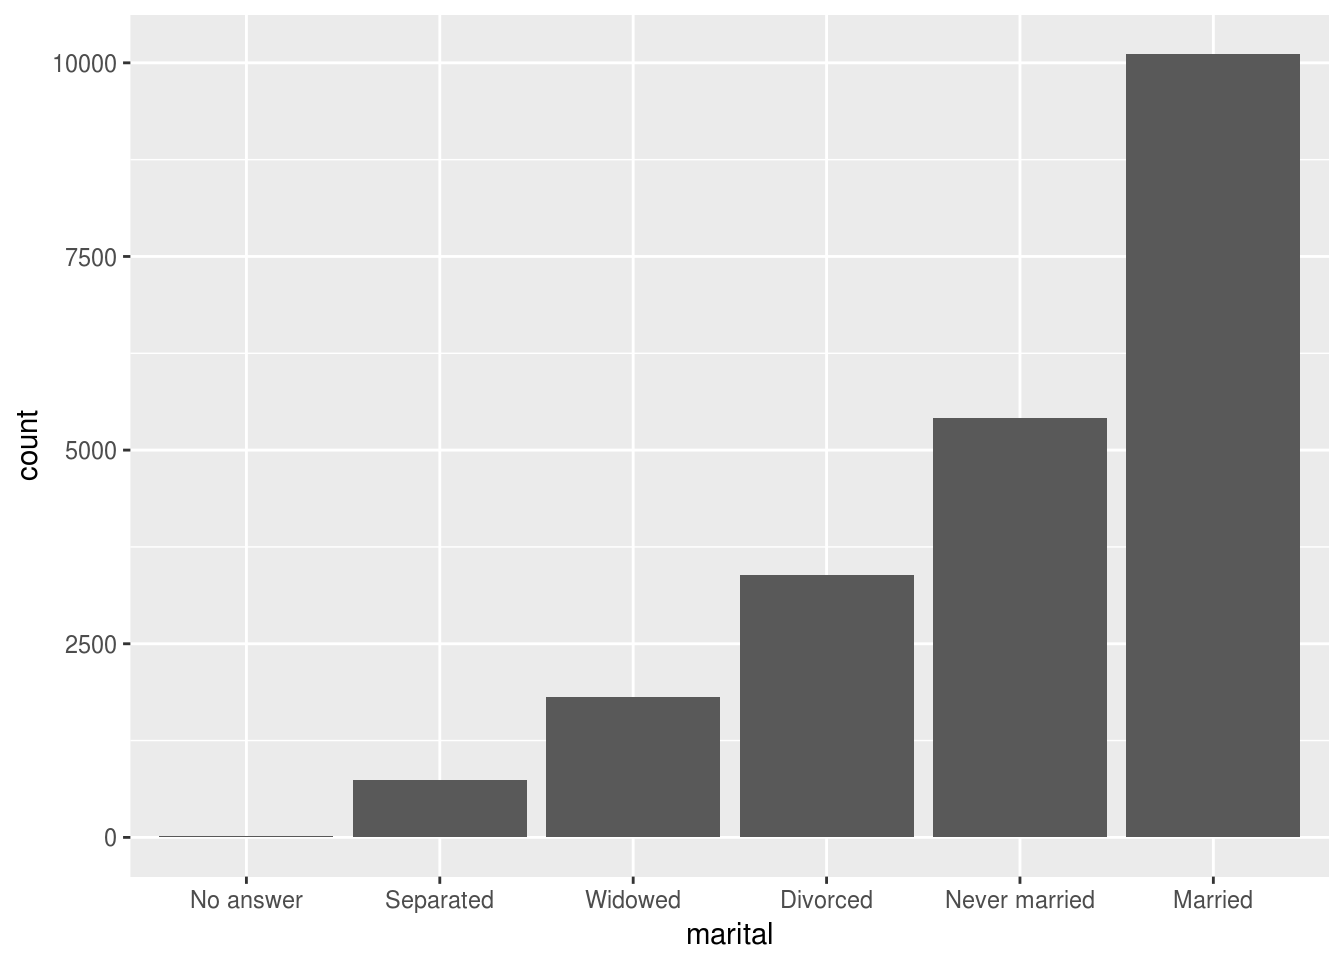
\includegraphics{main_files/figure-latex/unnamed-chunk-143-1.pdf}

\textbf{Joonis 1. paariviisiline katse - kontroll disain. Katset on
korratud 30 korda. X teljel on effekti suurused (ES). 30 ES-i on
näidatud punktidena. Must joon näitab keskmist ES-i. Andmed on
mudeldatud normaaljaotusena.}

See ei ole veel tõepäramudel, sest me tahame hinnangut ES
\textbf{keskväärtuse} kõige tõenäolisemale väärtusele, ja lisaks veel
hinnangut ebakindlusele selle punkt-hinnangu ümber (usalduslpiire).
Seega tuleb eelmine jaotus kitsamaks tõmmata, et ta kajastaks meie
teadmisi ES-ide keskväärtuste, mitte individuaalsete ES-de, kohta. Uue
jaotusmudeli sd = eelmise jaotuse sd/sqrt(30).

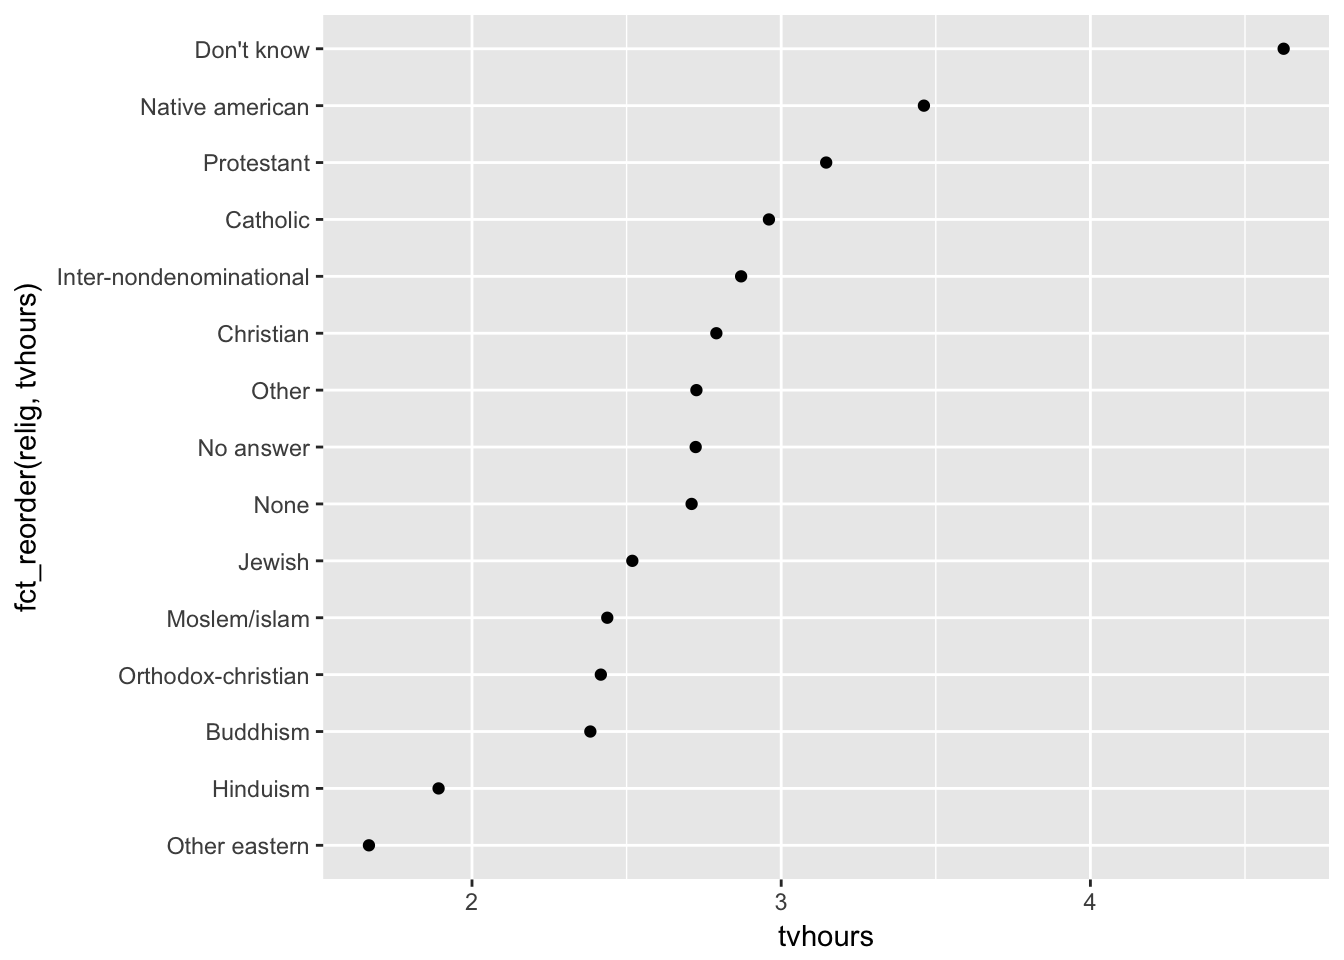
\includegraphics{main_files/figure-latex/unnamed-chunk-144-1.pdf}

\textbf{Joonis 2. See jaotus iseloomustab keskmise ES paiknemist puhtalt
meie andmete põhjal.}

Täpsemalt, selle joonise põhjal võib arvutada, milline on meie valimi
keskväärtuse kohtamise tõenäosus igal võimalikul tõelisel ES-i
väärtusel. Kõige tõenäolisemad on andmed siis, kui tegelik ES = andmete
keskväärtusega (seda kohta näitab must joon). Kui me jagame musta joone
pikkuse punase kurvi all läbi katkendjoone pikkusega sama kurvi all,
saame teada, mitu korda on meie andmed tõenäolisemad siis, kui tegelik
ES = mean(valimi ES), võrreldes olukorraga, kus tegelik ES = 0.
Loomulikult võime sama näitaja arvutada ükskõik millise hüpoteeside
paari kohta (näiteks, andmed on miljon korda tõenäolisemad hüpoteesi ES
= 0.02 all kui hüpoteesi ES = -1 all; mis aga ei tähenda, et andmed
oleksid väga tõenäolised kummagi võrreldud hüpoteesi all).

Aga see ei ole veel Bayes. Lisame andmemudelile taustateadmiste mudeli.
Sellega tühistame me väga olulise eelduse, mis ripub veskikivina
sagedusliku statistika kaelas. Nimelt, et valimi andmed peavad olema
esinduslikud populatsiooni suhtes. Me võime olla üsna kindlad, et
väikeste valimite korral see eeldus ei kehti ja sellega seoses ei tööta
ka sageduslik statistika viisil, milleks R.A. Fisher selle kunagi lõi.
Taustateadmiste mudeli roll (kuigi mitte ainus) on õrnalt suunata meie
hinnangut õiges suunas vähendades halbade andmete võimet meile kahju
teha. Kui sul on väike valim, siis sinu andmed vajavad sellist
kantseldamist.

Olgu meie taustateadmise mudel normaaljaotus keskväärtusega 0 ja
standardhälbega 1

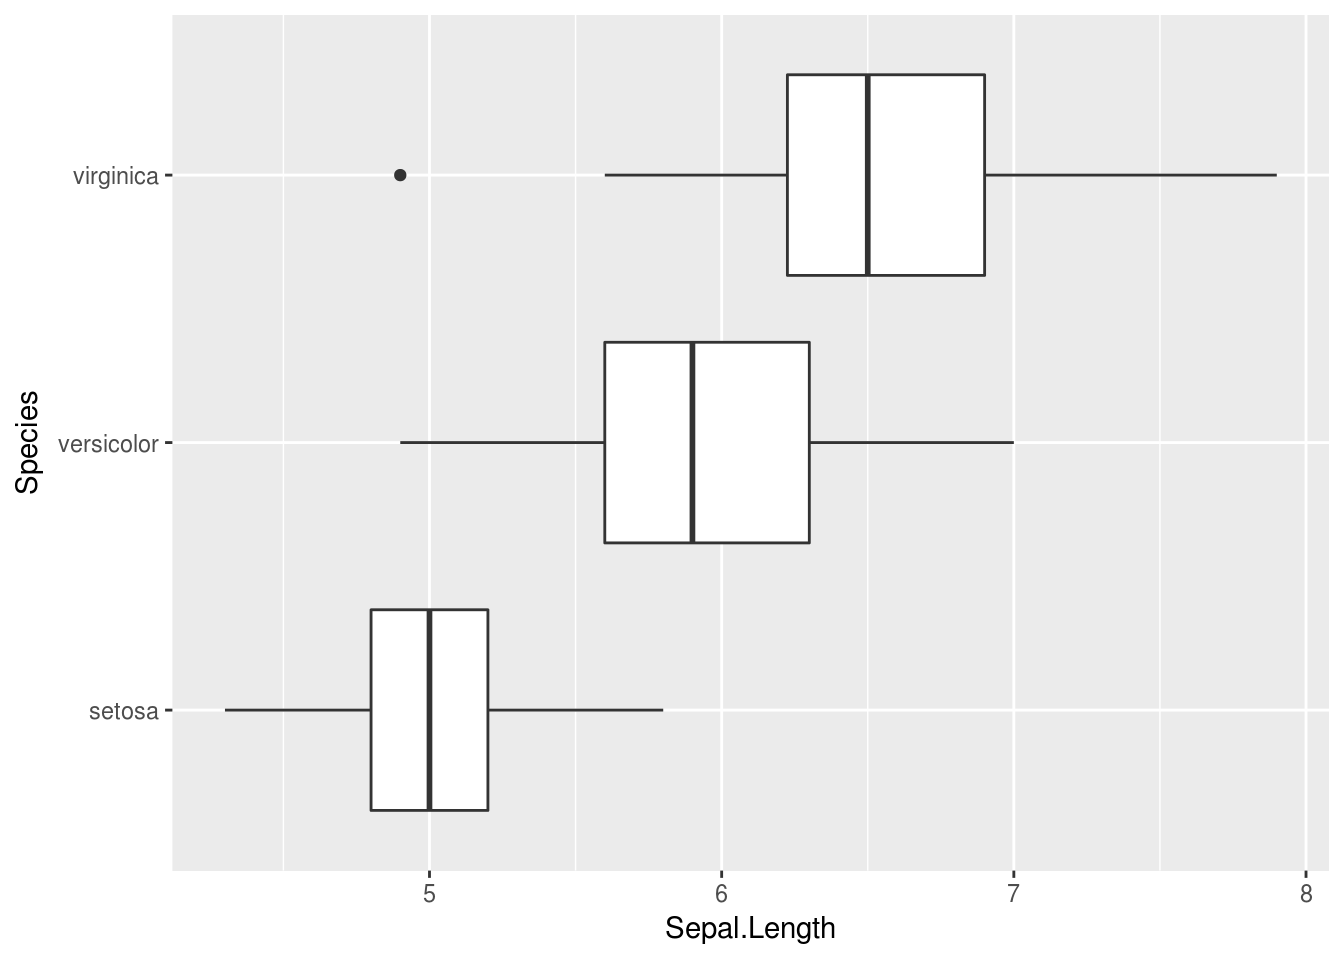
\includegraphics{main_files/figure-latex/unnamed-chunk-145-1.pdf}

\textbf{Joonis 3. Taustateadmiste mudel e prior on must normaaljaotus,
mille ülesanne on veidi vähendada ekstreemsete valimite kahjulikku
mõju.}

Taustateadmiste mudel on sageli normaaljaotus. Kui meil on palju
taustateadmisi, siis on see jaotus kõrge ja kitsas, kui meil on vähe
taustateadmisi, siis on see madal ja lai.

\begin{verbatim}
  Mida teha, kui sa ei taha, et taustateadmiste mudel sinu 
  posteeriori kuju mõjutab? Sellisel juhul kasutatakse nõrgalt 
  informatiivseid prioreid, mis tähendab, et priori 
  jaotus on palju laiem kui tõepäramudeli laius. Miks mitte 
  kasutada mitte-informatiivseid tasaseid prioreid? 
  Põhjused on arvutuslikud, seega tehnilist laadi.
\end{verbatim}

Igal juhul järgmise sammuna korrutab bayesiaan selle jaotuse
andmejaotusega, saades tulemuseks kolmanda normaaljaotuse, mille ta
seejärel normaliseerib nii, et jaotuse alune pindala = 1. See kolmas
jaotus on posterioorne tõenäosusjaotus, mis sisaldab kogu infot, millest
saab arvutada kõige tõenäolisema katseefekti suuruse koos ebakindluse
määraga selle ümber (mida rohkem andmeid, seda väiksem ebakindlus) ja
tõenäosused, et tegelik katseefekt jääb ükskõik milllisesse meid
huvitavasse vahemikku.

Nüüd ei ole siis muud kui bayesi mudel läbi arvutada.

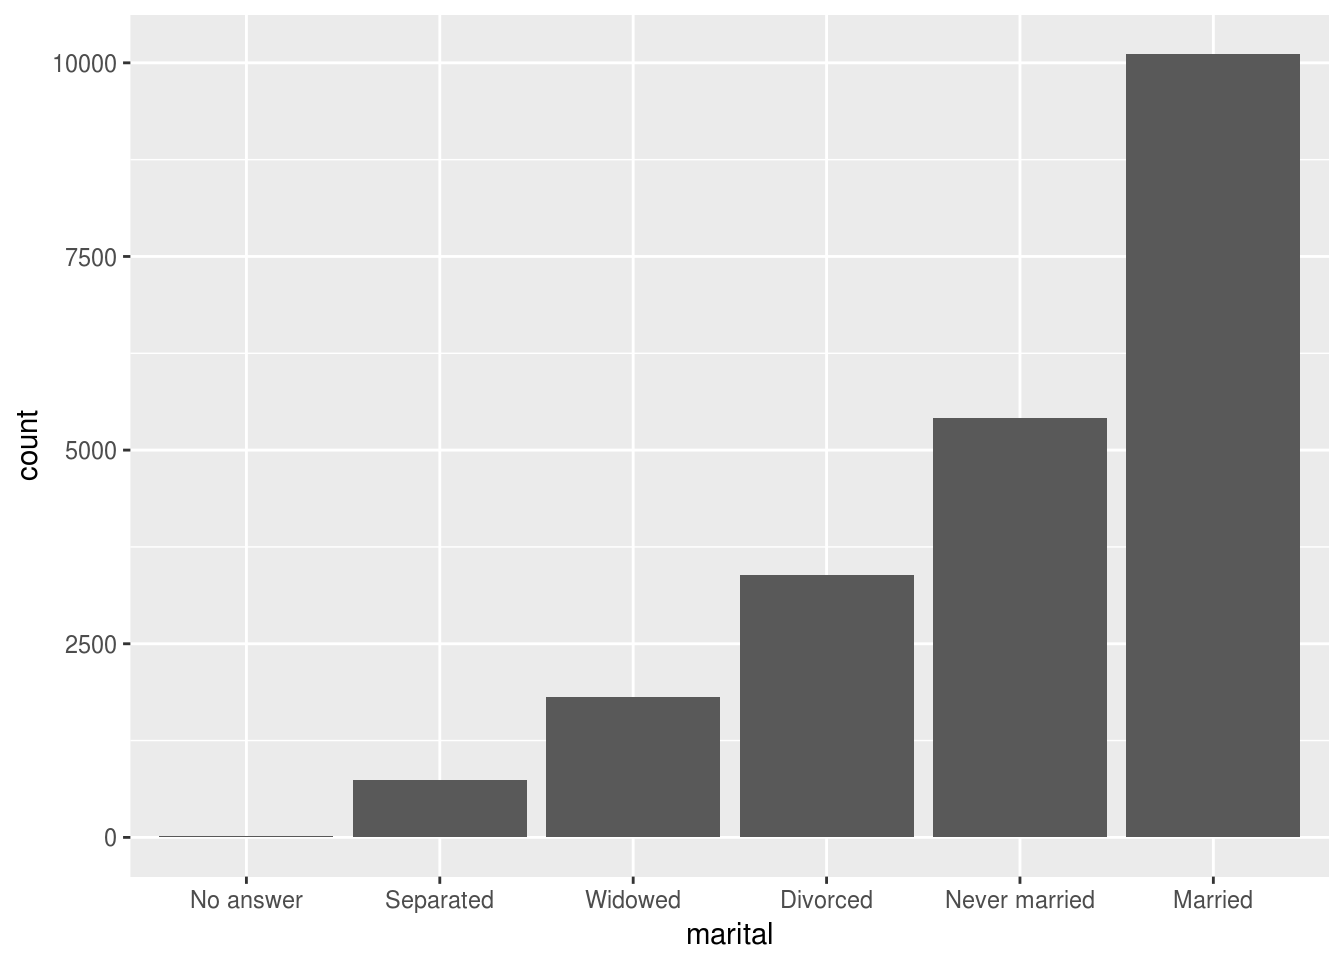
\includegraphics{main_files/figure-latex/unnamed-chunk-147-1.pdf}

\textbf{Joonis 4. Triplot. Bayesi väljund on posterioorne
tõenäosusjaotus (roheline). Nagu näha, ei ole selle jaotuse tipp täpselt
samas kohas kui andmejaotuse tipp ehk keskväärtus. Prior tõmbab seda
veidi nulli suunas. Lisaks on posteerior veidi kitsam kui andmemudel,
mis tähendab, et hinnang ES-le tuleb väiksema ebakindluse määraga.}

Posteerior sisaldab endas kogu infot, mis meil ES-i tõelise väärtuse
kohta on. Siit saame arvutada

\begin{enumerate}
\def\labelenumi{\arabic{enumi}.}
\item
  parima hinnangu ES-i punktväärtusele,
\item
  usaldusintervalli, ehk millisest ES-ide vahemikust loodame leida
  tõelise ES-i näit 90\% tõenäosusega,
\item
  iga mõeldava ES-i väärtuste vahemiku kohta tõenäosuse, millega tõeline
  ES jääb sellesse vahemikku.
\item
  saame ES-i põhjal arvutada mõne muu statistiku, näiteks ES1 = log(ES),
  kasutades selleks ES-i posterioorset jaotust. Sel viisil kanname oma
  ES-i hinnangus peituva ebakindluse üle ES1-le, millele saame samuti
  rakendada punkte 1-3 (sest ES1 on posterioorne jaotus).
\item
  uute andmete lisandumisel saame kasutada ES-i posteeriorit uue
  priorina ja arvutada uue täiendatud posteeriori. Põhimõtteliselt võime
  seda teha pärast iga üksiku andmepunkti lisandumist. See avab ka head
  võimalused metaanalüüsiks.
\item
  lisaks saame oma algsest mudelist ka posteeriori andmepunkti tasemel
  varieeruvusele (pole näidatud). Seda kasutame uute andmete
  simuleerimiseks (meie näites üksikud ES-d).
\end{enumerate}

\subsubsection{Sageduslik statistik}\label{sageduslik-statistik}

Sageduslik lähenemine sisaldab ainult ühte mudelit, mida võrreldakse
valimi andmetega. Sageduslik statistik alustab selles lihtsas näites
täpselt samamoodi nagu bayesiaan, tekitades eelmisega identse
andmemudeli, mis on keskendatud valimi keskväärtusele (Joonis 2).
Seejärel nihutab ta oma andmemudelit niipalju, et normaaljaotuse tipp ei
ole enam valimi keskväärtuse kohal vaid hoopis 0-efekti kohal. Jaotuse
laius nihutamisel ei muutu.

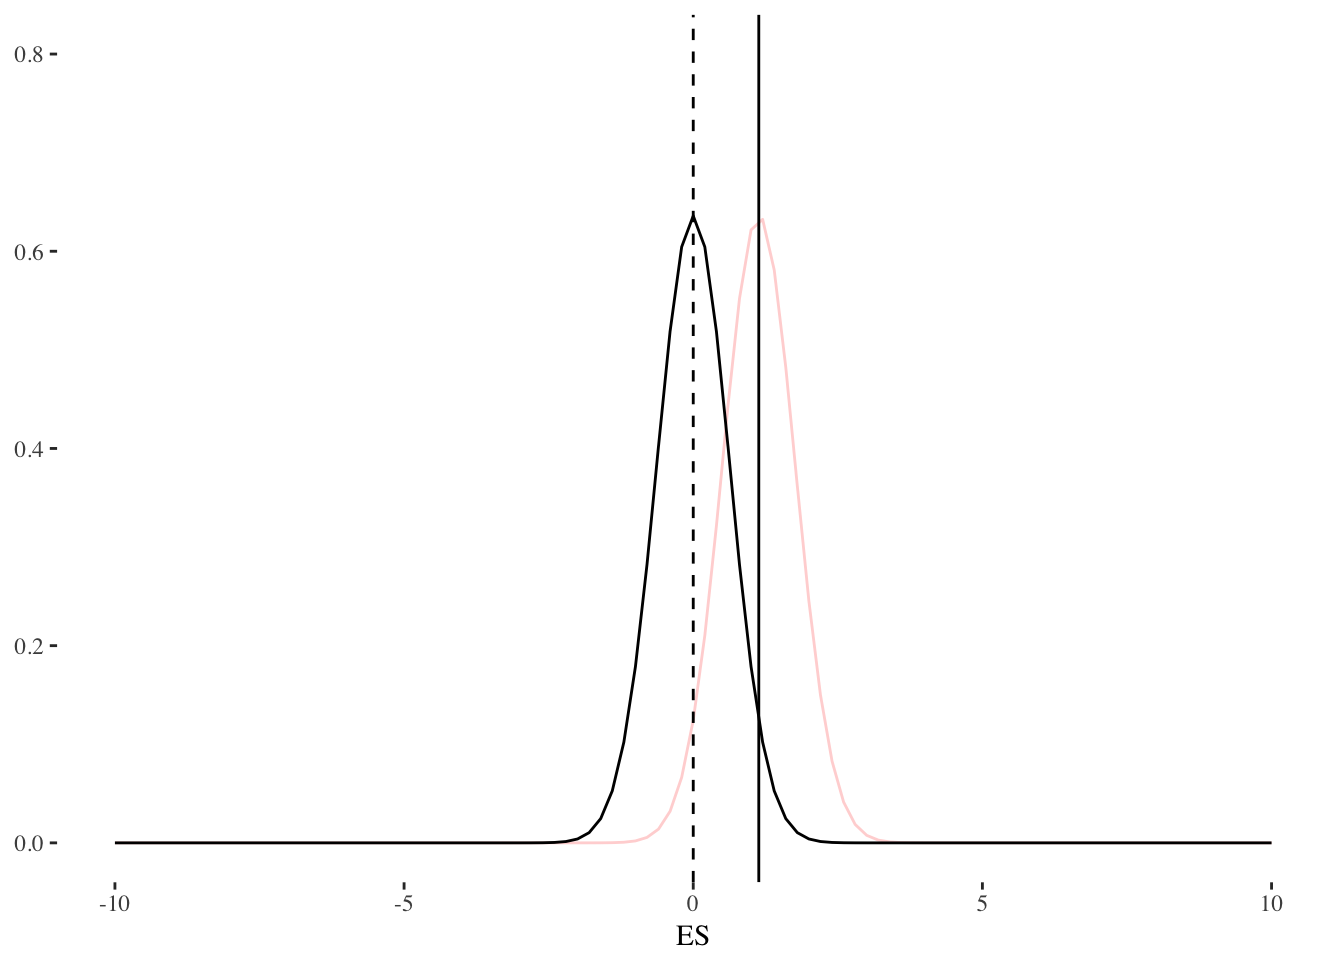
\includegraphics{main_files/figure-latex/unnamed-chunk-148-1.pdf}

Seda nullile tsentreeritud mudelit kutsutakse null-hüpoteesiks (H0).
Nüüd võrdleb ta oma valimi keskväärtust (must joon) H0 jaotusega. Kui
valimi keskväärtuse kohal on H0 jaotus kõrge, siis on andmete tõenäosus
H0 kehtimise korral suur. Ja vastupidi, kui valimi keskväärtuse kohal on
H0 madal, siis on andmete esinemise tõenäosus H0 all madal. Seda
tõenäosust kutsutakse p väärtuseks. Mida väiksem on p, seda vähem
tõenäolised on teie andmed juhul, kui H0 on tõene ja katseefekt võrdub
nulliga. P on defineeritud kui ``teie andmete või 0-st veel kaugemal
asuvate andmete esinemise pikaajaline suhteline sagedus tingimusel, et
H0 kehtib''.

\subsubsection{tulemuste tõlgendamine}\label{tulemuste-tolgendamine}

Kui sageduslik statistik kirjutab, et tema ``efekti suurus on
statistiliselt oluline 0.05 olulisusnivool'', siis ta ütleb sellega, et
tema poolt arvutatud p \textless{} 0.05. Selle väite korrektne tõlgendus
on, et juhul kui statistik pika aja jooksul võtab omaks ``statistiliselt
olulistena'' kõik tulemused, millega kaasnev p \textless{} 0.05 ja
lükkab tagasi kõik tulemused, mille p \textgreater{} 0.05, siis sooritab
ta 5\% sagedusega tüüp 1 vigu. See tähendab, et igast sajast tõesest
H0-st, mida ta testib, võtab ta keskeltläbi 5 vastu, kui statistiliselt
olulised. Sageduslik statistika on parim viis tüüp 1 vigade sageduse
pikaajaliseks fikseerimiseks. Paraku ei tea me ühegi üksiku testi kohta
ette, kas see testib kehtivat või mittekehtivat H0-i, mis teeb raskeks
katseseeriate ühekaupa tõlgendamise. Tuletame meelde, et sageduslikus
statistikas ei saa rääkida H0 kehtimise tõenäosusest vaid peab rääkima
andmete tõenäosusest (ehk andmete esinemise sagedusest) tingimusel, et
H0 kehtib.

\textbf{Kas ühte p väärtust saab tõlgendada kui hinnangut
tõendusmaterjali hulgale, mida teie valim pakub H0 vastu?} Selle üle on
vaieldud juba üle 80 aasta, kuid tundub, et ainus viis seda kas või
umbkaudu teha on bayesiaanlik. Igal juhul, p väärtust, mis on
defineeritud pikaajalise sagedusena, on raske rakendada üksiksündmusele.
Bayesiaanliku p väärtuste tõlgendamiskalkulaatori leiate aadressilt
\url{http://www.graphpad.com/quickcalcs/interpretPValue1/}

\begin{verbatim}
Kujutle mass spektroskoopia katset, kus mõõdame 2000 valgu 
tasemeid katse-kontroll skeemis ja katset korratakse n korda. 
Sageduslik statistik kasutab adjusteeritud p väärtusi või q 
väärtusi, et tõmmata piir, millest ühele poole jäävad statistiliselt 
olulised ES-d ja teisele poole mitteolulised null-efektid. Edasi 
tõlgendab ta mitteolulisi efekte kui ebaolulisi ja diskuteerib vaid 
"olulisi" efekte. Paraku, p väärtuste arvutamine ja adjusteerimine 
saab toimuda mitmel erineval moel ja usalduspiiri panekule just 95-le 
protsendile, mitte näiteks 89% või 99.2%-le, pole ühtegi ratsionaalset 
põhjendust. Seega tõmbab ta sisuliselt juhuslikus kohas joone läbi 
efektide, misjärel ignoreerib kõiki sellest joonest valele poole jäänud 
efekte. Meetod, mis väga hästi töötab pikaajalises kvaliteedikontrollis, 
ei ole kahjuks kuigi mõistlik katse tulemuste ükshaaval tõlgendamises. 
Mis juhtub, kui oleme kavalad ja proovime mitmeid erinevaid p väärtustega 
töötamise meetodeid, et valida välja see usalduspiir, millest õigele poole 
jäävaid andmeid on teaduslikult kõige parem tõlgendada? Ehkki ükshaaval 
võisid kõik meie poolt läbi arvutatud meetodid olla lubatud (ja isegi 
võrdselt head), ei fikseeri p enam tüüp 1 vigade sagedust. See tähendab, 
et p on kaotanud definitsioonijärgse tähenduse ja te oleksite võinud oma 
olulisuspiiri sama hästi tõmmata tunde järgi.
\end{verbatim}

tüüpiline tulemuse kirjeldus artiklis:

\begin{enumerate}
\def\labelenumi{\arabic{enumi}.}
\item
  sageduslik: the effect is statistically significant (p \textless{}
  0.01).
\item
  bayesiaanlik: the most likely effect size is q1 (90\% CI = q2, q3) and
  the probability that the true effect is \textless{} 0 is q4 percent.
\end{enumerate}

90\% CI --- credible interval --- tähendab, et me oleme 90\% kindlad, et
tegelik efekti suurus asub vahemikus q2 \ldots{} q3.

\subsubsection{kahe paradigma
erinevused}\label{kahe-paradigma-erinevused}

\begin{enumerate}
\def\labelenumi{\arabic{enumi}.}
\item
  sageduslikus statistikas võrdub punkt-hinnang tegelikule efekti
  suurusele valimi keskmise ES-ga. Bayesi statistikas see sageli nii ei
  ole, sest taustateadmiste mudel mõjutab seda hinnangut. Paljud mudelid
  püüavad ekstreemseid valimeid taustateadmiste abil veidi mõistlikus
  suunas nihutada, niiviisi vähendades ülepaisutatud efektide avaldamise
  ohtu.
\item
  sageduslik statistika töötab tänu sellele, et uurija võtab vastu
  pluss-miinus otsuseid: iga H0 kas lükatakse ümber või jäetakse
  kehtima. Seevastu bayesiaan mõtleb halli varjundites: sissetulevad
  andmed kas suurendavad või vähendavad hüpoteeside tõenäosusi (mis
  jäävad aga alati \textgreater{} 0 ja \textless{} 1).
\item
  p väärtused kontrollivad tüüp 1 vigade sagedust ainult siis, kui katse
  disaini ja hilisema tulemuste analüüsi detailid on enne katse
  sooritamist jäigalt fikseeritud (või eelnevalt on täpselt paika pandud
  lubatud variatsioonid katse- ja analüüsi protokollis). Eelkõige
  tähendab see, et valimi suurus ja kasutatavad statistilinsed testid
  peavad olema eelnevalt fikseeritud. Tüüpiliselt saame p väärtuse
  arvutada vaid üks kord ja kui p = 0.051, siis oleme sunnitud H0 paika
  jätma ning efekti deklareerimisest loobuma. Me ei saa lihtsalt katset
  juurde teha, et vaadata, mis juhtub. Bayesiaan seevastu võib oma
  posterioorse tõenäosuse arvutada kasvõi pärast iga katsepunkti
  kogumist ning katse peatada kohe (või alles siis), kui ta leiab, et
  tema posterioorne jaotus on piisavalt kitsas, et teaduslikku huvi
  pakkuda.
\item
  sagedusliku statistika pluss-miinus iseloom tingib selle, et kui
  tegelik efekti suurus on liiga väike, et sattuda õigele poole
  olulisusnivood, siis annavad statistiliselt olulisi tulemusi
  ülepaisutatud efektid, mida tekib tänu valimiveale. Nii saab
  süstemaatiliselt kallutatud teaduse. Bayesi statistikas seda probleemi
  ei esine, kuna otsused ei ole pluss-miinus tüüpi.
\item
  bayesi statistika ei fikseeri tüüp 1 vigade sagedust. See-eest võitleb
  see nn valehäirete vastu, milleks kaasajal kasutatakse enim
  hierarhilisi shrinkage mudeleid. See on bayesi vaste sageduslikus
  statistikas kasutatavatele multiple testingu korrektsioonidele. Kui
  sageduslik statistik võitleb valehäiretega p väärtusi adjusteerides ja
  selle läbi olulisusnivood nihutades, siis bayesiaan kasutab shrinkage
  mudelit, et parandada hinnanguid üksikute efektide keskväärtustele ja
  nende sd-le, kasutades paindlikult kogu andmesetis leiduvat infot.
\end{enumerate}

See on kõik, mida me sagedusliku statistika kohta ütleme. Mitte miski,
mis järgneb, ei eelda sagedusliku paradigma tundmist.

\chapter{1. osa: Mudel ja maailm}\label{osa-mudel-ja-maailm}

Andmeanalüüs ja statistika (siin sünonüümid) on lahutamatu osa igast
loodusteadusest. Järgnevalt seletan, miks.

\subsection{Suur ja väike maailm}\label{suur-ja-vaike-maailm}

Kuna maailm on liiga suur ja keeruline, et seda otse uurida, lõikavad
teadlased selle väiksemateks tükkideks, kasutades tordilabidana
teaduslike hüpoteese. Tüüpiline hüpotees pakub välja mittematemaatilise
seletuse mõnele kitsalt piiritletud loodusnähtusele. Näiteks
darvinistlik evolutsiooniteooria püüab seletada evolutsiooni
toimemehhanisme. Seda teooriat võib võrrelda empiiriliste andmetega.

Mis juhtub, kui teie lemmikhüpotees on andmetega kooskõlas? Kas see
tähendab, et see hüpotees on tõene? Või, et see on tõenäoliselt tõene?
Kahjuks on vastus mõlemale küsimusele eitav. Põhjuseks on asjaolu, et
enamasti leiab iga nähtuse seletamiseks rohkem kui ühe alternatiivse
teadusliku hüpoteesi (näit. lamarksistlik evolutsiooniteooria) ning
rohkem kui üks üksteist välistav hüpotees võib olla olemasolevate
andmetega võrdses kooskõlas. Asja teeb veel hullemaks, et teoreetiliselt
on võimalik sõnastada lõpmatult palju erinevaid teooriaid, mis kõik
pakuvad alternatiivseid ja üksteist välistavaid seletusi samale
nähtusele.

Olgu peale, kui me vaatame maailma kõiketeadja jumala perspektiivist,
siis tema võib vaadelda kõikehõlmava tõendusmaterjali sobivust kõigi
võimalike teooriatega ning valida välja selle ainsa teooria, mis kõige
paremini tõendusmaterjaliga sobib. Kuigi, see eeldaks, et tal on lõpmata
palju andmeid, sest muidu ei oleks tal loogiliselt võimalik lõpmata
paljude teooriate vahel valida - aga jumala jaoks on kõik võimalik. Igal
juhul meie, surelike, jaoks tähendab see, et teaduslikus ``faktis'' saab
alati kahelda, sest kunagi ei või kindel olla, et parimad teooriad
lõpmata suurest teooriapilvest ei ole meil täiesti tähelepanuta jäänud
ning, et meie jaoks eksisteerivad andmed kajastaksid hästi kõiki
võimalikke andmeid. On selge nagu seebivesi, et mida vähem aega me
kulutame teoorialoomeks ja andmete kogumiseks, seda vähem usutavad on ka
meie teaduslikud järeldused. Sageli on nii, et mida kehvem on olukord
andmerindel, seda rohkem vajame statistikat. Kui meil õnnestuks oma
andmetest ilma statistikata saia teha, ei kõhkleks me hetkegi! Eriti,
kuna statistikaga käivad käsikäes statistilised mudelid.

\subsection{Mudeli väike maailm}\label{mudeli-vaike-maailm}

Ülalmainitud teadusliku meetodi puudused tingivad, et meie huvides on
oma teaduslikke probleeme veel ühe taseme võrra lihtsustada, taandades
need statistilisteks probleemideks. Selleks tuletame me tavakeelsest ja
laiahaardelisest teaduslikust teooriast täpselt formuleeritud
matemaatilise mudeli ning seejärel asume uurima oma mudelit.

Mudeli maailm erineb päris maailmast selle poolest, et mudeli maailmas
on kõikvõimalikud sündmused, mis põhimõtteliselt võivad juhtuda, juba
ette teada ja üles loetud (seda sündmuste kogu kutsutakse
parameetriruumiks). Seega, tehniliselt on mudeli maailmas üllatused
võimatud.

Mudeli eeliseks teooria ees on, et hästi konstrueeritud mudel on
lihtsamini mõistetav --- erinevalt vähegi keerulisemast teaduslikust
hüpoteesist on mudeli eeldused ja ennustused läbinähtavad ja täpselt
formuleeritavad. Mudeli puuduseks on aga, et erinevalt teooriast ei ole
mingit võimalust, et mudel vastaks tegelikkusele ehk oleks tõene. Seda
sellepärast, et mudel on taotluslikult lihtsustav (erandiks on puhtalt
ennustuslikud mudelid, mis on aga enamasti läbinähtamatu struktuuriga).
Mudel on kas kasulik või kasutu; teooria on kas tõene või väär. Mudeli
ja maailma vahel võib olla kaudne ``peegeldus'', aga mitte kunagi otsene
side. Seega, ükski number, mis arvutatakse mudeli raames, ei kandu sama
numbrina üle teaduslikku ega päris maailma. Ja kogu statistika (ka
mitteparameetriline) toimub mudeli väikses maailmas. Arvud, mida
statistika teile pakub, elavad mudeli maailmas; samas kui teie teaduslik
huvi on suunatud päris maailmale. Näiteks 95\% usaldusintervall ei
tähenda, et te peaksite olema 95\% kindel, et tõde asub selles
intervallis -- sageli ei tohiks te seda nii julgelt tõlgendada isegi
kitsas mudeli maailmas.

\subsubsection{Näide: Aristoteles, Ptolemaios ja
Kopernikus}\label{naide-aristoteles-ptolemaios-ja-kopernikus}

Aristoteles lõi teooria maailma toimimise kohta, mis domineeris haritud
Eurooplase maailmapilti enam kui 1200 aasta vältel. Selle kohaselt asub
universumi keskpunktis maakera ning kõik, mida siin leida võib, on
tehtud neljast elemendist: maa, vesi, õhk ja tuli. Samas, kogu
maailmaruum alates kuu sfäärist on tehtud viiendast elemendist (eeter),
mida aga ei leidu maal (nagu nelja elementi ei leidu kuu peal ja sealt
edasi). Taevakehad (kuu, päike, planeedid ja kinnistähed) tiirlevad
ümber maa kontsentrilistes sfäärides, mis on omavahel seotud (mille
vahel pole vaba ruumi). Seega on kogu liikumine eetri sfäärides ühtlane
ja ringikujuline ja see liikumine põhjustab pika põhjus-tagajärg ahela
kaudu kõiki liikumisi, mida maapeal kohtame. Kaasa arvatud meie
sündimine, elukäik ja surm (mis on kõik liikumised). Kõik, mis maapeal
huvitavat, ehk kogu liikumine, on algselt põhjustatud esimese liikumise
poolt, mille käivitab kõige välimises sfääris paiknev meie jaoks
mõistetamatu intellektiga ``olend''.

Aristotelese suur teooria ühendab kogu maailmapildi alates kaasaegses
mõistes keemiast ja kosmoloogiast kuni bioloogia, maateaduse ja isegi
geograafiani. Sellised ühendteooriad on nagu 500 aastased sekvoiad; nad
on rasked langetada, aga kui mõni siiski kukub, kostab ragin kaugele.
Samas, ühte Aristotelese kosmoloogia olulist puudust nähti kohe. Nimelt
ei suuda Aristoteles seletada, miks osad planeedid teavavõlvil vahest
suunda muudavad ja mõnda aega lausa vastupidises suunas liiguvad
(retrogressioon). Kuna astronoomia põhiline kasutusala oli astroloogia,
siis põõrati planeetide liikumisele suurt tähelepanu. Lahenduseks ei
olnud aga mitte suure teooria ümbertegemine või ümberlükkamine, vaid
nõudlus uue teaduse järele, mis ``päästaks fenomenid''. Siin tuli appi
Ptolemaios, kes lõi matemaatilise mudeli, kus planeedid mitte lihtsalt
ei liigu ringtrajektoori mõõda vaid samal ajal teevad ka väiksemaid
ringe ümber esimese suure ringjoone. Neid väiksemaid ringe kutsutakse
epitsükliteks. See mudel suutis planeetide liikumist taevavõlvil
piisavalt hästi ennustada, et astroloogide nõudlik seltskond sellega
rahule jäi.

Ptolemaiosel ja tema järgijatel oli tegelikult mitu erinevat mudelit.
Osad neist ei sialdanud epitsükleid ja maakera ei asunud tema mudelites
universumi keskel, vaid oli sellest punktist eemale nihutatud --- nii et
päike ei teinud ringe ümber maakera vaid ümber tühja punkti. On oluline,
et leidus epitsüklitega mudel ja ilma epitsükliteta mudel, mis olid
matemaatiliselt ekvivalentsed ja seega andsid võrdseid ennustusi. Oli
selge, et Aristotelese teooria ja fenomenide päästmise mudelid olid
fundamentaalselt erinevad asjad. Samal ajal kui Aritoteles
\textbf{seletas} maailma põhiolemust põhjuslike seoste jadana (mitte
matemaatiliselt), \textbf{kirjeldas/ennustas} Ptolemaios sellesama
maailma käitumist matemaatiliste (mitte põhjuslike) struktuuride abil.

Nii tekkis olukord, kus maailma mõistmiseks kasutati 1000 aasta vältel
Aristotelese ühendteooriat aga selle kirjeldamiseks ja tuleviku
ennustamiseks hoopis ptolemailisi mudeleid, mida keegi päriselt tõeks ei
pidanud ja mida hinnati selle järgi, kui hästi need ``päästsid
fenomene''.

See toob meid Koperniku juurde, kes teadusajaloolaste arvates vallandas
17. sajandi teadusliku revolutsiooni avaldades raamatu, kus ta asetab
päikese universumi keskele ja paneb maa selle ümber ringtrajektooril
tiirlema. Kas Kopernikus tõrjus sellega kõrvale Aristotelese,
Ptolemaiose või mõlemad? Kaasaegne seisukoht on, et kuigi Kopernikus
soovis teha kolmandat, arvasid tema rängalt matemaatilise teose
avaldamisele järgnenud 40 aasta vältel pea kõik asjatundlikud
astronoomid, et ta soovis välja pakkuda vaid lihtsama alternatiivi
epitsüklitega mudelile, mis selleks ajaks oli muutunud väga keerukaks
(aga ka samavõrra ennustustäpseks). Kuna Kopernikuse raamat läks trükki
ajal, mil selle autor oli juba surivoodil, kirjutas sellele eessõna üks
tema vaimulikust sõber, kes püüdis oodatavat kiriklikku pahameelt
leevendada sugereerides, et päikese keskele viimine ei ole muud kui
mudeldamise trikk, millest ei tasu järeldada, et maakera ka tegelikult
ümber päikese tiirleb (piibel räägib, kuidas jumal peatas taevavõlvil
päikese, mitte maa). Ja kuna eessõna oli anonüümne, eeldasid lugejad
muidugi, et selle kirjutas autor. Lisaks, kuigi Kopernikus tõstis
päikese keskele, jäi ta ringikujuliste trajektooride juurde, mis
tähendas, et selleks, et tema mudel fenomenide päästmisel hätta ei jääks
ja astroloogidele kasutu ei oleks, oli ta sunnitud maad ja planeete
liigutama ümber päikese mõõda epitsükleid. Kokkuvõttes oli Koperniku
mudel sama keeruline kui Ptolemaiose standardmudel (neis oli võrdne arv
epitsükleid) ja selle abil tehtud ennustused planeetide liikumise kohta
olid väiksema täpsusega.

\begin{verbatim}
  Koperniku mudel suutis samas ennustada mõningaid nähtusi (planeetide näiv
  heledus muutub ning jõuab maksimumi nende lähimas asukohas maale), mida
  Ptolemaiose mudel ei ennustanud. See ei tähenda, et need fenomenid oleksid
  olnud vastuolus Ptolemaiose mudeliga. Lihtsalt, nende Ptolemaiose mudelisse
  sobitamiseks oli vaja osad mudeli parameetrid fikseerida nii-öelda suvalistele väärtustele. 
  Seega Koperniku mudel töötas nii, nagu see oli, samas kui Ptolemaiose mudel vajas ad hoc tuunimimst.  
\end{verbatim}

Kui vaadata Koperniku produkti teooriana, mitte mudelina, siis oli sel
selgeid eeliseid Aristotelese ees. Juba ammu oli nähtud komeete üle
taevavõlvi lendamas (mis Aristotelese järgi asusid kinnistähtede
muutumatus sfääris) ja supernoova tekkimist ja kadu, ning enam ei olnud
kaugel ka aeg mil Galileo joonistas oma teleskoobist kraatreid kuu
pinnal, näidates, et kuu ei saanud koosneda täiuslikust viiendast
elemendist ja et sellel toimusid ilmselt sarnased füüsikalised
protsessid kui maal. On usutav, et kui Kopernikus oleks jõudnud oma
raamatule ise essõna kirjutada, oleks tema teooria vastuvõtt olnud palju
kiirem (ja valulisem). Seega, teooria ja mudeli eristus on tähtis!

\begin{verbatim}
  Koperniku teooriast tuleneb loogilise paratamatusena, et tähtedel esineb
  maapealt vaadates parallaks. See tähendab, et kui maakera koos astronoomiga
  teeb poolringi ümber päikese, siis kinnistähe näiv asukoht taevavõlvil
  muutub sest astronoom vaatleb teda teise nurga alt. Pange oma nimetissõrm
  näost u 10 cm kaugusele, sulgege parem silm, seejärel avage see ning sulgege
  vasak silm ja te näete oma sõrme parallaksi selle näiva asukoha muutusena.
  Tähtede parallaksi püüti mõõta juba Aleksandrias 1000 aastat enne Kopernikust, 
  et leida kinnitust teooriale, mille kohaselt maakera tiirleb ümber päikese. 
  Mõõtmised ei näidanud aga parallaksi olemasolu (sest maa trajektoori diameeter 
  on palju lühem kui maa kaugus tähtedest). Parallaks mõõdeti edukalt alles 1838, 
  siis kui juba ammu iga koolijüts uskus, et maakera tiirleb ümber päikese!
  
  
\end{verbatim}

\subsection{Millest koosneb mudel?}\label{millest-koosneb-mudel}

\begin{quote}
Mudel on matemaatilise formalism, mis püüab kirjeldada füüsikalist
protsessi. mudeli struktuuris on komponent, mis kirjeldab ideaalseid
ennustusi ja eraldi veakomponent, mis kirjeldab kuidas andmepunktid
varieeruvad selle ideaalse ennustuse ümber.
\end{quote}

Näiteks, sageli kirjeldame me produkti kuhjumist ensüümreaktsioonis
eksponentsiaalse funktsioni (mudeli) abil. Kui meie andmed seda tüüpi
funktiooniga sobivad, ütleb see meile midagi konkreetse ensüümi
töömehhanismi kohta. Teisest küljest, need mudelid, mis on
``generatiivsed'', suudavad lisaks simuleerida ka uusi andmeid.
Sealhulgas ka selliseid, mida päris maailmas ei saa kunagi esineda, sest
seal puuduvad vastavad tingimused. Mudelisse saab aga sisse kirjutada
igasuguseid tingimusi ehk parameetri väärtusi (näit substraadi
konsentratsioone, mida me ei suuda ``päriselt'' saavutada).

Oletame, et me mõõtsime N inimese pikkuse cm-s ja kaalu kg-s ning meid
huvitab, kuidas inimeste pikkus sõltub nende kaalust. Lihtsaim mudel
pikkuse sõltuvusest kaalust on pikkus = kaal (formaliseeritult: y = x)
ja see mudel ennustab, et kui Johni kaal = 80 kg, siis John on 80 cm
pikkune. Selle mudeli saame graafiliselt kujutada nii

\begin{Shaded}
\begin{Highlighting}[]
\NormalTok{x <-}\StringTok{ }\DecValTok{50}\OperatorTok{:}\DecValTok{200} \CommentTok{#y = kaal}
\NormalTok{y <-}\StringTok{ }\NormalTok{x }\CommentTok{# x = pikkus }
\KeywordTok{plot}\NormalTok{(y}\OperatorTok{~}\NormalTok{x, }\DataTypeTok{type=}\StringTok{"l"}\NormalTok{, }\DataTypeTok{xlab=}\StringTok{"weight in kg"}\NormalTok{, }\DataTypeTok{ylab=}\StringTok{"heigth in cm"}\NormalTok{, }\DataTypeTok{main=}\StringTok{"fixed linear model"}\NormalTok{)}
\end{Highlighting}
\end{Shaded}

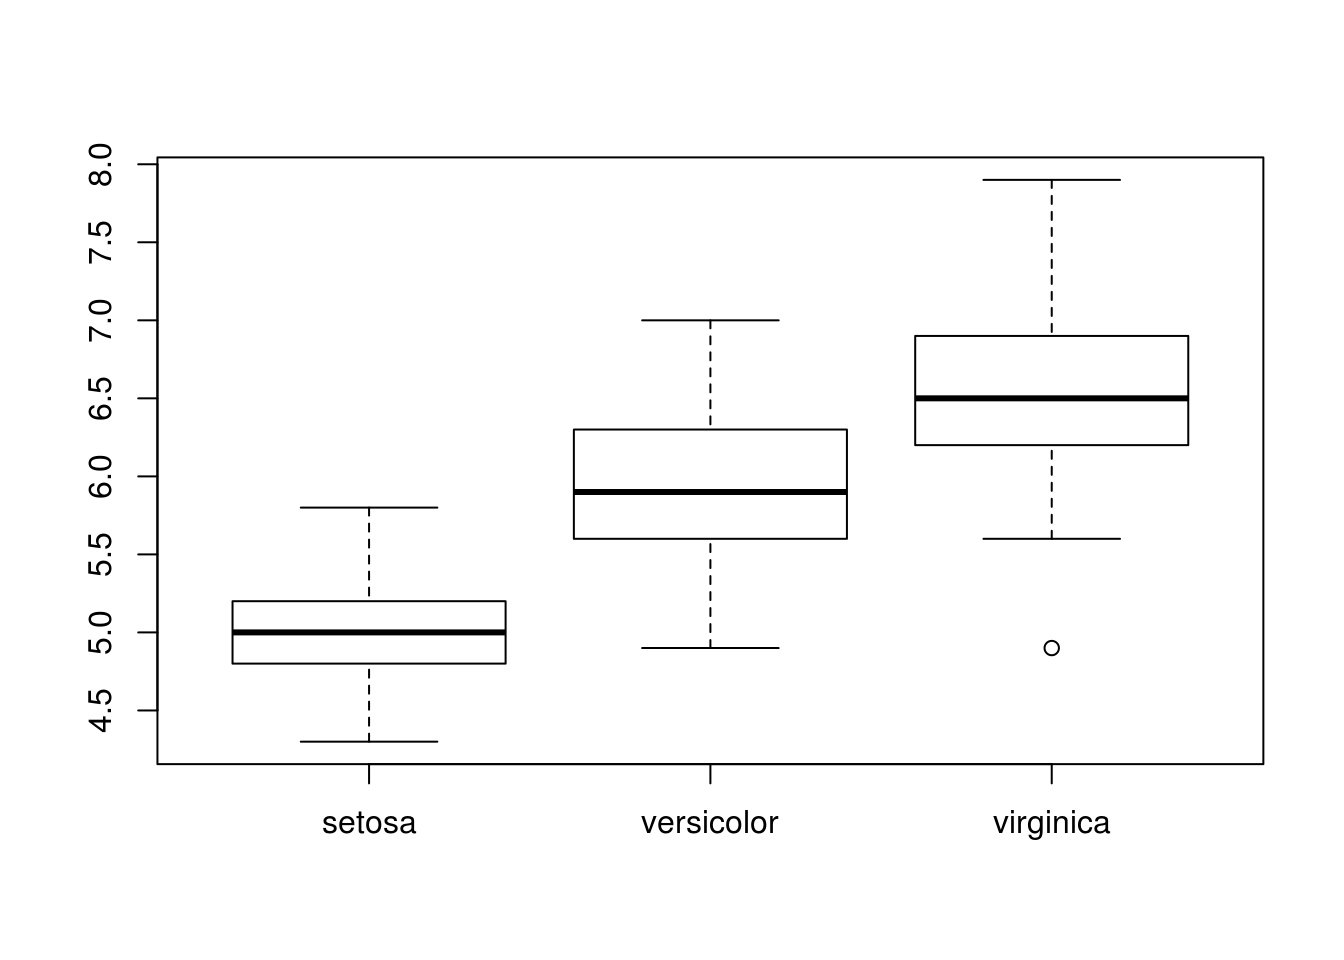
\includegraphics{main_files/figure-latex/unnamed-chunk-149-1.pdf}

kõigepealt painutame sirget. See joon on ikka veel täielikult
fikseeritud, aga ta pole enam sirge (ehki tehniliselt on meil ikka
lineaarne seos x ja y vahel)

\begin{Shaded}
\begin{Highlighting}[]
\NormalTok{x <-}\StringTok{ }\DecValTok{50}\OperatorTok{:}\DecValTok{200}
\NormalTok{y <-}\StringTok{ }\NormalTok{x }\OperatorTok{+}\StringTok{ }\NormalTok{x}\OperatorTok{**}\DecValTok{2}
\KeywordTok{plot}\NormalTok{(y}\OperatorTok{~}\NormalTok{x, }\DataTypeTok{type=}\StringTok{"l"}\NormalTok{)}
\end{Highlighting}
\end{Shaded}

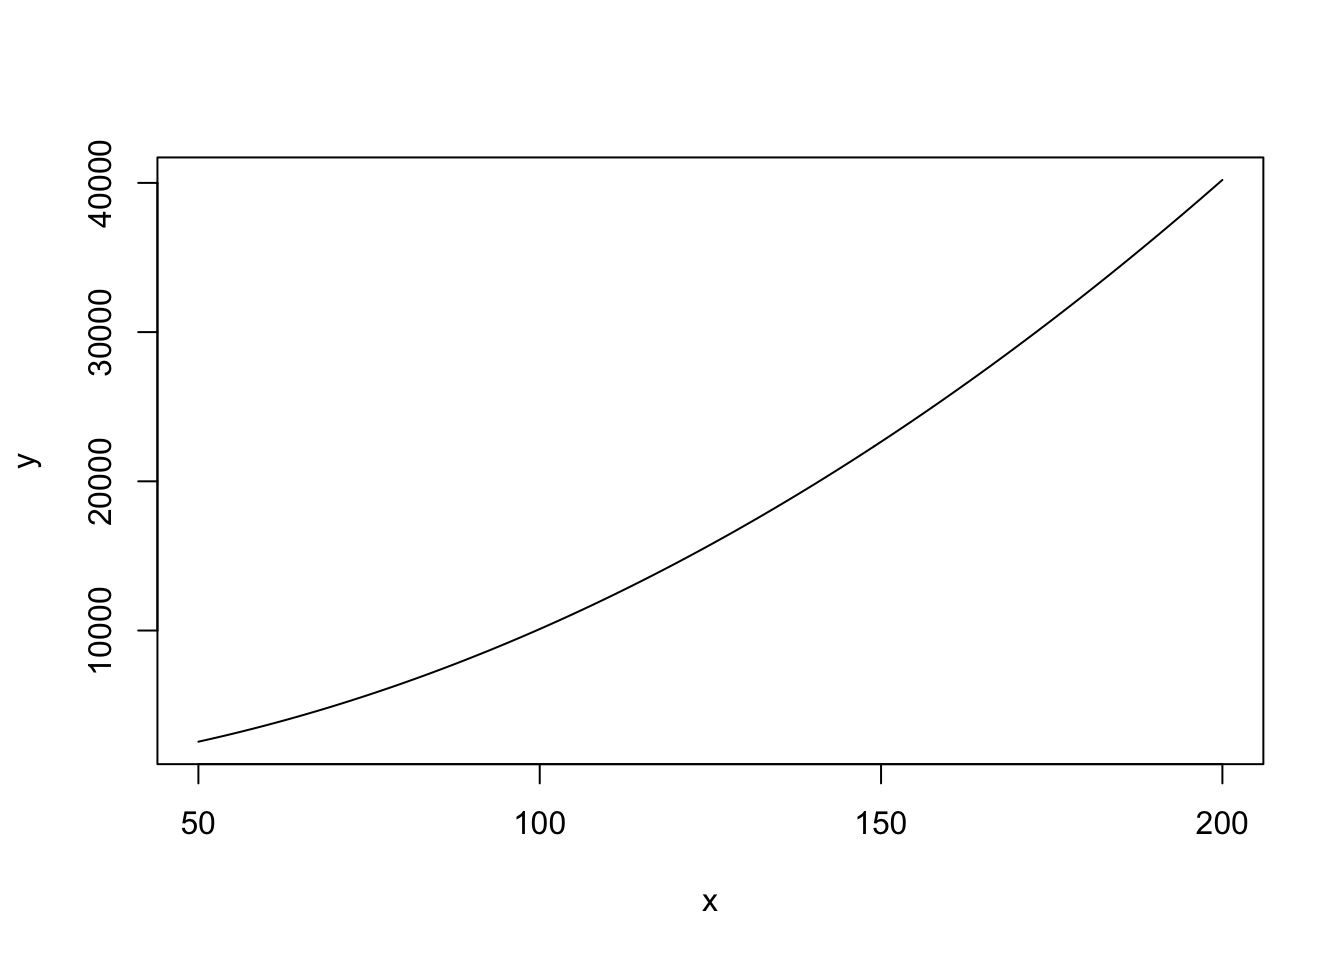
\includegraphics{main_files/figure-latex/unnamed-chunk-150-1.pdf}

Mudeli keeles tähistame me seda, mida me ennustame (antud juhul pikkus)
Y-ga ja seda, mille väärtuse põhjal me ennustame (antud juhul kaal)
X-ga. Seega sirge mudeli matemaatiline formalism on Y = X. See on
äärmiselt jäik mudel: ta on sirge kujuline ja selle sirge asukoht
parameetriruumis on rangelt fikseeritud. Sirge lõikab y telge alati 0-s
(ehk mudeli keeles: selle sirge intercept ehk lõikepunkt Y teljel = 0)
ja tema tõusunurk saab olla ainult 45 kraadi (mudeli keeles: mudeli
slope ehk tõus = 1). Selle mudeli jäikus tuleneb sellest, et selles
mudelis ei ole parameetreid, mida me saaksime vabalt muuta ehk tuunida.

Kuidas aga kirjeldada sirget, mis võib paikneda 2-mõõtmelises ruumis
ükskõik millises asendis? Selleks lisame mudelisse kaks parameetrit,
intercept (a) ja tõus (b). Kui a=0 ja b=0, saame me eelpool kirjeldatud
mudeli y = x. Kui a = 102, siis sirge lõikab y telge väärtusel 102. Kui
b = 0.8, siis x-i tõustes 1 ühiku võrra tõuseb y-i väärtus 0.8 ühiku
võrra. Kui a = 100 ja b = 0, siis saame sirge, mis on paraleelne
x-teljega ja lõikab y telge väärtusel 100 (mis juhtub, kui a = Inf?).
Seega, Teades a ja b väärtusi ning omistades x-le suvalise meid huvitava
väärtuse, saab ennustada y-i keskmist väärtust. Näiteks, olgu andmete
vastu fititud mudel:

pikkus(cm) = 102 + 0.8 * kaal(kg) ehk

y = 102 + 0.8x.

Omistades nüüd kaalule väärtuse 80 kg, tuleb mudeli poolt ennustatud
keskmine pikkus 102 + 0.8 * 80 = 166 cm. Iga kg lisakaalu ennustab
mudeli kohaselt 0.8 cm võrra suuremat pikkust.

\begin{Shaded}
\begin{Highlighting}[]
\NormalTok{a <-}\StringTok{ }\DecValTok{102}
\NormalTok{b <-}\StringTok{ }\FloatTok{0.8}
\NormalTok{x <-}\StringTok{  }\DecValTok{0}\OperatorTok{:}\DecValTok{100} 
\NormalTok{y <-}\StringTok{  }\NormalTok{a }\OperatorTok{+}\StringTok{ }\NormalTok{b }\OperatorTok{*}\StringTok{ }\NormalTok{x}
\KeywordTok{plot}\NormalTok{(y}\OperatorTok{~}\NormalTok{x, }\DataTypeTok{type=}\StringTok{"l"}\NormalTok{, }\DataTypeTok{xlab=}\StringTok{"weight in kg"}\NormalTok{, }\DataTypeTok{ylab=}\StringTok{"heigth in cm"}\NormalTok{, }\DataTypeTok{main=}\StringTok{"a more flexible linear model"}\NormalTok{, }\DataTypeTok{ylim=}\KeywordTok{c}\NormalTok{(}\DecValTok{50}\NormalTok{, }\DecValTok{200}\NormalTok{))}
\end{Highlighting}
\end{Shaded}

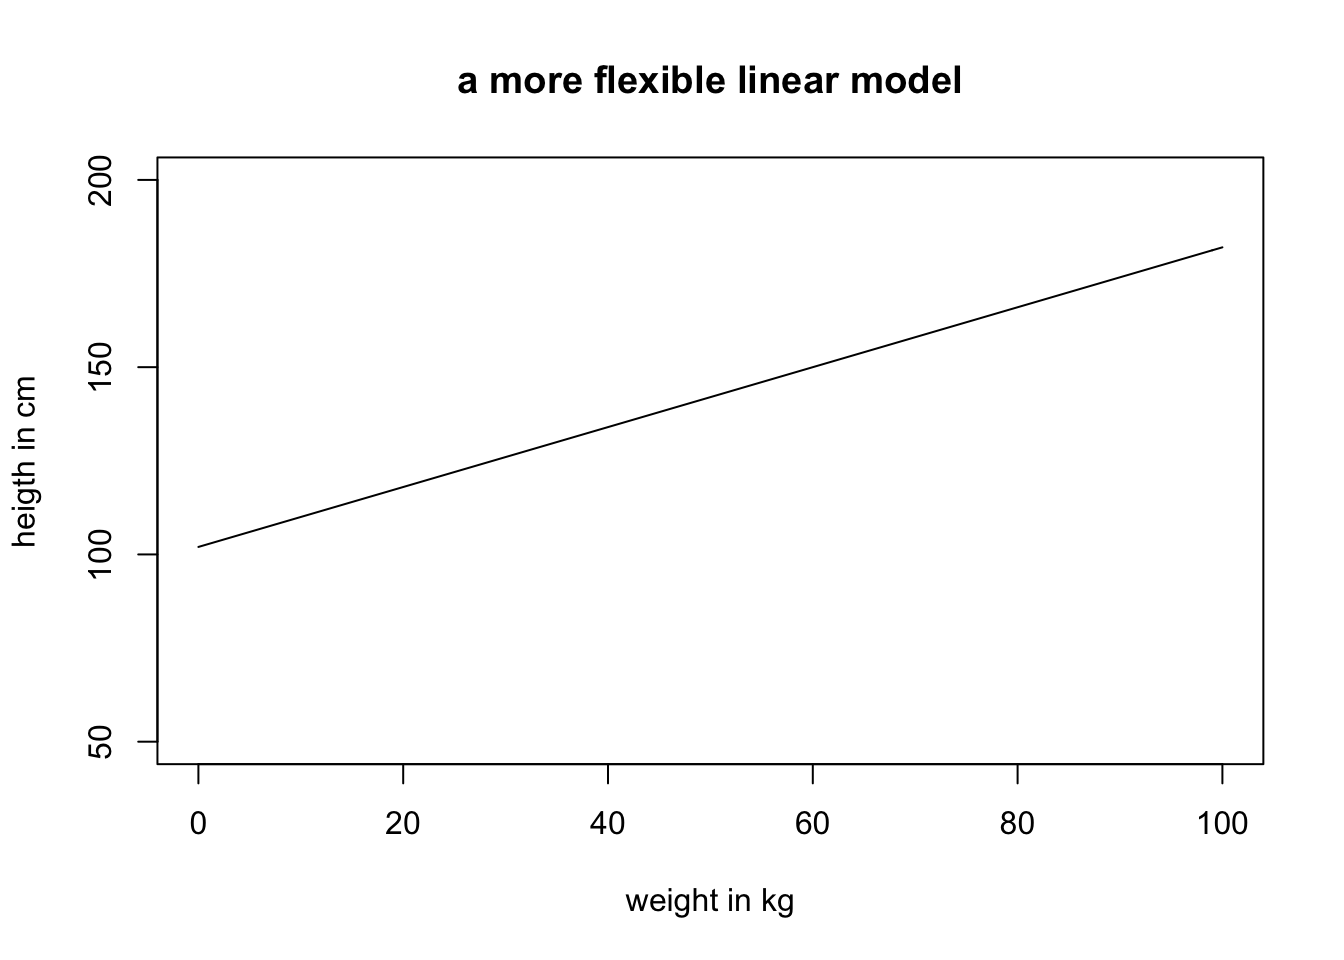
\includegraphics{main_files/figure-latex/unnamed-chunk-151-1.pdf}

See mudel ennustab, et 0 kaalu juures on pikku 102 cm, mis on rumal, aga
mudelite puhul tavaline, olukord. Me tuunime mudelit andmete peal, mis
ei sisalda 0-kaalu (sest 0-kaaluga inimesi pole olemas). Meie
valimiandmed ei peegelda täpselt inimpopulatsiooni. Sirge mudel ei
peegelda täpselt pikkuse-kaalu suhteid vahemikus, kus meil on reaalseid
kaaluandmeid; ja ta teeb seda veelgi vähem seal, kus meil mõõdetud
kaalusid ei ole. Seega pole mõtet imestada, miks mudeli intercept meie
üle irvitab.

\subsection{4 mõistet}\label{moistet}

X ja Y on muutujad, a ja b on parameetrid. Muutujate väärtused
fikseeritakse andmete poolt, parameetrid fititakse muutujate väärtuste
põhjal. Fititud mudel ennustab igale X-i väärtusele vastava kõige
tõenäolisema Y väärtuse (Y keskväärtuse sellel X-i väärtusel).

\begin{quote}
Y - mida me ennustame (dependent variable, predicted varable)
\end{quote}

\begin{quote}
X - mille põhjal me ennustame (independent variable, predictor)
\end{quote}

\begin{quote}
muutuja (variable) - iga asi, mida me valimis mõõdame (X ja Y on kaks
muutujat). Muutuja väärtused on fikseeritud andmete poolt. Muutujal on
sama palju fikseeritud väärtusi kui meil on selle muutuja kohta
mõõtmisandmeid.
\end{quote}

\begin{quote}
parameeter (parameter) - mudeli koefitsient, millele võib omistada
suvalisi väärtusi. Parameetreid tuunides fitime me mudeli võimalikult
hästi sobituma andmetega.
\end{quote}

\subsection{Mudeli fittimine}\label{mudeli-fittimine}

Mudelid sisaldavad (1) matemaatilisi struktuure, mis määravad mudeli
tüübi ning (2) parameetreid, mida saab andmete põhjal tuunida, niiviisi
täpsustades mudeli kuju.

Seda tuunimist nimetatakse mudeli fittimiseks. Mudelit fittides on
eesmärk saavutada antud tüüpi mudeli maksimaalne sobivus andmetega.
Näiteks võrrand y = a + bx määrab mudeli, kus y = x on on see struktuur,
mis tagab, et mudeli tüüp on sirge, ning a ja b on parameetrid, mis
määravad sirge asendi. Seevastu struktuur y = x + x\^{}2 tagab, et
mudeli y = a + b1x + b2x\^{}2 tüüp on parabool, ning parameetrite a, b1
ja b2 väärtused määravad selle parabooli täpse kuju. Ja nii edasi.

Hea mudel on

\begin{enumerate}
\def\labelenumi{(\arabic{enumi})}
\item
  võimalikult lihtsa struktuuriga, mille põhjal on veel võimalik teha
  järeldusi protsessi kohta, mis genereeris mudeli fittimiseks kasutatud
  andmeid;
\item
  sobitub piisavalt hästi andmetega (eriti uute andmetega, mida ei
  kasutatud selle mudeli fittimiseks), et olla relevantne andmeid
  genereeriva protsessi kirjeldus;
\item
  genereerib usutavaid simuleeritud andmeid (see näitab mudeli
  kvaliteeti).
\end{enumerate}

Sageli fititkse samade andmetega mitu erinevat tüüpi mudelit ja püütakse
otsustada, milline neist vastab kõige paremini eeltoodud tingimustele.
Näiteks, kui sirge suudab kaalu järgi pikkust ennustada paremini kui
parabool, siis on sirge mudel kooskõlas teadusliku hüpoteesiga, mis
annaks mehhanismi protsessile, mille käigus kilode lisandumine viiks
laias kaaluvahemikus inimeste pikkuse kasvule ilma, et pikkuse kasvu
tempo kaalu tõustes langeks.

\subsubsection{Üle- ja alafittimine}\label{ule--ja-alafittimine}

Osad mudelite tüübid on vähem paindlikud kui teised (parameetreid
tuunides on neil vähem liikumisruumi). Kuigi sellised mudelid sobituvad
halvemini andmetega, võivad need ikkagi paremini kui mõni paindlikum
mudel välja tuua andmete peidetud olemuse. Mudeldamine eeldab, et me
usume, et meie andmetes leidub nii müra (mida mudel võiks ignoreerida),
kui signaal (mida mudel püüab tabada). Kuna mudeli jaoks näeb müra
samamoodi välja kui signaal, on iga mudel kompromiss üle- ja
alafittimise vahel. Me lihtsalt loodame, et meie mudel on piisavalt
jäik, et mitte liiga palju müra modelleerida ja samas piisavalt
paindlik, et piisaval määral signaali tabada.

Üks kõige jäigemaid mudeleid on sirge, mis tähendab, et sirge mudel on
suure tõenäosusega alafittitud. Keera sirget kuipalju tahad, ikka ei
sobitu ta enamiku andmekogudega. Ja need vähesed andmekogud, mis sirge
mudeliga sobivad, on genereeritud teatud tüüpi lineaarsete protsesside
poolt. Sirge on seega üks kõige paremini tõlgendatavaid mudeleid. Teises
äärmuses on polünoomsed mudelid, mis on väga paindlikud, mida on väga
raske tõlgendada ja mille puhul on suur mudeli ülefittimise oht.
Ülefititud mudel järgib nii täpselt valimiandmeid, et sobitub hästi
valimis leiduva juhusliku müraga ning seetõttu sobitub halvasti järgmise
valimiga samast populatsioonist (sest igal valimil on oma juhuslik
müra). Üldiselt, mida rohkem on mudelis tuunitavaid parameetreid, seda
paindlikum mudel, seda kergem on seda valimiandmetega sobitada ja seda
raskem on seda mudelit tõlgendada. Veelgi enam, alati on võimalik
konstrueerida mudel, mis sobitub täiuslikult lõpliku arvu
andmepunktidega (selle mudeli parameetrite arv = N). Selline mudel on
täpselt sama informatiivne kui andmed, mille põhjal see fititi --- ja
täiesti kasutu.

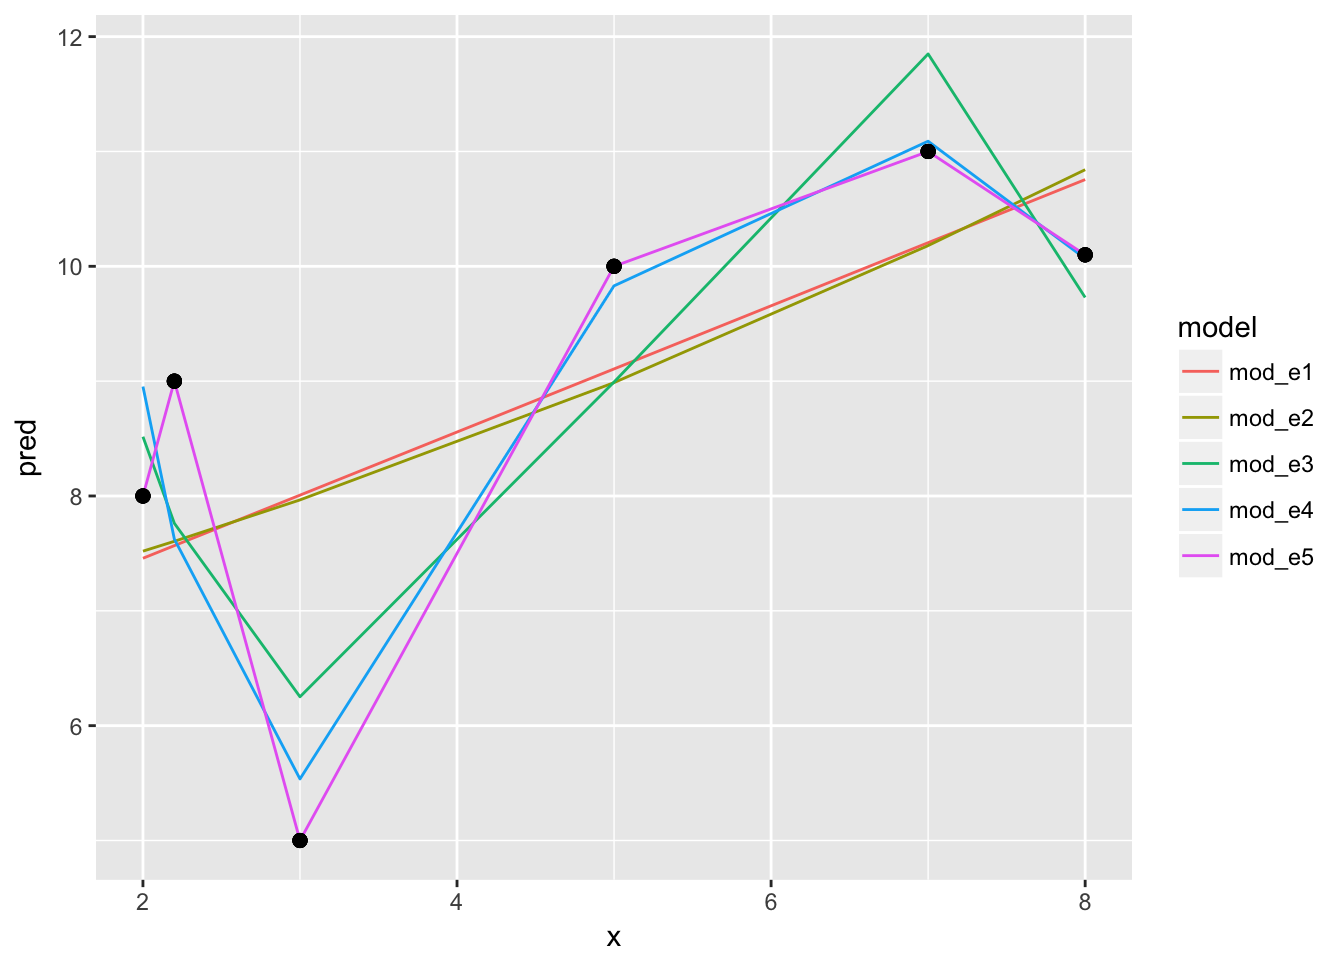
\includegraphics{main_files/figure-latex/unnamed-chunk-152-1.pdf}
\emph{Joonis: Kasvava paindlikusega polünoomsed mudelid. mod\_e1 on
sirge võrrand y = a + b1x (2 parameetrit: a ja b1), mod\_e2 on lihtsaim
võimalik polünoom: y= a + b1x + b2x\^{}2 (3 parameetrit), \ldots{},
mod\_e5: y= a + b1x + b2x\^{}2 + b3x\^{}3 + b4x\^{}4 + b5x\^{}5 (6
parameetrit). mod\_e5 vastab täpselt andmepunktidele (N = 6).}

\begin{Shaded}
\begin{Highlighting}[]
\KeywordTok{AIC}\NormalTok{(mod_e1, mod_e2, mod_e3, mod_e4, mod_e5)}
\end{Highlighting}
\end{Shaded}

\begin{verbatim}
##        df      AIC
## mod_e1  3 27.77993
## mod_e2  4 29.76669
## mod_e3  5 26.21330
## mod_e4  6 25.11245
## mod_e5  7     -Inf
\end{verbatim}

AIC näitab, et parim mudel on mod\_e4. Aga kas see on ka kõige kasulikum
mudel? Mis siis, kui 3-s andmepunkt on andmesisestaja näpuviga?

\begin{verbatim}
AIC - Akaike Informatsiooni Kriteerium - vaatab mudeli sobivust andmetega
ja mudeli parameetrite arvu. 
Väikseim AIC tähitab parimat fitti väikseima parameetrite arvu juures
(kompromissi) ja väikseima AIC-ga mudel on eelistatuim mudel. Aga seda ainult
võrreldud mudelite hulgas. AIC-i absoluutväärtus ei loe - see on suhteline näitaja.  
\end{verbatim}

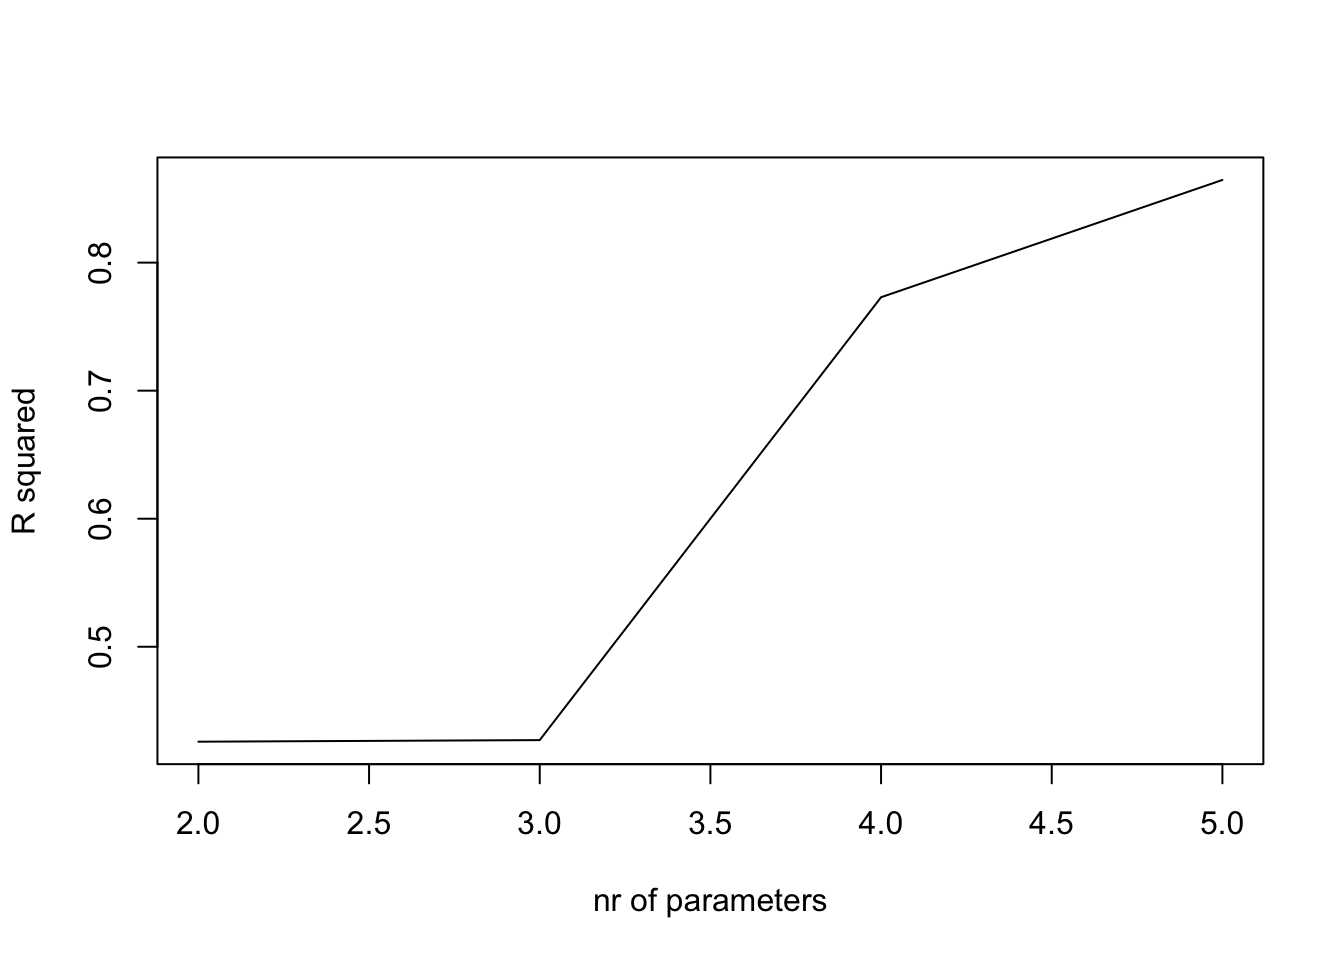
\includegraphics{main_files/figure-latex/unnamed-chunk-154-1.pdf}
\emph{Joonis: sedamööda kuidas parameetrite arv mudelis kasvab, kasvab
ka R ruut. R ruut 0.8 tähendab, et x-i varieeruvus suudab seletada kuni
80\% y-i varieeruvusest. Lisaparameetri lisamine ei saa põhimõtteliselt
R ruutu vähendada. Aga selle kasvu kiirus on aeglustuv. Ühel hetkel ei
õigusta mudeli fiti paranemine enam mudeli paindlikuse kasvu (mis
mõlemad saavutatakse parameetreid lisades).}

\begin{verbatim}
Ülefittimise vältimiseks kasutavad Bayesi mudelid informatiivseid prioreid, 
mis välistavad ekstreemsed parameetriväärtused. 
Vt http://elevanth.org/blog/2017/08/22/there-is-always-prior-information/ 
\end{verbatim}

\subsection{Veamudel}\label{veamudel}

Eelpool kirjeldatud mudelid on deterministlikud --- nad ei sisalda
hinnangut andmete varieeruvusele ennustuse ümber. Neid kutsutakse ka
\textbf{protsessi mudeliteks} sest nad modelleerivad protsessi täpselt.
Ehk kui mudel ennustab, et 80 kg inimene on 166 cm pikkune, siis
protsessi mudel ei ütle, kui suurt kaalust sõltumatut pikkuste
varieeruvust võime oodata 80 kg-ste inimeste hulgas? Selle hinnangu
andmiseks tuleb mudelile lisada veel üks komponent, \textbf{veamudel}
ehk veakomponent, mis sageli tuuakse sisse normaaljaotuse kujul.
Veakomponent modelleerib üksikute inimeste pikkuste varieeruvust (mitte
keskmise pikkuse varieeruvust) igal mõeldaval ja mittemõeldaval kaalul.
Tänu sellele ei ole mudeli ennustused enam deterministlikud, vaid
tõenäosuslikud.

Kuidas veakomponent lineaarsesse mudelisse sisse tuua?

ilma veakomponendita mudel: \emph{y = a + bx}

Veakomponent tähendab, et y-i väärtus varieerub ümber mudeli poolt
ennustatud keskväärtuse ja seda varieeruvust normaaljaotusega
modelleerides saame

\emph{y \textasciitilde{} dnorm(mu, sigma)}

kus \emph{mu} on mudeli poolt ennustatud keskväärtus ja \emph{sigma} on
mudeli poolt ennustatud standardhälve ehk varieeruvus andmepunktide
tasemel. Tilde \textasciitilde{} tähistab seose tõenäosuslikkust.

Sirge mudelisse varieeruvuse sisse toomiseks defineerime mu ümber nõnda:

\emph{mu = a + bx}, mis tähendab, et

\emph{y \textasciitilde{} dnorm(a + bx, sigma)}

See ongi sirge mudel koos veakomponendiga. Peatükis 3 õpime me selliste
mudelitega töötama.

\begin{quote}
Kõik statistilised mudelid on tõenäosusmudelid ning sisaldavad
veakomponenti.
\end{quote}

\subsection{Statistiline mudel koosneb 3
komponendist:}\label{statistiline-mudel-koosneb-3-komponendist}

\begin{verbatim}
> (1) matemaatiline struktuur, mis sisaldab muutujaid ja annab mudeli tüübi, 

> (2) tuunitavad parameetrid ja 

> (3) veamudel.
\end{verbatim}

Muide, kõik veamudelid, millega me edaspidi töötame, modelleerivad igale
x-i väärtusele (kaalule) sama suure y-i suunalise varieeruvuse (pikkuste
sd). Suurem osa statistikast kasutab eeldusi, mida keegi päriselt tõe
pähe ei võta, aga millega on arvutuslikus mõttes lihtsam elada.

\subsubsection{Enimkasutatud veamudel on
normaaljaotus.}\label{enimkasutatud-veamudel-on-normaaljaotus.}

Oletame, et meil on kolm andmepunkti ning me usume, et need andmed on
juhuslikult tõmmatud normaaljaotusest või sellele lähedasest jaotusest.
Normaaljaotuse mudelit kasutades me sisuliselt deklareerime, et me
usume, et kui me oleksime olnud vähem laisad ja 3 mõõtmise asemel
sooritanuks 3000, siis need mõõtmised sobituksid piisavalt hästi meie 3
väärtuse peal fititud normaaljaotusega. Seega, me usume, et omades 3
andmepunkti me teame juba umbkaudu, millised tulemused me oleksime
saanud korjates näiteks 3 miljonit andmepunkti. Oma mudelist võime
simuleerida ükskõik kui palju andmepunkte.

Aga pidage meeles, et selle mudeli fittimiseks kasutame me ainult neid
andmeid, mis meil päriselt on --- ja kui meil on ainult 3 andmepunkti,
on tõenäoline, et fititud mudel ei kajasta hästi tegelikkust.

\begin{quote}
Halvad andmed ei anna kunagi head tulemust.
\end{quote}

Eelnev ei kehti Bayesi mudelite kohta, mis toovad priorite kaudu sisse
lisainfot, mis ei kajastu valimiandmetes ja võib analüüsi päästa.

Kuidas panna skeptik uskuma, et statistilised meetodid töötavad halvasti
väikestel valimitel? Siin aitab simulatsioon, kus me tõmbame 3-se valimi
etteantud populatsioonist ning üritame selle valimi põhjal ennustada
selleasama populatsiooni struktuuri. Kuna tegemist on simulatsiooniga,
teame täpselt, et populatsioon, kust me tõmbame oma kolmese valimi, on
normaaljaotusega, et tema keskväärtus = 0 ja et tema sd = 1. Me fitime
oma valimi andmetega 2 erinevat mudelit: normaaljaotuse ja Studenti t
jaotuse.

\begin{verbatim}
## `stat_bindot()` using `bins = 30`. Pick better value with `binwidth`.
\end{verbatim}

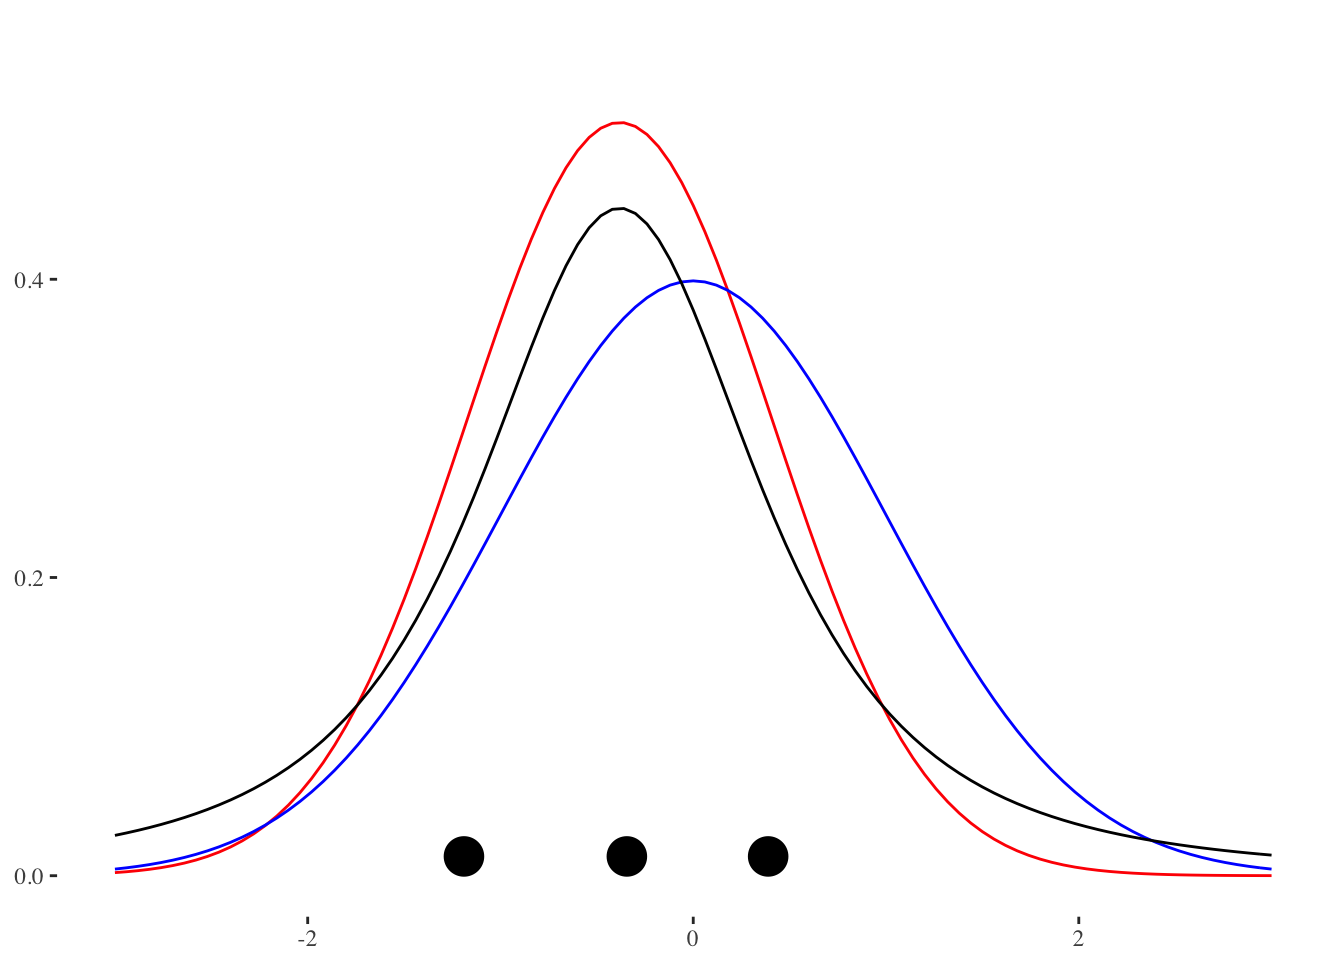
\includegraphics{main_files/figure-latex/unnamed-chunk-155-1.pdf}

\emph{Joonis: juhuvalim normaaljaotusest, mille keskmine=0 ja sd=1 (n=3;
andmepunktid on näidatud mustade munadena). Sinine joon - popualtsioon,
millest tõmmati valim; punane joon - normaaljaotuse mudel, mis on
fititud valimi andmetel; must joon - Studenti t jaotuse mudel, mis on
fititud samade andmetega.}

Mõlemad mudelid on süstemaatiliselt nihutatud väiksemate väärtuste poole
ja alahindavad varieeruvust. t jaotuse mudel on oodatult paksemate
sabadega ja ennustab 0-st kaugele palju rohkem väärtusi kui
normaaljaotuse mudel. Kuna me teame, et populatsioon on
normaaljaotusega, pole väga üllatav, et t jaotus modeleerib seda
halvemini kui normaaljaotus.

Igal juhul, mõni teine juhuvalim annaks meile hoopis teistsugused
mudelid, mis rohkem või vähem erinevad algsest populatsioonist.

Mis juhtub kui me kasutame oma normaaljaotuse mudelit uute andmete
simuleerimiseks? Kui lähedased on need simuleeritud andmed populatsiooni
andmetega ja kui lähedased valimi andmetega, millega me normaaljaotuse
mudeli fittisime?

\begin{Shaded}
\begin{Highlighting}[]
\KeywordTok{set.seed}\NormalTok{(}\DecValTok{19}\NormalTok{) }\CommentTok{#muudab simulatsiooni korratavaks}
\CommentTok{#tõmbame 3 juhuslikku arvu normaalhaotusest, mille keskväärtus = 0 ja sd = 1.}
\NormalTok{df <-}\StringTok{ }\KeywordTok{tibble}\NormalTok{(}\DataTypeTok{sample_data=}\KeywordTok{rnorm}\NormalTok{(}\DecValTok{3}\NormalTok{)) }
\CommentTok{#fitime normaaljaotuse mudeli valimi keskmise ja sd-ga}
\KeywordTok{mean}\NormalTok{(df}\OperatorTok{$}\NormalTok{sample_data); }\KeywordTok{sd}\NormalTok{(df}\OperatorTok{$}\NormalTok{sample_data)}
\end{Highlighting}
\end{Shaded}

\begin{verbatim}
## [1] -0.3817353
\end{verbatim}

\begin{verbatim}
## [1] 0.7896821
\end{verbatim}

\begin{Shaded}
\begin{Highlighting}[]
\CommentTok{#simuleerime 1000 uut andmepunkti fititud mudelist}
\NormalTok{simulated_data <-}\StringTok{ }\KeywordTok{rnorm}\NormalTok{(}\DecValTok{1000}\NormalTok{, }\KeywordTok{mean}\NormalTok{(df}\OperatorTok{$}\NormalTok{sample_data), }\KeywordTok{sd}\NormalTok{(df}\OperatorTok{$}\NormalTok{sample_data))}
\CommentTok{#arvutame simuleeritud andmete keskmise ja sd ning joonistame neist histogrammi}
\KeywordTok{mean}\NormalTok{(simulated_data); }\KeywordTok{sd}\NormalTok{(simulated_data); }\KeywordTok{hist}\NormalTok{(simulated_data)}
\end{Highlighting}
\end{Shaded}

\begin{verbatim}
## [1] -0.3848133
\end{verbatim}

\begin{verbatim}
## [1] 0.7749198
\end{verbatim}

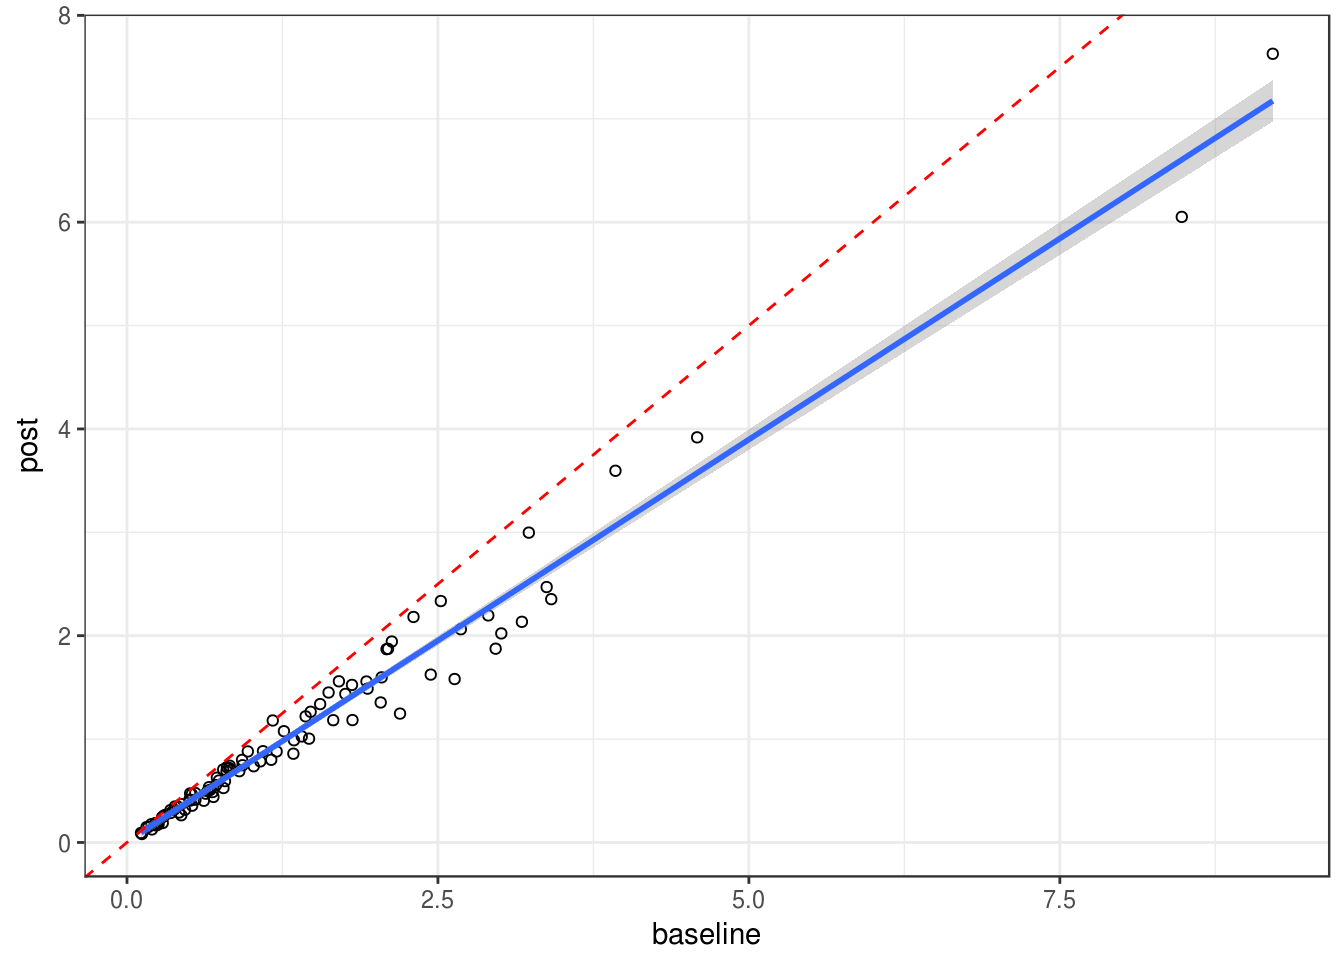
\includegraphics{main_files/figure-latex/unnamed-chunk-156-1.pdf}

Nagu näha, on uute (simuleeritud) andmete keskväärtus ja SD väga
sarnased algsete andmete omale, mida kasutasime mudeli fittimisel.
Kahjuks ei ole need aga kaugeltki nii sarnased algsele jaotusele, mille
kuju me püüame oma andmete ja mudeli pealt ennustada. Seega on meie
mudel üle-fittitud, mis tähendab, et ta kajastab liigselt neid valimi
aspekte, mis ei peegelda algse populatsiooni omadusi. Loomulikult ei
vasta ükski mudel päriselt tegelikkusele. Küsimus on pigem selles, kas
mõni meie mudelitest on piisavalt hea, et olla kasulik. Vastus sellele
sõltub, milleks plaanime oma mudelit kasutada.

\begin{Shaded}
\begin{Highlighting}[]
\KeywordTok{mean}\NormalTok{(simulated_data}\OperatorTok{>}\DecValTok{0}\NormalTok{); }\KeywordTok{mean}\NormalTok{(simulated_data}\OperatorTok{>}\DecValTok{1}\NormalTok{)}
\end{Highlighting}
\end{Shaded}

\begin{verbatim}
## [1] 0.317
\end{verbatim}

\begin{verbatim}
## [1] 0.037
\end{verbatim}

Kui populatsiooniväärtustest on 50\% suuremad kui 0, siis mudeli järgi
vaevalt 32\%. Kui populatsiooniväärtustest on 16\% suuremad kui 1, siis
mudeli järgi vaevalt 4\%. See illustreerib hästi mudeli kvaliteeti.

\begin{Shaded}
\begin{Highlighting}[]
\KeywordTok{library}\NormalTok{(brms)}
\NormalTok{sim_t <-}\StringTok{ }\KeywordTok{rstudent_t}\NormalTok{(}\DecValTok{1000}\NormalTok{, }\DecValTok{2}\NormalTok{, }\KeywordTok{mean}\NormalTok{(df}\OperatorTok{$}\NormalTok{sample_data), }\KeywordTok{sd}\NormalTok{(df}\OperatorTok{$}\NormalTok{sample_data))}
\KeywordTok{mean}\NormalTok{(sim_t}\OperatorTok{>}\DecValTok{0}\NormalTok{); }\KeywordTok{mean}\NormalTok{(sim_t}\OperatorTok{>}\DecValTok{1}\NormalTok{)}
\end{Highlighting}
\end{Shaded}

\begin{verbatim}
## [1] 0.338
\end{verbatim}

\begin{verbatim}
## [1] 0.11
\end{verbatim}

Samad ennustused t jaotusest on isegi paremad! Aga kumb on ikkagi parem
mudel populatsioonile?

\subsection{normaaljaotuse ja lognormaaljaotuse
erilisus}\label{normaaljaotuse-ja-lognormaaljaotuse-erilisus}

Normaaljaotus ja lognormaaljaotus on erilised sest

\begin{enumerate}
\def\labelenumi{(\arabic{enumi})}
\item
  keskne piirteoreem ütleb, et olgu teie valim ükskõik millise
  jaotusega, paljudest valimitest arvutatud \textbf{aritmeetilised
  keskmised} on alati enam-vähem normaaljaotusega (kui
  n\textgreater{}30). Selle matemaatilise formalismi tuletus
  füüsikalisse maailma on nn ``elementaarsete vigade hüpotees'', mille
  kohaselt paljude väikeste üksteisest sõltumatute juhuslike efektide
  (vigade) summa annab tulemuseks normaaljaotuse. Paraku annavad enamus
  bioloogilisi mõõtmisi eranditult mitte-negatiivseid tulemusi. Sageli
  on selliste mõõtmiste tulemuste jaotused ebasümmeetrilised (v.a. siis,
  kui cv = sd/mean on väike) ja siis on meil sageli tegu
  lognormaaljaotusega, mis tekkib log-normaalsete muutujate
  korrutamisest (mitte liitmisest, nagu normaaljaotuse puhul). Keskne
  piirteoreem 2: suvalise jaotusega muutujate \textbf{geomeetrilised
  keskmised} on lognormaaljaotusega. Elementaarsete vigade hüpotees 2:
  Kui juhuslik varieeruvus tekib paljude juhuslike efektide
  korrutamisel, on tulemuseks lognormaaljaotus. Lognormaaljaotuse
  elementide (arvude) logaritmimisel saame normaaljaotuse.
\item
  Mõlemad jaotused (normaal ja lognormaal) on maksimaalse entroopiaga
  jaotused. Entroopiat vaadeldakse siin informatsiooni/müra kaudu ---
  maksimaalse entroopiaga süsteem sisaldab maksimaalselt müra ja
  minimaalselt informatsiooni (Shannoni informatsiooniteooria). See
  tähendab, et väljaspool oma parameetrite tuunitud väärtusi on need
  normaal- ja lognormaaljaotused minimaalselt informatiivsed. Näiteks
  normaaljaotusel on kaks parameetrit, mu ja sigma (ehk keskmine ja
  standardhälve). Seega, andes normaaljaotusele ette keskväärtuse ja
  standardhälbe fikseerime üheselt jaotuse ehk mudeli kuju ja samas
  lisame sinna minimaalselt muud (sooviamtut) informatsiooni. Teised
  maksimaalse entroopiaga jaotused on eksponentsiaalne jaotus,
  binoomjaotus ja poissoni jaotus. Maksimaalse entroopiaga jaotused
  sobivad hästi Bayesi prioriteks sest me suudame paremini kontrollida,
  millist informatsiooni me neisse surume.
\end{enumerate}

\section{Küsimused, mida statistika
küsib}\label{kusimused-mida-statistika-kusib}

Statistika abil saab vastuseid järgmisetele küsimustele:

\begin{enumerate}
\def\labelenumi{\arabic{enumi})}
\item
  kuidas näevad välja teie andmed ehk milline on just teie andmete
  jaotus, keskväärtus, varieeruvus ja koos-varieeruvus? Näiteks,
  mõõdetud pikkuste ja kaalude koos-varieeruvust saab mõõta
  korrelatsioonikordaja abil.
\item
  mida me peaksime teie valimi andmete põhjal uskuma populatsiooni
  parameetri tegeliku väärtuse kohta? Näiteks, kui meie andmete põhjal
  arvutatud keskmine pikkus on 178 cm, siis kui palju on meil põhjust
  arvata, et tegelik populatsiooni keskmine pikkus \textgreater{} 185
  cm?
\item
  mida ütleb statistilise mudeli struktuur teadusliku hüpoteesi kohta?
  Näiteks, kui meie poolt mõõdetud pikkuste ja kaalude koos-varieeruvust
  saab hästi kirjeldada kindlat tüüpi lineaarse regressioonimudeliga,
  siis on meil ehk tõendusmaterjali, et pikkus ja kaal on omavahel
  sellisel viisil seotud ja eelistatud peaks olema teaduslik teooria,
  mis just sellise seose tekkimisele bioloogilise mehhanismi annab.
\item
  mida ennustab mudel tuleviku kohta? Näiteks, meie lineaarne
  pikkuse-kaalu mudel suudab ennustada tulevikus kogutavaid pikkuse
  andmeid. Aga kui hästi?
\end{enumerate}

\begin{quote}
statistika ülesanne on lähtuvalt piiratud hulgast andmetest ja
mudelitest kvantifitseerida parimal võimalikul viisil kõhedust, mida
peaksime tundma vastates eeltoodud küsimustele.
\end{quote}

Statistika ei vasta otse teaduslikele küsimustele ega küsimustele päris
maailma kohta. Statistilised vastused jäävad alati kasutatud andmete ja
mudelite piiridesse. Sellega seoses peaksime eelistama hästi kogutud
rikkalikke andmeid ja paindlikke mudeleid. Siis on lootust, et hüpe
mudeli koefitsientidest päris maailma kirjeldamisse tuleb üle kitsama
kuristiku. Bayesil on siin eelis, sest osav statistik suudab koostöös
teadlastega priori mudelisse küllalt palju kasulikku infot koguda.
Samas, amatöör suudab bayesi abil samavõrra käkki keerata. Mida
paindlikum on meetod, seda vähem automaatne on selle mõistlik
kasutamine.

\chapter{2 osa. Kuidas näevad välja teie
andmed?}\label{osa.-kuidas-naevad-valja-teie-andmed}

\section{summaarsed statistikud}\label{summaarsed-statistikud}

Summaarne statistik = üks number.\\
Milliseid statistikuid arvutada ja milliseid vältida, sõltub
statistilisest mudelist

\begin{quote}
summaarse statistika abil iseloomustame a) tüüpilist valimi liiget
(keskmist), b) muutuja sisest varieeruvust, c) erinevate muutujate
(pikkus, kaal vms) koos-varieeruvust
\end{quote}

\subsection{keskväärtused}\label{keskvaartused}

Keskväärtust saab mõõta paaril tosinal erineval viisil, millest
järgnevalt kasutame kolme või nelja. Enne kui te arvutama kukute, mõelge
järele, miks te soovite keskväärtust teada. Kas teid huvitab valimi
tüüpiline liige? Kuidas te sooviksite seda tüüpilisust defineerida? Kas
valimi keskmise liikmena või valimi kõige arvukama liikmena? või veel
kuidagi? See, millist keskväärtust kasutada sõltub sageli andmejaotuse
kujust. Sümmeetrilisi jaotusi on lihtsam iseloomustada ja mitmetipulised
jaotused on selles osas kõige kehvemad.

Mina eelistan selliseid nõuandeid (mis on rangelt soovituslikud):

\begin{enumerate}
\def\labelenumi{(\arabic{enumi})}
\item
  Kui valim on normaaljaotusega (histogramm on sümmeetriline), hinda
  tüüpilist liiget läbi aritmeetilise keskmise (mean).
\item
  Muidu kasuta mediaani (median). Kui valim on liiga väike, et jaotust
  hinnata (aga \textgreater{} 4), eelista mediaani. Mediaani saamiseks
  järjestatakse mõõdetud väärtused suuruse järgi ja võetakse selle rea
  keskmine liige. Mediaan on vähem tundlik ekstreemsete väärtuste
  (outlierite) suhtes kui mean.
\item
  Valimi kõige levinumat esindajat iseloomustab mood ehk jaotuse tipp.
  Seda on aga raskem täpselt määrata ja mitmetipulisel jaotusel on mitu
  moodi. Töötamisel posterioorsete jaotustega on mood sageli parim
  lahendus.
\end{enumerate}

\begin{verbatim}
## [1] 0.6817168
\end{verbatim}

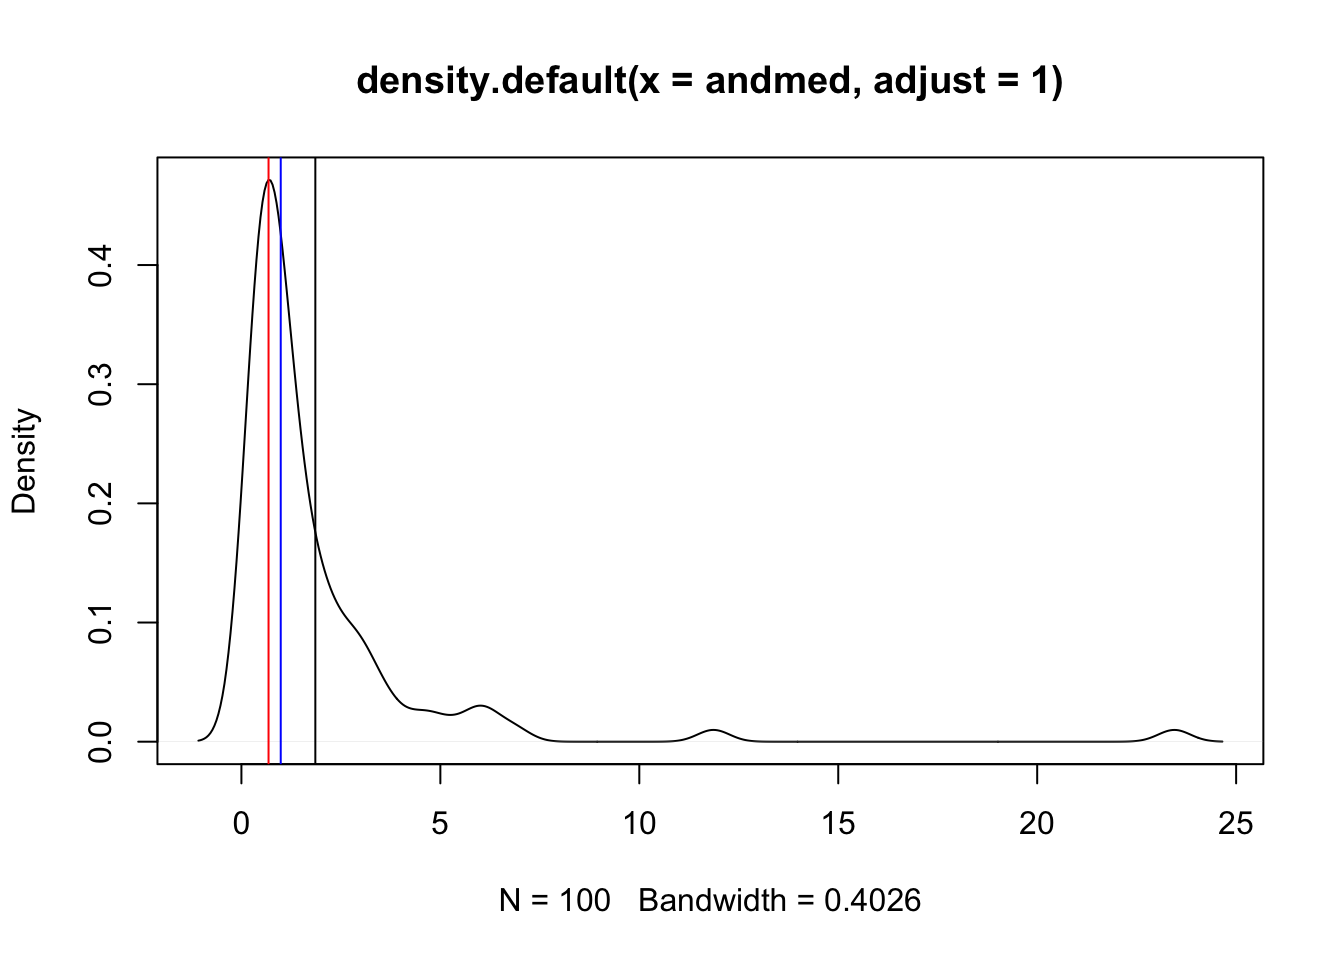
\includegraphics{main_files/figure-latex/unnamed-chunk-159-1.pdf}
Joonis: Simuleeritud lognormaaljaotusega andmed. Punane joon - mood;
sinine joon - mediaan; must joon - aritmeetiline keskmine (mean).
Milline neist vastab parimini teie intuitsiooniga nende andmete
``keskväärtusest''? Miks?

\subsection{muutuja sisene
varieeruvus}\label{muutuja-sisene-varieeruvus}

Mean-iga käib kokku standardhälve (SD).

SD on sama ühikuga, mis andmed (ja andmete keskväärtus). Statistikute
hulgas eelistatud formaat on mean (SD), mitte mean (+/- SD). 1 SD katab
68\% normaaljaotusest, 2 SD -- 96\% ja 3 SD -- 99\%. Normaaljaotus
langeb servades kiiresti, mis tähendab, et tal on peenikesed sabad ja
näiteks 5 SD kaugusel keskmisest paikneb vaid üks punkt miljonist.

Näiteks: inimeste IQ on normaaljaotusega, mean=100, sd=15. See tähendab,
et kui sinu IQ=115 (ülikooli astujate keskmine IQ), siis on tõenäosus,
et juhuslikult kohatud inimene on sinust nutikam, 18\% ((100\% - 68\%)/2
= 18\%).

Kui aga ``tegelikul'' andmejaotusel on ``paks saba'' või esinevad
outlierid, siis normaaljaotust eeldav mudel tagab ülehinnatud SD ja
seega ülehinnatud varieeruvuse. Kui andmed saavad olla ainult
positiivsed, siis SD \textgreater{} mean/2 viitab, et andmed ei sobi
normaaljaotuse mudeliga (sest mudel ennustab negatiivsete andmete
esinemist küllalt suure sagedusega).

\begin{verbatim}
Normaaljaotus on defineeritud ka mõnede teiste jaotuste jaoks peale normaaljaotuse 
(Poissioni jaotus, binoomjaotus). 
Funktsioon sd() ja selle taga olev valem, mis on loodud normaaljaotuse tarbeks, 
ja neid alternatiivseid standardhälbeid ei arvuta. 
Seega tasub meeles pidada, et tavapärane sd kehtib normaaljaotuse mudeli piirides ja ei kusagil mujal!
\end{verbatim}

Kui andmed ei sobi normaaljaotusesse siis võib pakkuda kahte
alternatiivset lahendust:

\subsubsection{(1) logaritmi andmed.}\label{logaritmi-andmed.}

Kui logaritmimine muudab andmed normaalseks, siis saab logaritmitud
andmetest arvutada mean-i ja SD ja seejärel mõlemad anti-logaritmida.
Sellisel juhul avaldad sa lõpuks geomeetrilise keskmise ja
multiplikatiivse SD (multiplikatiivne SD = geom mean x SD; geom
mean/SD). Geomeetriline keskmine on alati väiksem kui aritmeetiline
keskmine. Lisaks on SD interval nüüd asümmeetriline ja SD on alati
\textgreater{} 0. Nagu ennegi, 68\% lognormaalsetest andmetest jääb 1SD
vahemikku ning 95.5\% andmetest jääb 2SD vahemikku.

lognormaalsete andmete tavapärane iseloomustus keskmise ja
standardhälbega: mean(sd) on 1.8(1.9). See sd interval on sümmeetriline,
ehkki andmete jaotus on vägagi ebasümmeetriline. Lisaks ennustab
standardhälve, mis on suurem kui keskväärtus, suure sagedusega
negatiivseid väärtusi. Sageli on aga negatiivsed muutuja väärtused
võimatud (näiteks nädalas suitsetatud sigarettide arv). See on näide
halvast mudelist!

Juhul kui tegu lognormaalsete andmetega on meil võimalus kasutada palju
paremat mudelit varieeruvusele - multiplikatiivset standardhälvet:

\begin{verbatim}
## # A tibble: 4 x 4
##                   SD     MEAN      lower    upper
##                <chr>    <dbl>      <dbl>    <dbl>
## 1  multiplicative_SD 1.084891  0.4010893 2.934481
## 2 multiplicative_2SD 1.084891  0.1482845 7.937367
## 3        additive_SD 1.857924 -0.9636351 4.679482
## 4       additive_2SD 1.857924 -3.7851938 7.501041
\end{verbatim}

Tavalise aritmeetitilise keskmise asemel on meil nüüd geomeetriline
keskmine. Võrdluseks on antud ka tavaline (aritmeetiline) keskmine ja
(aditiivne) SD. Additiivne SD on selle jaotuse kirjeldamiseks selgelt
ebaadekvaatne (vt jaotuse pilti ülalpool ja võrdle mulitplikatiivse
SD-ga).

Kuidas aga töötab multiplikatiivne standardhälve normaaljaotusest pärit
andmetega? Kui normaalsete andmete peal multiplikatiivse sd rakendamine
viib katastroofini, siis pole sel statistikul suurt praktilist
kasutusruumi.

\begin{Shaded}
\begin{Highlighting}[]
\KeywordTok{set.seed}\NormalTok{(}\DecValTok{5363}\NormalTok{)}
\NormalTok{norm_andmed <-}\StringTok{ }\KeywordTok{rnorm}\NormalTok{(}\DecValTok{3}\NormalTok{, }\DecValTok{100}\NormalTok{, }\DecValTok{20}\NormalTok{)}
\KeywordTok{multiplicative_sd}\NormalTok{(norm_andmed)}
\end{Highlighting}
\end{Shaded}

\begin{verbatim}
## # A tibble: 4 x 4
##                   SD     MEAN    lower    upper
##                <chr>    <dbl>    <dbl>    <dbl>
## 1  multiplicative_SD 108.1088 92.80205 125.9403
## 2 multiplicative_2SD 108.1088 79.66252 146.7128
## 3        additive_SD 108.9603 92.08395 125.8367
## 4       additive_2SD 108.9603 75.20756 142.7131
\end{verbatim}

Nagu näha, on multiplikatiivse sd kasutamine normaalsete andmetega üsna
ohutu (kuigi, ainult niikaua, kuni meil puuduvad negatiivsed andmed).
Seega, kui sa ei ole kindel, kas tegu on normaaljaotusega või
lognormaaljaotusega, arvesta, et lognormaaljaotus on bioloogias üsna
tavaline (eriti ensüümreaktsioonide ja kasvuprotsesside juures). Seega
on mõistlik alati kasutada multiplicative\_sd() funktsiooni ja kui
mõlema SD väärtused on sarnased, siis võib loota, et andmed on
normaalsed ning saab avaldada tavapärase additiivse SD refereede
rõõmuks.

\begin{quote}
kui n \textless{} 10, siis mõlemad SD-d alahindavad tehnilistel
põhjustel tegelikku sd-d. Ettevaatust väikeste valimitega!
\end{quote}

\subsubsection{(2) iseloomusta andmeid algses skaalas: median
(MAD).}\label{iseloomusta-andmeid-algses-skaalas-median-mad.}

MAD ---- median absolute deviation --- on vähem tundlik outlierite
suhtes ja ei eelda normaaljaotust. Puuduseks on, et MAD ei oma
tõlgendust, mille kohaselt ta hõlmaks kindlat protsenti populatsiooni
või valimi andmejaotusest. Seevastu sd puhul võime olla kindlad, et
isegi kõige hullema jaotuse korral jäävad vähemalt 75\% andmetest 2 SD
piiridesse.

\begin{Shaded}
\begin{Highlighting}[]
\KeywordTok{mad}\NormalTok{(andmed, }\DataTypeTok{constant =} \DecValTok{1}\NormalTok{)}
\end{Highlighting}
\end{Shaded}

\begin{verbatim}
## [1] 0.5950562
\end{verbatim}

\begin{verbatim}
 Ära kunagi avalda andmeid vormis: mean (MAD) või median (SD). 
 Korrektne vorm on mean(SD) või median(MAD).
\end{verbatim}

\subsection{muutujate
koos-varieeruvus}\label{muutujate-koos-varieeruvus}

Andmete koos-varieeruvust mõõdetakse korrelatsiooni abil. Tulemuseks on
üks number - korrelatsioonikordaja r, mis varieerub -1 ja 1 vahel.

\begin{verbatim}
r = 0 – kahte tüüpi mõõtmised (x=pikkus, y=kaal) samadest mõõteobjektidest varieeruvad üksteisest sõltumatult. 
r = 1: kui ühe muutuja väärtus kasvab, kasvab ka teise muutuja väärtus alati täpselt samas proportsioonis. 
r = -1: kui ühe muutuja väärtus kasvab, kahaneb teise muutuja väärtus alati täpselt samas proportsioonis. 
\end{verbatim}

Kui r on -1 või 1, saame me x väärtust teades täpselt ennustada y
väärtuse (ja vastupidi, teades y väärrust saame täpselt ennustada x
väärtuse).\\
Kuidas tõlgendame aga tulemust r = 0.9? Mitte kuidagi. Selle asemel
tõlgendame r2 = 0.9**2 = 0.81 -- mis tähendab, et x-i varieeruvus suudab
seletada 81\% y varieeruvusest ja vastupidi, et Y-i varieeruvus suudab
seletada 81\% X-i varieeruvusest.

\begin{Shaded}
\begin{Highlighting}[]
\CommentTok{#correlation<-cor.test(iris$Sepal.Length, iris$Sepal.Width, na.rm=T, method = "pearson") # a list of 9}

\CommentTok{#names(correlation)}
\CommentTok{#str(correlation)}
\CommentTok{#correlation$conf.int}
\KeywordTok{cor}\NormalTok{(iris}\OperatorTok{$}\NormalTok{Sepal.Length, iris}\OperatorTok{$}\NormalTok{Sepal.Width, }\DataTypeTok{use=}\StringTok{"complete.obs"}\NormalTok{) }
\end{Highlighting}
\end{Shaded}

\begin{verbatim}
## [1] -0.1175698
\end{verbatim}

Korrelatsioonikordaja väärtus sõltub mitte ainult andmete
koos-varieeruvusest vaid ka andmete ulatusest. Suurema ulatusega andmed
X ja/või Y teljel annavad keskeltläbi 0-st kaugemal oleva
korrelatsioonikordaja. Selle pärast sobib korrelatsioon halvasti näiteks
korduskatsete kooskõla mõõtmiseks.

Lisaks, korrelatsioonikordaja mõõdab vaid andmete \emph{lineaarset}
koos-varieeruvust: kui andmed koos-varieeruvad mitte-lineaarselt, siis
võivad ka väga tugevad koos-varieeruvused jääda märkamatuks.

\begin{quote}
Kõik summaarsed statistikud kaotavad enamuse teie andmetes leiduvast
infost -- see kaotus on õigustatud ainult siis, kui teie poolt valitud
statistik iseloomustab hästi andmete sügavamat olemust (näiteks
tüüpilist mõõtmistulemust või andmete varieeruvust).
\end{quote}

\begin{Shaded}
\begin{Highlighting}[]
\CommentTok{#Kuidas arvutada correlatsioonimaatriksit koos adjusteeritud p väärtustega}
\CommentTok{#numeric columns only!}
\KeywordTok{print}\NormalTok{(psych}\OperatorTok{::}\KeywordTok{corr.test}\NormalTok{(iris[}\OperatorTok{-}\DecValTok{5}\NormalTok{], }\DataTypeTok{use=}\StringTok{"complete"}\NormalTok{), }\DataTypeTok{short =} \OtherTok{FALSE}\NormalTok{)}
\end{Highlighting}
\end{Shaded}

\section{2.2 EDA --- eksploratoorne
andmeanalüüs}\label{eda-eksploratoorne-andmeanaluus}

Kui ühenumbriline andmete summeerimine täidab eelkõige kokkuvõtliku
kommunikatsiooni eesmärki, siis EDA on suunatud teadlasele endale. EDA
eesmärk on andmeid eelkõige graafiliselt vaadata, et saada aimu 1)
andmete kvaliteedist ja 2) lasta andmetel ``sellisena nagu nad on''
kõneleda ja sugereerida uudseid teaduslikke hüpoteese. Neid hüpoteese
peaks siis testima formaalse statistilise analüüsi abil.

\begin{quote}
EDA: mida rohkem graafikuid, seda rohkem võimalusi uute mõtete tekkeks!
\end{quote}

Kõigepealt vaatame andmeid numbrilise kokkuvõttena:

\begin{Shaded}
\begin{Highlighting}[]
\NormalTok{psych}\OperatorTok{::}\KeywordTok{describe}\NormalTok{(iris)}
\end{Highlighting}
\end{Shaded}

\begin{verbatim}
##              vars   n mean   sd median trimmed  mad min max range  skew
## Sepal.Length    1 150 5.84 0.83   5.80    5.81 1.04 4.3 7.9   3.6  0.31
## Sepal.Width     2 150 3.06 0.44   3.00    3.04 0.44 2.0 4.4   2.4  0.31
## Petal.Length    3 150 3.76 1.77   4.35    3.76 1.85 1.0 6.9   5.9 -0.27
## Petal.Width     4 150 1.20 0.76   1.30    1.18 1.04 0.1 2.5   2.4 -0.10
## Species*        5 150 2.00 0.82   2.00    2.00 1.48 1.0 3.0   2.0  0.00
##              kurtosis   se
## Sepal.Length    -0.61 0.07
## Sepal.Width      0.14 0.04
## Petal.Length    -1.42 0.14
## Petal.Width     -1.36 0.06
## Species*        -1.52 0.07
\end{verbatim}

Millised korrelatsioonid võiksid andmetes esineda?

\begin{Shaded}
\begin{Highlighting}[]
\KeywordTok{library}\NormalTok{(corrgram) }\CommentTok{#PCA for ordering}

\KeywordTok{corrgram}\NormalTok{(iris, }\DataTypeTok{order=}\OtherTok{TRUE}\NormalTok{, }
         \DataTypeTok{lower.panel =}\NormalTok{ panel.pts,}
         \DataTypeTok{upper.panel =}\NormalTok{ panel.ellipse,}
         \DataTypeTok{diag.panel =}\NormalTok{ panel.density,}
         \DataTypeTok{main=}\StringTok{"Correlogram of diamond dataset"}\NormalTok{)}
\end{Highlighting}
\end{Shaded}

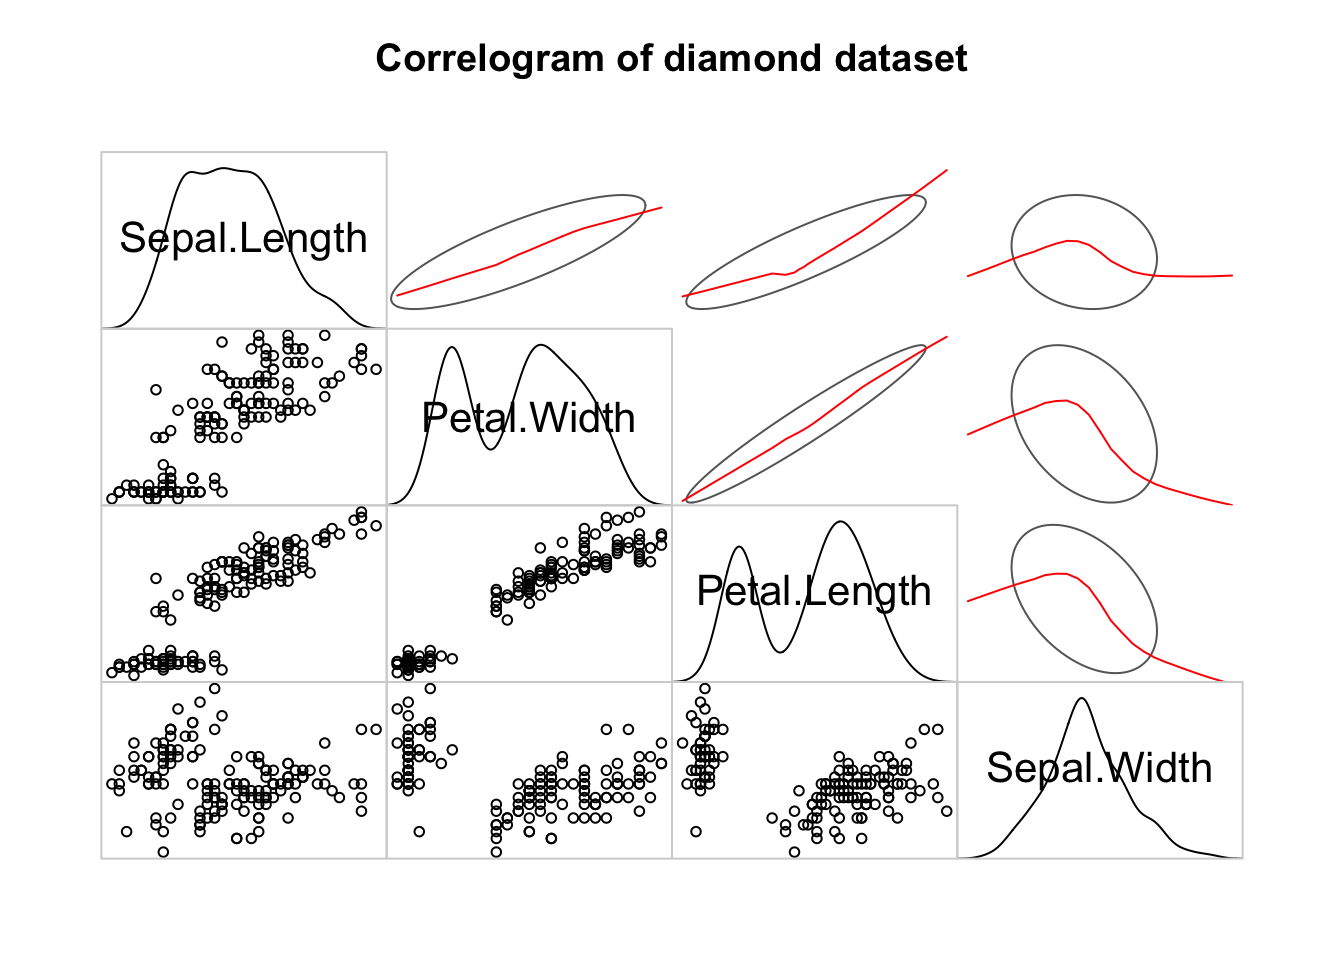
\includegraphics{main_files/figure-latex/unnamed-chunk-166-1.pdf}

\subsection{Kuidas uurida muutuja sisest
varieeruvust}\label{kuidas-uurida-muutuja-sisest-varieeruvust}

Muutuja - midagi, mida mõõdeti (näiteks mõõteobjektide kaal). Kui iga
muutuja kohta on vaid üks number, mida plottida, kasuta Cleveland
plotti:

\begin{Shaded}
\begin{Highlighting}[]
\NormalTok{dd <-}\StringTok{ }\NormalTok{diamonds }\OperatorTok\StringTok{ }\KeywordTok{group_by}\NormalTok{(clarity) }\OperatorTok\StringTok{ }\KeywordTok{summarise}\NormalTok{(}\DataTypeTok{number_of_diamonds=}\KeywordTok{n}\NormalTok{())}
\NormalTok{dd }\OperatorTok\StringTok{ }\KeywordTok{ggplot}\NormalTok{(}\KeywordTok{aes}\NormalTok{(}\DataTypeTok{x=}\NormalTok{number_of_diamonds, }
                  \DataTypeTok{y=}\KeywordTok{reorder}\NormalTok{(clarity, number_of_diamonds))) }\OperatorTok{+}
\StringTok{  }\KeywordTok{geom_point}\NormalTok{(}\DataTypeTok{size=}\DecValTok{3}\NormalTok{) }\OperatorTok{+}
\StringTok{  }\KeywordTok{theme_bw}\NormalTok{() }\OperatorTok{+}
\StringTok{  }\KeywordTok{theme}\NormalTok{(}\DataTypeTok{panel.grid.major.x =} \KeywordTok{element_blank}\NormalTok{(),}
        \DataTypeTok{panel.grid.minor.x =} \KeywordTok{element_blank}\NormalTok{(),}
        \DataTypeTok{panel.grid.major.y =} \KeywordTok{element_line}\NormalTok{(}\DataTypeTok{colour=}\StringTok{"grey60"}\NormalTok{, }\DataTypeTok{linetype=}\StringTok{"dashed"}\NormalTok{)) }\OperatorTok{+}
\StringTok{  }\KeywordTok{labs}\NormalTok{(}\DataTypeTok{y=}\StringTok{"clarity"}\NormalTok{)}
\end{Highlighting}
\end{Shaded}

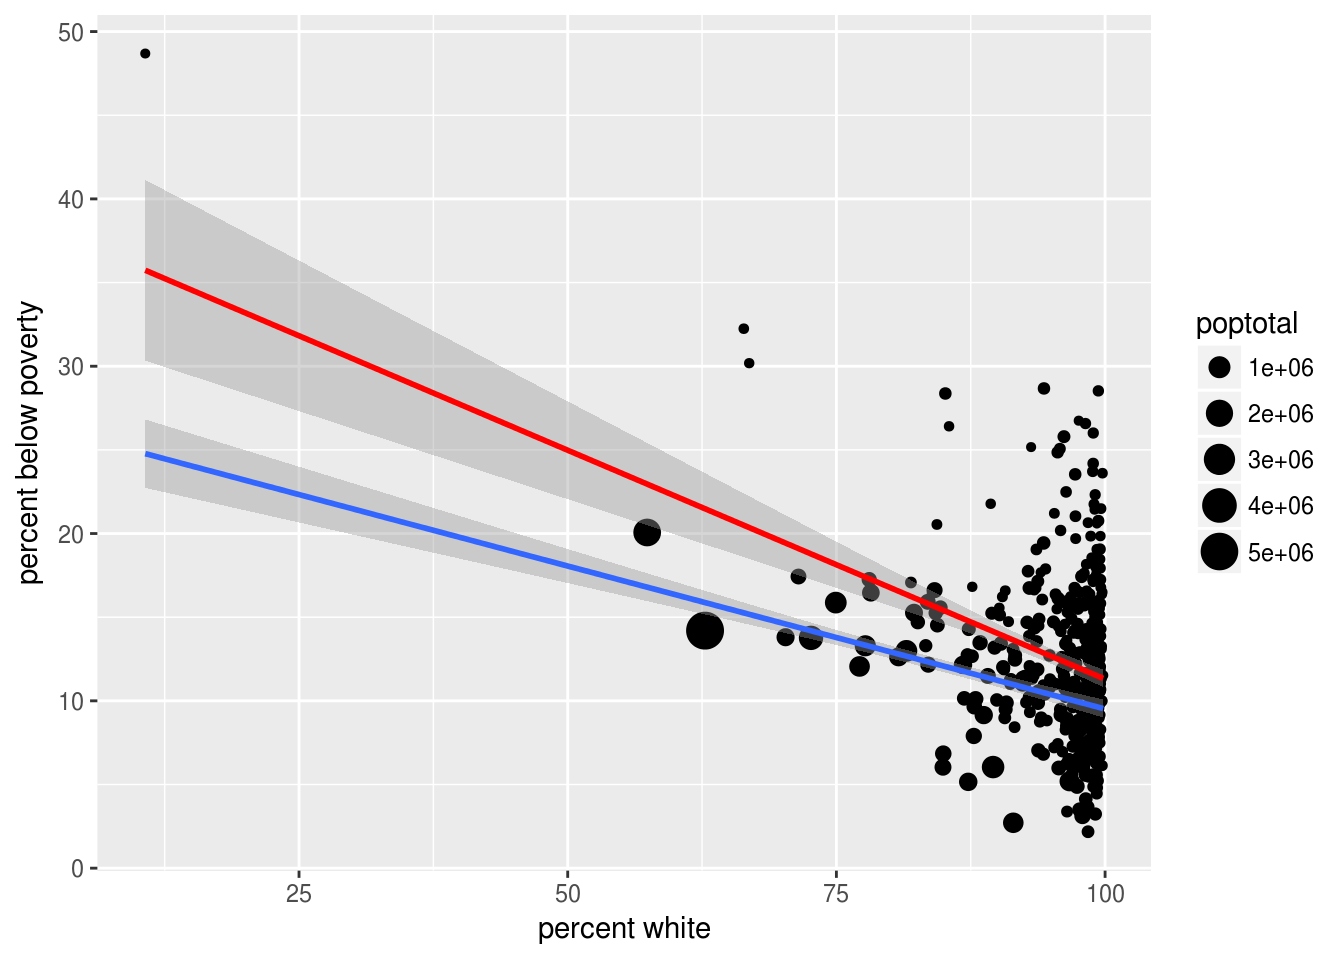
\includegraphics{main_files/figure-latex/unnamed-chunk-167-1.pdf}

\subsubsection{Ploti valik sõltub valimi
suurusest.}\label{ploti-valik-soltub-valimi-suurusest.}

\begin{enumerate}
\def\labelenumi{\arabic{enumi})}
\item
  N \textless{} 20 - ploti iga andmepunkt eraldi (stripchart(), plot())
  ja keskmine või mediaan.
\item
  20 \textgreater{} N \textgreater{} 100: geom\_dotplot() histogrammi
  vaates
\item
  N \textgreater{} 100: geom\_histogram(), geom\_density() --- nende
  abil saab ka 2 kuni 6 jaotust võrrelda
\item
  Mitme jaotuse kõrvuti vaatamiseks kui N \textgreater{} 15:
  geom\_boxplot() or, when N \textgreater{} 50, geom\_violin(),
  geom\_joy()
\end{enumerate}

\begin{Shaded}
\begin{Highlighting}[]
\NormalTok{ToothGrowth <-}\StringTok{ }\NormalTok{ToothGrowth}
\NormalTok{ToothGrowth}\OperatorTok{$}\NormalTok{dose <-}\StringTok{ }\KeywordTok{as.factor}\NormalTok{(ToothGrowth}\OperatorTok{$}\NormalTok{dose)}
\NormalTok{p<-}\KeywordTok{ggplot}\NormalTok{(ToothGrowth, }\KeywordTok{aes}\NormalTok{(}\DataTypeTok{x=}\NormalTok{dose, }\DataTypeTok{y=}\NormalTok{len)) }\OperatorTok{+}\StringTok{ }
\StringTok{  }\KeywordTok{geom_dotplot}\NormalTok{(}\DataTypeTok{binaxis=}\StringTok{'y'}\NormalTok{, }\DataTypeTok{stackdir=}\StringTok{'center'}\NormalTok{)}
\NormalTok{p}
\end{Highlighting}
\end{Shaded}

\begin{verbatim}
## `stat_bindot()` using `bins = 30`. Pick better value with `binwidth`.
\end{verbatim}

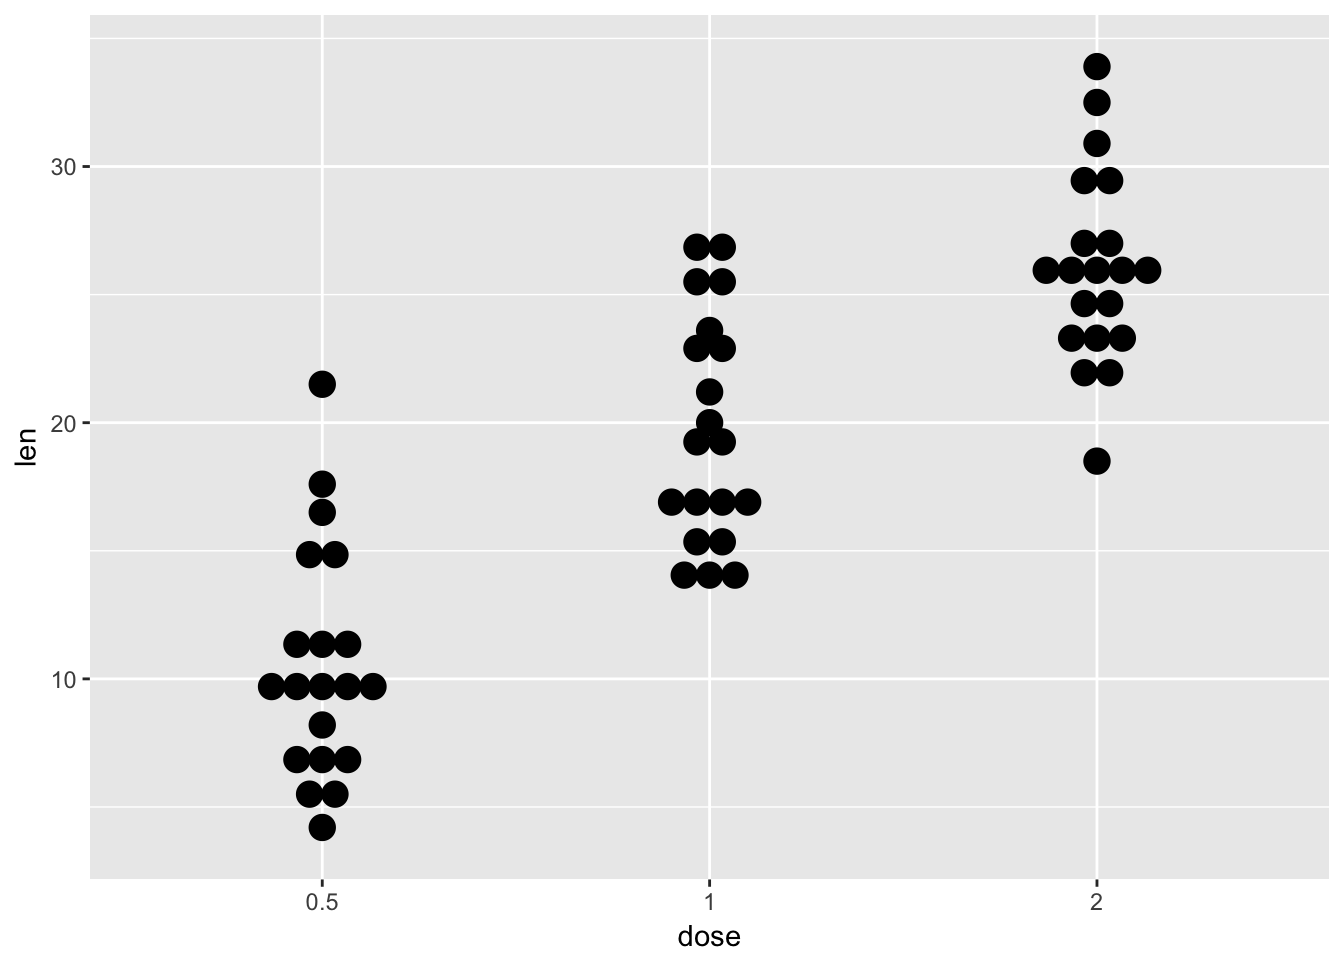
\includegraphics{main_files/figure-latex/unnamed-chunk-168-1.pdf}

\begin{Shaded}
\begin{Highlighting}[]
\CommentTok{# Change dotsize and stack ratio, add line or dot for median}
\KeywordTok{ggplot}\NormalTok{(ToothGrowth, }\KeywordTok{aes}\NormalTok{(}\DataTypeTok{x=}\NormalTok{dose, }\DataTypeTok{y=}\NormalTok{len)) }\OperatorTok{+}\StringTok{ }
\StringTok{  }\KeywordTok{geom_dotplot}\NormalTok{(}\DataTypeTok{binaxis=}\StringTok{'y'}\NormalTok{, }\DataTypeTok{stackdir=}\StringTok{'center'}\NormalTok{,}
               \DataTypeTok{stackratio=}\FloatTok{1.5}\NormalTok{, }\DataTypeTok{dotsize=}\FloatTok{0.7}\NormalTok{)}\OperatorTok{+}
\StringTok{  }\KeywordTok{stat_summary}\NormalTok{(}\DataTypeTok{fun.y =}\NormalTok{ median, }\DataTypeTok{geom =} \StringTok{"point"}\NormalTok{, }\DataTypeTok{shape =} \DecValTok{95}\NormalTok{, }
               \DataTypeTok{color =} \StringTok{"red"}\NormalTok{, }\DataTypeTok{size =} \DecValTok{15}\NormalTok{) }\OperatorTok{+}
\StringTok{  }\KeywordTok{theme_tufte}\NormalTok{()}
\end{Highlighting}
\end{Shaded}

\begin{verbatim}
## `stat_bindot()` using `bins = 30`. Pick better value with `binwidth`.
\end{verbatim}

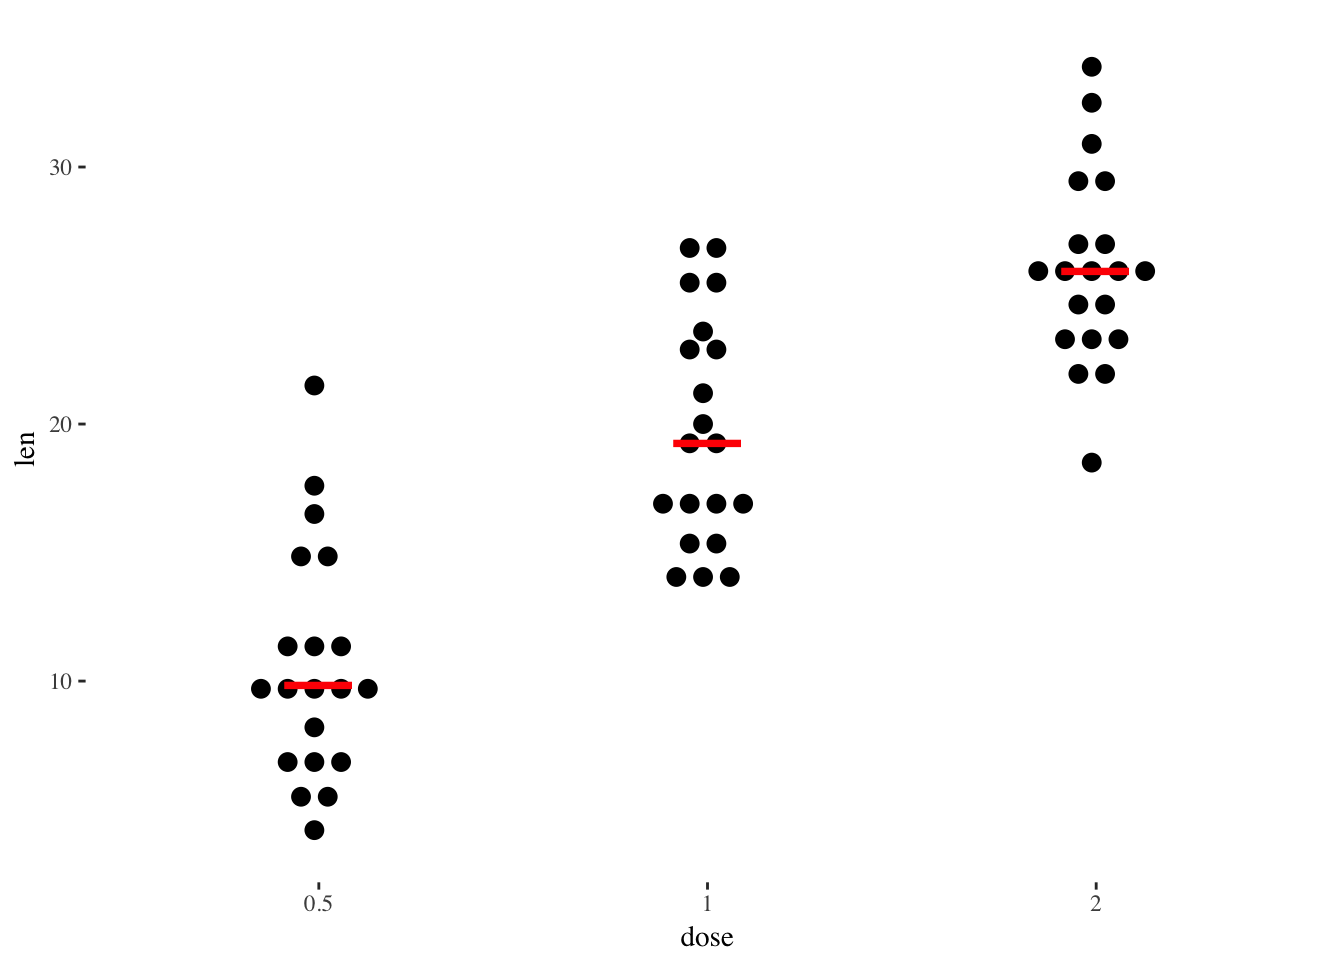
\includegraphics{main_files/figure-latex/unnamed-chunk-168-2.pdf}

\begin{Shaded}
\begin{Highlighting}[]
\NormalTok{p }\OperatorTok{+}\StringTok{ }\KeywordTok{stat_summary}\NormalTok{(}\DataTypeTok{fun.y=}\NormalTok{median, }\DataTypeTok{geom=}\StringTok{"point"}\NormalTok{, }\DataTypeTok{shape=}\DecValTok{18}\NormalTok{,}
                 \DataTypeTok{size=}\DecValTok{5}\NormalTok{, }\DataTypeTok{color=}\StringTok{"red"}\NormalTok{)}
\end{Highlighting}
\end{Shaded}

\begin{verbatim}
## `stat_bindot()` using `bins = 30`. Pick better value with `binwidth`.
\end{verbatim}

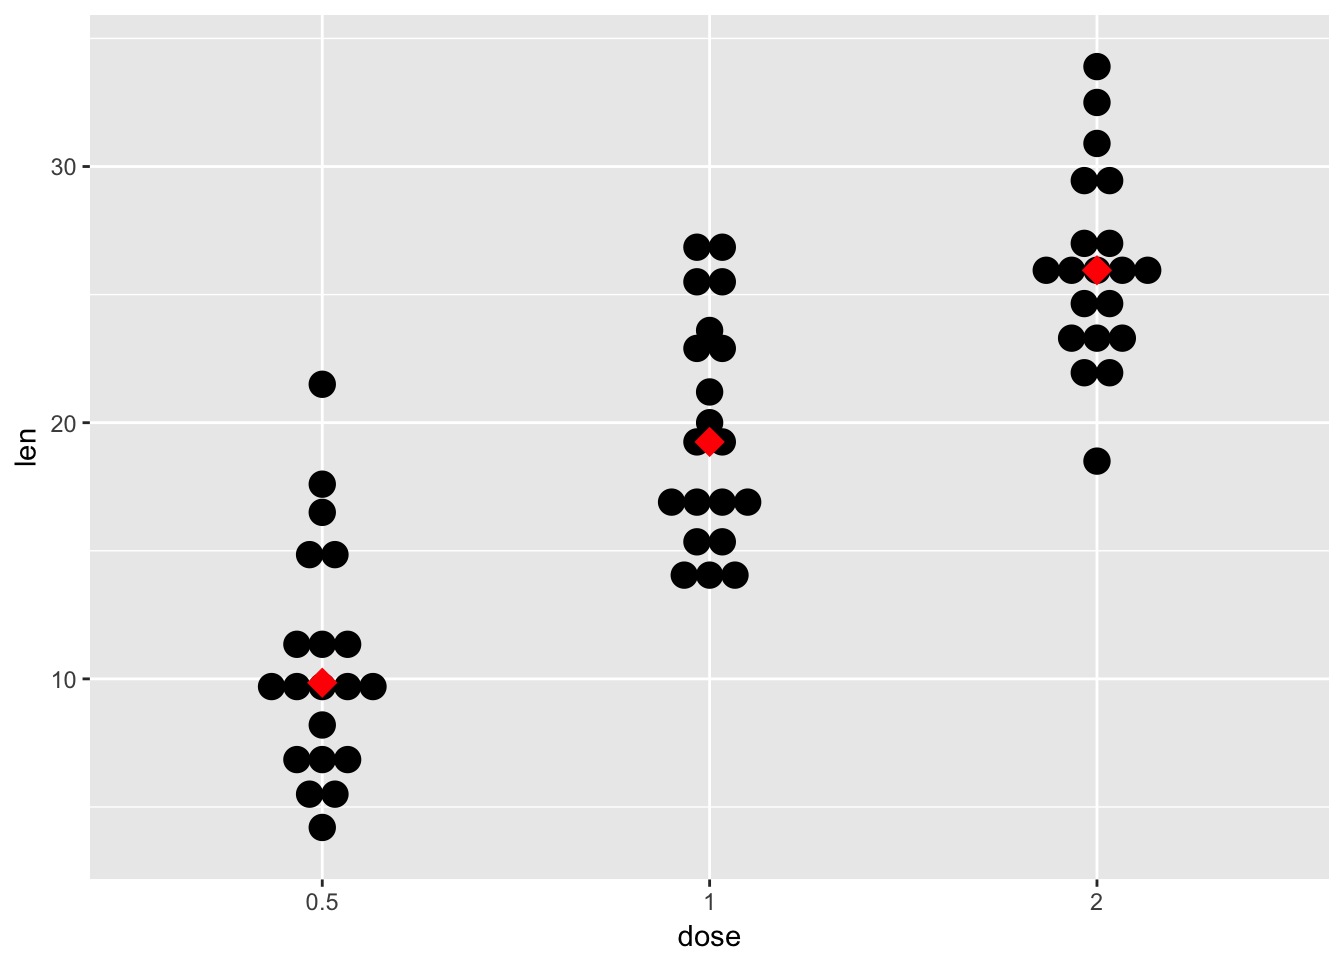
\includegraphics{main_files/figure-latex/unnamed-chunk-168-3.pdf}

\begin{Shaded}
\begin{Highlighting}[]
\CommentTok{#add mean and SD, use pointrange}
\NormalTok{p }\OperatorTok{+}\StringTok{ }\KeywordTok{stat_summary}\NormalTok{(}\DataTypeTok{fun.data=}\NormalTok{mean_sdl, }\DataTypeTok{fun.args =} \KeywordTok{list}\NormalTok{(}\DataTypeTok{mult=}\DecValTok{1}\NormalTok{), }
                 \DataTypeTok{geom=}\StringTok{"pointrange"}\NormalTok{, }\DataTypeTok{color=}\StringTok{"red"}\NormalTok{)}
\end{Highlighting}
\end{Shaded}

\begin{verbatim}
## `stat_bindot()` using `bins = 30`. Pick better value with `binwidth`.
\end{verbatim}

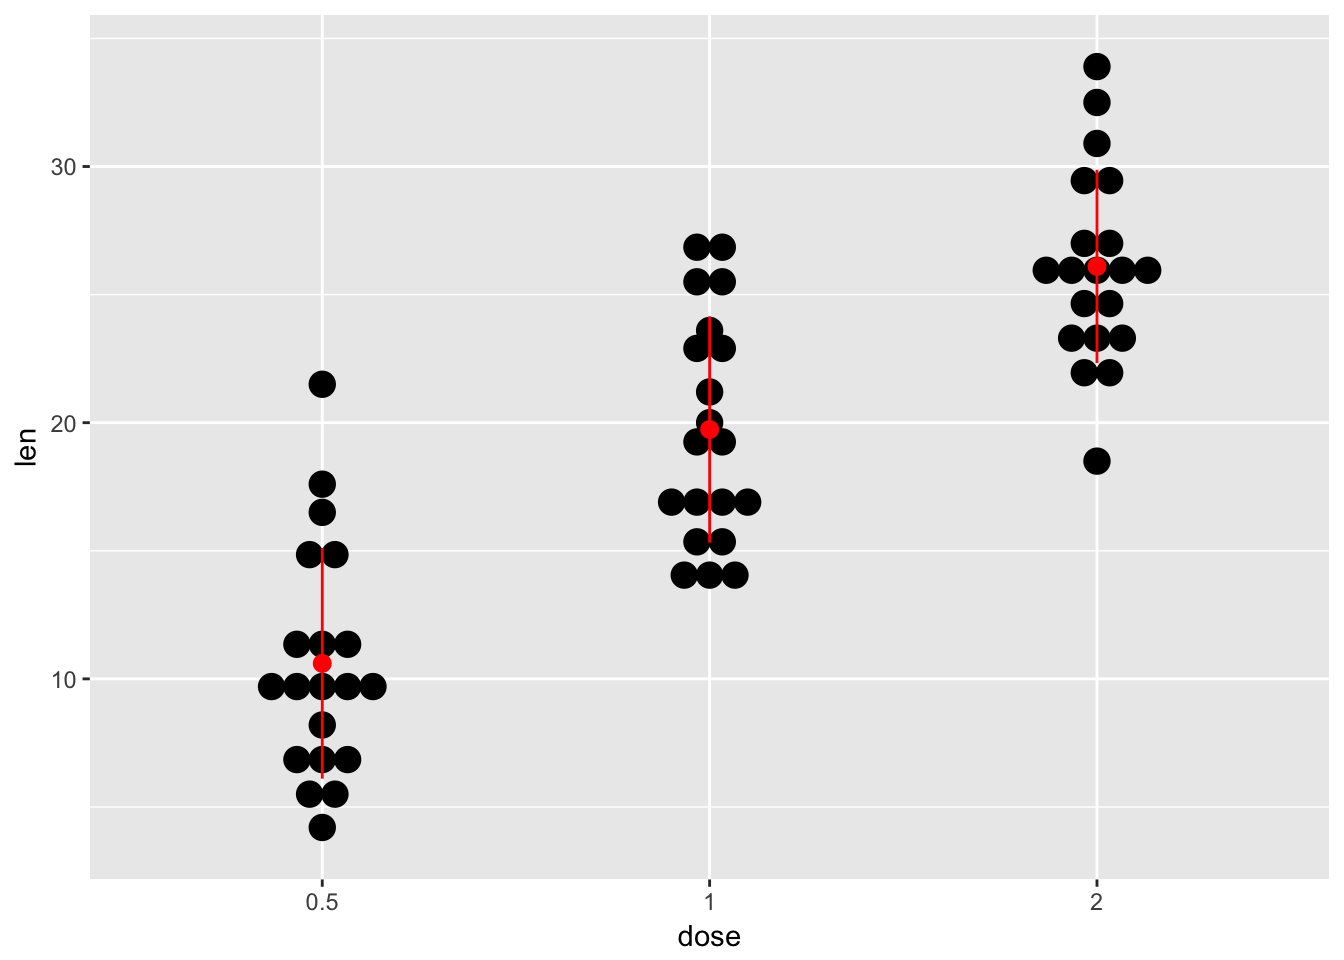
\includegraphics{main_files/figure-latex/unnamed-chunk-168-4.pdf}

\begin{Shaded}
\begin{Highlighting}[]
\CommentTok{#use errorbars}
\NormalTok{p }\OperatorTok{+}\StringTok{ }\KeywordTok{stat_summary}\NormalTok{(}\DataTypeTok{fun.data=}\NormalTok{mean_sdl, }\DataTypeTok{fun.args =} \KeywordTok{list}\NormalTok{(}\DataTypeTok{mult=}\DecValTok{1}\NormalTok{), }
        \DataTypeTok{geom=}\StringTok{"errorbar"}\NormalTok{, }\DataTypeTok{color=}\StringTok{"red"}\NormalTok{, }\DataTypeTok{width=}\FloatTok{0.2}\NormalTok{) }\OperatorTok{+}
\StringTok{  }\KeywordTok{stat_summary}\NormalTok{(}\DataTypeTok{fun.y=}\NormalTok{mean, }\DataTypeTok{geom=}\StringTok{"point"}\NormalTok{, }\DataTypeTok{size=}\DecValTok{3}\NormalTok{, }\DataTypeTok{color=}\StringTok{"red"}\NormalTok{)}
\end{Highlighting}
\end{Shaded}

\begin{verbatim}
## `stat_bindot()` using `bins = 30`. Pick better value with `binwidth`.
\end{verbatim}

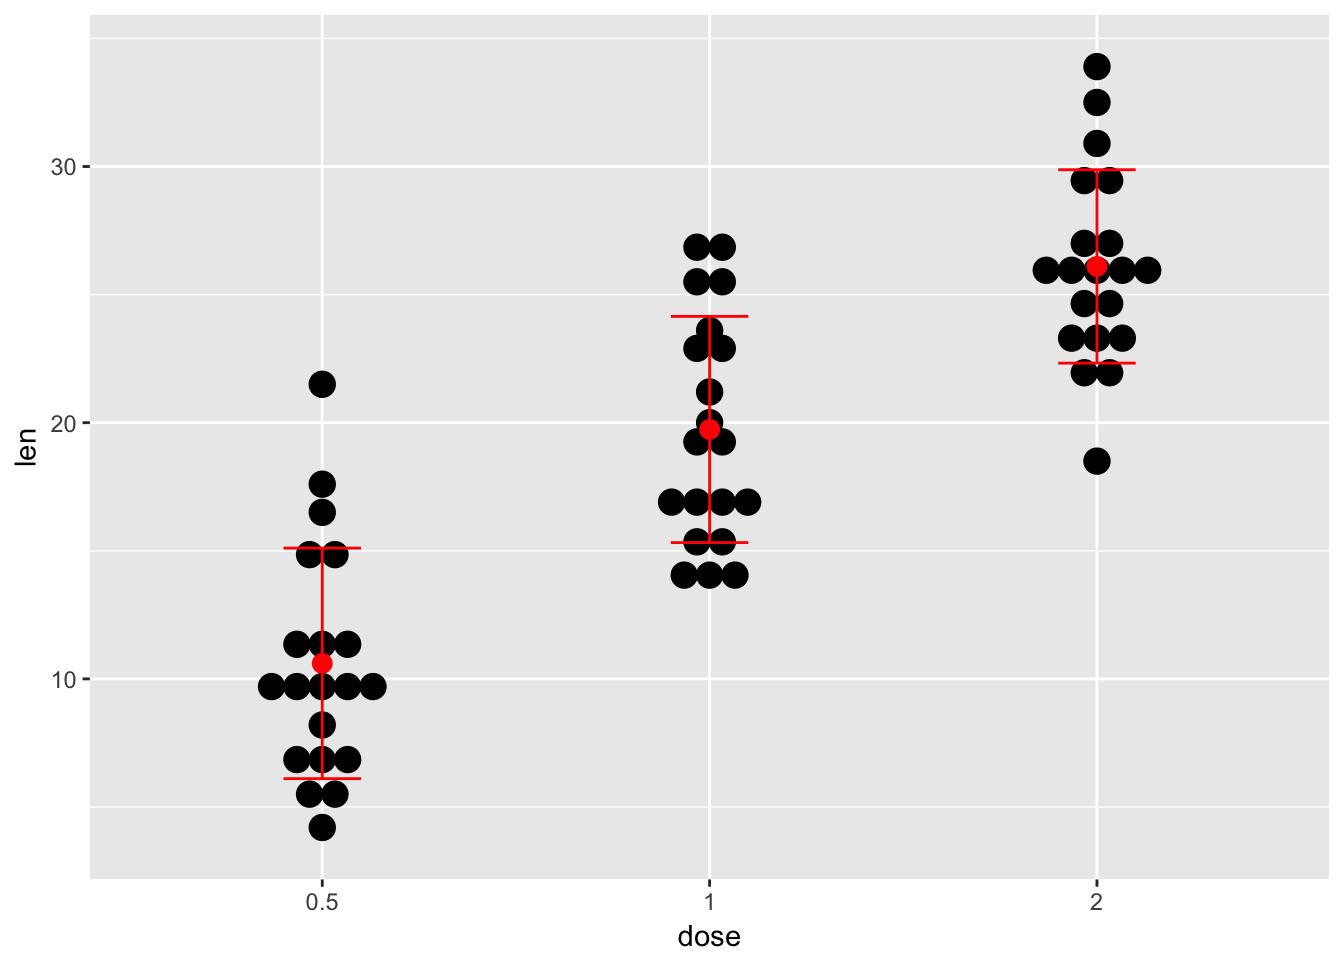
\includegraphics{main_files/figure-latex/unnamed-chunk-168-5.pdf}

Use a custom summary function :

\begin{Shaded}
\begin{Highlighting}[]
\CommentTok{# Function to produce summary statistics (geometric mean and multipülicative sd)}
\NormalTok{multi_sd <-}\StringTok{ }\ControlFlowTok{function}\NormalTok{(x) \{}
\NormalTok{  x <-}\StringTok{ }\KeywordTok{na.omit}\NormalTok{(x)}
\NormalTok{  a <-}\StringTok{ }\KeywordTok{log10}\NormalTok{(x)}
\NormalTok{  b <-}\StringTok{ }\KeywordTok{mean}\NormalTok{(a)}
\NormalTok{  c <-}\StringTok{ }\KeywordTok{sd}\NormalTok{(a)}
\NormalTok{  g_mean <-}\StringTok{ }\DecValTok{10}\OperatorTok{**}\NormalTok{b}
\NormalTok{  msd <-}\StringTok{ }\DecValTok{10}\OperatorTok{**}\NormalTok{c}
\NormalTok{  ymin <-}\StringTok{ }\NormalTok{g_mean}\OperatorTok{/}\NormalTok{msd}
\NormalTok{  ymax <-}\StringTok{ }\NormalTok{g_mean }\OperatorTok{*}\StringTok{ }\NormalTok{msd}
 \KeywordTok{return}\NormalTok{(}\KeywordTok{c}\NormalTok{(}\DataTypeTok{y =}\NormalTok{ g_mean, }\DataTypeTok{ymin =}\NormalTok{ ymin, }\DataTypeTok{ymax =}\NormalTok{ ymax)) }
\NormalTok{\}}
\NormalTok{p }\OperatorTok{+}\StringTok{ }\KeywordTok{stat_summary}\NormalTok{(}\DataTypeTok{fun.data=}\NormalTok{multi_sd, }\DataTypeTok{color=}\StringTok{"blue"}\NormalTok{, }\DataTypeTok{size=}\FloatTok{1.1}\NormalTok{) }\OperatorTok{+}\StringTok{ }\KeywordTok{theme_tufte}\NormalTok{()}
\end{Highlighting}
\end{Shaded}

\begin{verbatim}
## `stat_bindot()` using `bins = 30`. Pick better value with `binwidth`.
\end{verbatim}

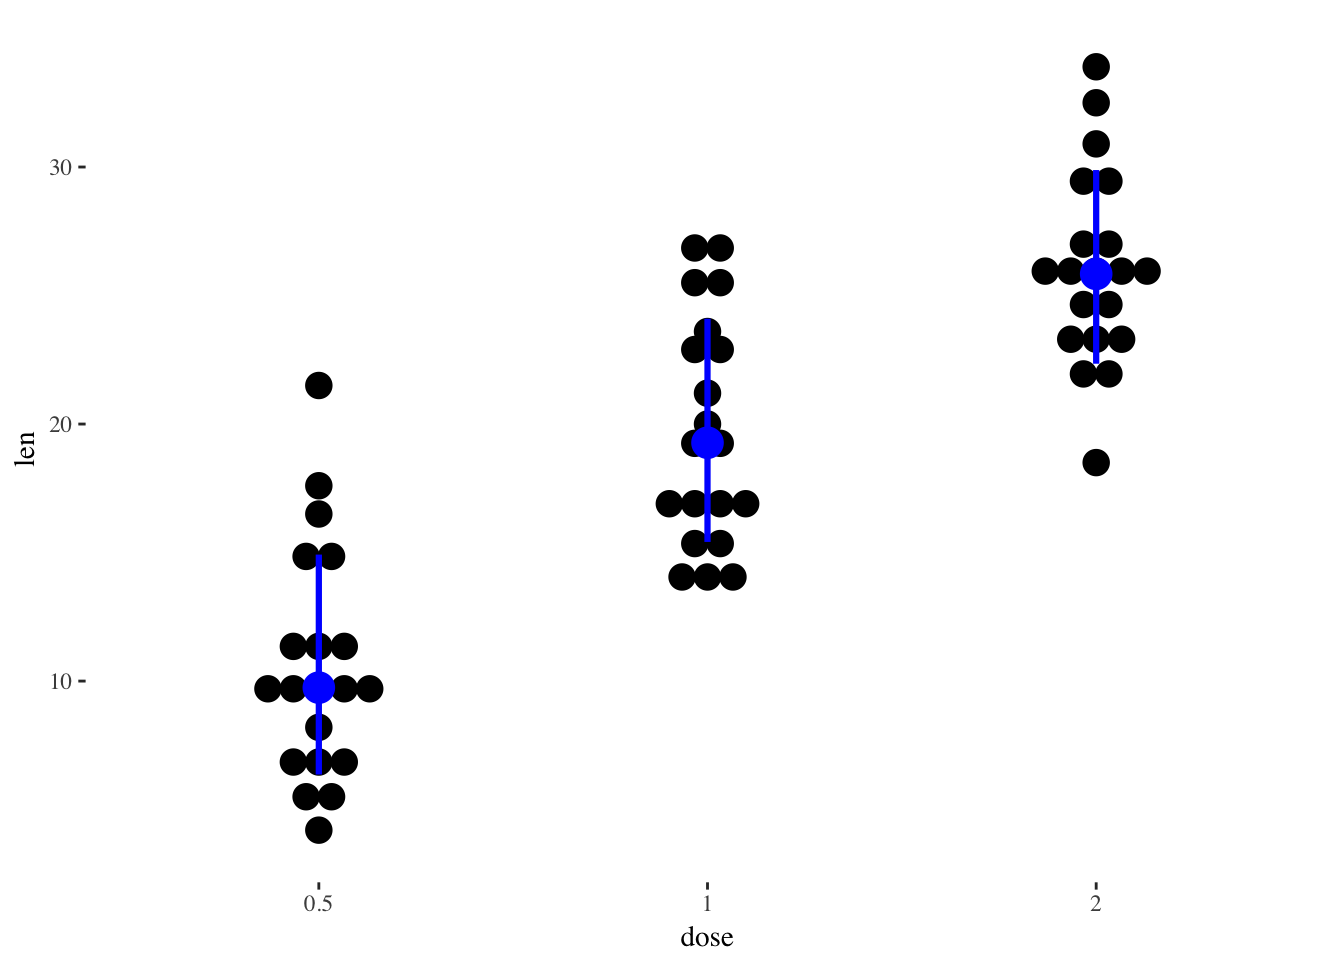
\includegraphics{main_files/figure-latex/unnamed-chunk-170-1.pdf}

\begin{Shaded}
\begin{Highlighting}[]
\CommentTok{# Change dot plot colors by groups}
\NormalTok{p<-}\KeywordTok{ggplot}\NormalTok{(ToothGrowth, }\KeywordTok{aes}\NormalTok{(}\DataTypeTok{x=}\NormalTok{dose, }\DataTypeTok{y=}\NormalTok{len, }\DataTypeTok{fill=}\NormalTok{dose)) }\OperatorTok{+}
\StringTok{  }\KeywordTok{geom_dotplot}\NormalTok{(}\DataTypeTok{binaxis=}\StringTok{'y'}\NormalTok{, }\DataTypeTok{stackdir=}\StringTok{'center'}\NormalTok{)}
\NormalTok{p}
\end{Highlighting}
\end{Shaded}

\begin{verbatim}
## `stat_bindot()` using `bins = 30`. Pick better value with `binwidth`.
\end{verbatim}

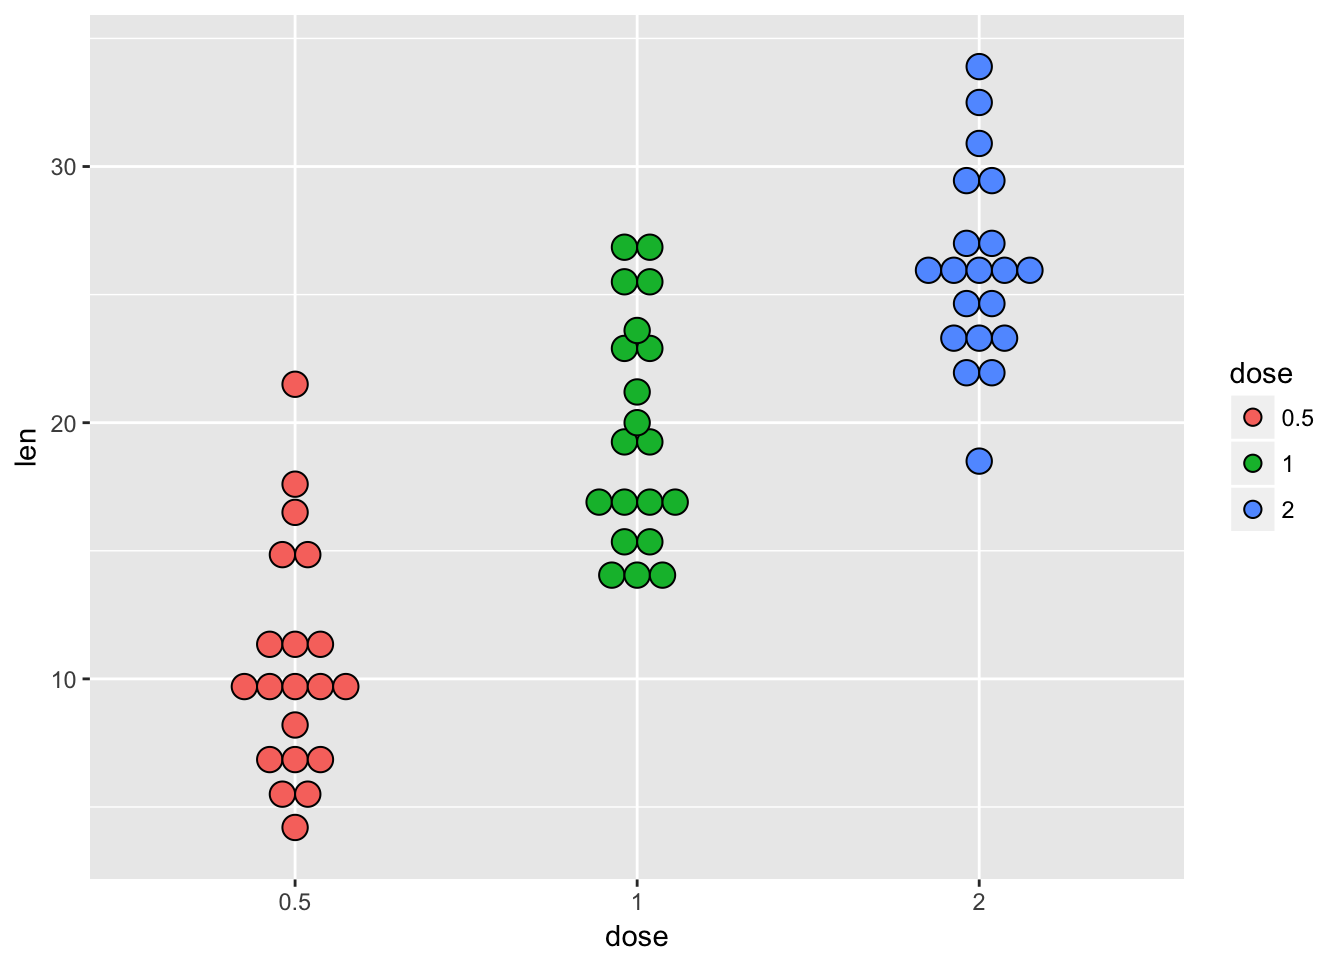
\includegraphics{main_files/figure-latex/unnamed-chunk-171-1.pdf}

It is also possible to change manually dot plot colors using the
functions :

scale\_fill\_manual() : to use custom colors

scale\_fill\_brewer() : to use color palettes from RColorBrewer package

scale\_fill\_grey() : to use grey color palettes

\begin{Shaded}
\begin{Highlighting}[]
\CommentTok{#Choose which items to display :}
\NormalTok{p }\OperatorTok{+}\StringTok{ }\KeywordTok{scale_x_discrete}\NormalTok{(}\DataTypeTok{limits=}\KeywordTok{c}\NormalTok{(}\StringTok{"0.5"}\NormalTok{, }\StringTok{"2"}\NormalTok{))}
\end{Highlighting}
\end{Shaded}

\begin{verbatim}
## `stat_bindot()` using `bins = 30`. Pick better value with `binwidth`.
\end{verbatim}

\begin{verbatim}
## Warning: Removed 20 rows containing non-finite values (stat_bindot).
\end{verbatim}

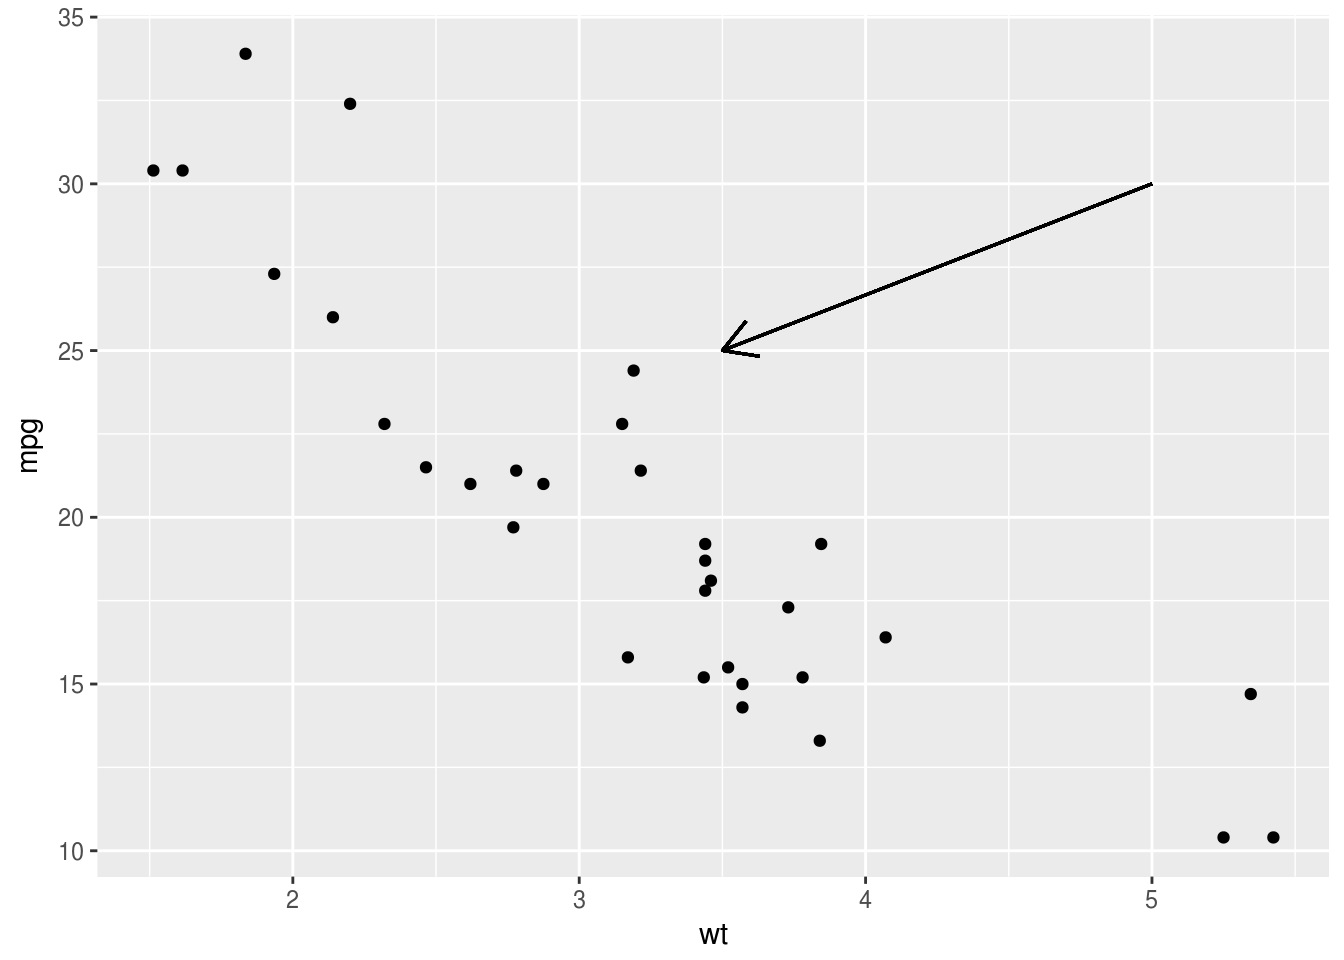
\includegraphics{main_files/figure-latex/unnamed-chunk-172-1.pdf}

Dotplot kui histogram:

\begin{Shaded}
\begin{Highlighting}[]
\KeywordTok{ggplot}\NormalTok{(iris, }\KeywordTok{aes}\NormalTok{(Sepal.Length)) }\OperatorTok{+}\StringTok{ }\KeywordTok{geom_dotplot}\NormalTok{()}
\end{Highlighting}
\end{Shaded}

\begin{verbatim}
## `stat_bindot()` using `bins = 30`. Pick better value with `binwidth`.
\end{verbatim}

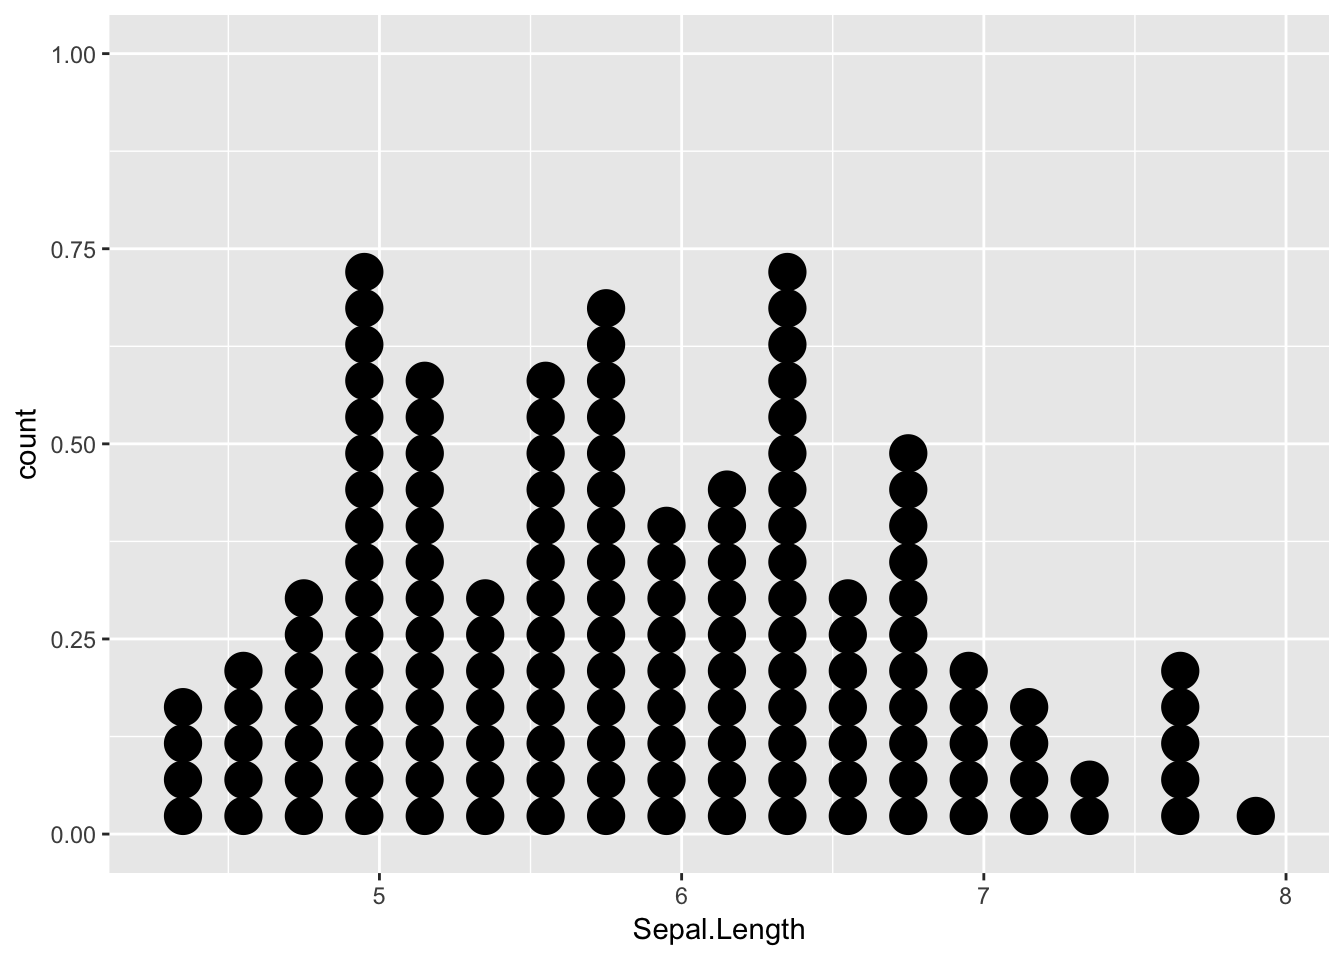
\includegraphics{main_files/figure-latex/unnamed-chunk-173-1.pdf}

Histogram:

\begin{Shaded}
\begin{Highlighting}[]
\KeywordTok{ggplot}\NormalTok{(iris, }\KeywordTok{aes}\NormalTok{(Sepal.Length)) }\OperatorTok{+}\StringTok{ }
\StringTok{  }\KeywordTok{geom_histogram}\NormalTok{(}\DataTypeTok{bins =} \DecValTok{10}\NormalTok{, }\DataTypeTok{color=}\StringTok{"white"}\NormalTok{, }\DataTypeTok{fill =} \StringTok{"navyblue"}\NormalTok{) }
\end{Highlighting}
\end{Shaded}

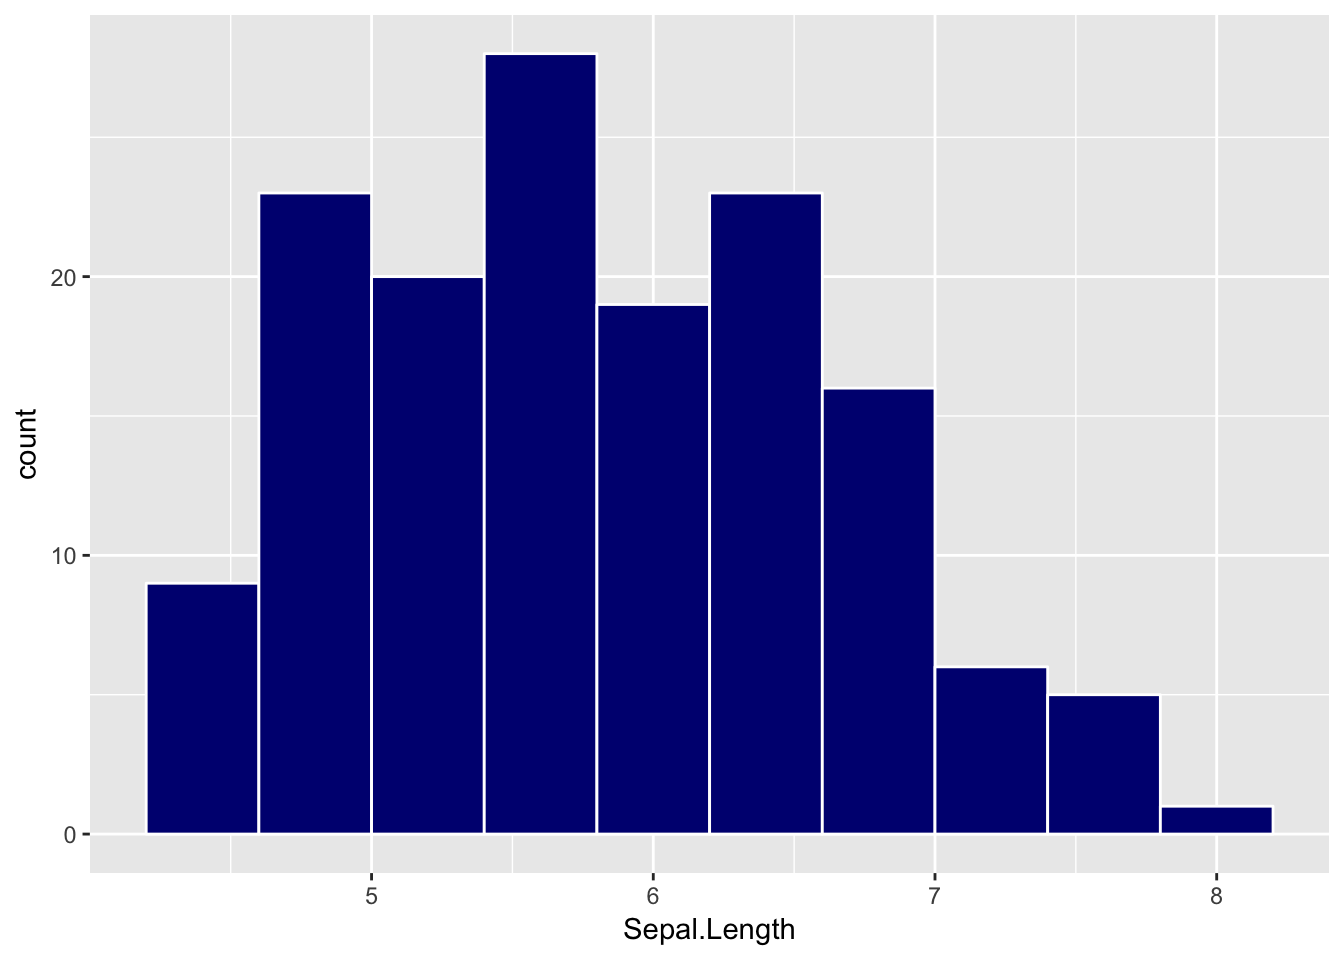
\includegraphics{main_files/figure-latex/unnamed-chunk-174-1.pdf}

\begin{Shaded}
\begin{Highlighting}[]
\KeywordTok{library}\NormalTok{(ggthemes)}
\NormalTok{d <-}\StringTok{ }\NormalTok{iris        }\CommentTok{# Full data set}
\NormalTok{d_bg <-}\StringTok{ }\NormalTok{d[, }\OperatorTok{-}\DecValTok{5}\NormalTok{]  }\CommentTok{# Background Data - full without the 5th column (Species)}

\KeywordTok{ggplot}\NormalTok{(}\DataTypeTok{data =}\NormalTok{ d, }\KeywordTok{aes}\NormalTok{(}\DataTypeTok{x =}\NormalTok{ Sepal.Width, }\DataTypeTok{fill =}\NormalTok{ Species)) }\OperatorTok{+}
\StringTok{  }\KeywordTok{geom_histogram}\NormalTok{(}\DataTypeTok{data =}\NormalTok{ d_bg, }\DataTypeTok{fill =} \StringTok{"grey"}\NormalTok{, }\DataTypeTok{alpha=}\FloatTok{0.8}\NormalTok{, }\DataTypeTok{bins=}\DecValTok{10}\NormalTok{) }\OperatorTok{+}
\StringTok{  }\KeywordTok{geom_histogram}\NormalTok{(}\DataTypeTok{colour =} \StringTok{"black"}\NormalTok{, }\DataTypeTok{bins=}\DecValTok{10}\NormalTok{) }\OperatorTok{+}
\StringTok{  }\KeywordTok{facet_grid}\NormalTok{(Species}\OperatorTok{~}\NormalTok{.) }\OperatorTok{+}
\StringTok{  }\KeywordTok{guides}\NormalTok{(}\DataTypeTok{fill =} \OtherTok{FALSE}\NormalTok{) }\OperatorTok{+}\StringTok{  }\CommentTok{# to remove the legend}
\StringTok{  }\KeywordTok{theme_tufte}\NormalTok{()          }\CommentTok{# for clean look overall}
\end{Highlighting}
\end{Shaded}

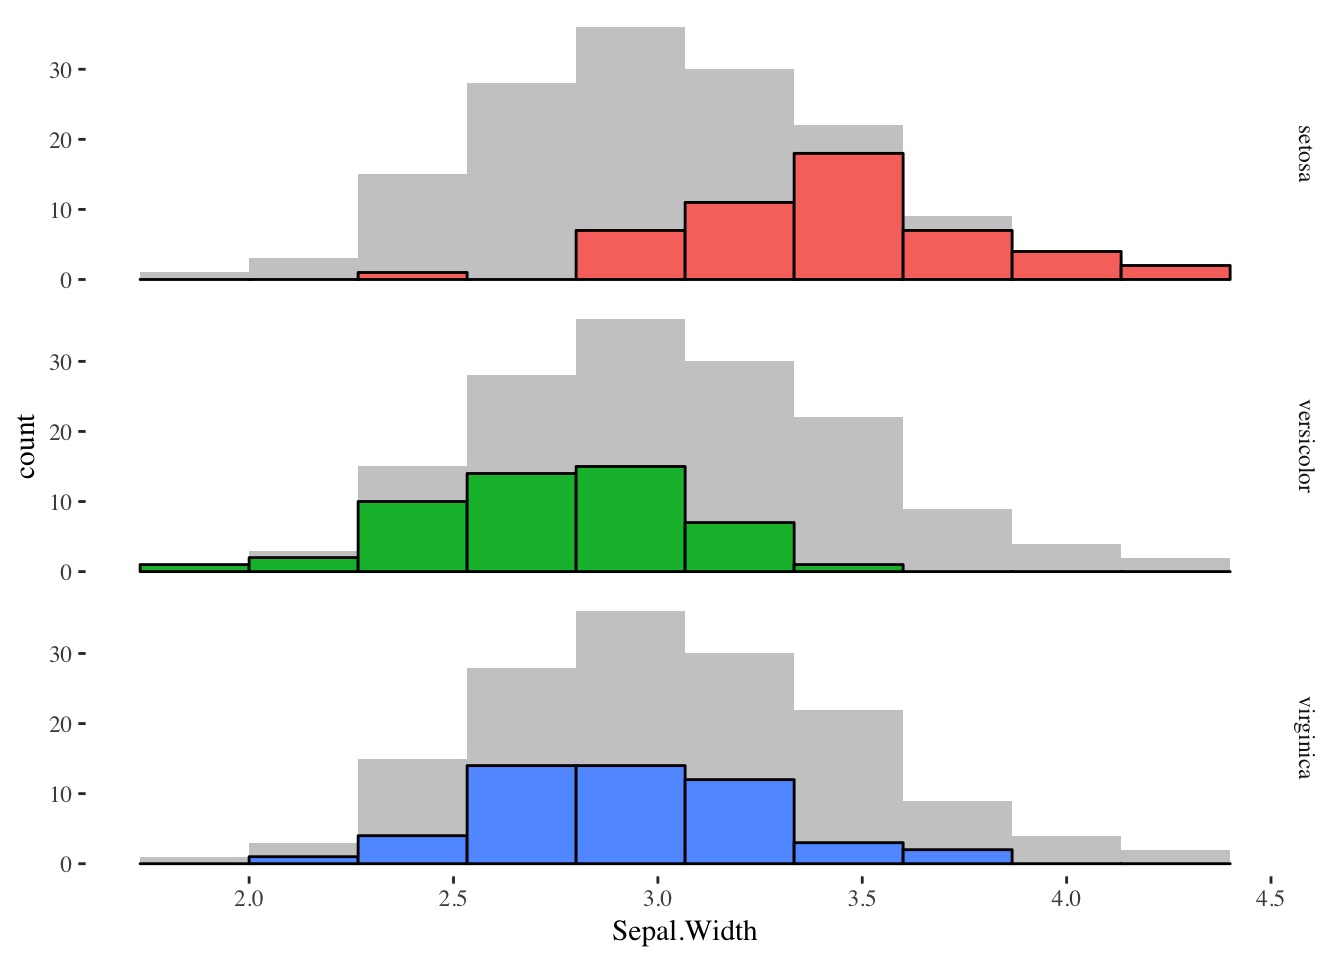
\includegraphics{main_files/figure-latex/unnamed-chunk-175-1.pdf}

density plot:

\begin{Shaded}
\begin{Highlighting}[]
\NormalTok{iris}\OperatorTok\KeywordTok{ggplot}\NormalTok{()}\OperatorTok{+}
\StringTok{  }\KeywordTok{geom_density}\NormalTok{(}\KeywordTok{aes}\NormalTok{(Sepal.Width, }\DataTypeTok{fill=}\NormalTok{Species, }\DataTypeTok{color=}\NormalTok{Species, }\DataTypeTok{alpha=}\FloatTok{0.5}\NormalTok{))}\OperatorTok{+}
\StringTok{  }\KeywordTok{theme_tufte}\NormalTok{()}
\end{Highlighting}
\end{Shaded}

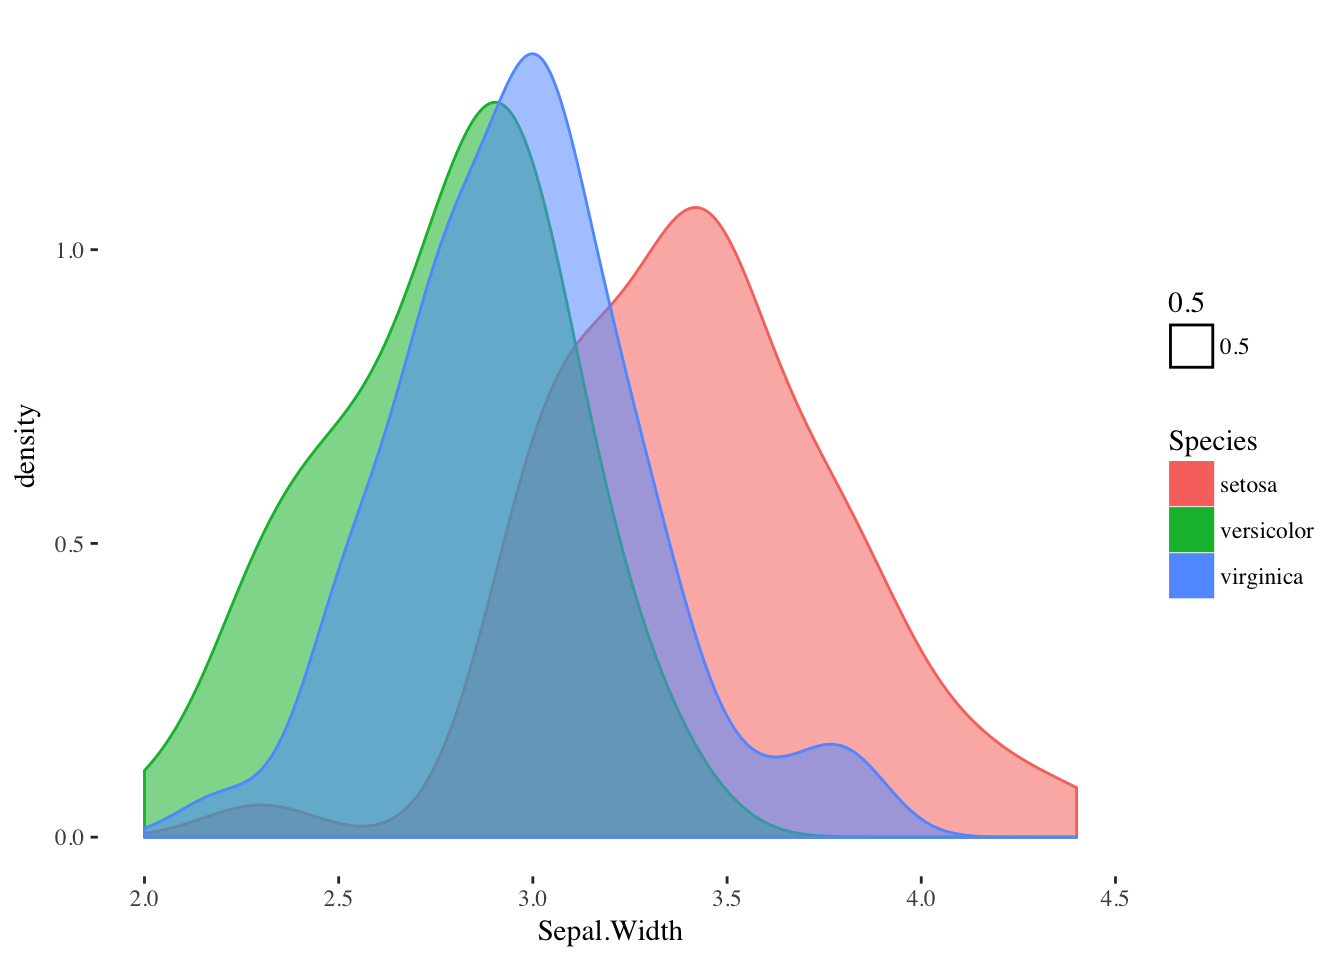
\includegraphics{main_files/figure-latex/unnamed-chunk-176-1.pdf}

joyplot võimaldab kõrvuti panna isegi sadu density plotte

\begin{Shaded}
\begin{Highlighting}[]
\KeywordTok{library}\NormalTok{(ggjoy)}
\KeywordTok{ggplot}\NormalTok{(iris, }\KeywordTok{aes}\NormalTok{(}\DataTypeTok{x=}\NormalTok{Sepal.Length, }\DataTypeTok{y=}\NormalTok{Species, }\DataTypeTok{fill=}\NormalTok{Species)) }\OperatorTok{+}\StringTok{ }
\StringTok{  }\KeywordTok{geom_joy}\NormalTok{(}\DataTypeTok{scale=}\DecValTok{4}\NormalTok{, }\DataTypeTok{rel_min_height=}\FloatTok{0.01}\NormalTok{, }\DataTypeTok{alpha=}\FloatTok{0.9}\NormalTok{) }\OperatorTok{+}
\StringTok{  }\KeywordTok{theme_joy}\NormalTok{(}\DataTypeTok{font_size =} \DecValTok{13}\NormalTok{, }\DataTypeTok{grid=}\OtherTok{TRUE}\NormalTok{) }\OperatorTok{+}\StringTok{ }
\StringTok{  }\KeywordTok{theme}\NormalTok{(}\DataTypeTok{legend.position =} \StringTok{"none"}\NormalTok{)}
\end{Highlighting}
\end{Shaded}

\begin{verbatim}
## Picking joint bandwidth of 0.181
\end{verbatim}

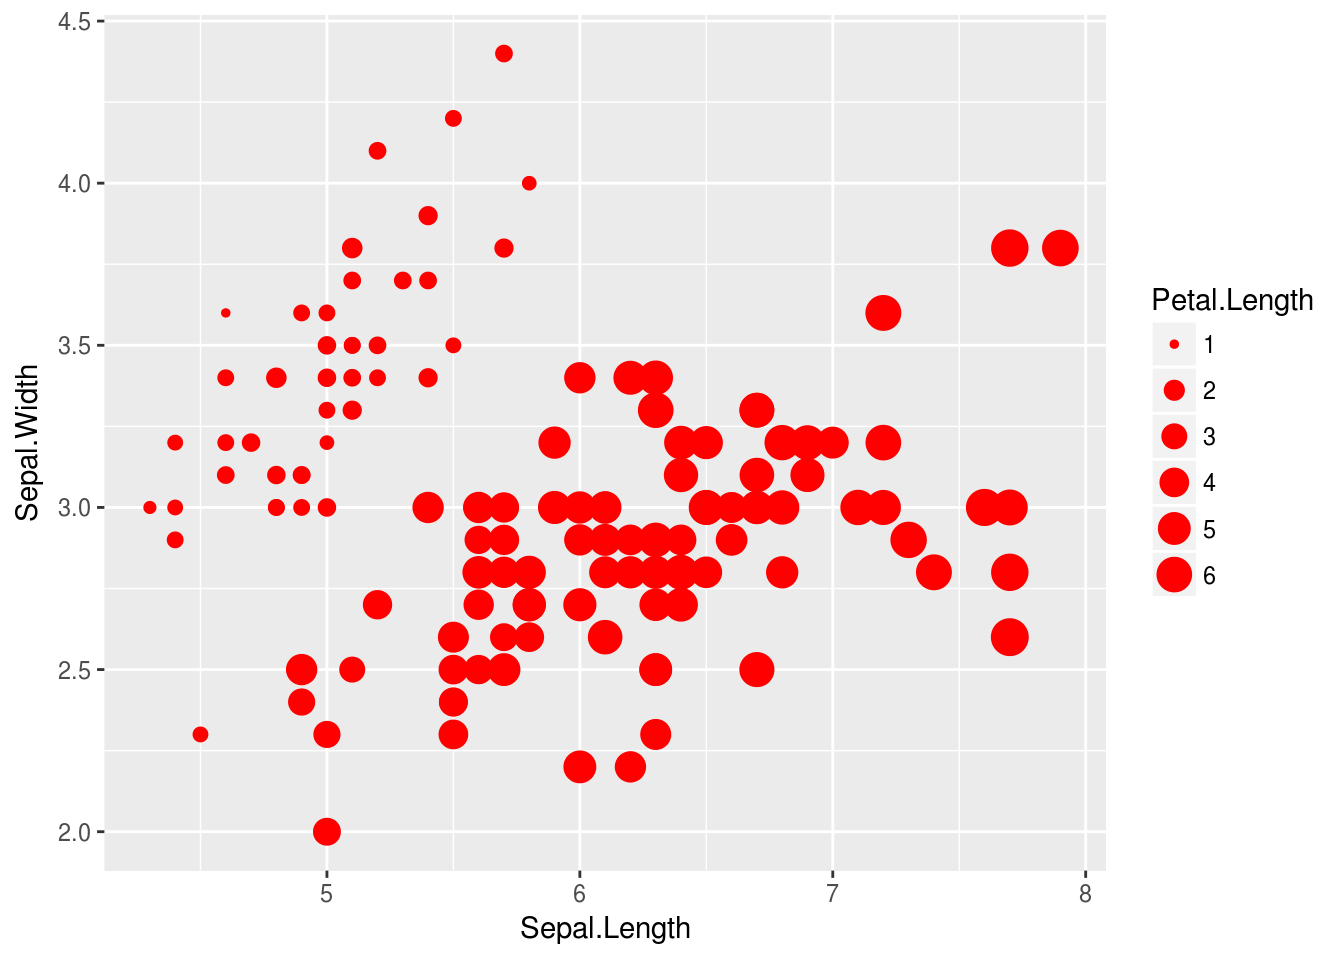
\includegraphics{main_files/figure-latex/unnamed-chunk-177-1.pdf}

Boxplot:

\begin{Shaded}
\begin{Highlighting}[]
\KeywordTok{ggplot}\NormalTok{(iris, }\KeywordTok{aes}\NormalTok{(Species, Sepal.Width, }\DataTypeTok{fill=}\NormalTok{Species)) }\OperatorTok{+}\StringTok{ }\KeywordTok{geom_boxplot}\NormalTok{()}
\end{Highlighting}
\end{Shaded}

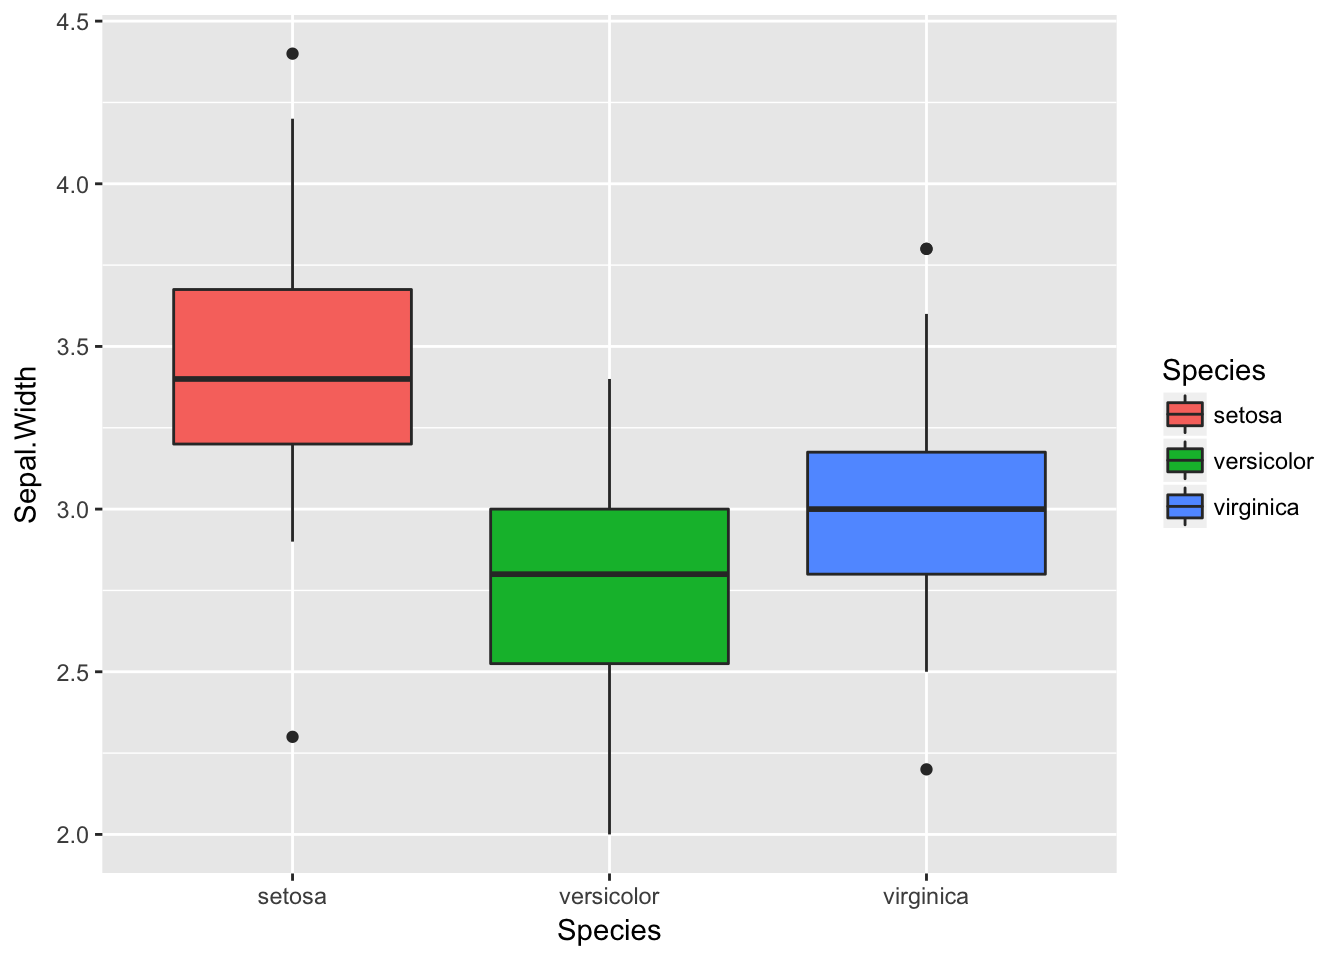
\includegraphics{main_files/figure-latex/unnamed-chunk-178-1.pdf}

violin plot plus jitterplot:

\begin{Shaded}
\begin{Highlighting}[]
\KeywordTok{ggplot}\NormalTok{(iris, }\KeywordTok{aes}\NormalTok{(Species, Sepal.Width)) }\OperatorTok{+}\StringTok{ }
\StringTok{  }\KeywordTok{geom_violin}\NormalTok{(}\KeywordTok{aes}\NormalTok{(}\DataTypeTok{fill=}\NormalTok{Species)) }\OperatorTok{+}
\StringTok{  }\KeywordTok{geom_jitter}\NormalTok{(}\DataTypeTok{width =} \FloatTok{0.1}\NormalTok{, }\DataTypeTok{alpha=}\FloatTok{0.4}\NormalTok{, }\DataTypeTok{size=}\FloatTok{0.5}\NormalTok{)}
\end{Highlighting}
\end{Shaded}

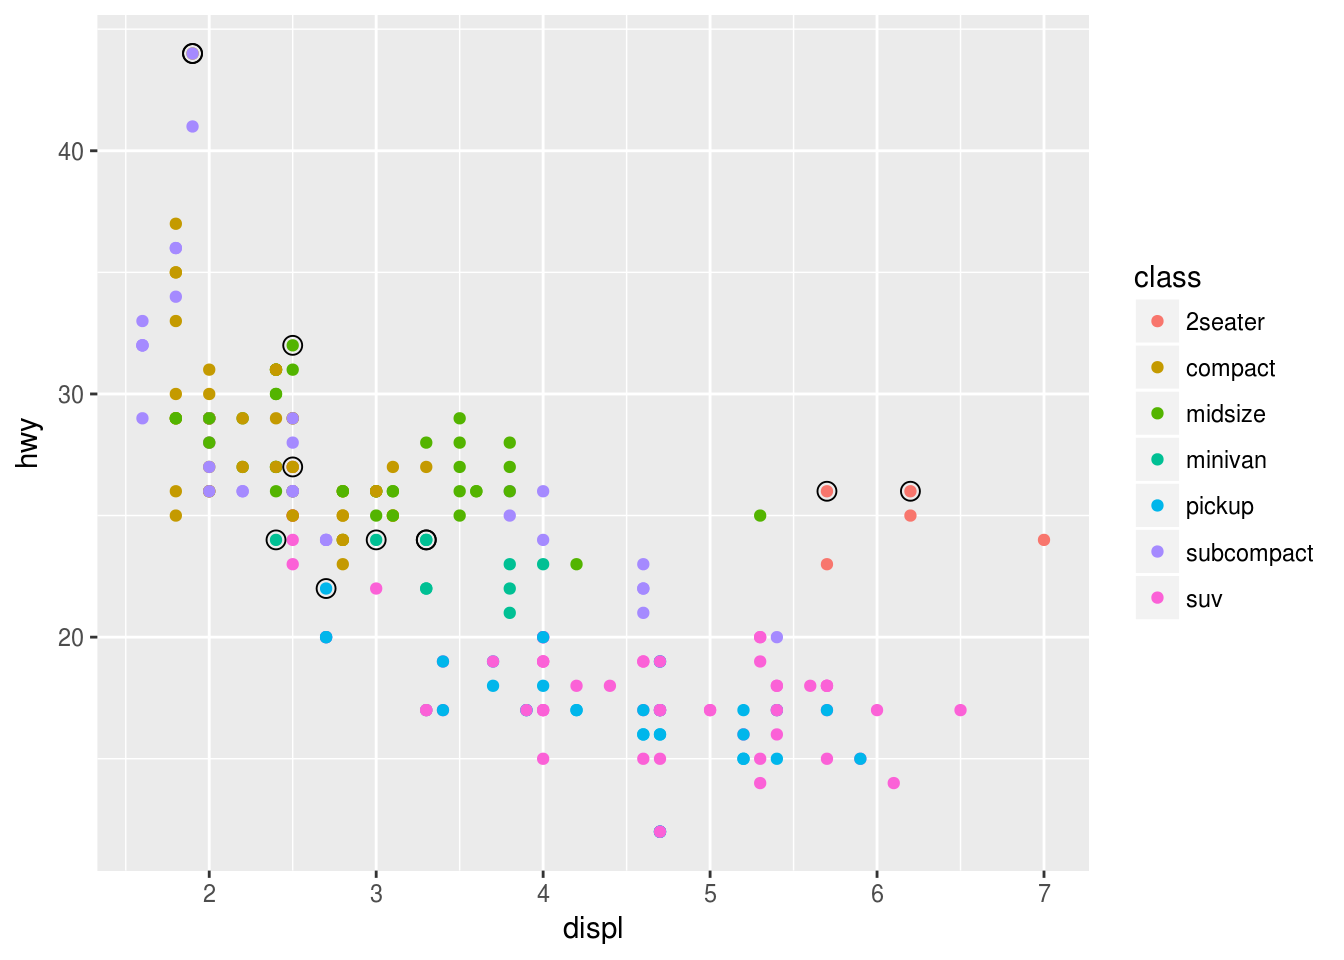
\includegraphics{main_files/figure-latex/unnamed-chunk-179-1.pdf}

\subsection{Kahe muutuja
koos-varieerumine}\label{kahe-muutuja-koos-varieerumine}

\begin{Shaded}
\begin{Highlighting}[]
\KeywordTok{ggplot}\NormalTok{(}\DataTypeTok{data =}\NormalTok{ diamonds, }\KeywordTok{aes}\NormalTok{(}\DataTypeTok{x =}\NormalTok{ depth, }\DataTypeTok{y =}\NormalTok{ price)) }\OperatorTok{+}
\StringTok{  }\KeywordTok{geom_point}\NormalTok{(}\DataTypeTok{size=}\FloatTok{0.1}\NormalTok{, }\DataTypeTok{alpha=}\FloatTok{0.1}\NormalTok{) }\OperatorTok{+}
\StringTok{  }\KeywordTok{geom_density2d}\NormalTok{()}
\end{Highlighting}
\end{Shaded}

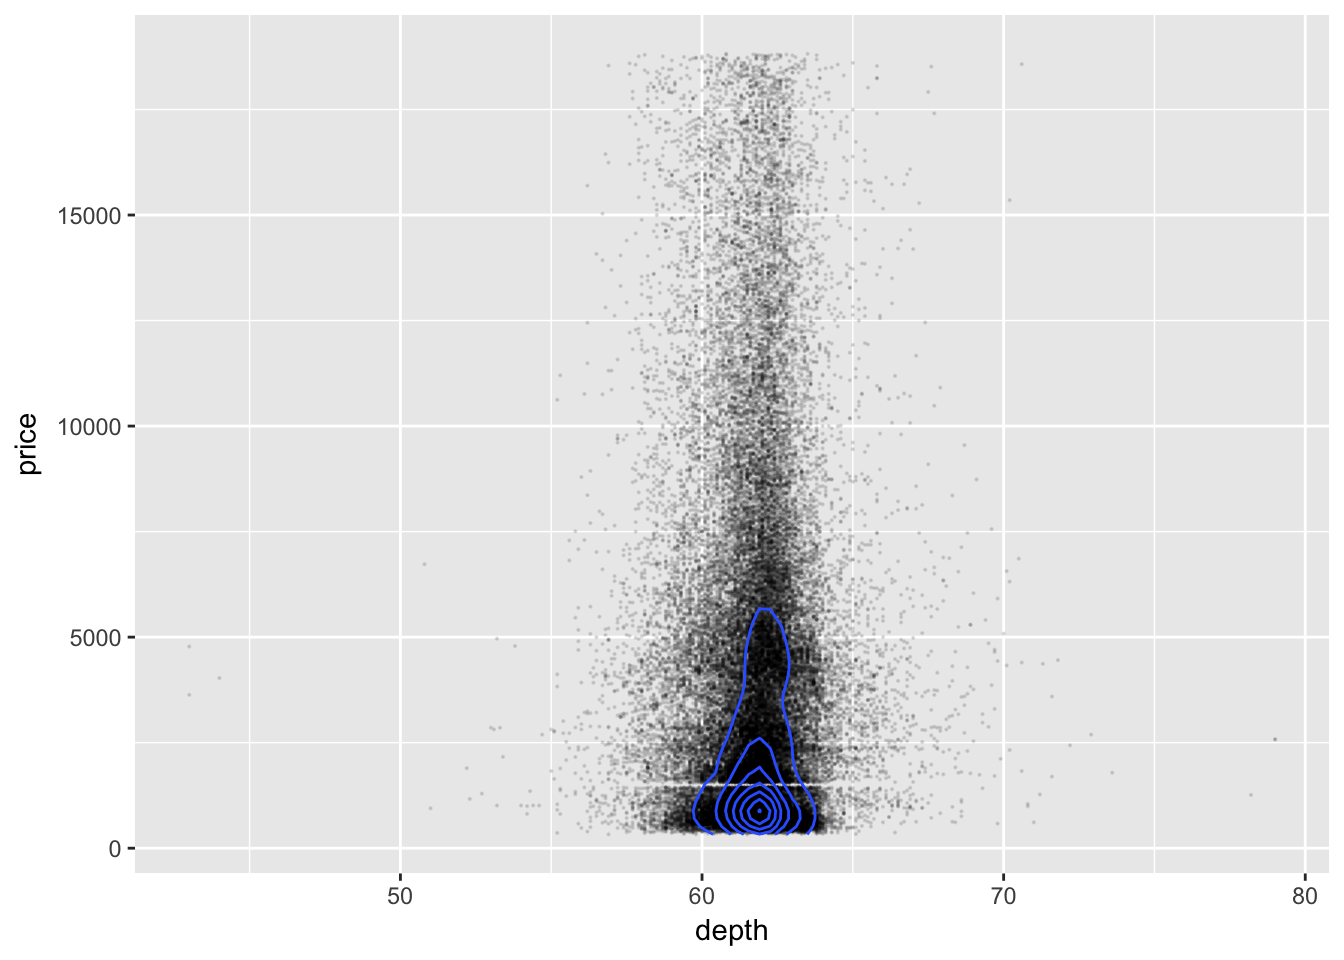
\includegraphics{main_files/figure-latex/unnamed-chunk-180-1.pdf}

Fit a linear model and plot the dots and model:

\begin{Shaded}
\begin{Highlighting}[]
\KeywordTok{ggplot}\NormalTok{(}\DataTypeTok{data=}\NormalTok{iris, }\KeywordTok{aes}\NormalTok{(Sepal.Width, Petal.Width))}\OperatorTok{+}
\StringTok{  }\KeywordTok{geom_point}\NormalTok{()}\OperatorTok{+}
\StringTok{  }\KeywordTok{geom_smooth}\NormalTok{(}\DataTypeTok{method=}\StringTok{"lm"}\NormalTok{, }\DataTypeTok{color=}\StringTok{"red"}\NormalTok{) }
\end{Highlighting}
\end{Shaded}

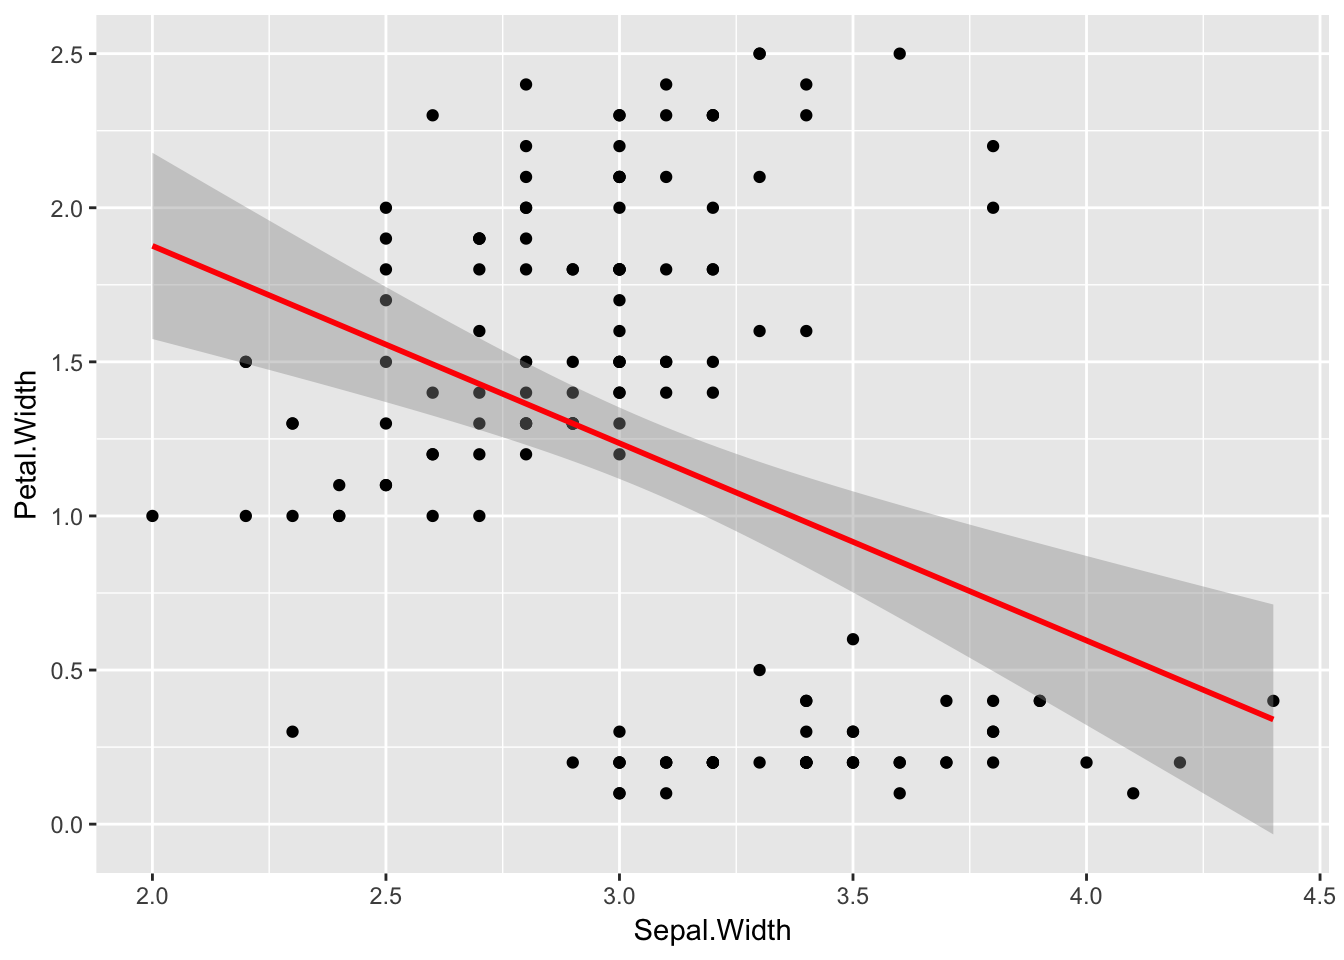
\includegraphics{main_files/figure-latex/unnamed-chunk-181-1.pdf}

\section{Joongraafikud}\label{joongraafikud}

Joonetüübid : ``blank'', ``solid'', ``dashed'', ``dotted'', ``dotdash'',
``longdash'', ``twodash''.

\begin{Shaded}
\begin{Highlighting}[]
\NormalTok{df2 <-}\StringTok{ }\KeywordTok{data.frame}\NormalTok{(}\DataTypeTok{sex =} \KeywordTok{rep}\NormalTok{(}\KeywordTok{c}\NormalTok{(}\StringTok{"Female"}\NormalTok{, }\StringTok{"Male"}\NormalTok{), }\DataTypeTok{each=}\DecValTok{3}\NormalTok{),}
                  \DataTypeTok{time=}\KeywordTok{c}\NormalTok{(}\StringTok{"breakfeast"}\NormalTok{, }\StringTok{"Lunch"}\NormalTok{, }\StringTok{"Dinner"}\NormalTok{),}
                  \DataTypeTok{bill=}\KeywordTok{c}\NormalTok{(}\DecValTok{10}\NormalTok{, }\DecValTok{30}\NormalTok{, }\DecValTok{15}\NormalTok{, }\DecValTok{13}\NormalTok{, }\DecValTok{40}\NormalTok{, }\DecValTok{17}\NormalTok{) )}
\CommentTok{# Change line types}
\KeywordTok{ggplot}\NormalTok{(}\DataTypeTok{data=}\NormalTok{df2, }\KeywordTok{aes}\NormalTok{(}\DataTypeTok{x=}\NormalTok{time, }\DataTypeTok{y=}\NormalTok{bill, }\DataTypeTok{group=}\NormalTok{sex)) }\OperatorTok{+}
\StringTok{  }\KeywordTok{geom_line}\NormalTok{(}\DataTypeTok{linetype=}\StringTok{"dashed"}\NormalTok{)}\OperatorTok{+}
\StringTok{  }\KeywordTok{geom_point}\NormalTok{()}
\end{Highlighting}
\end{Shaded}

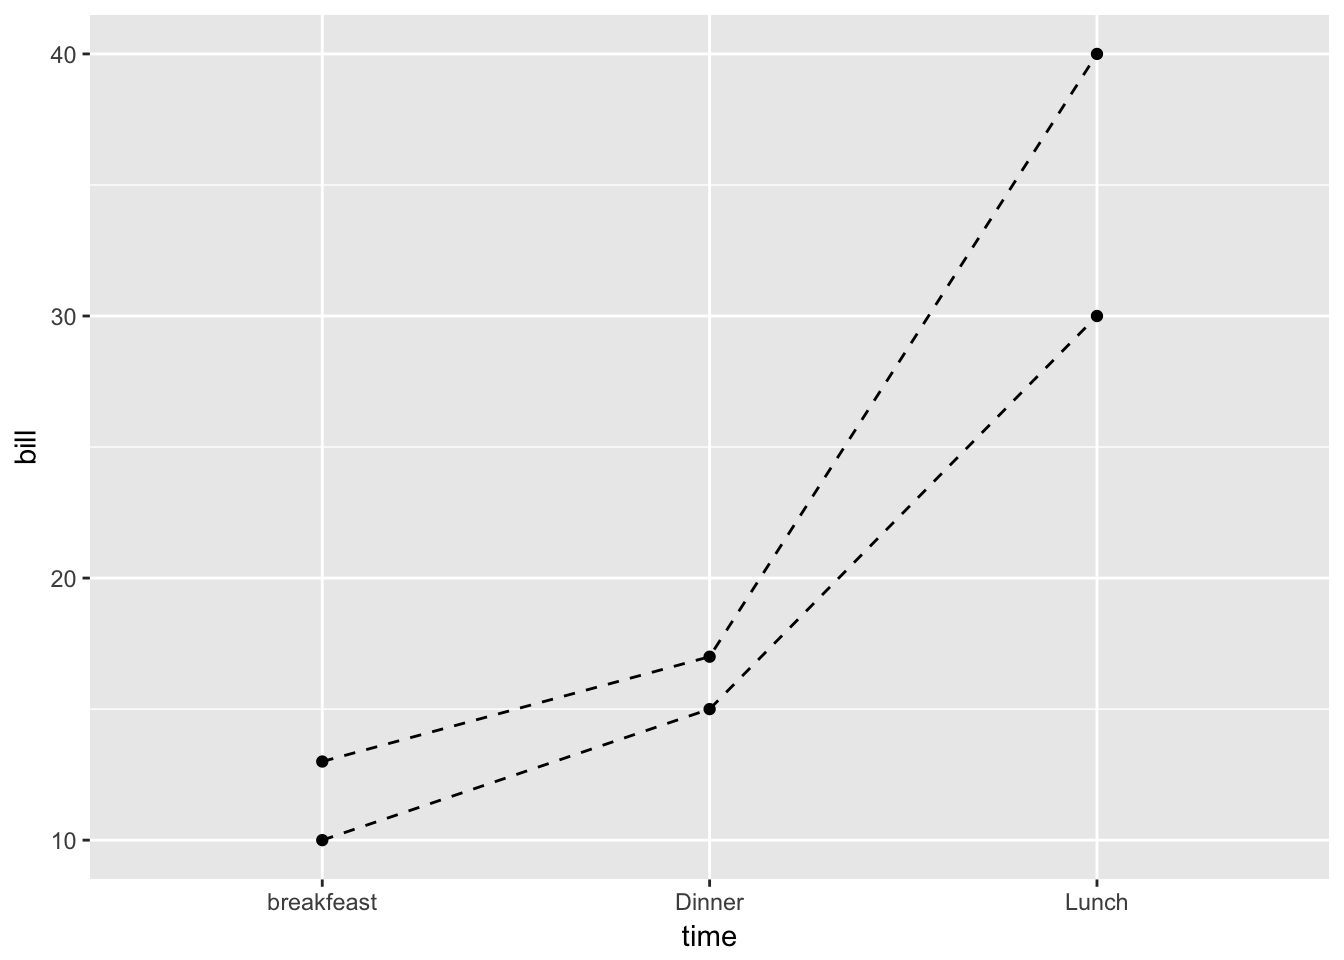
\includegraphics{main_files/figure-latex/unnamed-chunk-182-1.pdf}

\begin{Shaded}
\begin{Highlighting}[]
\CommentTok{# Change line colors and sizes}
\KeywordTok{ggplot}\NormalTok{(}\DataTypeTok{data=}\NormalTok{df2, }\KeywordTok{aes}\NormalTok{(}\DataTypeTok{x=}\NormalTok{time, }\DataTypeTok{y=}\NormalTok{bill, }\DataTypeTok{group=}\NormalTok{sex)) }\OperatorTok{+}
\StringTok{  }\KeywordTok{geom_line}\NormalTok{(}\DataTypeTok{linetype=}\StringTok{"dotted"}\NormalTok{, }\DataTypeTok{color=}\StringTok{"red"}\NormalTok{, }\DataTypeTok{size=}\DecValTok{2}\NormalTok{)}\OperatorTok{+}
\StringTok{  }\KeywordTok{geom_point}\NormalTok{(}\DataTypeTok{color=}\StringTok{"blue"}\NormalTok{, }\DataTypeTok{size=}\DecValTok{3}\NormalTok{)}
\end{Highlighting}
\end{Shaded}

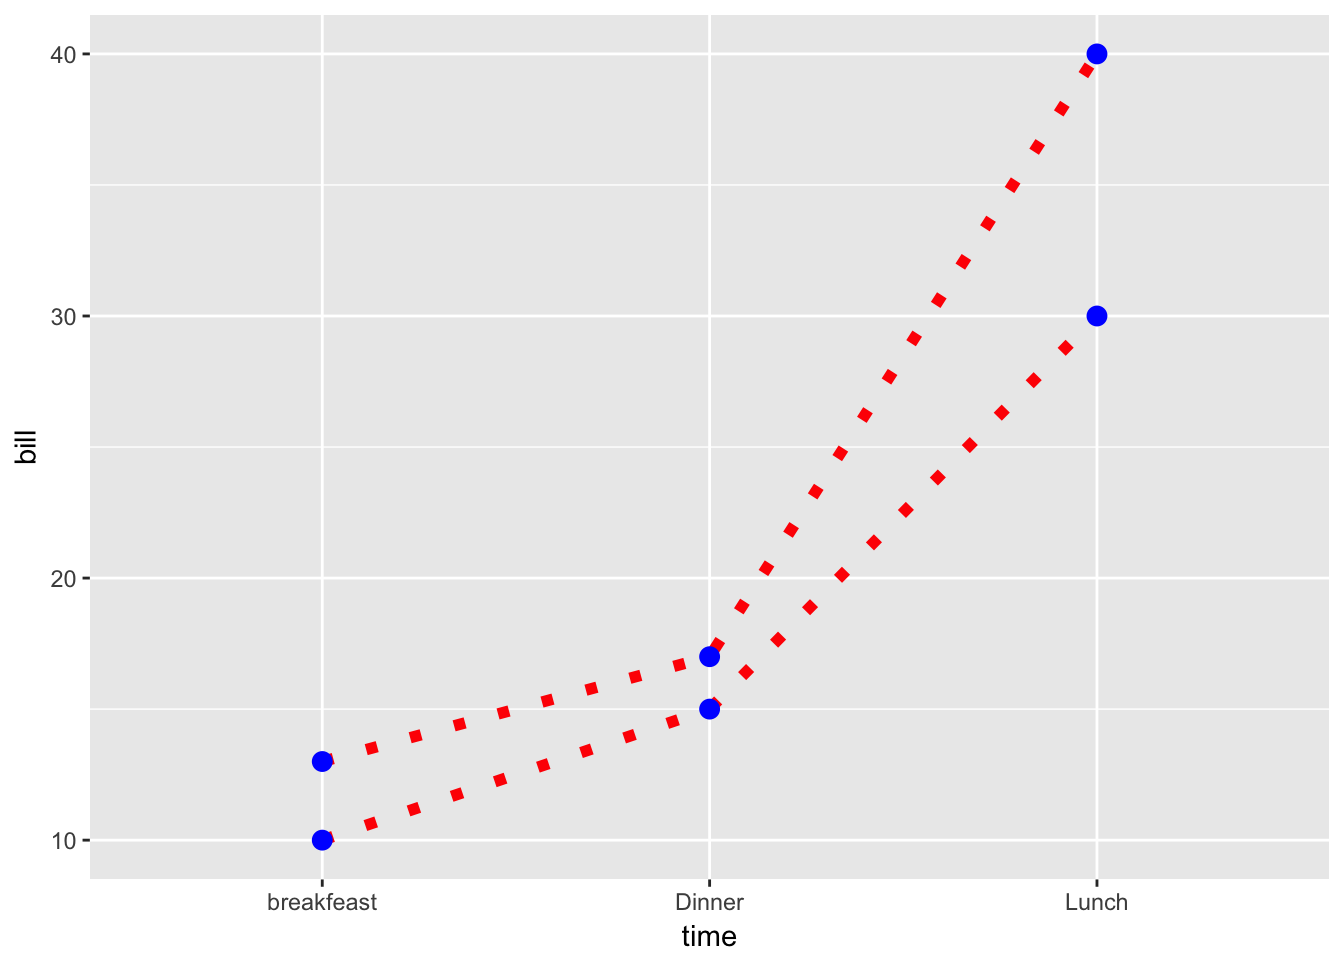
\includegraphics{main_files/figure-latex/unnamed-chunk-182-2.pdf}

Muudab tüüpi automaatselt muutuja sex taseme järgi

\begin{Shaded}
\begin{Highlighting}[]
\CommentTok{# Change line types by groups (sex)}
\KeywordTok{ggplot}\NormalTok{(df2, }\KeywordTok{aes}\NormalTok{(}\DataTypeTok{x=}\NormalTok{time, }\DataTypeTok{y=}\NormalTok{bill, }\DataTypeTok{group=}\NormalTok{sex)) }\OperatorTok{+}
\StringTok{  }\KeywordTok{geom_line}\NormalTok{(}\KeywordTok{aes}\NormalTok{(}\DataTypeTok{linetype=}\NormalTok{sex))}\OperatorTok{+}
\StringTok{  }\KeywordTok{geom_point}\NormalTok{()}\OperatorTok{+}
\StringTok{  }\KeywordTok{theme}\NormalTok{(}\DataTypeTok{legend.position=}\StringTok{"top"}\NormalTok{)}
\end{Highlighting}
\end{Shaded}

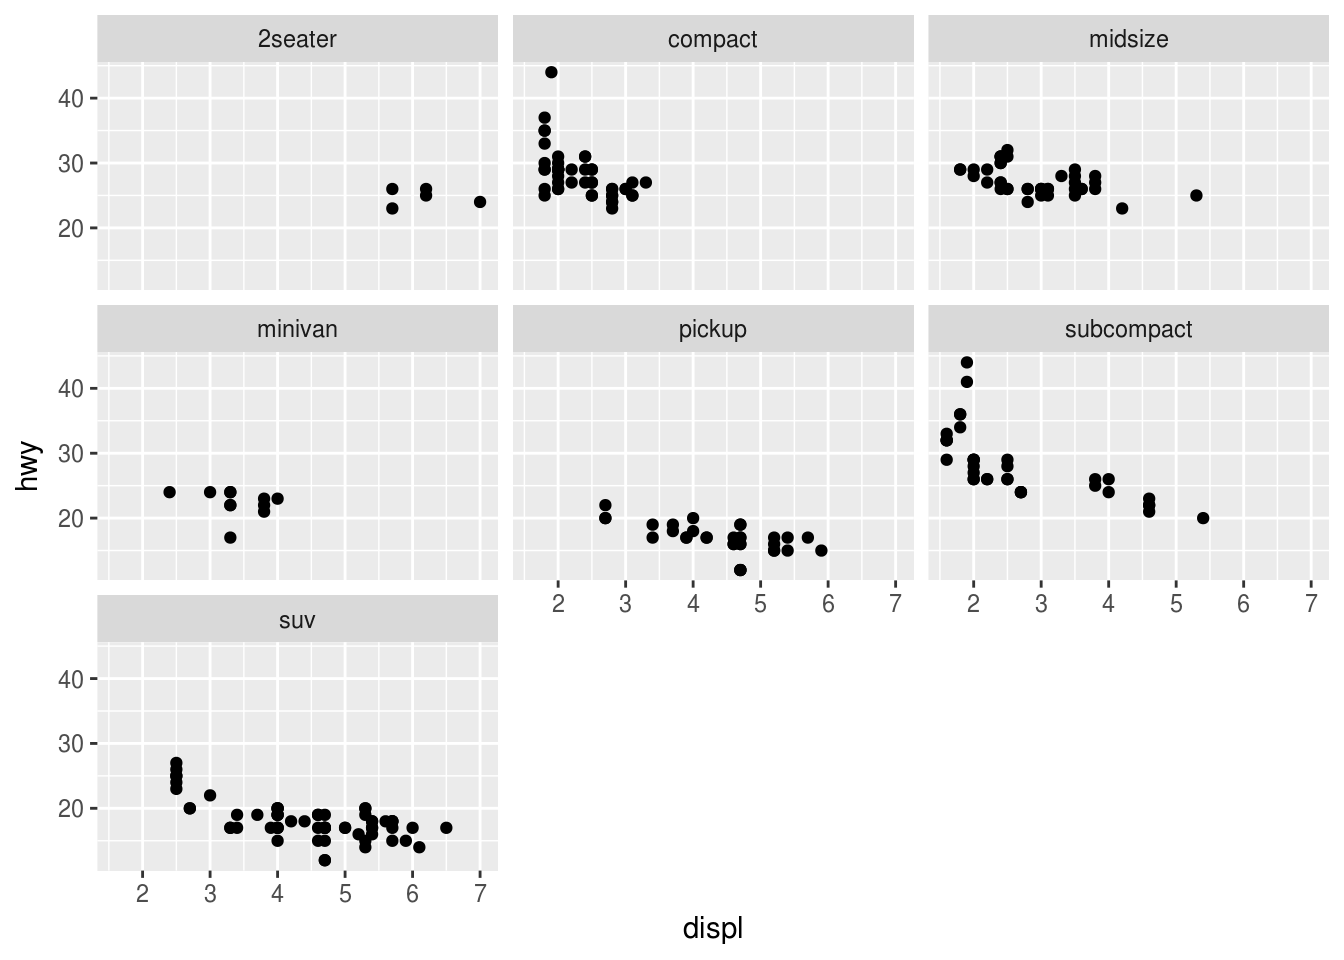
\includegraphics{main_files/figure-latex/unnamed-chunk-183-1.pdf}

\begin{Shaded}
\begin{Highlighting}[]
\CommentTok{# Change line types + colors}
\KeywordTok{ggplot}\NormalTok{(df2, }\KeywordTok{aes}\NormalTok{(}\DataTypeTok{x=}\NormalTok{time, }\DataTypeTok{y=}\NormalTok{bill, }\DataTypeTok{group=}\NormalTok{sex)) }\OperatorTok{+}
\StringTok{  }\KeywordTok{geom_line}\NormalTok{(}\KeywordTok{aes}\NormalTok{(}\DataTypeTok{linetype=}\NormalTok{sex, }\DataTypeTok{color=}\NormalTok{sex))}\OperatorTok{+}
\StringTok{  }\KeywordTok{geom_point}\NormalTok{(}\KeywordTok{aes}\NormalTok{(}\DataTypeTok{color=}\NormalTok{sex))}\OperatorTok{+}
\StringTok{  }\KeywordTok{theme}\NormalTok{(}\DataTypeTok{legend.position=}\StringTok{"top"}\NormalTok{)}
\end{Highlighting}
\end{Shaded}

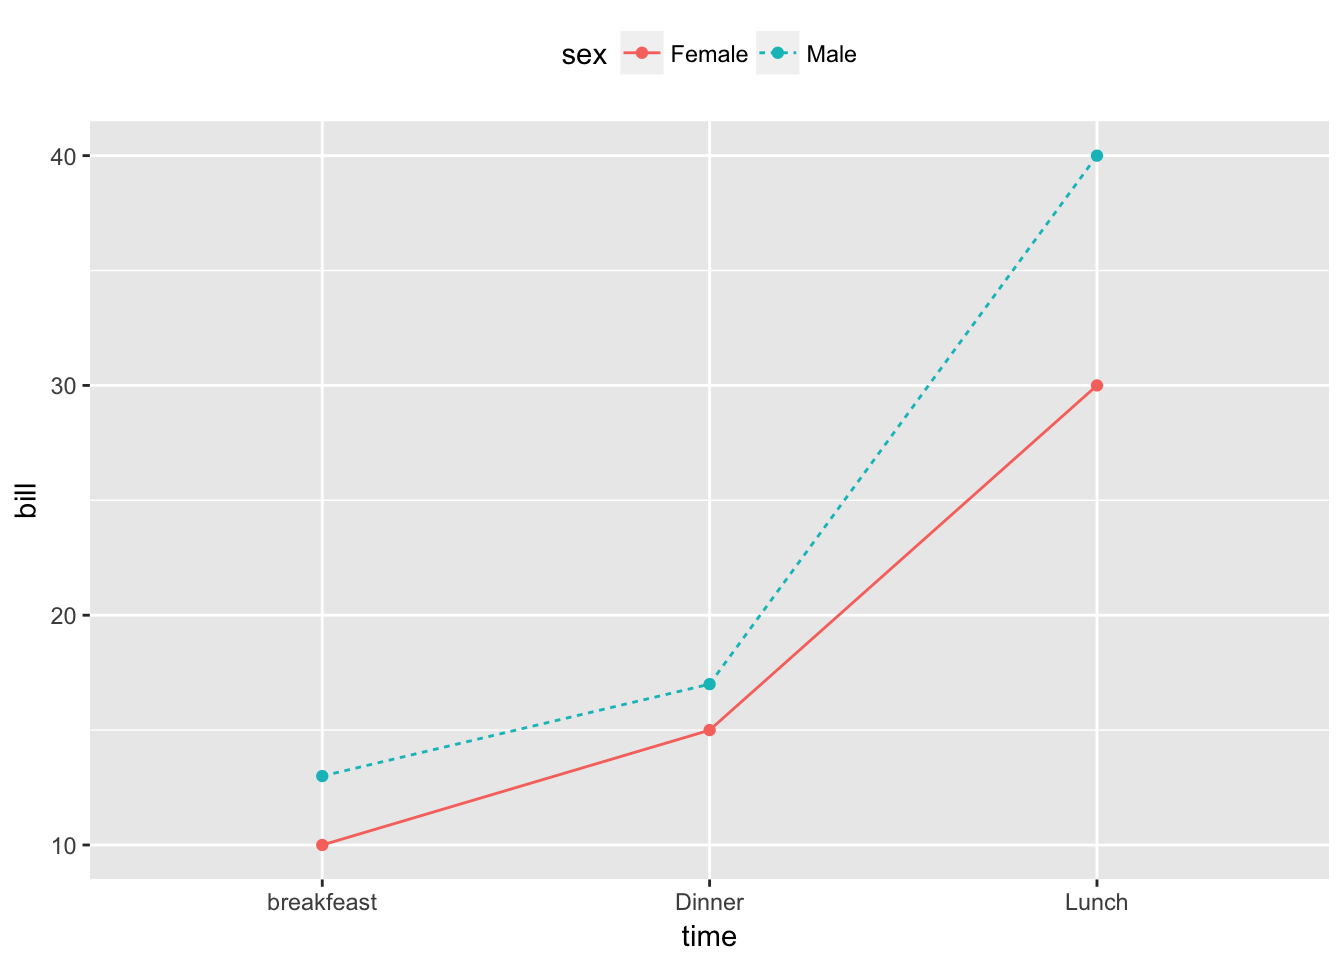
\includegraphics{main_files/figure-latex/unnamed-chunk-183-2.pdf}

Muuda jooni käsitsi:

scale\_linetype\_manual() : joone tüüp

scale\_color\_manual() : joone värv

scale\_size\_manual() : joone laius

\begin{Shaded}
\begin{Highlighting}[]
\CommentTok{# Set line types manually}
\KeywordTok{ggplot}\NormalTok{(df2, }\KeywordTok{aes}\NormalTok{(}\DataTypeTok{x=}\NormalTok{time, }\DataTypeTok{y=}\NormalTok{bill, }\DataTypeTok{group=}\NormalTok{sex)) }\OperatorTok{+}
\StringTok{  }\KeywordTok{geom_line}\NormalTok{(}\KeywordTok{aes}\NormalTok{(}\DataTypeTok{linetype=}\NormalTok{sex))}\OperatorTok{+}
\StringTok{  }\KeywordTok{geom_point}\NormalTok{()}\OperatorTok{+}
\StringTok{  }\KeywordTok{scale_linetype_manual}\NormalTok{(}\DataTypeTok{values=}\KeywordTok{c}\NormalTok{(}\StringTok{"twodash"}\NormalTok{, }\StringTok{"dotted"}\NormalTok{))}\OperatorTok{+}
\StringTok{  }\KeywordTok{theme}\NormalTok{(}\DataTypeTok{legend.position=}\StringTok{"top"}\NormalTok{)}
\end{Highlighting}
\end{Shaded}

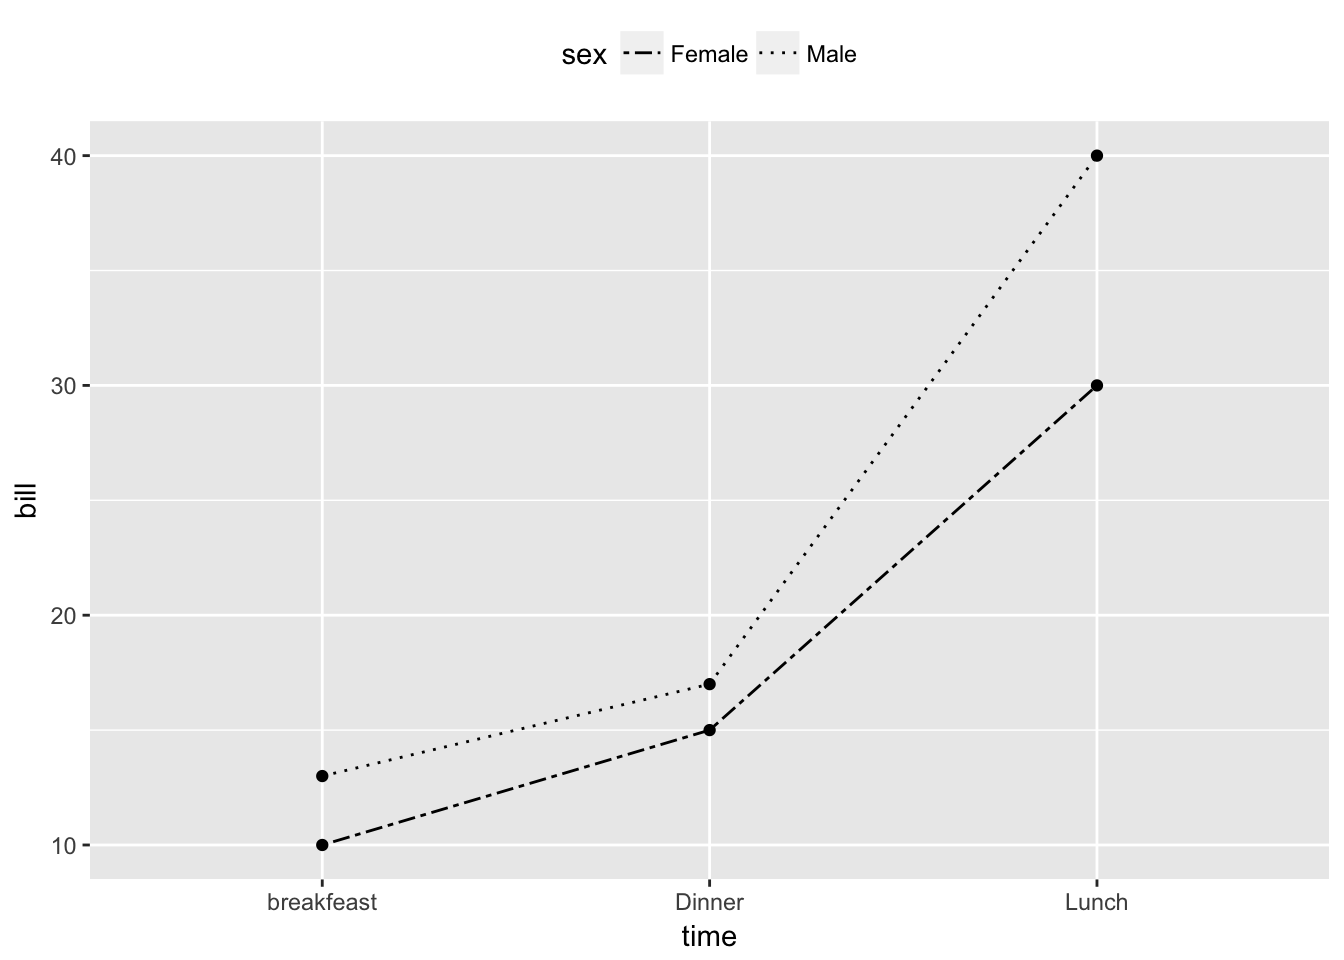
\includegraphics{main_files/figure-latex/unnamed-chunk-184-1.pdf}

\begin{Shaded}
\begin{Highlighting}[]
\CommentTok{# Change line colors and sizes}
\KeywordTok{ggplot}\NormalTok{(df2, }\KeywordTok{aes}\NormalTok{(}\DataTypeTok{x=}\NormalTok{time, }\DataTypeTok{y=}\NormalTok{bill, }\DataTypeTok{group=}\NormalTok{sex)) }\OperatorTok{+}
\StringTok{  }\KeywordTok{geom_line}\NormalTok{(}\KeywordTok{aes}\NormalTok{(}\DataTypeTok{linetype=}\NormalTok{sex, }\DataTypeTok{color=}\NormalTok{sex, }\DataTypeTok{size=}\NormalTok{sex))}\OperatorTok{+}
\StringTok{  }\KeywordTok{geom_point}\NormalTok{()}\OperatorTok{+}
\StringTok{  }\KeywordTok{scale_linetype_manual}\NormalTok{(}\DataTypeTok{values=}\KeywordTok{c}\NormalTok{(}\StringTok{"twodash"}\NormalTok{, }\StringTok{"dotted"}\NormalTok{))}\OperatorTok{+}
\StringTok{  }\KeywordTok{scale_color_manual}\NormalTok{(}\DataTypeTok{values=}\KeywordTok{c}\NormalTok{(}\StringTok{'#999999'}\NormalTok{,}\StringTok{'#E69F00'}\NormalTok{))}\OperatorTok{+}
\StringTok{  }\KeywordTok{scale_size_manual}\NormalTok{(}\DataTypeTok{values=}\KeywordTok{c}\NormalTok{(}\DecValTok{1}\NormalTok{, }\FloatTok{1.5}\NormalTok{))}\OperatorTok{+}
\StringTok{  }\KeywordTok{theme}\NormalTok{(}\DataTypeTok{legend.position=}\StringTok{"top"}\NormalTok{)}
\end{Highlighting}
\end{Shaded}

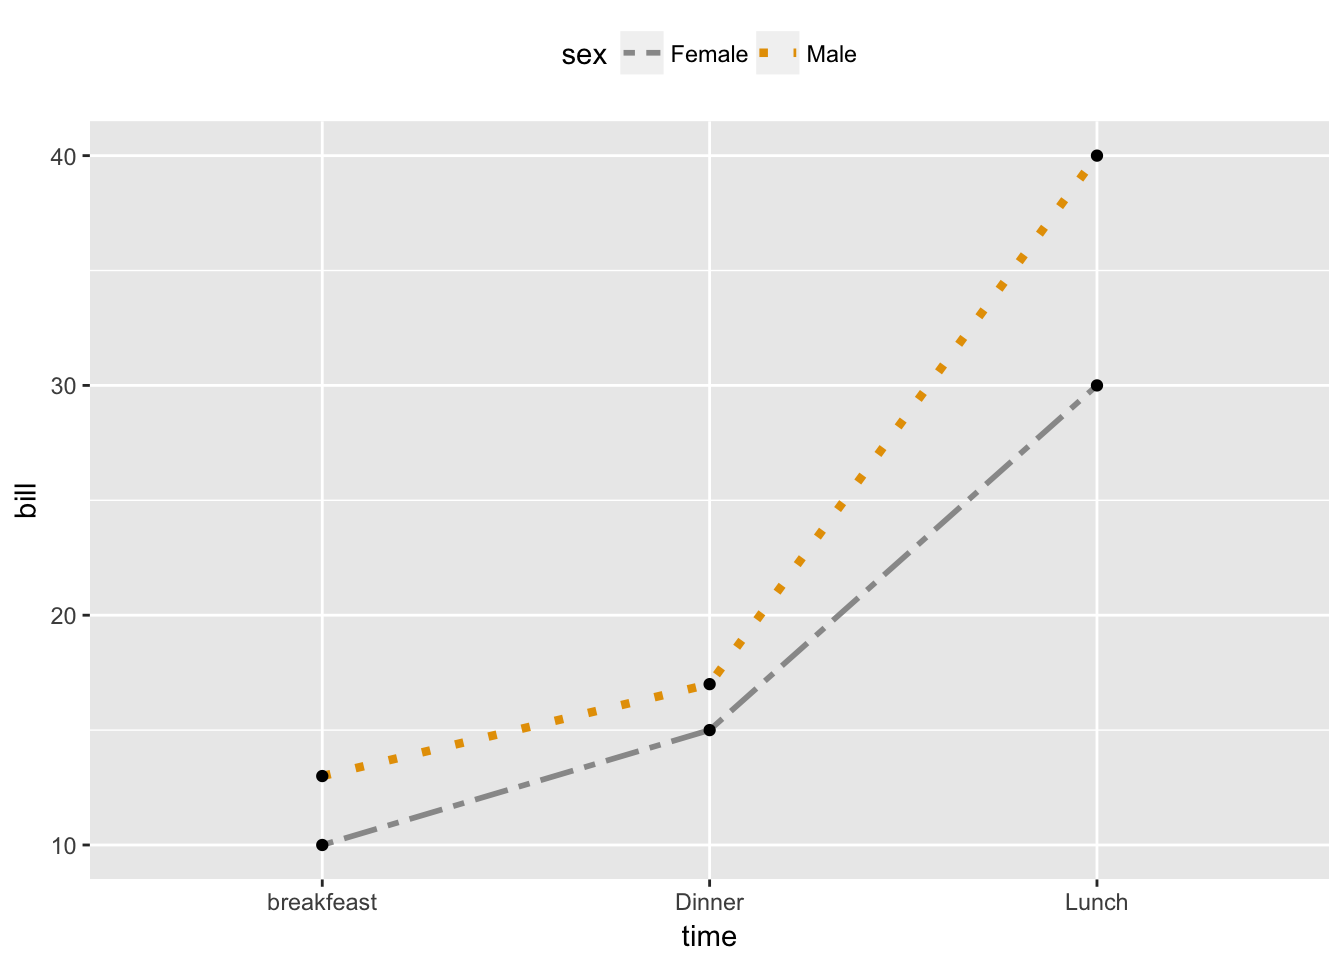
\includegraphics{main_files/figure-latex/unnamed-chunk-184-2.pdf}

\subsubsection{Kokkuvõte:}\label{kokkuvote}

\begin{enumerate}
\def\labelenumi{\alph{enumi}.}
\item
  Andmepunktide plottimine säilitab maksimaalselt andmetes olevat infot
  (nii kasulikku infot kui müra). Aitab leida outliereid (valesti
  sisestatud andmeid, valesti mõõdetud proove jms). Kui valim on väiksem
  kui 20, piisab täiesti üksikute andmepunktide plotist koos mediaaniga.
  Dot-plot ruulib.
\item
  Histogramm -- kõigepealt mõõtskaala ja seejärel andmed jagatakse
  võrdse laiusega binnidesse ja plotitakse binnide kõrgused. Bin, kuhu
  läks 20 andmepunkti on 2X kõrgem kui bin, kuhu läks 10 andmepunkti.
  Samas, bini laius/ulatus mõõteskaalal pole teile ette antud -- ja
  sellest võib sõltuda histogrammi kuju. Seega on soovitav proovida
  erinevaid bini laiusi ja võrrelda saadud histogramme. Histogramm
  sisaldab vähem infot kui dot plot, aga võimaldab paremini tabada
  seaduspärasid \& andmejaotust \& outliereid suurte andmekoguste
  korral.
\item
  Density plot. Silutud versioon histogrammist, mis kaotab infot aga
  toob vahest välja signaali müra arvel. Density plotte on hea kõrvuti
  vaadelda joy ploti abil.
\item
  Box-plot -- sisaldab vähem infot kui histogramm, kuid neid on lihtsam
  kõrvuti võrrelda. Levinuim variant (kuid kahjuks mitte ainus) on Tukey
  box-plot -- mediaan (joon), 50\% IQR (box) ja 1,5x IQR (vuntsid),
  pluss outlierid eraldi punktidena.
\item
  Violin plot -- informatiivsuselt box-ploti ja histogrammi vahepeal --
  sobib paljude jaotuste kõrvuti võrdlemiseks
\item
  Line plot -- kasuta ainult siis kui nii X kui Y teljele on kantud
  pidev väärtus (pikkus, kaal, kontsentratsioon, aeg jms). Ära kasuta,
  kui teljele kantud punktide vahel ei ole looduses mõtet omavaid
  pidevaid väärtusi (näiteks X teljel on katse ja kontroll või erinevad
  valgumutatsioonid, mille aktiivsust on mõõdetud)
\item
  Suhete võrdlemine (pie vs bar)
\item
  Cleveland plot countide jaoks. Kasuta Barplotti ainult siis, kui
  Cleveland plot vm plot mingil põhjusel ei sobi. Barplot võiks olla
  viimane valik.
\end{enumerate}

\begin{quote}
Informatsiooni hulk kahanevalt: iga andmepunkt plotitud (dot plot)
-\textgreater{} histogram -\textgreater{} density plot/violin plot
-\textgreater{} box plot -\textgreater{} bar plot standardhälvetega
-\textgreater{} Cleveland plot (barplot ilma veapiirideta)
\end{quote}

\chapter{Jäta meelde:}\label{jata-meelde}

\begin{enumerate}
\def\labelenumi{\arabic{enumi}.}
\item
  statistika uurib formaalseid mudeleid, mitte teooriaid ega päris
  maailma.
\item
  Statistika jagatakse kahte ossa: kirjeldav ja järeldav (inferential).
\item
  Kirjeldav statistika kirjeldab teie andmeid summaarsete statistikute
  ning graafiliste meetodite abil.
\item
  Järeldav statistika püüab teie andmete põhjal teha järeldusi
  statistilise populatsiooni kohta, millest need andmed pärinevad
\item
  Statistika põhiline ülesanne on kvantifitseerida ebakindlust, mis
  ümbritseb neid järeldusi.
\end{enumerate}

\section{Sõnastik}\label{sonastik}

\begin{itemize}
\item
  Statistiline populatsioon -- objektide kogum, millele soovime teha
  statistilist üldistust. Näiteks hinnata keskmist ravimi mõju
  patsiendipopulatsioonis. Või Escherichia coli ensüümi X keskmist
  Kcat-i.
\item
  Valim -- need objektid (patsiendid, ensüümiprepid), mida me reaalselt
  mõõdame.
\item
  Juhuvalim -- valim, mille liikmed on populatsioonist valitud
  juhuslikult ja iseseisvalt. See tähendab, et kõigil populatsiooni
  liikmetel (kõikidel patsientidel või kõikidel võimalikel
  ensüümipreparatsioonidel) on võrdne võimalus sattuda valimisse JA, et
  valimisse juba sattunud liikme(te) põhjal ei ole võimalik ennustada
  järgmisena valimisse sattuvat liiget.
\item
  Esinduslik valim -- Valim on esinduslik, kui ta peegeldab hästi
  statistilist populatsiooni. Ka juhuvalim ei pruugi olla esinduslik
  (juhuslikult).
\item
  Statistik -- midagi, mis on täpselt arvutatud valimi põhjal (näiteks
  pikkuste keskmine)
\item
  Parameetri väärtus -- teadmata suurus, mille täpset väärtust me saame
  ainult umbkaudu ennustada aga mitte kunagi täpselt teada. (näiteks
  mudeli intercept, populatsiooni keskmine pikkus; efekti suurus =
  katsegrupi keskmine -- kontrollgrupi keskmine)
\item
  Statistiline mudel -- matemaatiline formaliseering, mis sageli koosneb
  2st osast: determinismlik protsessi-mudel pluss juhuslik
  vea/varieeruvuse-mudel. Protsessi-mudeli näiteks kujutle, et mõõdad
  mitme inimese pikkust (X muutuja) ja kaalu (Y muutuja). Sirge
  võrrandiga Y = a + b * X (kaal = a + b * pikkus) saab anda
  determinismliku lineaarse ennustuse kaalu kohta: kui X (pikkus) muutub
  ühe ühiku (cm) võrra, siis muutub Y (kaal) väärtus keskmiselt b ühiku
  (kg) võrra. Seevastu varieeruvuse-mudel on tõenäosusjaotus (näit
  normaaljaotus). Selle abil modelleeritakse Y-suunalist andmete
  varieeruvust igal X väärtusel (näiteks, milline on 182 cm pikkuste
  inimeste oodatav kaalujaotus). Mudel on seega tõenäosuslik: me saame
  näiteks küsida: millise tõenäosusega kaalub 182 cm pikkune inimene üle
  100 kilo. Mida laiem on varieeruvuse mudeli Y-i suunaline jaotus igal
  X-i väärtusel, seda kehvemini ennustab mudel, millist Y väärtust võime
  konkreetselt oodata mingi X-i väärtuse korral. Lineaarsete mudelite
  eesmärk ei ole siiski mitte niivõrd uute andmete ennustamine (seda
  teevad paremini keerulised mudelid), vaid mudeli struktuurist
  lähtuvalt põhjuslike hüpoteeside püstitamine/kontrollimine (kas
  inimese pikkus võiks otseselt reguleerida/kontrollida tema kaalu?).
  Kuna selline viis teadust teha töötab üksnes lihtsate mudelite korral,
  on enamkasutatud statistilised mudelid taotluslikult lihtsustavad ja
  ei pretendeeri tõelähedusele.
\item
  Tehniline replikatsioon -- sama proovi (patsienti,
  ensüümipreparatsiooni, hiire pesakonna liiget) mõõdetakse mitu korda.
  Mõõdab tehnilist varieeruvust ehk mõõtmisviga. Seda püüame kontrollida
  parandades mõõtmisaparatuuri/protokolle või siis juba andmete tasemel,
  statistilise analüüsiga. Näiteks saame andmeid agregeerida ja arvutada
  keskväärtuse. Kui andmepunkte on piisavalt ja varieeruvus on
  sümmeetriline ümber tõelise populatsiooniväärtuse, siis annab
  keksväärtus meile hea hinnangu parameetri tõelisele väärtusele.
\item
  Bioloogiline replikatsioon -- erinevaid patsiente, ensüümipreppe,
  erinevate hiirepesakondade liikmeid mõõdetakse, igaüht üks kord.
  Eesmärk on mõõta Bioloogilist varieeruvust, mis tuleneb mõõteobjektide
  reaalsetest erinevustest: iga patsient ja iga ensüümimolekul on erinev
  kõigist teistest omasugustest. Bioloogiline varieeruvus on
  teaduslikult huvitav ja seda saab visualiseerida algandmete tasemel
  (mitte keskväärtuse tasemel) näiteks histogrammina. Teaduslikke
  järeldusi tehakse bioloogiliste replikaatide põhjal. Tehnilised
  replikaadid seevastu kalibreerivad mõõtesüsteemi täpsust. Kui te
  uurite soolekepikest E. coli, ei saa te teha formaalset järeldust
  kõigi bakterite kohta. Samamoodi, kui te uurite vaid ühe
  hiirepesakonna/puuri liikmeid, ei saa te teha järeldusi kõikide hiirte
  kohta. Kui teie katseskeem sisaldab nii tehnilisi kui bioloogilisi
  replikaate on lihtsaim viis neid andmeid analüüsida kõigepealt
  keskmistada üle tehniliste replikaatide ning seejärel kasutada saadud
  keskmisi edasistes arvutustes üle bioloogiliste replikaatide (näiteks
  arvutada nende pealt uue keskmise, standardhälve ja/või
  usaldusintervalli). Selline kahe-etapiline arvutuskäik ei ole siiski
  optimaalne. Optimaalne, kuid keerukam, on panna mõlemat tüüpi andmed
  ühte hierarhilisse mudelisse.
\end{itemize}

\subsubsection{Tõenäosuse (P) reeglid on ühised kogu
statistikale:}\label{toenaosuse-p-reeglid-on-uhised-kogu-statistikale}

\begin{itemize}
\tightlist
\item
  P jääb 0 ja 1 vahele; P(A) = 1 tähendab, et sündmus A toimub
  kindlasti.
\item
  kui sündmused A ja B on üksteist välistavad, siis tõenäosus, et toimub
  sündmus A või sündmus B on nende kahe sündmuse tõenäosuste summa ---
  P(A v B) = P(A) + P(B).
\item
  Kui A ja B ei ole üksteist välistavad, siis P(A v B) = P(A) + P(B) --
  P(A \& B).
\item
  kui A ja B on üksteisest sõltumatud (A toimumise järgi ei saa
  ennustada B toimumist ja vastupidi) siis tõenäosus, et toimuvad
  mõlemad sündmused on nende sündmuste tõenäosuste korrutis ---- P(A \&
  B) = P(A) x P(B).
\item
  Kui B on loogiliselt A alamosa, siis P(B) \textless{} P(A)
\item
  P(A \textbar{} B) ---- tinglik tõenäosus. Sündmuse A tõenäosus, juhul
  kui peaks toimuma sündmus B. P(vihm \textbar{} pilves ilm) ei ole
  sama, mis P(pilves ilm \textbar{} vihm).
\item
  Juhul kui P(B)\textgreater{}0, siis P(A \textbar{} B) = P(A \& B)/P(B)
  ehk
\item
  P(A \textbar{} B) = P(A) x P(B \textbar{} A)/P(B) ---- Bayesi teoreem.
\end{itemize}

Kuigi kõik statistikud lähtuvad tõenäosustega töötamisel täpselt
samadest matemaatilistest reeglitest, tõlgendavad erinevad koolkonnad
saadud numbreid erinevalt. Kaks põhilist koolkonda on sageduslikud
statistikud ja Bayesiaanid.

\begin{itemize}
\item
  Tõenäosus, sageduslik tõlgendus -- pikaajaline sündmuste suhteline
  sagedus. Näiteks 6-te sagedus paljudel täringuvisetel. Sageduslik
  tõenäosus on teatud tüüpi andmete sagedus, tingimusel et nullhüpotees
  (H0) kehtib; ehk P(andmed \textbar{} H0). Nullhüpotees ütleb enamasti,
  et uuritava parameetri (näiteks ravimiefekti suurus) väärtus on null.
  Seega, kui P on väike, ei ole seda tüüpi andmed kooskõlas arvamusega,
  et parameetri väärtus on null (mis aga ei tähenda automaatselt, et sa
  peaksid uskuma, et parameetri väärtus ei ole null).
\item
  Tõenäosus, Bayesi tõlgendus -- usu määr mingisse hüpoteesi. Näiteks
  62\% tõenäosus (et populatsiooni keskmine pikkus \textless{} 180 cm)
  tähendab, et sa oled ratsionaalse olendina nõus kulutama mitte rohkem
  kui 62 senti kihlveo peale, mis võidu korral toob sulle sisse 1 EUR
  (ja 38 senti kasumit). Bayesi tõenäosus omistatakse statistilisele
  hüpoteesile (näiteks, et ravimiefekti suurus jääb vahemikku a kuni b),
  tingimusel, et sul on täpselt need andmed, mis sul on; ehk P(hüpotees
  \textbar{} andmed).
\end{itemize}

\chapter{Järeldav statistika}\label{jareldav-statistika}

\begin{Shaded}
\begin{Highlighting}[]
\KeywordTok{library}\NormalTok{(tidyverse)}
\KeywordTok{library}\NormalTok{(bayesboot)}
\KeywordTok{library}\NormalTok{(boot)}
\KeywordTok{library}\NormalTok{(rethinking) }\CommentTok{#HPDI() and PI(). Requires Stan.}
\CommentTok{#source("R/")}
\end{Highlighting}
\end{Shaded}

\subsection{3.1. Simulatsiooni jõud}\label{simulatsiooni-joud}

Järeldav statistika püüab valimi põhjal teha järeldusi statistilise
populatsiooni kohta, millest see valim pärineb. Sellisel tegevusel on
mõtet ainult siis, kui ühest küljest valim peegeldab populatsiooni ja
teisest küljest valim ei ole sama asi, mis populatsioon. Seega on
statistika abil tehtud järeldused alati rohkem või vähem ebamäärased
ning meil on vaja meetodit selle ebamäärasuse mõõtmiseks. Aga kõigepealt
illustreerime valimi ja populatsiooni erinevust.

\subsection{3.1.1. Valim ei ole sama, mis
populatsioon}\label{valim-ei-ole-sama-mis-populatsioon}

Simuleerimine on lahe sest erinevalt päris maailmast elavad
simulatsioonid mudeli väikses maailmas ning seega teame me täpselt, mida
me teeme ja mida on meil selle tagajärjel oodata. Simulatsioonidega
saame me hõlpsalt kontrollida, kas ja kuidas meie mudelid töötavad ning
genereerida olukordi (parameetrite väärtuste kombinatsioone), mida päris
maailmas kunagi ette ei tule. Selles mõttes on mudelid korraga nii
väiksemad kui suuremad kui päris maailm.

Alustuseks simuleerime juhuvalimi n=3 lõpmata suurest normaaljaotusega
populatsioonist, mille keskmine on 100 ja sd on 20. Päris elus on
korraliku juhuvalimi tõmbamine tehniliselt tõsine ettevõtmine ja, mis
veelgi olulisem, me ei tea kunagi, milline on populatsiooni tõeline
jaotus, keskmine ja sd. Elagu simulatsioon!

\begin{Shaded}
\begin{Highlighting}[]
\KeywordTok{set.seed}\NormalTok{(}\DecValTok{1}\NormalTok{) }\CommentTok{#makes random number generation reproducible}
\NormalTok{(Sample <-}\StringTok{ }\KeywordTok{rnorm}\NormalTok{(}\DataTypeTok{n =} \DecValTok{3}\NormalTok{, }\DataTypeTok{mean =} \DecValTok{100}\NormalTok{, }\DataTypeTok{sd =} \DecValTok{20}\NormalTok{)) }\CommentTok{#extra parentheses work as print()}
\end{Highlighting}
\end{Shaded}

\begin{verbatim}
## [1]  87.47092 103.67287  83.28743
\end{verbatim}

\begin{Shaded}
\begin{Highlighting}[]
\KeywordTok{mean}\NormalTok{(Sample)}
\end{Highlighting}
\end{Shaded}

\begin{verbatim}
## [1] 91.47707
\end{verbatim}

\begin{Shaded}
\begin{Highlighting}[]
\KeywordTok{sd}\NormalTok{(Sample)}
\end{Highlighting}
\end{Shaded}

\begin{verbatim}
## [1] 10.76701
\end{verbatim}

Nagu näha on meie valimi keskmine 10\% väiksem kui peaks ja valimi sd
lausa kaks korda väiksem kui peaks. Seega peegeldab meie valim halvasti
populatsiooni --- aga me teame seda ainult tänu sellele, et tegu on
simulatsiooniga.

Kui juba simuleerida, siis robinal: tõmbame ühe valimi asemel 10 000,
arvutame seejärel 10 000 keskmist ja sd-d ning vaatame omakorda nende
statistikute jaotusi ja keskväärtusi. Simulatsioon on nagu tselluliit
--- see on nii odav, et igaüks võib seda endale lubada.

Meie lootus on, et kui meil on palju valimeid, millel kõigil on juhuslik
viga, mis neid populatsiooni suhtes ühele või teisele poole kallutab,
siis rohkem on valimeid, mis asuvad tõelisele populatsioonile pigem
lähemal kui kaugemal.

\begin{Shaded}
\begin{Highlighting}[]
\NormalTok{N <-}\StringTok{ }\DecValTok{3}
\NormalTok{N_simulations <-}\StringTok{ }\DecValTok{10000}
\NormalTok{df <-}\StringTok{ }\KeywordTok{tibble}\NormalTok{(}\DataTypeTok{a =} \KeywordTok{rnorm}\NormalTok{(N }\OperatorTok{*}\StringTok{ }\NormalTok{N_simulations, }\DecValTok{100}\NormalTok{, }\DecValTok{20}\NormalTok{), }\DataTypeTok{b =} \KeywordTok{rep}\NormalTok{(}\DecValTok{1}\OperatorTok{:}\NormalTok{N_simulations, }\DataTypeTok{each =}\NormalTok{ N) )}
\NormalTok{Summary <-}\StringTok{  }\NormalTok{df }\OperatorTok\StringTok{ }\KeywordTok{group_by}\NormalTok{(b) }\OperatorTok\StringTok{ }\KeywordTok{summarise}\NormalTok{(}\DataTypeTok{Mean=}\KeywordTok{mean}\NormalTok{(a), }\DataTypeTok{SD=} \KeywordTok{sd}\NormalTok{(a) ) }

\NormalTok{Summary }\OperatorTok\StringTok{ }\KeywordTok{ggplot}\NormalTok{(}\KeywordTok{aes}\NormalTok{(Mean) ) }\OperatorTok{+}\StringTok{ }\KeywordTok{geom_histogram}\NormalTok{()}
\end{Highlighting}
\end{Shaded}

\begin{verbatim}
## `stat_bin()` using `bins = 30`. Pick better value with `binwidth`.
\end{verbatim}

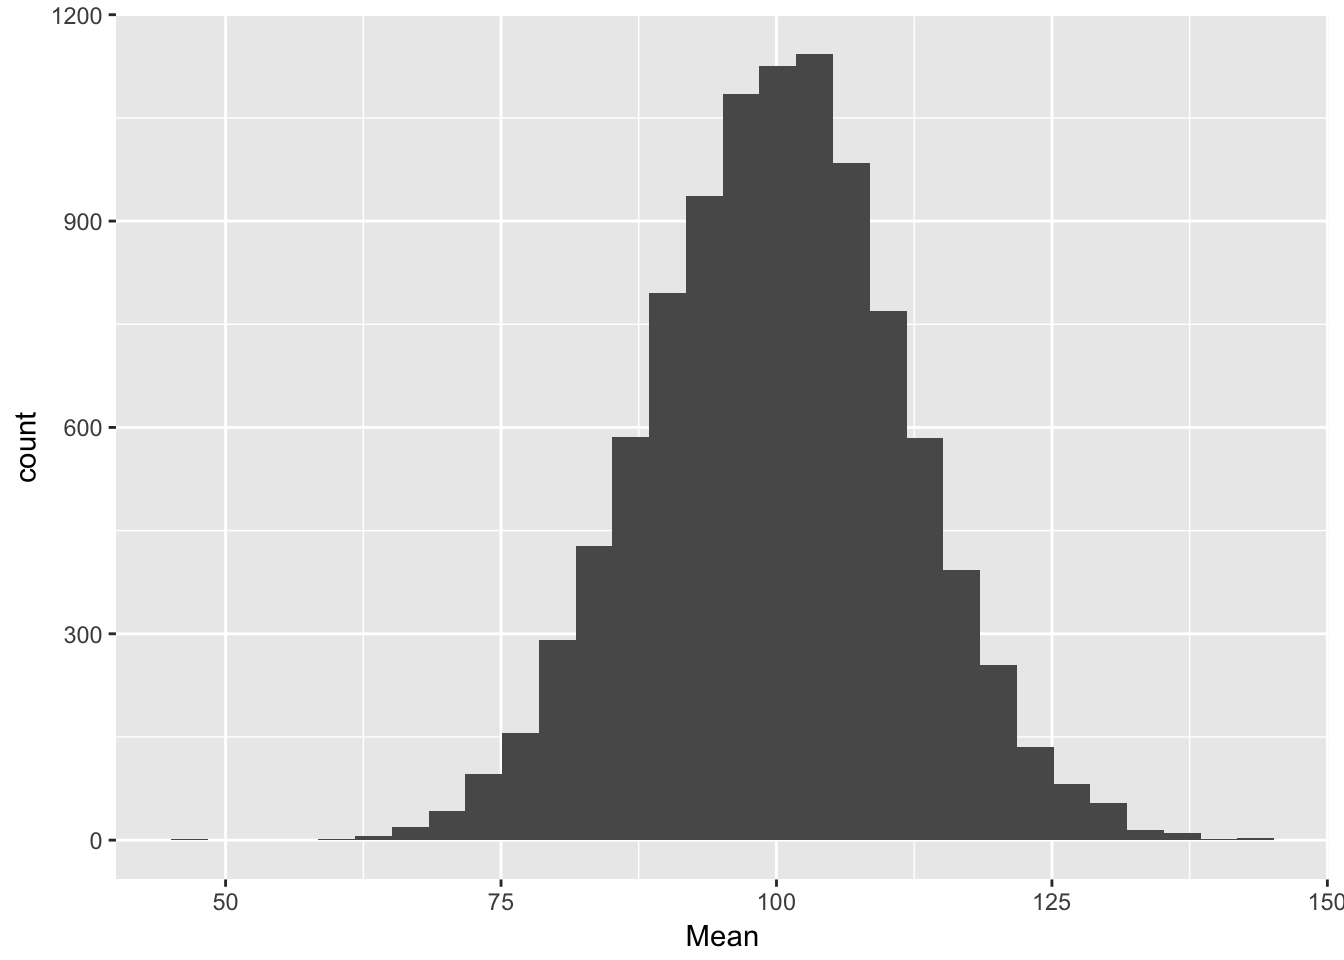
\includegraphics{main_files/figure-latex/unnamed-chunk-187-1.pdf}

\begin{Shaded}
\begin{Highlighting}[]
\KeywordTok{mean}\NormalTok{(Summary}\OperatorTok{$}\NormalTok{Mean) }
\end{Highlighting}
\end{Shaded}

\begin{verbatim}
## [1] 99.98043
\end{verbatim}

\begin{Shaded}
\begin{Highlighting}[]
\KeywordTok{mean}\NormalTok{(Summary}\OperatorTok{$}\NormalTok{SD)}
\end{Highlighting}
\end{Shaded}

\begin{verbatim}
## [1] 17.76452
\end{verbatim}

Oh-hooo. Paljude valimite keskmiste keskmine ennustab väga täpselt
populatsiooni keskmist aga sd-de keskmise keskmine alahindab
populatsiooni sd-d. Valem, millega sd-d arvutatakse tõõtab lihtsalt
kallutatult, kui n on väike (\textless{}10)

Ja nüüd 10 000 SD keskväärtused:

\begin{Shaded}
\begin{Highlighting}[]
\NormalTok{Summary }\OperatorTok\StringTok{ }\KeywordTok{ggplot}\NormalTok{(}\KeywordTok{aes}\NormalTok{(SD)) }\OperatorTok{+}\StringTok{ }\KeywordTok{geom_histogram}\NormalTok{()}
\end{Highlighting}
\end{Shaded}

\begin{verbatim}
## `stat_bin()` using `bins = 30`. Pick better value with `binwidth`.
\end{verbatim}

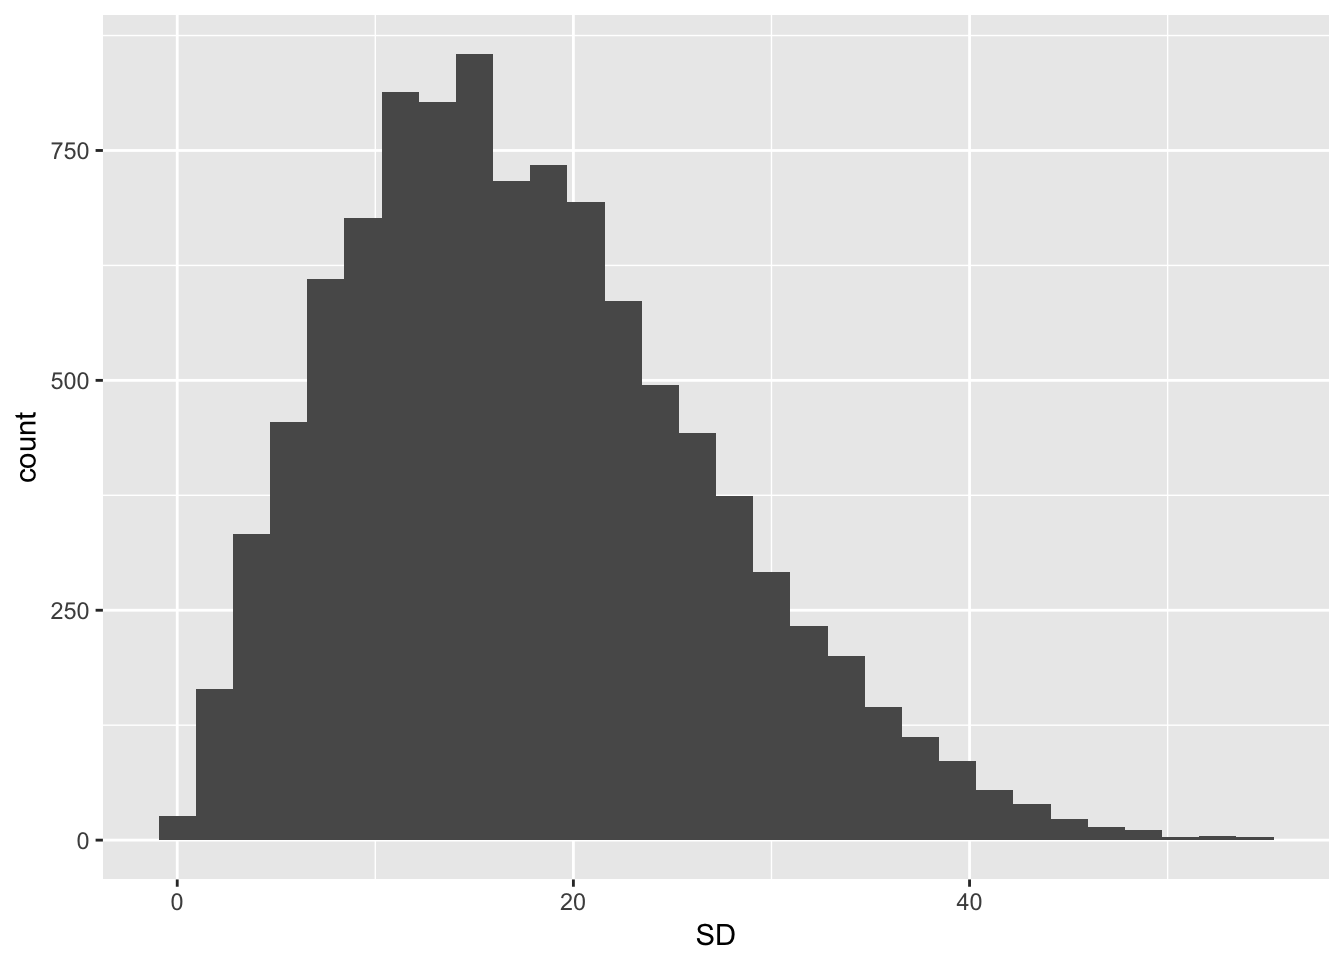
\includegraphics{main_files/figure-latex/unnamed-chunk-189-1.pdf}

\begin{Shaded}
\begin{Highlighting}[]
\NormalTok{mode <-}\StringTok{  }\ControlFlowTok{function}\NormalTok{(x, }\DataTypeTok{adjust=}\DecValTok{1}\NormalTok{) \{}
\NormalTok{  x <-}\StringTok{ }\KeywordTok{na.omit}\NormalTok{(x)}
\NormalTok{  dx <-}\StringTok{ }\KeywordTok{density}\NormalTok{(x, }\DataTypeTok{adjust=}\NormalTok{adjust)}
\NormalTok{y_max <-}\StringTok{ }\NormalTok{dx}\OperatorTok{$}\NormalTok{x[}\KeywordTok{which.max}\NormalTok{(dx}\OperatorTok{$}\NormalTok{y)] }
\NormalTok{y_max}
\NormalTok{\}}
\KeywordTok{mode}\NormalTok{(Summary}\OperatorTok{$}\NormalTok{SD)}
\end{Highlighting}
\end{Shaded}

\begin{verbatim}
## [1] 14.07554
\end{verbatim}

SD-de jaotus on ebasümmeetriline ja mood ehk kõige tõenäolisem valimi sd
väärtus, mida võiksime oodata, on u 14, samal ajal kui populatsiooni sd
= 20. Lisaks on sd-de jaotusel paks saba, mis tagab, et tesest küljest
pole ka vähetõenäoline, et meie valimi sd populatsiooni sd-d kõvasti üle
hindab.

Arvutame, mitu \% valimite sd-e keskmistest on \textgreater{} 25

\begin{Shaded}
\begin{Highlighting}[]
\KeywordTok{sum}\NormalTok{(Summary}\OperatorTok{$}\NormalTok{SD}\OperatorTok{>}\DecValTok{25}\NormalTok{)}\OperatorTok{/}\DecValTok{10000}
\end{Highlighting}
\end{Shaded}

\begin{verbatim}
## [1] 0.2114
\end{verbatim}

Me saame \textgreater{}20\% tõenäosusega pahasti ülehinnatud SD.

\begin{Shaded}
\begin{Highlighting}[]
\KeywordTok{sum}\NormalTok{(Summary}\OperatorTok{$}\NormalTok{SD}\OperatorTok{<}\DecValTok{15}\NormalTok{)}\OperatorTok{/}\DecValTok{10000}
\end{Highlighting}
\end{Shaded}

\begin{verbatim}
## [1] 0.4344
\end{verbatim}

Ja me saame \textgreater{}40\% tõenäosusega pahasti alahinnatud sd.
Selline on väikeste valimite traagika. (Jooksuta sama simulatsiooni n =
100 korral.)

Aga vähemalt populatsiooni keskmise saame me palju valimeid tõmmates
ilusasti kätte --- ka väga väikeste valimitega.

Kahjuks pole meil ei vahendeid ega kannatust 10 000 valimi loodusest
kogumiseks. Enamasti on meil üksainus valim. Õnneks pole sellest väga
hullu sest meil on olemas analoogne meetod, mis töötab üsna hästi ka ühe
valimiga. Seda kutsutakse \emph{bootstrappimiseks} ja selle võttis
esimesena kasutusele parun von Münchausen. Too jutukas parun nimelt
suutis end soomülkast iseenda patsi pidi välja tõmmata, mis ongi
bootstrappimise põhimõte.

\subsection{3.1.2. Bootstrappimine}\label{bootstrappimine}

\begin{quote}
Populatsioon on valimile, mis valim on bootstrappitud valimile.
\end{quote}

Nüüd alustame ühestainsast empiirilisest valimist ja genereerime sellest
10 000 virtuaalset valimit. Selleks tõmbame me oma valimist virtuaalselt
10 000 uut juhuvalimit (bootstrap valimit), igaüks neist sama suur kui
algne valim. Trikk seisneb selles, et bootstrap valimite tõmbamine käib
asendusega, st iga empiirilise valimi element, mis bootstrap valimisse
tõmmatakse, pannakse kohe ka algsesse valimisse tagasi. Seega saab seda
elementi kohe uuesti samasse bootstrap valimisse tõmmata (kui juhus nii
tahab). Seega sisaldab tüüpiline bootstrap valim osasid algse valimi
numbreid mitmes korduses ja teisi üldse mitte. Bootstrap valimid
plotitakse sama moodi nagu me ennist tegime oma valimitega lõpmatust
populatsioonist. Ainsad erinevused on, et bootstrapis on piiratud algse
andmekogu suurus, millest valimeid tõmmatakse ning, et iga bootstrapi
valim on sama suur kui algne andmekogu.

Bootstrap empiirilisele valimile suurusega n töötab nii:

\begin{enumerate}
\def\labelenumi{\arabic{enumi})}
\tightlist
\item
  tõmba empiirilisest valimist k uut virtuaalset valimit, igaüks
  suurusega n
\item
  arvuta keskmine, sd või mistahes muu statistik igale bootstrapi
  valimile. Tee seda k korda.
\item
  joonista oma statistiku väärtustest histogramm või density plot
\item
  nende andmete põhjal saab küsida palju toreidaid küsimusi --- vt
  allpool.
\end{enumerate}

Mis on USA presidentide keskmine pikkus? Meil on valim 10 presidendi
pikkusega.

\begin{Shaded}
\begin{Highlighting}[]
\NormalTok{heights <-}\StringTok{ }\KeywordTok{c}\NormalTok{(}\DecValTok{183}\NormalTok{, }\DecValTok{192}\NormalTok{, }\DecValTok{182}\NormalTok{, }\DecValTok{183}\NormalTok{, }\DecValTok{177}\NormalTok{, }\DecValTok{185}\NormalTok{, }\DecValTok{188}\NormalTok{, }\DecValTok{188}\NormalTok{, }\DecValTok{182}\NormalTok{, }\DecValTok{185}\NormalTok{) }\OperatorTok\StringTok{ }\KeywordTok{as_tibble}\NormalTok{(heights) }
\end{Highlighting}
\end{Shaded}

\begin{verbatim}
## Warning in as.data.frame.numeric(value, stringsAsFactors = FALSE, ...):
## 'row.names' is not a character vector of length 10 -- omitting it. Will be
## an error!
\end{verbatim}

\begin{Shaded}
\begin{Highlighting}[]
\NormalTok{n <-}\StringTok{ }\DecValTok{10} \CommentTok{#sample size}
\NormalTok{nr_boot_samples <-}\StringTok{ }\DecValTok{4000} \CommentTok{#the nr of bootstrap samples}
\NormalTok{a <-}\StringTok{ }\KeywordTok{sample_n}\NormalTok{(heights, n }\OperatorTok{*}\StringTok{ }\NormalTok{nr_boot_samples, }\DataTypeTok{replace=}\OtherTok{TRUE}\NormalTok{)  }\CommentTok{#create random sample with replacement}
\NormalTok{a}\OperatorTok{$}\NormalTok{key <-}\StringTok{ }\KeywordTok{rep}\NormalTok{(}\DecValTok{1}\OperatorTok{:}\NormalTok{nr_boot_samples, }\DataTypeTok{each =}\NormalTok{ n) }\CommentTok{#create a column "key" that cuts the sample into slices of size n}
\NormalTok{a1 <-}\StringTok{ }\NormalTok{a }\OperatorTok\StringTok{ }\KeywordTok{group_by}\NormalTok{(key) }\OperatorTok\StringTok{ }\KeywordTok{summarise}\NormalTok{(}\DataTypeTok{Value=} \KeywordTok{mean}\NormalTok{(value)) }\CommentTok{#calculate the mean for each slice of n values}
\KeywordTok{dens}\NormalTok{(a1}\OperatorTok{$}\NormalTok{Value)}
\end{Highlighting}
\end{Shaded}

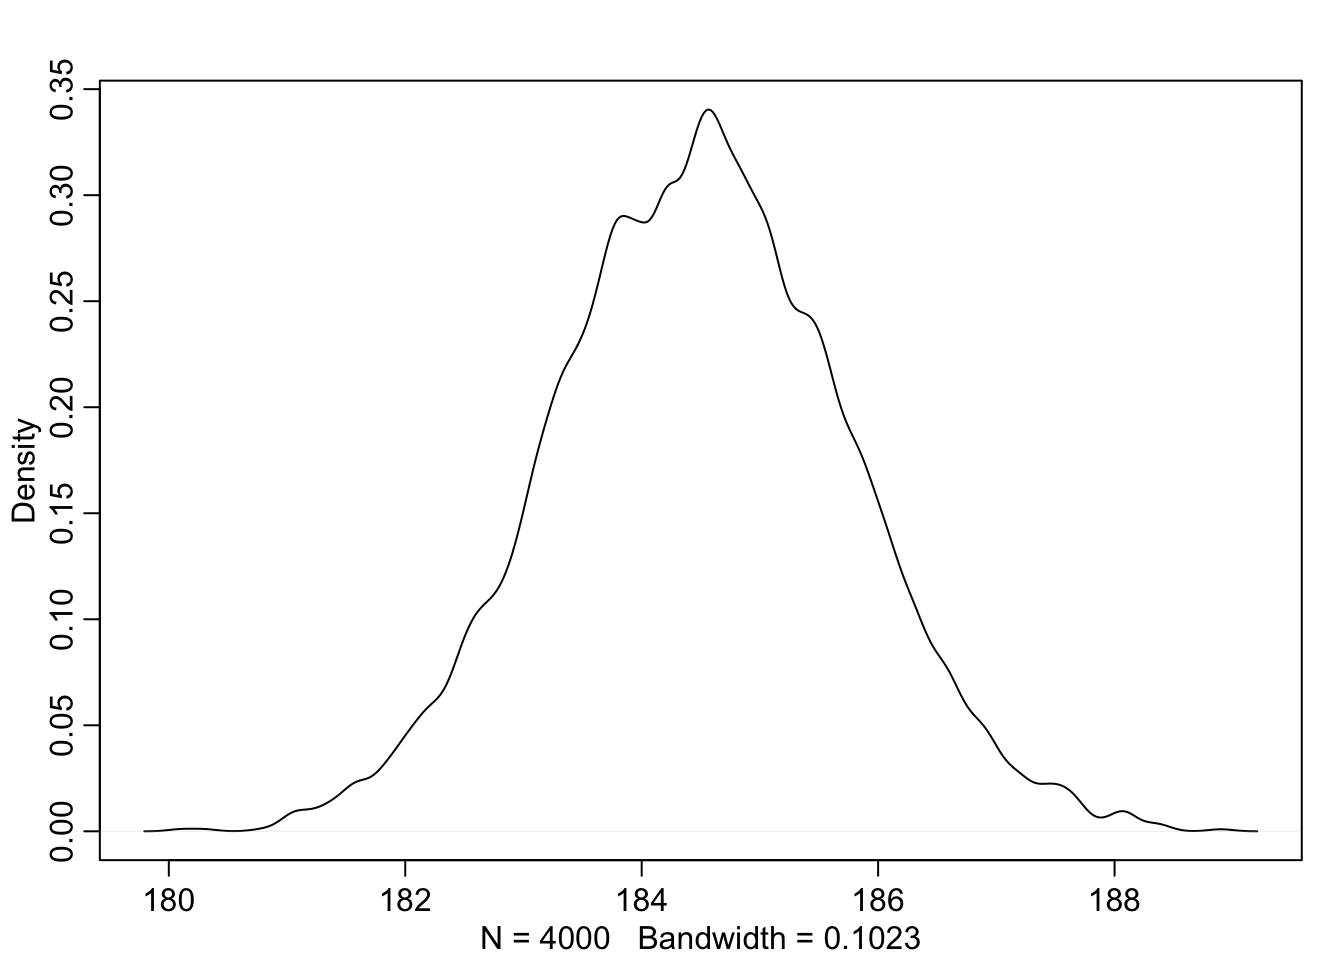
\includegraphics{main_files/figure-latex/unnamed-chunk-193-1.pdf}

Alternatiivne ja aeglasem kood, mis kasutab mosaic::do().

\begin{Shaded}
\begin{Highlighting}[]
\KeywordTok{library}\NormalTok{(mosaic)}
\NormalTok{heights <-}\StringTok{ }\KeywordTok{c}\NormalTok{(}\DecValTok{183}\NormalTok{, }\DecValTok{192}\NormalTok{, }\DecValTok{182}\NormalTok{, }\DecValTok{183}\NormalTok{, }\DecValTok{177}\NormalTok{, }\DecValTok{185}\NormalTok{, }\DecValTok{188}\NormalTok{, }\DecValTok{188}\NormalTok{, }\DecValTok{182}\NormalTok{, }\DecValTok{185}\NormalTok{) }\OperatorTok\StringTok{ }\KeywordTok{as_tibble}\NormalTok{(heights) }
\end{Highlighting}
\end{Shaded}

\begin{verbatim}
## Warning in as.data.frame.numeric(value, stringsAsFactors = FALSE, ...):
## 'row.names' is not a character vector of length 10 -- omitting it. Will be
## an error!
\end{verbatim}

\begin{Shaded}
\begin{Highlighting}[]
\NormalTok{sample_means <-}\StringTok{ }\NormalTok{mosaic}\OperatorTok{::}\KeywordTok{do}\NormalTok{(}\DecValTok{4000}\NormalTok{) }\OperatorTok{*}
\StringTok{    }\NormalTok{(heights }\OperatorTok\StringTok{ }\KeywordTok{sample_n}\NormalTok{(}\DataTypeTok{size =} \DecValTok{10}\NormalTok{, }\DataTypeTok{replace =} \OtherTok{TRUE}\NormalTok{)) }
\end{Highlighting}
\end{Shaded}

\begin{verbatim}
## Using parallel package.
##   * Set seed with set.rseed().
##   * Disable this message with options(`mosaic:parallelMessage` = FALSE)
\end{verbatim}

\begin{Shaded}
\begin{Highlighting}[]
\CommentTok{#võta heigths andmeraamist 10-ne valim (tagasi panekuga) ja tee seda 4000 korda järjest. tulemuseks on tidy tibble, kus on veerg .index, mille järgi saab grupeerida.}

\NormalTok{sample_means1 <-}\StringTok{ }\NormalTok{sample_means }\OperatorTok\StringTok{ }\KeywordTok{group_by}\NormalTok{(.index) }\OperatorTok\StringTok{ }\KeywordTok{summarise}\NormalTok{(}\DataTypeTok{Mean=}\KeywordTok{mean}\NormalTok{(value))}
    
\KeywordTok{ggplot}\NormalTok{(}\DataTypeTok{data =}\NormalTok{ sample_means1, }\KeywordTok{aes}\NormalTok{(}\DataTypeTok{x =}\NormalTok{ Mean)) }\OperatorTok{+}
\StringTok{  }\KeywordTok{geom_histogram}\NormalTok{(}\DataTypeTok{color =} \StringTok{"white"}\NormalTok{, }\DataTypeTok{bins =} \DecValTok{20}\NormalTok{)}
\end{Highlighting}
\end{Shaded}

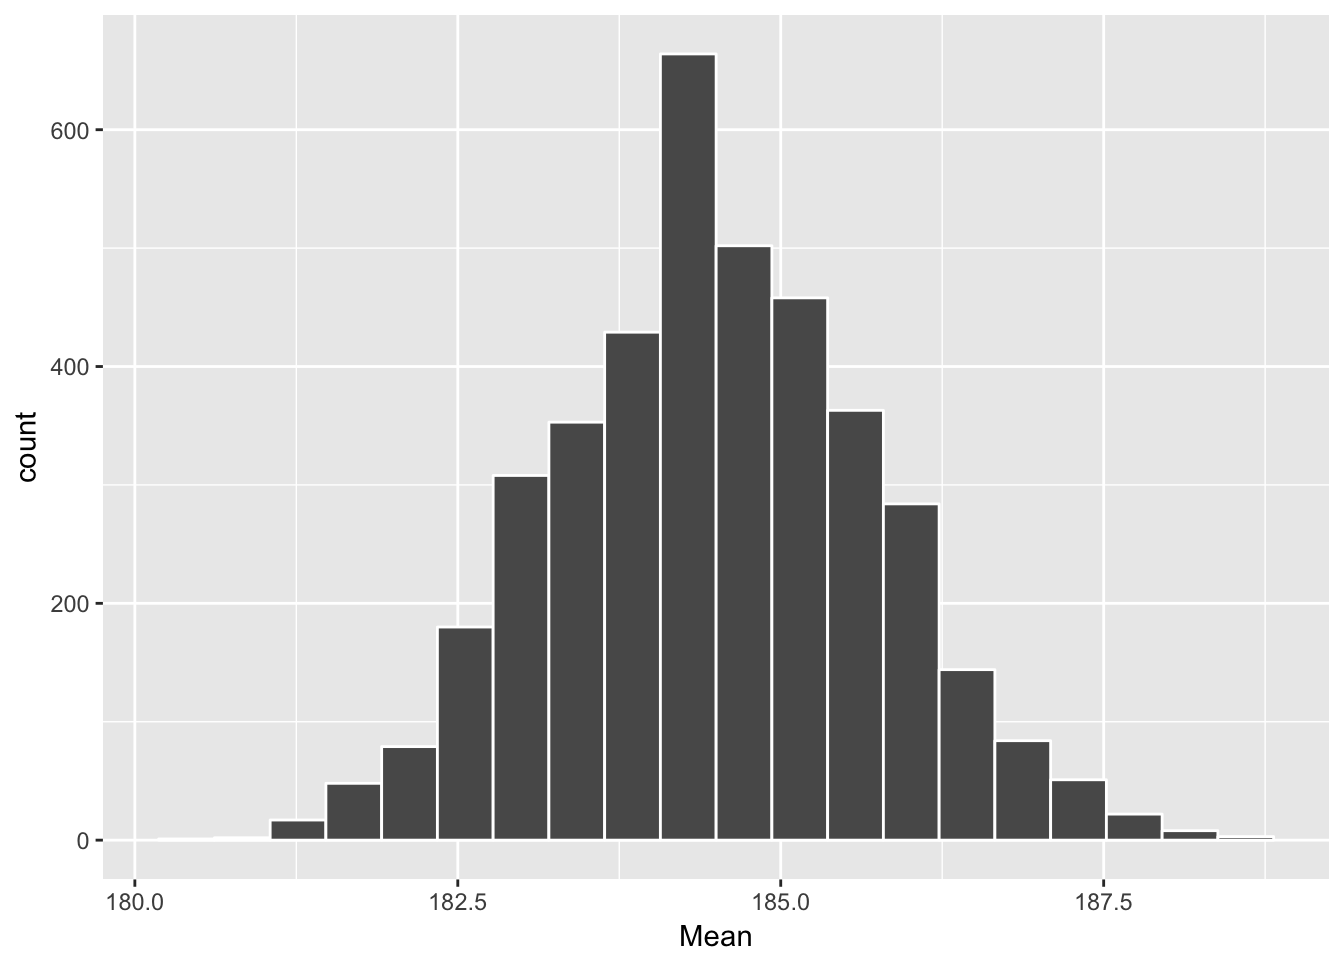
\includegraphics{main_files/figure-latex/unnamed-chunk-194-1.pdf}

Nii saab do() abil 2 veeruga tibble, mille igas veerus on 3 juhuslikku
arvu. NB! kuna ka tidyverse/dplyr sisaldab do() nimelist funktsiooni, on
kasulik seda siin eksplitsiitselt mosaic::do() kaudu esile manada.

\begin{Shaded}
\begin{Highlighting}[]
\NormalTok{mosaic}\OperatorTok{::}\KeywordTok{do}\NormalTok{(}\DecValTok{3}\NormalTok{)}\OperatorTok{*}\StringTok{ }\KeywordTok{rnorm}\NormalTok{(}\DecValTok{2}\NormalTok{)}
\end{Highlighting}
\end{Shaded}

\begin{verbatim}
## Using parallel package.
##   * Set seed with set.rseed().
##   * Disable this message with options(`mosaic:parallelMessage` = FALSE)
\end{verbatim}

\begin{verbatim}
##           V1         V2
## 1 -0.1073985 -0.4952203
## 2  0.6102722  1.0238552
## 3 -1.2747053  0.3952969
\end{verbatim}

Mida selline keskväärtuste jaotus tähendab? Me võime seda vaadelda
posterioorse tõenäosusjaotusena. Selle tõlgenduse kohaselt iseloomustab
see jaotus täpselt meie usku presidentide keskmise pikkuse kohta,
niipalju kui see usk põhineb bootstrappimises kasutatud andmetel.
Senikaua, kui meil pole muid relevantseid andmeid, on kõik, mida me
usume teadvat USA presidentide keskmise pikkuse kohta, peidus selles
jaotuses. Need pikkused, mille kohal jaotus on kõrgem, sisaldavad meie
jaoks tõenäolisemalt tegelikku USA presidentide keskmist pikkust kui
need pikkused, mille kohal posterioorne jaotus on madalam.

Kuidas selle jaotusega edasi töötada? See on lihtne: meil on 4000 arvu
ja me teeme nendega kõike seda, mida parasjagu tahame.

Näiteks me võime arvutada, millisesse pikkuste vahemikku jääb 92\% meie
usust USA presidentide tõelise keskmise pikkuse kohta. See tähendab, et
teades seda vahemikku peaksime olema valmis maksma mitte rohkem kui 92
senti pileti eest, mis juhul kui USA presidentide keskmine pikkus tõesti
jääb sinna vahemikku, toob meile võidu suuruses 1 EUR (ja 8 senti
kasumit). Selline kihlveokontor on muide täiesti respektaabel ja
akadeemiline tõenäosuse tõlgendus; see on paljude arvates lausa parim
tõlgendus, mis meil on.

Miks just 92\% usaldusinterval? Vastus on, et miks mitte? Meil pole
ühtegi universaalset põhjust eelistada üht usaldusvahemiku suurust
teisele. Olgu meil usaldusinteval 90\%, 92\% või 95\% --- tõlgendus on
ikka sama. Nimelt, et me usume, et suure tõenäosusega jääb tegelik
keskväärtus meie poolt arvutatud vahemikku. Mudeli ja maailma erinevused
tingivad niikuinii selle, et konkreetne number ei kandu mudelist üle
pärismaailma. NB! pane tähele, et eelnevalt mainitud kihlveokontor
töötab mudeli maailmas, mitte teie kodu lähedasel hipodroomil.

92\% usaldusintervalli arvutamiseks on kaks meetodit, mis enamasti
annavad vaid veidi erinevaid tulemusi. 1) HPDI --- Highest Density
Probability Interval --- alustab jaotuse tipust (tippudest) ja isoleerib
92\% jaotuse kõrgema(te) osa(de) pindalast 2) PI --- Probability
Interval --- alustab jaotuse servadest ja isoleerib kummagist servast
4\% jaotuse pindalast. See on sama, mis arvutada 4\% ja 96\% kvantiilid

\begin{Shaded}
\begin{Highlighting}[]
\KeywordTok{HPDI}\NormalTok{(a1}\OperatorTok{$}\NormalTok{Value, }\DataTypeTok{prob=}\FloatTok{0.92}\NormalTok{) }\CommentTok{#highest probability density interval - non-symmetric}
\end{Highlighting}
\end{Shaded}

\begin{verbatim}
## |0.92 0.92| 
## 182.3 186.6
\end{verbatim}

\begin{Shaded}
\begin{Highlighting}[]
\KeywordTok{PI}\NormalTok{(a1}\OperatorTok{$}\NormalTok{Value, }\DataTypeTok{prob=}\FloatTok{0.92}\NormalTok{) }\CommentTok{#symmetric method.}
\end{Highlighting}
\end{Shaded}

\begin{verbatim}
##    4%   96% 
## 182.3 186.7
\end{verbatim}

HPDI on üldiselt parem mõõdik kui PI, aga teatud juhtudel on seda raskem
arvutada. Kui HPDI ja PI tugevalt erinevad, on hea mõte piirduda jaotuse
enda avaldamisega --- jaotus ise sisaldab kogu informatsiooni, mis meil
on oma statistiku väärtuse kohta. Intervallid on lihtsalt summaarsed
statistikud andmete kokkuvõtlikuks esitamiseks.

Kui suure tõenäosusega on USA presidentide keskmine pikkus suurem kui
USA populatsiooni meeste keskmine pikkus (178.3 cm mediaan)?

\begin{Shaded}
\begin{Highlighting}[]
\KeywordTok{sum}\NormalTok{(a1}\OperatorTok{$}\NormalTok{Value}\OperatorTok{>}\FloatTok{178.3}\NormalTok{)}\OperatorTok{/}\DecValTok{4000}
\end{Highlighting}
\end{Shaded}

\begin{verbatim}
## [1] 1
\end{verbatim}

\begin{Shaded}
\begin{Highlighting}[]
\KeywordTok{mode}\NormalTok{(a1}\OperatorTok{$}\NormalTok{Value)}
\end{Highlighting}
\end{Shaded}

\begin{verbatim}
## [1] 184.5883
\end{verbatim}

Ligikaudu 100\% tõenäosusega (valimis on 1 mees alla 182 cm, ja tema on
177 cm). Lühikesed jupatsid ei saa Ameerikamaal presidendiks!

Edaspidi kasutame bootstrappimiseks veidi moodsamat meetodit ---
Bayesian bootstrap --- mis töötab veidi paremini väikeste valimite
korral. Aga üldiselt on tulemused sarnased.

\begin{Shaded}
\begin{Highlighting}[]
\KeywordTok{library}\NormalTok{(bayesboot)}
\CommentTok{# Heights of the last ten American presidents in cm (Kennedy to Obama).}
\NormalTok{heights <-}\StringTok{ }\KeywordTok{c}\NormalTok{(}\DecValTok{183}\NormalTok{, }\DecValTok{192}\NormalTok{, }\DecValTok{182}\NormalTok{, }\DecValTok{183}\NormalTok{, }\DecValTok{177}\NormalTok{, }\DecValTok{185}\NormalTok{, }\DecValTok{188}\NormalTok{, }\DecValTok{188}\NormalTok{, }\DecValTok{182}\NormalTok{, }\DecValTok{185}\NormalTok{);}
\NormalTok{b1 <-}\StringTok{ }\KeywordTok{bayesboot}\NormalTok{(heights, mean)}
\KeywordTok{plot}\NormalTok{(b1)}
\end{Highlighting}
\end{Shaded}

\includegraphics{main_files/figure-latex/unnamed-chunk-198-1.pdf}

\begin{Shaded}
\begin{Highlighting}[]
\CommentTok{#summary(b1)}
\CommentTok{#hist(b1)}
\KeywordTok{HPDI}\NormalTok{(b1}\OperatorTok{$}\NormalTok{V1, }\DataTypeTok{prob=}\FloatTok{0.95}\NormalTok{)}
\end{Highlighting}
\end{Shaded}

\begin{verbatim}
##    |0.95    0.95| 
## 182.1153 186.8777
\end{verbatim}

\begin{Shaded}
\begin{Highlighting}[]
\CommentTok{# it's more efficient to use the a weighted statistic (but you can use a normal statistic like mean() or median() as well - as above).}
\NormalTok{b2 <-}\StringTok{ }\KeywordTok{bayesboot}\NormalTok{(heights, weighted.mean, }\DataTypeTok{use.weights =} \OtherTok{TRUE}\NormalTok{)}
\end{Highlighting}
\end{Shaded}

It can also be easily post processed.

\begin{Shaded}
\begin{Highlighting}[]
\CommentTok{# the probability that the mean is > 182 cm.}
\KeywordTok{mean}\NormalTok{( b1[,}\DecValTok{1}\NormalTok{] }\OperatorTok{>}\StringTok{ }\DecValTok{182}\NormalTok{)}
\end{Highlighting}
\end{Shaded}

\begin{verbatim}
## [1] 0.98075
\end{verbatim}

2 keskväärtuse erinevus (keskmine1 - keskmine2):

\begin{Shaded}
\begin{Highlighting}[]
\NormalTok{df <-}\StringTok{ }\KeywordTok{tibble}\NormalTok{(}\DataTypeTok{a=}\KeywordTok{rnorm}\NormalTok{(}\DecValTok{10}\NormalTok{), }\DataTypeTok{b=}\KeywordTok{rnorm}\NormalTok{(}\DecValTok{10}\NormalTok{,}\DecValTok{1}\NormalTok{,}\DecValTok{1}\NormalTok{))}
\NormalTok{m1 <-}\StringTok{ }\KeywordTok{bayesboot}\NormalTok{(df}\OperatorTok{$}\NormalTok{a, mean)}
\NormalTok{m2 <-}\StringTok{ }\KeywordTok{bayesboot}\NormalTok{(df}\OperatorTok{$}\NormalTok{b, mean)}
\NormalTok{m12 <-}\StringTok{ }\KeywordTok{bind_cols}\NormalTok{(m1, m2) }
\NormalTok{m12 <-}\StringTok{ }\NormalTok{m12 }\OperatorTok\StringTok{ }\KeywordTok{mutate}\NormalTok{(}\DataTypeTok{value=}\NormalTok{m12[,}\DecValTok{2}\NormalTok{] }\OperatorTok{-}\StringTok{ }\NormalTok{m12[,}\DecValTok{1}\NormalTok{])}
\KeywordTok{hist}\NormalTok{(m12}\OperatorTok{$}\NormalTok{value)}
\end{Highlighting}
\end{Shaded}

\includegraphics{main_files/figure-latex/unnamed-chunk-201-1.pdf}

\begin{Shaded}
\begin{Highlighting}[]
\KeywordTok{median}\NormalTok{(m12}\OperatorTok{$}\NormalTok{value)}
\end{Highlighting}
\end{Shaded}

\begin{verbatim}
## [1] 1.624235
\end{verbatim}

\begin{Shaded}
\begin{Highlighting}[]
\KeywordTok{mode}\NormalTok{(m12}\OperatorTok{$}\NormalTok{value)}
\end{Highlighting}
\end{Shaded}

\begin{verbatim}
## [1] 1.543269
\end{verbatim}

\begin{Shaded}
\begin{Highlighting}[]
\KeywordTok{HPDI}\NormalTok{(m12}\OperatorTok{$}\NormalTok{value)}
\end{Highlighting}
\end{Shaded}

\begin{verbatim}
##    |0.89    0.89| 
## 1.116852 2.183880
\end{verbatim}

\begin{Shaded}
\begin{Highlighting}[]
\CommentTok{#library(BayesianFirstAid); bayes.t.test(m1, m2) }
\CommentTok{#will give a similar, but fully Bayesian, result}
\CommentTok{#requires JAGS.}
\end{Highlighting}
\end{Shaded}

\textbf{Bayesian bootstrap SD arvutamiseks.}

When use.weights = FALSE it is important that the summary statistics
does not change as a function of sample size. This is the case with the
sample standard deviation, so here we have to implement a function
calculating the population standard deviation.

\begin{Shaded}
\begin{Highlighting}[]
\NormalTok{pop.sd <-}\StringTok{ }\ControlFlowTok{function}\NormalTok{(x) \{}
\NormalTok{  n <-}\StringTok{ }\KeywordTok{length}\NormalTok{(x)}
  \KeywordTok{sd}\NormalTok{(x) }\OperatorTok{*}\StringTok{ }\KeywordTok{sqrt}\NormalTok{( (n }\OperatorTok{-}\StringTok{ }\DecValTok{1}\NormalTok{) }\OperatorTok{/}\StringTok{ }\NormalTok{n)}
\NormalTok{\}}

\NormalTok{b3 <-}\StringTok{ }\KeywordTok{bayesboot}\NormalTok{(heights, pop.sd)}
\KeywordTok{summary}\NormalTok{(b3)}
\end{Highlighting}
\end{Shaded}

\begin{verbatim}
## Bayesian bootstrap
## 
## Number of posterior draws: 4000 
## 
## Summary of the posterior (with 95% Highest Density Intervals):
##  statistic     mean        sd  hdi.low hdi.high
##         V1 3.663116 0.7391744 2.230017 5.031605
## 
## Quantiles:
##  statistic    q2.5%     q25%   median     q75%   q97.5%
##         V1 2.323455 3.121658 3.654356 4.159498 5.158932
## 
## Call:
##  bayesboot(data = heights, statistic = pop.sd)
\end{verbatim}

A Bayesian bootstrap analysis of a correlation coefficient

\begin{Shaded}
\begin{Highlighting}[]
\CommentTok{#Data comparing two methods of measuring blood flow.}
\NormalTok{blood.flow <-}\StringTok{ }\KeywordTok{data.frame}\NormalTok{(}
  \DataTypeTok{dye =} \KeywordTok{c}\NormalTok{(}\FloatTok{1.15}\NormalTok{, }\FloatTok{1.7}\NormalTok{, }\FloatTok{1.42}\NormalTok{, }\FloatTok{1.38}\NormalTok{, }\FloatTok{2.80}\NormalTok{, }\FloatTok{4.7}\NormalTok{, }\FloatTok{4.8}\NormalTok{, }\FloatTok{1.41}\NormalTok{, }\FloatTok{3.9}\NormalTok{),}
  \DataTypeTok{efp =} \KeywordTok{c}\NormalTok{(}\FloatTok{1.38}\NormalTok{, }\FloatTok{1.72}\NormalTok{, }\FloatTok{1.59}\NormalTok{, }\FloatTok{1.47}\NormalTok{, }\FloatTok{1.66}\NormalTok{, }\FloatTok{3.45}\NormalTok{, }\FloatTok{3.87}\NormalTok{, }\FloatTok{1.31}\NormalTok{, }\FloatTok{3.75}\NormalTok{))}

\CommentTok{# Using the weighted correlation (corr) from the boot package.}
\KeywordTok{library}\NormalTok{(boot)}
\NormalTok{b4 <-}\StringTok{ }\KeywordTok{bayesboot}\NormalTok{(blood.flow, corr, }\DataTypeTok{R =} \DecValTok{1000}\NormalTok{, }\DataTypeTok{use.weights =} \OtherTok{TRUE}\NormalTok{)}
\KeywordTok{plot}\NormalTok{(b4)}
\end{Highlighting}
\end{Shaded}

\includegraphics{main_files/figure-latex/unnamed-chunk-203-1.pdf}

A Bayesian bootstrap analysis of lm coefficients

\begin{Shaded}
\begin{Highlighting}[]
\CommentTok{# A custom function that returns the coefficients of}
\CommentTok{# a weighted linear regression on the blood.flow data}
\NormalTok{lm.coefs <-}\StringTok{ }\ControlFlowTok{function}\NormalTok{(d, w) \{}
  \KeywordTok{coef}\NormalTok{( }\KeywordTok{lm}\NormalTok{(efp }\OperatorTok{~}\StringTok{ }\NormalTok{dye, }\DataTypeTok{data =}\NormalTok{ d, }\DataTypeTok{weights =}\NormalTok{ w) )}
\NormalTok{\}}

\NormalTok{b5 <-}\StringTok{ }\KeywordTok{bayesboot}\NormalTok{(blood.flow, lm.coefs, }\DataTypeTok{R =} \DecValTok{1000}\NormalTok{, }\DataTypeTok{use.weights =} \OtherTok{TRUE}\NormalTok{)}
\KeywordTok{plot}\NormalTok{(b5)}
\end{Highlighting}
\end{Shaded}

\includegraphics{main_files/figure-latex/unnamed-chunk-204-1.pdf}

Bootstrappimine on väga hea meetod, mis sõltub väiksemast arvust
eeldustest kui statistikas tavaks. Bootstrap ei eelda, et andmed on
normaaljaotusega või mõne muu matemaatiliselt lihtsa jaotusega. Tema
põhiline eeldus on, et valim peegeldab populatsiooni --- mis ei pruugi
kehtida väikeste valimite korral ja kallutatud (mitte-juhuslike)
valimite korral.

Bootstrappimisel on üks konseptuaalne puudus, mis on eriti tõsine
väikeste valimite korral. Võtame oma näite USA presidentidest. Meie
valimi liikmed on kõik presideerinud viimase 50 aasta jooksul, aga selle
aja jooksul on inimeste keskmine pikkus jõudsalt kasvanud. Kui me tahame
ennustada järgmise 50 aasta keskmist presidentide pikkust, peaksime
selle faktiga arvestama. Aga bootstrap ei jäta meile sellist võimalust.
Vähemalt mitte lihtsat.

Siin tuleb appi Bayesi statistika oma täies hiilguses. Selles paradigmas
ei arvesta me mitte ainult andmetega vaid ka taustateadmistega,
sünteesides need kokku üheks posterioorseks jaotuseks ehk
järeljaotuseks. Selle jaotuse arvutamine erineb bootstrapist, kuid tema
tõlgendus ja praktiline töö sellega on samasugune. Erinevalt
bootstrapist on Bayes parameetriline meetod, mis sõltub andmete
modelleerimisest modeleerija poolt ette antud jaotustesse
(normaaljaotus, t jaotus jne). Tegelikult peame me Bayesi arvutuseks
modelleerima vähemalt kaks erinevat jaotust: andmete jaotus, mida me
kutsume likelihoodiks ehk tõepäraks, ning eelneva teadmise mudel ehk
prior, mida samuti modeleeritakse tõenäosusjaotusena.

\section{3.2. Bayesi põhimõte}\label{bayesi-pohimote}

Bayesi arvutuseks on meil vaja teada

\begin{enumerate}
\def\labelenumi{\arabic{enumi})}
\item
  milline on ``\emph{parameter space}'' ehk parameetriruum?
  Parameetriruum koosneb kõikidest loogiliselt võimalikest
  parameetriväärtustest. Näiteks kui me viskame ühe korra münti, koosneb
  parameetriruum kahest elemendist: 0 ja 1, ehk null kulli ja üks kull.
  See ammendab võimalike sündmuste nimekirja. Kui me aga hindame mõnd
  pidevat suurust (keskmine pikkus, tõenäosus 0 ja 1 vahel jms), koosneb
  parameetriruum lõpmata paljudest elementidest (arvudest).
\item
  milline on ``\emph{likelihood function}'' ehk tõepärafunktsioon? Me
  omistame igale parameetriruumi elemendile (igale võimalikule
  parameetri väärtusele) tõepära. Tõepära parameetri väärtusel x on
  defineeritud kui tõenäosus, millega me võiksime kohata oma andmeid,
  juhul kui x oleks päriselt õige parameetri väärtus. Teisisõnu, tõepära
  on kooskõla määr andmete ja parameetri väärtuse x vahel. Tõepära =
  Pr(andmed I parameetri väärtus). Näiteks, kui tõenäolised on meie
  andmed, kui USA keskmine president on juhtumisi 183.83629 cm pikkune?
  Sageli on tõepära modelleeritud pideva tõenäosusfunktsioonina (näiteks
  normaaljaotusena), mis täielikult katab pideva väärtusruumi.
  Tõepärafunktsioon ei summeeru 100-le protsendile --- see on
  normaliseerimata.
\item
  milline on ``\emph{prior function}'' ehk prior? Kui tõepära on
  modelleeritud pideva funktsioonina siis on ka prior modelleeritud
  pideva tõenäosusjaotusena (aga ta ei pea olema samas jaotusmudelis,
  kus tõepära). Erinevus seisneb selles, et kui tõepärafunktsioon annab
  meie andmete tõenäosuse igal parameetriväärtusel, siis prior annab iga
  parameetriväärtuse tõenäosuse olukorras, kus me üldse ei arvesta oma
  andmete olemasoluga. Me omistame igale parameetriruumi väärtusele
  eelneva tõenäosuse, et see väärtus on üks ja ainus tõene väärtus.
  Prior jaotus summeerub 1-le. Prior kajastab meie konkreetsetest
  andmetest sõltumatut arvamust, kui suure tõenäosusega on just see
  parameetri väärtus tõene; seega seda, mida me usume enne oma andmete
  nägemist. Nendel parameetri väärtustel, kus prior (või tõepära) = 0\%,
  on ka posteerior garanteeritult 0\%. See tähendab, et kui te olete
  100\% kindel, et mingi sündmus on võimatu, siis ei suuda ka mäekõrgune
  hunnik uusi andmeid teie uskumust muuta (eelduselt, et te olete
  ratsionaalne inimene).
\end{enumerate}

\url{http://optics.eee.nottingham.ac.uk/match/uncertainty.php} aitab
praktikas priorit modelleerida (proovige \emph{Roulette} meetodit).

Kui te eelnevast päriselt aru ei saanud, ärge muretsege. Varsti tulevad
puust ja punaseks näited likelihoodi ja priori kohta.

Edasi on lihtne. Arvuti võtab tõepärafunktsiooni ja priori, korrutab
need üksteisega läbi ning seejärel normaliseerib saadud jaotuse nii, et
jaotusealune pindala võrdub ühega. Saadud tõenäosusjaotus ongi
posteeriorne jaotus ehk posteerior ehk järeljaotus. Kogu lugu.

Me teame juba palju aastakümneid, et Bayesi teoreem on sellisele
ülesandele parim võimalik lahendus. Lihtsamad ülesanded lahendame me
selle abil täiuslikult. Kuna parameetrite arvu kasvuga mudelis muutub
Bayesi teoreemi läbiarvutamine eksponentsiaalselt arvutusmahukamaks
(sest läbi tuleb arvutada kõikide parameetrite väärtuste kõikvõimalikud
kombinatsioonid), oleme sunnitud vähegi keerulisemad ülesanded lahendama
umbkaudu, asendades Bayesi teoreemi \emph{ad hoc} MCMC algoritmidega,
mis teie arvutis peituva propelleri Karlsoni kombel lendu saadavad
selleks, et ``otse'' sämplida arve posterioorsest jaotusest. Meie
kasutatava MCMC \emph{Hamiltonian Monte Carlo} mootori nimi on Stan. See
on R-st eraldiseisev programm, millel on aga R-i interface R-i pakettide
rstan(), rethinking(), rstanarm() jt kaudu. Meie töötame ka edaspidi
puhtalt R-s, mis automaatselt suunab meie mudelid ja muud andmed Stani,
kus need läbi arvutatakse ja seejärel tulemused R-i tagasi saadetakse.
Tulemuste töötlus ja graafiline esitus toimub meie poolt jällegi R-is.
Seega ei pea me ise kordagi Stani avama. (Stanil on sarnased interfaced
ka Pythoni, Matlabi jt keeltega.)

Alustame siiski lihtsa näitega, mida saab käsitsi läbi arvutada.

\subsection{1. näide}\label{naide}

Me teame, et suremus haigusesse on 50\% ja meil on palatis 3 patsienti,
kes seda haigust põevad. Seega on meil kaks andmetükki (50\% ja n=3).
Küsimus: mitu meie patsienti oodatavalt hinge heidavad? Eeldusel, et
meie patsiendid on iseseisvad (näiteks ei ole sugulased), on meil
tüüpiline mündiviske olukord.

Parameetriruum: 0 elus, 1 elus, 2 elus ja 3 elus. Seega on meil
neljaliikmeline parameetriruumi.

Edasi loeme üles kõik võimalikud sündmusteahelad, mis saavad loogiliselt
juhtuda (et saada tõepärafunktsioon).

Me heidame münti 3 korda: H - kiri, T - kull

Võimalikud sündmused on:

HHH, HTH, THH, HHT, HTT, TTH, THT, TTT,

Kui Pr(H) = 0.5 ning H = elus ja T = surnud, siis lugedes kokku kõik
võimalikud sündmused:

\begin{itemize}
\tightlist
\item
  0 elus - 1,
\item
  1 elus - 3,
\item
  2 elus - 3,
\item
  3 elus - 1
\end{itemize}

Nüüd teame parameetriruumi igale liikme kohta, kui suure tõenäosusega me
ootame selle realiseerumist. Näiteks, Pr(0 elus) = 1/8, Pr(1 elus) =
3/8, Pr(1 või 2 elus) = 6/8 jne

Selle teadmise saab konverteerida tõepärafunktsiooniks

\begin{Shaded}
\begin{Highlighting}[]
\NormalTok{x<-}\KeywordTok{seq}\NormalTok{(}\DataTypeTok{from=} \DecValTok{0}\NormalTok{, }\DataTypeTok{to=}\DecValTok{3}\NormalTok{) }\CommentTok{#parameter space as a grid}
\NormalTok{y<-}\KeywordTok{c}\NormalTok{(}\DecValTok{1}\NormalTok{,}\DecValTok{3}\NormalTok{,}\DecValTok{3}\NormalTok{,}\DecValTok{1}\NormalTok{) }\CommentTok{#likelihood - }
\KeywordTok{plot}\NormalTok{(x,y, }\DataTypeTok{ylab=}\StringTok{"number of possibilities"}\NormalTok{, }\DataTypeTok{xlab=}\StringTok{"number of deaths"}\NormalTok{, }\DataTypeTok{type=}\StringTok{"b"}\NormalTok{, }\DataTypeTok{main=}\StringTok{"likelihood"}\NormalTok{)}
\end{Highlighting}
\end{Shaded}

\includegraphics{main_files/figure-latex/unnamed-chunk-205-1.pdf}

Siit näeme, et üks surm ja kaks surma on sama tõenäolised ja üks surm on
kolm korda tõenäolisem kui null surma (või kolm surma).

Tõepära annab meile tõenäosuse Pr(mortality=0.5 \& N=3) igale
loogiliselt võimalikule surmade arvule (0 kuni 3).

Me saame sama tulemuse kasutades binoomjaotuse mudelit (sest
mitteformaalselt kasutasime ka ennist sama mudelit).

\begin{Shaded}
\begin{Highlighting}[]
\NormalTok{x<-}\KeywordTok{seq}\NormalTok{(}\DecValTok{0}\NormalTok{, }\DecValTok{3}\NormalTok{)}
\NormalTok{y <-}\StringTok{ }\KeywordTok{dbinom}\NormalTok{(x,}\DecValTok{3}\NormalTok{, }\FloatTok{0.5}\NormalTok{)}
\KeywordTok{plot}\NormalTok{(x, y, }\DataTypeTok{type=}\StringTok{"b"}\NormalTok{, }\DataTypeTok{xlab=}\StringTok{"nr of deaths"}\NormalTok{, }\DataTypeTok{ylab=}\StringTok{"probability of x deaths"}\NormalTok{, }\DataTypeTok{main=}\StringTok{"probability of x deaths out of 3 patients if Pr(Heads)=0.5"}\NormalTok{)}
\end{Highlighting}
\end{Shaded}

\includegraphics{main_files/figure-latex/unnamed-chunk-206-1.pdf}

Nüüd proovime seda koodi olukorras, kus meil on 9 patsienti ja suremus
on 0.67

\begin{Shaded}
\begin{Highlighting}[]
\NormalTok{x<-}\KeywordTok{seq}\NormalTok{(}\DecValTok{0}\NormalTok{, }\DecValTok{9}\NormalTok{)}
\NormalTok{y <-}\StringTok{ }\KeywordTok{dbinom}\NormalTok{(x,}\DecValTok{9}\NormalTok{, }\FloatTok{0.67}\NormalTok{)}
\KeywordTok{plot}\NormalTok{(x, y, }\DataTypeTok{type=}\StringTok{"b"}\NormalTok{, }\DataTypeTok{xlab=}\StringTok{"nr of deaths"}\NormalTok{, }\DataTypeTok{ylab=}\StringTok{"probability of x deaths"}\NormalTok{, }\DataTypeTok{main=}\StringTok{"probability of x out of 9 deaths if Pr(Heads)=0.67"}\NormalTok{)}
\end{Highlighting}
\end{Shaded}

\includegraphics{main_files/figure-latex/unnamed-chunk-207-1.pdf}

Lisame siia tasase priori (lihtsuse huvides) ja arvutame posterioorse
jaotuse kasutades Bayesi teoreemi. Igale parameetri väärtusele, tõepära
* prior on proportsionaalne posterioorse tõenäosusega, et just see
parameetri väärtus on see ainus tõene väärtus. Posterioorsed tõenäosused
normaliseeritakse nii, et nad summeeruksid 1-le.

Me defineerime X telje kui rea 10-st arvust (0 kuni 9 surma) ja arvutame
tõepära igale neist 10-st arvust. Sellega ammendame me kõik loogiliselt
võimalikud parameetri väärtused.

\begin{Shaded}
\begin{Highlighting}[]
\CommentTok{# define grid}
\NormalTok{p_grid <-}\StringTok{ }\KeywordTok{seq}\NormalTok{( }\DataTypeTok{from=}\DecValTok{0}\NormalTok{ , }\DataTypeTok{to=}\DecValTok{9}\NormalTok{ )}
\CommentTok{# define flat prior}
\NormalTok{prior <-}\StringTok{ }\KeywordTok{rep}\NormalTok{( }\DecValTok{1}\NormalTok{ , }\DecValTok{10}\NormalTok{ )}
\CommentTok{# compute likelihood at each value in grid}
\NormalTok{likelihood <-}\StringTok{ }\KeywordTok{dbinom}\NormalTok{( p_grid , }\DataTypeTok{size=}\DecValTok{9}\NormalTok{ , }\DataTypeTok{prob=}\FloatTok{0.67}\NormalTok{ )}

\CommentTok{# compute product of likelihood and prior}
\NormalTok{unstd.posterior <-}\StringTok{ }\NormalTok{likelihood }\OperatorTok{*}\StringTok{ }\NormalTok{prior }

\CommentTok{# normalize the posterior, so that it sums to 1}
\NormalTok{posterior <-}\StringTok{ }\NormalTok{unstd.posterior}\OperatorTok{/}\KeywordTok{sum}\NormalTok{(unstd.posterior)}
\CommentTok{# sum(posterior) == 1 }

\KeywordTok{plot}\NormalTok{( }\DataTypeTok{x =}\NormalTok{ p_grid , }\DataTypeTok{y =}\NormalTok{ posterior , }\DataTypeTok{type=}\StringTok{"b"}\NormalTok{ ,}
    \DataTypeTok{xlab=}\StringTok{"nr of deaths"}\NormalTok{ , }\DataTypeTok{ylab=}\StringTok{"posterior probability"}\NormalTok{, }\DataTypeTok{main=}\StringTok{"posterior distribution"}\NormalTok{ )}
\end{Highlighting}
\end{Shaded}

\includegraphics{main_files/figure-latex/unnamed-chunk-208-1.pdf}

See on parim võimalik teadmine, mitu kirstu tasuks tellida, arvestades
meie priori ja likelihoodi mudelitega. Näiteks, sedapalju, kui surmad ei
ole üksteisest sõltumatud, on meie tõepäramudel (binoomjaotus) vale.

\subsection{2. näide: sõnastame oma probleemi
ümber}\label{naide-sonastame-oma-probleemi-umber}

Mis siis, kui me ei tea suremust ja tahaksime seda välja arvutada? Kõik,
mida me teame on, et 6 patsienti 9st surid. Nüüd koosnevad andmed 9
patsiendi morbiidsusinfost (parameeter, mille väärtust me eelmises
näites arvutasime) ja parameeter, mille väärtust me ei tea, on surmade
üldine sagedus (see parameeter oli eelmises näites fikseeritud, ja seega
kuulus andmete hulka).

Seega on meil 1) parameetriruum 0\% kuni 100\% suremus (0st 1-ni), mis
sisaldab lõpmata palju numbreid.

\begin{enumerate}
\def\labelenumi{\arabic{enumi})}
\setcounter{enumi}{1}
\item
  kaks võimalikku sündmust (surnud, elus), seega binoomjaotusega
  modelleeritud tõepärafunktsioon. Nagu me juba teame, on r funkrsioonis
  dbinom() kolm argumenti: surmade arv, patsientide koguarv ja surmade
  tõenäosus. Seekord oleme me fikseerinud esimesed kaks ja soovime
  arvutada kolmanda.
\item
  tasane prior, mis ulatub 0 ja 1 vahel. Me valisime selle priori
  selleks, et mitte muuta tõepärafunktsiooni kuju. See ei tähenda, et me
  arvaksime, et tasane prior on mitteinformatiivne. Tasane prior
  tähendab, et me usume, et suremuse kõik väärtused 0 ja 1 vahel on
  võrdselt tõenäolised. See on vägagi informatsioonirohke (ebatavaline)
  viis maailma näha ükskõik mis haiguse puhul!
\end{enumerate}

\textbf{Tõepära parameetri väärtusel x on tõenäosus kohata meie andmeid,
kui x on juhtumisi parameetri tegelik väärtus.} Meie näites koosneb
tõepärafunktsioon tõenäosustest, et kuus üheksast patsiendist surid igal
võimalikul suremuse väärtusel (0\ldots{}1). Kuna see on lõpmatu rida,
teeme natuke sohki ja arvutame tõepära 20-l valitud suremuse väärtusel

\begin{verbatim}
Tehniliselt on sinu andmete tõepärafunktsioon agregeeritud iga üksiku andmepunkti tõepärafunktsioonist. 
Seega vaatab Bayes igat andmepunkti eraldi (andmete sisestamise järjekord ei loe).
\end{verbatim}

\begin{Shaded}
\begin{Highlighting}[]
\CommentTok{# define grid (mortality at 20 evenly spaced probabilities from 0 to 1)}
\NormalTok{p_grid <-}\StringTok{ }\KeywordTok{seq}\NormalTok{( }\DataTypeTok{from=}\DecValTok{0}\NormalTok{ , }\DataTypeTok{to=}\DecValTok{1}\NormalTok{ , }\DataTypeTok{length.out=}\DecValTok{20}\NormalTok{ )}
\CommentTok{# define prior}
\NormalTok{prior <-}\StringTok{ }\KeywordTok{rep}\NormalTok{( }\DecValTok{1}\NormalTok{ , }\DecValTok{20}\NormalTok{ )}
\CommentTok{# compute likelihood at each value in grid}
\NormalTok{likelihood <-}\StringTok{ }\KeywordTok{dbinom}\NormalTok{( }\DecValTok{6}\NormalTok{ , }\DataTypeTok{size=}\DecValTok{9}\NormalTok{ , }\DataTypeTok{prob=}\NormalTok{p_grid )}
\CommentTok{# compute product of likelihood and prior}

\KeywordTok{plot}\NormalTok{(p_grid, prior, }\DataTypeTok{type=}\StringTok{"b"}\NormalTok{, }\DataTypeTok{main=}\StringTok{"prior"}\NormalTok{)}
\end{Highlighting}
\end{Shaded}

\includegraphics{main_files/figure-latex/unnamed-chunk-209-1.pdf}

\begin{Shaded}
\begin{Highlighting}[]
\NormalTok{p_grid <-}\StringTok{ }\KeywordTok{seq}\NormalTok{( }\DataTypeTok{from=}\DecValTok{0}\NormalTok{ , }\DataTypeTok{to=}\DecValTok{1}\NormalTok{ , }\DataTypeTok{length.out=}\DecValTok{20}\NormalTok{ )}
\NormalTok{likelihood <-}\StringTok{ }\KeywordTok{dbinom}\NormalTok{( }\DecValTok{6}\NormalTok{ , }\DataTypeTok{size=}\DecValTok{9}\NormalTok{ , }\DataTypeTok{prob=}\NormalTok{p_grid )}
\KeywordTok{plot}\NormalTok{(p_grid, likelihood, }\DataTypeTok{type=}\StringTok{"b"}\NormalTok{, }\DataTypeTok{main=}\StringTok{"the likelihood function"}\NormalTok{)}
\end{Highlighting}
\end{Shaded}

\includegraphics{main_files/figure-latex/unnamed-chunk-209-2.pdf}

\begin{Shaded}
\begin{Highlighting}[]
\NormalTok{unstd.posterior <-}\StringTok{ }\NormalTok{likelihood }\OperatorTok{*}\StringTok{ }\NormalTok{prior}
\CommentTok{# standardize the posterior, so that it sums to 1}
\NormalTok{posterior <-}\StringTok{ }\NormalTok{unstd.posterior }\OperatorTok{/}\StringTok{ }\KeywordTok{sum}\NormalTok{(unstd.posterior)}

\KeywordTok{plot}\NormalTok{( }\DataTypeTok{x =}\NormalTok{ p_grid , }\DataTypeTok{y =}\NormalTok{ posterior , }\DataTypeTok{type=}\StringTok{"b"}\NormalTok{ ,}
    \DataTypeTok{xlab=}\StringTok{"mortality"}\NormalTok{ , }\DataTypeTok{ylab=}\StringTok{"posterior probability"}\NormalTok{, }\DataTypeTok{main=}\StringTok{"posterior distribution"}\NormalTok{ )}
\end{Highlighting}
\end{Shaded}

\includegraphics{main_files/figure-latex/unnamed-chunk-209-3.pdf}

Nüüd on meil posterioorne tõenäosusfunktsioon, mis summeerub 1-le ja mis
sisaldab kogu meie teadmist suremuse kohta.

\subsubsection{Kui n=1}\label{kui-n1}

Bayes on lahe sest tema hinnangud väiksele N-le on loogiliselt sama
pädevad kui suurele N-le. See ei ole nii klassikalises sageduslikus
statistikas, kus paljud testid on välja töötatud N = Inf eeldusel ja
töötavad halvasti väikeste valimitega.

Hea küll, me arvutame jälle suremust.

Bayes töötab andmepunkti kaupa (see et me talle ennist kõik andmed
korraga ette andsime, on puhtalt meie mugavus)

\begin{Shaded}
\begin{Highlighting}[]
\CommentTok{# define grid}
\NormalTok{p_grid <-}\StringTok{ }\KeywordTok{seq}\NormalTok{( }\DataTypeTok{from=}\DecValTok{0}\NormalTok{ , }\DataTypeTok{to=}\DecValTok{1}\NormalTok{ , }\DataTypeTok{length.out=}\DecValTok{20}\NormalTok{ )}
\CommentTok{# define prior}
\NormalTok{prior <-}\StringTok{ }\KeywordTok{rep}\NormalTok{( }\DecValTok{1}\NormalTok{ , }\DecValTok{20}\NormalTok{ )}
\CommentTok{# compute likelihood at each value in grid}
\NormalTok{likelihood <-}\StringTok{ }\KeywordTok{dbinom}\NormalTok{( }\DecValTok{1}\NormalTok{ , }\DataTypeTok{size=}\DecValTok{1}\NormalTok{ , }\DataTypeTok{prob=}\NormalTok{p_grid )}
\CommentTok{# compute product of likelihood and prior}
\NormalTok{unstd.posterior <-}\StringTok{ }\NormalTok{likelihood }\OperatorTok{*}\StringTok{ }\NormalTok{prior}
\CommentTok{# standardize the posterior, so that it sums to 1}
\NormalTok{posterior <-}\StringTok{ }\NormalTok{unstd.posterior }\OperatorTok{/}\StringTok{ }\KeywordTok{sum}\NormalTok{(unstd.posterior)}

\KeywordTok{plot}\NormalTok{( }\DataTypeTok{x =}\NormalTok{ p_grid , }\DataTypeTok{y =}\NormalTok{ posterior , }\DataTypeTok{type=}\StringTok{"b"}\NormalTok{ ,}
    \DataTypeTok{xlab=}\StringTok{"mortality"}\NormalTok{ , }\DataTypeTok{ylab=}\StringTok{"posterior probability"}\NormalTok{ )}
\end{Highlighting}
\end{Shaded}

\includegraphics{main_files/figure-latex/unnamed-chunk-210-1.pdf}

esimene patsient suri - 0 mortaalsus ei ole enam loogiliselt võimalik
(välja arvatud siis kui prior selle koha peal = 0) ja mortaalsus 100\%
on andmetega (tegelikult andmega) parimini kooskõlas. Posteerior on
nulli ja 100\% vahel sirge sest vähene sissepandud informatsioon
lihtsalt ei võimalda enamat.

\begin{Shaded}
\begin{Highlighting}[]
\CommentTok{# define grid}
\NormalTok{p_grid <-}\StringTok{ }\KeywordTok{seq}\NormalTok{( }\DataTypeTok{from=}\DecValTok{0}\NormalTok{ , }\DataTypeTok{to=}\DecValTok{1}\NormalTok{ , }\DataTypeTok{length.out=}\DecValTok{20}\NormalTok{ )}
\CommentTok{# define prior}
\NormalTok{prior <-}\StringTok{ }\NormalTok{posterior}
\CommentTok{# compute likelihood at each value in grid}
\NormalTok{likelihood <-}\StringTok{ }\KeywordTok{dbinom}\NormalTok{( }\DecValTok{1}\NormalTok{ , }\DataTypeTok{size=}\DecValTok{1}\NormalTok{ , }\DataTypeTok{prob=}\NormalTok{p_grid )}
\CommentTok{# compute product of likelihood and prior}
\NormalTok{unstd.posterior <-}\StringTok{ }\NormalTok{likelihood }\OperatorTok{*}\StringTok{ }\NormalTok{prior}
\CommentTok{# standardize the posterior, so that it sums to 1}
\NormalTok{posterior1 <-}\StringTok{ }\NormalTok{unstd.posterior }\OperatorTok{/}\StringTok{ }\KeywordTok{sum}\NormalTok{(unstd.posterior)}

\KeywordTok{plot}\NormalTok{( }\DataTypeTok{x =}\NormalTok{ p_grid , }\DataTypeTok{y =}\NormalTok{ posterior1 , }\DataTypeTok{type=}\StringTok{"b"}\NormalTok{ ,}
    \DataTypeTok{xlab=}\StringTok{"mortality"}\NormalTok{ , }\DataTypeTok{ylab=}\StringTok{"posterior probability"}\NormalTok{ )}
\end{Highlighting}
\end{Shaded}

\includegraphics{main_files/figure-latex/unnamed-chunk-211-1.pdf}

Teine patsient suri. Nüüd ei ole 0 ja 1 vahel enam sirge posteerior.
Posteerior on kaldu 100 protsendi poole, mis on ikka kõige tõenäolisem
väärtus.

\begin{Shaded}
\begin{Highlighting}[]
\CommentTok{# define grid}
\NormalTok{p_grid <-}\StringTok{ }\KeywordTok{seq}\NormalTok{( }\DataTypeTok{from=}\DecValTok{0}\NormalTok{ , }\DataTypeTok{to=}\DecValTok{1}\NormalTok{ , }\DataTypeTok{length.out=}\DecValTok{20}\NormalTok{ )}
\CommentTok{# define prior}
\NormalTok{prior <-}\StringTok{ }\NormalTok{posterior1}
\CommentTok{# compute likelihood at each value in grid}
\NormalTok{likelihood <-}\StringTok{ }\KeywordTok{dbinom}\NormalTok{( }\DecValTok{0}\NormalTok{ , }\DataTypeTok{size=}\DecValTok{1}\NormalTok{ , }\DataTypeTok{prob=}\NormalTok{p_grid )}
\CommentTok{# compute product of likelihood and prior}
\NormalTok{unstd.posterior <-}\StringTok{ }\NormalTok{likelihood }\OperatorTok{*}\StringTok{ }\NormalTok{prior}
\CommentTok{# standardize the posterior, so that it sums to 1}
\NormalTok{posterior2 <-}\StringTok{ }\NormalTok{unstd.posterior }\OperatorTok{/}\StringTok{ }\KeywordTok{sum}\NormalTok{(unstd.posterior)}

\KeywordTok{plot}\NormalTok{( }\DataTypeTok{x =}\NormalTok{ p_grid , }\DataTypeTok{y =}\NormalTok{ posterior2 , }\DataTypeTok{type=}\StringTok{"b"}\NormalTok{ ,}
    \DataTypeTok{xlab=}\StringTok{"mortality"}\NormalTok{ , }\DataTypeTok{ylab=}\StringTok{"posterior probability"}\NormalTok{ )}
\end{Highlighting}
\end{Shaded}

\includegraphics{main_files/figure-latex/unnamed-chunk-212-1.pdf}

Kolmas patsient jäi ellu - 0 ja 100\% mortaalsus on seega võimaluste
nimekirjast maas ning suremus on ikka kaldu valimi keskmise poole
(75\%).

Teeme sedasama prioriga, mis ei ole tasane. See illustreerib tõsiasja,
et kui N on väike siis domineerib prior posteerior jaotust. (Suure N
korral on vastupidi, priori kuju on sageli vähetähtis.)

\begin{Shaded}
\begin{Highlighting}[]
\CommentTok{# define grid}
\NormalTok{p_grid <-}\StringTok{ }\KeywordTok{seq}\NormalTok{( }\DataTypeTok{from=}\DecValTok{0}\NormalTok{ , }\DataTypeTok{to=}\DecValTok{1}\NormalTok{ , }\DataTypeTok{length.out=}\DecValTok{20}\NormalTok{ )}
\CommentTok{# define prior}
\NormalTok{prior <-}\StringTok{ }\KeywordTok{c}\NormalTok{( }\KeywordTok{seq}\NormalTok{(}\DecValTok{1}\OperatorTok{:}\DecValTok{10}\NormalTok{), }\KeywordTok{seq}\NormalTok{(}\DataTypeTok{from=} \DecValTok{10}\NormalTok{, }\DataTypeTok{to=} \DecValTok{1}\NormalTok{) )}
\CommentTok{# compute likelihood at each value in grid}
\NormalTok{likelihood <-}\StringTok{ }\KeywordTok{dbinom}\NormalTok{( }\DecValTok{1}\NormalTok{ , }\DataTypeTok{size=}\DecValTok{1}\NormalTok{ , }\DataTypeTok{prob=}\NormalTok{p_grid )}
\CommentTok{# compute product of likelihood and prior}
\NormalTok{unstd.posterior <-}\StringTok{ }\NormalTok{likelihood }\OperatorTok{*}\StringTok{ }\NormalTok{prior}
\CommentTok{# standardize the posterior, so that it sums to 1}
\NormalTok{posterior <-}\StringTok{ }\NormalTok{unstd.posterior }\OperatorTok{/}\StringTok{ }\KeywordTok{sum}\NormalTok{(unstd.posterior)}

\KeywordTok{plot}\NormalTok{(}\DataTypeTok{x=}\DecValTok{1}\OperatorTok{:}\DecValTok{20}\NormalTok{, }\DataTypeTok{y=}\NormalTok{prior, }\DataTypeTok{type=}\StringTok{"b"}\NormalTok{, }\DataTypeTok{main=}\StringTok{"prior"}\NormalTok{)}
\end{Highlighting}
\end{Shaded}

\includegraphics{main_files/figure-latex/unnamed-chunk-213-1.pdf}

\begin{Shaded}
\begin{Highlighting}[]
\KeywordTok{plot}\NormalTok{( }\DataTypeTok{x =}\NormalTok{ p_grid , }\DataTypeTok{y =}\NormalTok{ posterior , }\DataTypeTok{type=}\StringTok{"b"}\NormalTok{ ,}
    \DataTypeTok{xlab=}\StringTok{"mortality"}\NormalTok{ , }\DataTypeTok{ylab=}\StringTok{"posterior probability"}\NormalTok{, }\DataTypeTok{main=}\StringTok{"posterior"}\NormalTok{)}
\end{Highlighting}
\end{Shaded}

\includegraphics{main_files/figure-latex/unnamed-chunk-213-2.pdf} 1.
patsient suri

\begin{Shaded}
\begin{Highlighting}[]
\CommentTok{# define grid}
\NormalTok{p_grid <-}\StringTok{ }\KeywordTok{seq}\NormalTok{( }\DataTypeTok{from=}\DecValTok{0}\NormalTok{ , }\DataTypeTok{to=}\DecValTok{1}\NormalTok{ , }\DataTypeTok{length.out=}\DecValTok{20}\NormalTok{ )}
\CommentTok{# define prior}
\NormalTok{prior <-}\StringTok{ }\NormalTok{posterior}
\CommentTok{# compute likelihood at each value in grid}
\NormalTok{likelihood <-}\StringTok{ }\KeywordTok{dbinom}\NormalTok{( }\DecValTok{1}\NormalTok{ , }\DataTypeTok{size=}\DecValTok{1}\NormalTok{ , }\DataTypeTok{prob=}\NormalTok{p_grid )}
\CommentTok{# compute product of likelihood and prior}
\NormalTok{unstd.posterior <-}\StringTok{ }\NormalTok{likelihood }\OperatorTok{*}\StringTok{ }\NormalTok{prior}
\CommentTok{# standardize the posterior, so it sums to 1}
\NormalTok{posterior1 <-}\StringTok{ }\NormalTok{unstd.posterior }\OperatorTok{/}\StringTok{ }\KeywordTok{sum}\NormalTok{(unstd.posterior)}

\KeywordTok{plot}\NormalTok{(}\DataTypeTok{x=}\DecValTok{1}\OperatorTok{:}\DecValTok{20}\NormalTok{, }\DataTypeTok{y=}\NormalTok{prior, }\DataTypeTok{type=}\StringTok{"b"}\NormalTok{, }\DataTypeTok{main=}\StringTok{"prior"}\NormalTok{)}
\end{Highlighting}
\end{Shaded}

\includegraphics{main_files/figure-latex/unnamed-chunk-214-1.pdf}

\begin{Shaded}
\begin{Highlighting}[]
\KeywordTok{plot}\NormalTok{( p_grid , posterior1 , }\DataTypeTok{type=}\StringTok{"b"}\NormalTok{ ,}
    \DataTypeTok{xlab=}\StringTok{"mortality"}\NormalTok{ , }\DataTypeTok{ylab=}\StringTok{"posterior probability"}\NormalTok{, }\DataTypeTok{main=}\StringTok{"posterior"}\NormalTok{ )}
\end{Highlighting}
\end{Shaded}

\includegraphics{main_files/figure-latex/unnamed-chunk-214-2.pdf}

Teine patsient suri

\begin{Shaded}
\begin{Highlighting}[]
\CommentTok{# define grid}
\NormalTok{p_grid <-}\StringTok{ }\KeywordTok{seq}\NormalTok{( }\DataTypeTok{from=}\DecValTok{0}\NormalTok{ , }\DataTypeTok{to=}\DecValTok{1}\NormalTok{ , }\DataTypeTok{length.out=}\DecValTok{20}\NormalTok{ )}
\CommentTok{# define prior}
\NormalTok{prior <-}\StringTok{ }\NormalTok{posterior1}
\CommentTok{# compute likelihood at each value in grid}
\NormalTok{likelihood <-}\StringTok{ }\KeywordTok{dbinom}\NormalTok{( }\DecValTok{0}\NormalTok{ , }\DataTypeTok{size=}\DecValTok{1}\NormalTok{ , }\DataTypeTok{prob=}\NormalTok{p_grid )}
\CommentTok{# compute product of likelihood and prior}
\NormalTok{unstd.posterior <-}\StringTok{ }\NormalTok{likelihood }\OperatorTok{*}\StringTok{ }\NormalTok{prior}
\CommentTok{# standardize the posterior, so that it sums to 1}
\NormalTok{posterior2 <-}\StringTok{ }\NormalTok{unstd.posterior }\OperatorTok{/}\StringTok{ }\KeywordTok{sum}\NormalTok{(unstd.posterior)}
\KeywordTok{plot}\NormalTok{(}\DataTypeTok{x=}\DecValTok{1}\OperatorTok{:}\DecValTok{20}\NormalTok{, }\DataTypeTok{y=}\NormalTok{prior, }\DataTypeTok{type=}\StringTok{"b"}\NormalTok{, }\DataTypeTok{main=}\StringTok{"prior"}\NormalTok{)}
\end{Highlighting}
\end{Shaded}

\includegraphics{main_files/figure-latex/unnamed-chunk-215-1.pdf}

\begin{Shaded}
\begin{Highlighting}[]
\KeywordTok{plot}\NormalTok{( }\DataTypeTok{x =}\NormalTok{ p_grid , }\DataTypeTok{y =}\NormalTok{ posterior2 , }\DataTypeTok{type=}\StringTok{"b"}\NormalTok{ ,}
    \DataTypeTok{xlab=}\StringTok{"mortality"}\NormalTok{ , }\DataTypeTok{ylab=}\StringTok{"posterior probability"}\NormalTok{, }\DataTypeTok{main=}\StringTok{"posterior"}\NormalTok{  )}
\end{Highlighting}
\end{Shaded}

\includegraphics{main_files/figure-latex/unnamed-chunk-215-2.pdf} 3.
patsient jäi ellu. Nüüd on posteeriori tipp mitte 75\% juures nagu
ennist, vaid kuskil 50\% juures --- tänu priorile.

\section{2.3. Mudelite keel}\label{mudelite-keel}

Siin vaatame kuidas kirjeldada mudelit nii, et masin selle ära tunneb.
Meie mudelid töötavad läbi rethinking() paketi. See raamatukogu pakub
kaks võimalust, kuidas mudelit arvutada, mis mõlemad kasutavad sama
notatsiooni. Mõlemad võimalused arvutavad posteeriori mitte Bayesi
teoreemi kasutades (nagu me ennist tegime), vaid kasutades stohhastilisi
meetodeid, mis iseloomustavad posteeriori umbkaudu (aga piisavalt
täpselt). Põhjuseks on, et keerulisemate mudelite korral on Bayesi
teoreemi kasutamine liialt arvutusmahukas.

Esiteks rethinking::map() leiab posteeriori tipu ja selle lähedal
funktsiooni tõusunurga. Siin on eelduseks, et posteerior on
normaaljaotus. See eeldus kehtib alati, kui nii prior kui tõepära on
modelleeritud normaaljaotusena (ja ka paljudel muudel juhtudel).

Teine võimalus on rethinking::map2stan(), mis suunab teie kirjutatud
mudeli Stan-i. Stan teeb \emph{Hamilonian Monte Carlo} simulatsiooni,
kasutades valget maagiat selleks, et tõmmata valim otse posteerioorsest
jaotusest. See on väga moodne lähenemine statistikale, töötab oluliselt
aeglasemalt kui map, aga ei sõltu normaaljaotustest ning suudab arvutada
hierarhilisi mudeleid, mis map-le üle jõu käivad.

Me võime sama mudeli kirjelduse sõõta mõlemasse funktsiooni.

Lihtne mudel näeb välja niimodi:

dead \textasciitilde{} dbinom(9, p) , \# binomial likelihood

p \textasciitilde{} dunif(0, 1) \# uniform prior

Tõepärafunktsioon on modeleeritud binoomjaotusena. Parameeter, mille
väärtust määratakse on p, ehk suremus. See on ainus parameeter, mille
väärtust me siin krutime. NB! igale parameetrile peab vastama oma prior.
Meil on selles mudelis täpselt 1 parameeter ja 1 prior. Vastuseks saame
selle ainsa parameetri posterioorse jaotuse. Hiljem näeme, et kui meil
on näiteks 452 parameetrit, mille väärtusi me koos arvutame, siis on
meil ka 452 priorit ja 452 posterioorset jaotust.

\begin{Shaded}
\begin{Highlighting}[]
\KeywordTok{library}\NormalTok{(rethinking)}
\NormalTok{m1 <-}\StringTok{ }\KeywordTok{map}\NormalTok{(}
    \KeywordTok{alist}\NormalTok{(}
\NormalTok{        dead }\OperatorTok{~}\StringTok{ }\KeywordTok{dbinom}\NormalTok{(}\DecValTok{9}\NormalTok{, p) ,  }\CommentTok{# binomial likelihood}
\NormalTok{        p }\OperatorTok{~}\StringTok{ }\KeywordTok{dunif}\NormalTok{(}\DecValTok{0}\NormalTok{, }\DecValTok{1}\NormalTok{)     }\CommentTok{# uniform prior}
\NormalTok{), }\DataTypeTok{data=}\KeywordTok{list}\NormalTok{(}\DataTypeTok{dead=}\DecValTok{6}\NormalTok{) )}

\KeywordTok{precis}\NormalTok{( m1 ) }\CommentTok{# summary of quadratic approximation}
\end{Highlighting}
\end{Shaded}

\begin{verbatim}
##   Mean StdDev 5.5% 94.5%
## p 0.67   0.16 0.42  0.92
\end{verbatim}

Nüüd tõmbame posteerioroorsest jaotusest valimi n=10 000. Selleks on
funktsioon extract.samples()

\begin{Shaded}
\begin{Highlighting}[]
\NormalTok{samples<-}\KeywordTok{extract.samples}\NormalTok{(m1)}
\CommentTok{#hist(samples$p)}
\KeywordTok{dens}\NormalTok{(samples}\OperatorTok{$}\NormalTok{p)}
\end{Highlighting}
\end{Shaded}

\includegraphics{main_files/figure-latex/unnamed-chunk-217-1.pdf}

\begin{Shaded}
\begin{Highlighting}[]
\CommentTok{#PI(samples$p, prob = 0.95) #leaves out equal 2.5% at both sides}
\KeywordTok{HPDI}\NormalTok{(samples}\OperatorTok{$}\NormalTok{p, }\DataTypeTok{prob =} \FloatTok{0.95}\NormalTok{) }\CommentTok{#highest density 95% at the center}
\end{Highlighting}
\end{Shaded}

\begin{verbatim}
##     |0.95     0.95| 
## 0.3592174 0.9678783
\end{verbatim}

Kuus patsienti üheksast surid ja nüüd me usume, et tegelik suremus võib
olla nii madal kui 37\% ja nii kõrge kui 97\%. Kui me tahame paremat
hinnangut on meil vaja kas rohkem patsiente või informatiivsemat priorit
(paremat taustainfot).

\begin{Shaded}
\begin{Highlighting}[]
\KeywordTok{library}\NormalTok{(rethinking)}
\NormalTok{m2 <-}\StringTok{ }\KeywordTok{map}\NormalTok{(}
    \KeywordTok{alist}\NormalTok{(}
\NormalTok{        dead }\OperatorTok{~}\StringTok{ }\KeywordTok{dbinom}\NormalTok{(}\DecValTok{90}\NormalTok{,p) ,  }\CommentTok{# binomial likelihood}
\NormalTok{        p }\OperatorTok{~}\StringTok{ }\KeywordTok{dunif}\NormalTok{(}\DecValTok{0}\NormalTok{,}\DecValTok{1}\NormalTok{)     }\CommentTok{# uniform prior}
\NormalTok{), }\DataTypeTok{data=}\KeywordTok{list}\NormalTok{(}\DataTypeTok{dead=}\DecValTok{60}\NormalTok{) )}
\CommentTok{# display summary of quadratic approximation}
\KeywordTok{precis}\NormalTok{( m2 )}
\end{Highlighting}
\end{Shaded}

\begin{verbatim}
##   Mean StdDev 5.5% 94.5%
## p 0.67   0.05 0.59  0.75
\end{verbatim}

\begin{Shaded}
\begin{Highlighting}[]
\NormalTok{samples<-}\KeywordTok{extract.samples}\NormalTok{(m2)}
\KeywordTok{dens}\NormalTok{(samples}\OperatorTok{$}\NormalTok{p)}
\end{Highlighting}
\end{Shaded}

\includegraphics{main_files/figure-latex/unnamed-chunk-219-1.pdf}

\begin{Shaded}
\begin{Highlighting}[]
\CommentTok{#PI(samples$p, prob = 0.95) #leaves out equal 2.5% at both sides}
\KeywordTok{HPDI}\NormalTok{(samples}\OperatorTok{$}\NormalTok{p, }\DataTypeTok{prob =} \FloatTok{0.95}\NormalTok{) }\CommentTok{#highest density 95% at the center}
\end{Highlighting}
\end{Shaded}

\begin{verbatim}
##     |0.95     0.95| 
## 0.5687602 0.7611587
\end{verbatim}

10 korda rohkem andmeid: nüüd on suremus määratud kuskile 57\% ja 77\%
vahele (suure tõenäosusega)

\subsection{beta prior}\label{beta-prior}

Nüüd anname sisse mõistlikuma struktuuriga priori: beta-jaotuse

Beta-prior katab vahemiku 0st 1ni ja sellel on 2 parameetrit, a ja b.

Siin mõned näited erinevatest beta parametriseeringutest

\begin{Shaded}
\begin{Highlighting}[]
\NormalTok{x <-}\StringTok{ }\KeywordTok{seq}\NormalTok{(}\DecValTok{0}\NormalTok{, }\DecValTok{1}\NormalTok{, }\DataTypeTok{length =} \DecValTok{1000}\NormalTok{)}
\KeywordTok{plot}\NormalTok{(x, }\KeywordTok{dbeta}\NormalTok{(x, }\FloatTok{0.2}\NormalTok{, }\FloatTok{0.2}\NormalTok{))}
\end{Highlighting}
\end{Shaded}

\includegraphics{main_files/figure-latex/unnamed-chunk-220-1.pdf}

\begin{Shaded}
\begin{Highlighting}[]
\KeywordTok{plot}\NormalTok{(x, }\KeywordTok{dbeta}\NormalTok{(x, }\DecValTok{1}\NormalTok{, }\FloatTok{0.2}\NormalTok{))}
\end{Highlighting}
\end{Shaded}

\includegraphics{main_files/figure-latex/unnamed-chunk-220-2.pdf}

\begin{Shaded}
\begin{Highlighting}[]
\KeywordTok{plot}\NormalTok{(x, }\KeywordTok{dbeta}\NormalTok{(x, }\DecValTok{1}\NormalTok{, }\DecValTok{1}\NormalTok{))}
\end{Highlighting}
\end{Shaded}

\includegraphics{main_files/figure-latex/unnamed-chunk-220-3.pdf}

\begin{Shaded}
\begin{Highlighting}[]
\KeywordTok{plot}\NormalTok{(x, }\KeywordTok{dbeta}\NormalTok{(x, }\DecValTok{2}\NormalTok{, }\DecValTok{1}\NormalTok{))}
\end{Highlighting}
\end{Shaded}

\includegraphics{main_files/figure-latex/unnamed-chunk-220-4.pdf}

\begin{Shaded}
\begin{Highlighting}[]
\KeywordTok{plot}\NormalTok{(x, }\KeywordTok{dbeta}\NormalTok{(x, }\DecValTok{4}\NormalTok{, }\DecValTok{1}\NormalTok{))}
\end{Highlighting}
\end{Shaded}

\includegraphics{main_files/figure-latex/unnamed-chunk-220-5.pdf}

\begin{Shaded}
\begin{Highlighting}[]
\KeywordTok{plot}\NormalTok{(x, }\KeywordTok{dbeta}\NormalTok{(x, }\DecValTok{2}\NormalTok{, }\DecValTok{2}\NormalTok{))}
\end{Highlighting}
\end{Shaded}

\includegraphics{main_files/figure-latex/unnamed-chunk-220-6.pdf}

\begin{Shaded}
\begin{Highlighting}[]
\KeywordTok{plot}\NormalTok{(x, }\KeywordTok{dbeta}\NormalTok{(x, }\DecValTok{4}\NormalTok{, }\DecValTok{4}\NormalTok{))}
\end{Highlighting}
\end{Shaded}

\includegraphics{main_files/figure-latex/unnamed-chunk-220-7.pdf}

\begin{Shaded}
\begin{Highlighting}[]
\KeywordTok{plot}\NormalTok{(x, }\KeywordTok{dbeta}\NormalTok{(x, }\DecValTok{200}\NormalTok{, }\DecValTok{100}\NormalTok{))}
\end{Highlighting}
\end{Shaded}

\includegraphics{main_files/figure-latex/unnamed-chunk-220-8.pdf}

beta(θ \textbar{} a, b) jaotuse keskväärtus on

\emph{μ = a/(a + b)}

ja mood on

\emph{ω = (a − 1)/(a + b − 2)} (juhul kui \emph{a \textgreater{} 1} ja
\emph{b \textgreater{} 1}).

Seega, kui a=b, siis on keskmine ja mood 0.5. Kui a \textgreater{} b, on
keskmine ja mood \textgreater{} 0.5 ja kuid a \textless{} b, on mõlemad
\textless{} 0.5.

Beta jaotuse ``laiuse'' annab ``konsentratsioon'' \emph{κ = a + b}. Mida
suurem κ, seda kitsam jaotus.

\emph{a = μκ}

\emph{b = (1 − μ)κ}

\emph{a = ω(κ − 2) + 1}

\emph{b = (1 − ω)(κ − 2) + 1} for \emph{κ \textgreater{} 2}

Me võime κ-le omistada väärtuse nagu see oleks mündivisete arv, mis
iseloomustab meie priori tugevust (juhul kui tõepära funktsioon tuleb
andmetest, mis koosnevad selle sama mündi visetest). Kui meie jaoks
piisaks ainult mõnest mündiviset, et priorist (eelnevast teadmisest)
lahti ütelda, peaks meie prior sisaldama väikest kappat.

\begin{verbatim}
Näiteks, mu prior on, et münt on aus (μ = 0.5; a = b), aga ma ei ole selles väga kindel. 
Niisiis ma arvan, et selle eelteadmise kaal võrdub sellega, kui ma oleksin näinud 8 mündiviske tulemust. 
Seega κ = 8, mis tähendab, et a = μκ = 4 and b = (1 − μ)κ = 4. 
Aga mis siis kui me tahame beta priorit, mille mood ω = 0.8 ja κ = 12? 
Siis saame valemist, et a = 9 ja b = 3. 
\end{verbatim}

\begin{Shaded}
\begin{Highlighting}[]
\KeywordTok{library}\NormalTok{(rethinking)}
\NormalTok{m3 <-}\StringTok{ }\KeywordTok{map}\NormalTok{(}
    \KeywordTok{alist}\NormalTok{(}
\NormalTok{        dead }\OperatorTok{~}\StringTok{ }\KeywordTok{dbinom}\NormalTok{(}\DecValTok{9}\NormalTok{,p) ,  }\CommentTok{# binomial likelihood}
\NormalTok{        p }\OperatorTok{~}\StringTok{ }\KeywordTok{dbeta}\NormalTok{(}\DecValTok{200}\NormalTok{,}\DecValTok{100}\NormalTok{)     }\CommentTok{# beta prior}
\NormalTok{), }\DataTypeTok{data=}\KeywordTok{list}\NormalTok{(}\DataTypeTok{dead=}\DecValTok{6}\NormalTok{) )}
\CommentTok{# display summary of quadratic approximation}
\KeywordTok{precis}\NormalTok{( m3 )}
\end{Highlighting}
\end{Shaded}

\begin{verbatim}
##   Mean StdDev 5.5% 94.5%
## p 0.67   0.03 0.62  0.71
\end{verbatim}

\begin{Shaded}
\begin{Highlighting}[]
\NormalTok{samples<-}\KeywordTok{extract.samples}\NormalTok{(m3)}
\KeywordTok{dens}\NormalTok{(samples}\OperatorTok{$}\NormalTok{p)}
\end{Highlighting}
\end{Shaded}

\includegraphics{main_files/figure-latex/unnamed-chunk-222-1.pdf}

\begin{Shaded}
\begin{Highlighting}[]
\KeywordTok{HPDI}\NormalTok{(samples}\OperatorTok{$}\NormalTok{p, }\DataTypeTok{prob =} \FloatTok{0.95}\NormalTok{) }\CommentTok{#highest density 95% at the center}
\end{Highlighting}
\end{Shaded}

\begin{verbatim}
##     |0.95     0.95| 
## 0.6161019 0.7209454
\end{verbatim}

Nagu näha on ka kitsa priori mõju üsna väika, isegi kui kui n=9.

\subsubsection{Lõpetuseks veel prioritest
üldiselt.}\label{lopetuseks-veel-prioritest-uldiselt.}

Neid võib jagada kolmeks: mitteinformatiivsed, väheinformatiivsed ehk
``regularizing'' ja informatiivsed. Mitteinformatiivseid prioreid ei ole
sisuliselt olemas ja neid on soovitav vältida. Väheinformatiivsed
priorid kujutavad endast kompromissi: nad muudavad võimalikult vähe
tõepärafunktsiooni kuju, aga samas piiravad seda osa parameetriruumist,
kust MCMC ahelad posteeriori otsivad (mis on arvutuslikult soodne).
Nende taga on filosoofiline eeldus, et teadlast huvitavad eelkõige tema
enda andmed ja see, mida need ühe või teise hüpoteesi (parameetri
väärtuse) kohta ütlevad. See eeldus on vaieldav aga kui selle järgi
käia, siis kulub vähem mõttejõudu eelteadmiste mudelisse
formaliseerimiseks. Vähemalt suured farmaatsiafirmad seda hoiakut ei
jaga ja kulutavad usinalt oma miljoneid korralike informatiivsete
priorite tootmiseks. Selles protsessis saavad kokku statistikud,
teaduseksperdid ja psühholoogid, et inimkonna teadmisi võimalikult
adekvaatselt vormida tõenäosusjaotustesse. Meie töötame siin siiski
enamasti väheinformatiivsete prioritega, mis on hetkel moes. Aga teile
oma teaduses soovitan siiralt arendada informatiivseid prioreid.
Vähemalt nõnda toimides te mõtlete oma teaduse üle põhjalikult järele.

\bibliography{packages.bib,book.bib}


\end{document}
